\chapter{Background}
\label{ch:background}
This chapter provides background information on electricity market and electric
power system simulation. A brief introduction to national electricity supply is
given along with a history of UK wholesale electricity market designs.
Approaches to market simulation that include transmission system
constraints are introduced and definitions for the learning algorithms,
that are later used to model market participant behaviour, are provided.

\section{Electric Power Supply}

\ifthenelse{\boolean{includefigures}}{
\newcommand{\transformer}[2]{
  % Transformer.
  \begin{scope}[very thick,yshift=#1,xshift=#2]
    \draw (0,0) rectangle (6mm,8mm);
    \filldraw[fill=black] (-0.1mm,0) rectangle (6.2mm,-0.1mm);
    \filldraw[fill=black] (-0.2mm,8mm) rectangle (6.2mm,8.1mm);

    \draw[thick] (0,0.5mm) rectangle (-2.5mm,7mm);
    \foreach \x in {-0.05,-0.09,...,-0.25}
      \draw[thin] (\x,0.5mm) -- ++(0,6.5mm);

    \draw[line join=round,thick] (0.5mm,8mm) -- ++(-1mm,4mm) -- (2mm,8mm);
    \draw[thick] (-0.05mm,8.8mm) -- ++(1.9mm,0);
    \draw[thick] (-0.15mm,9.4mm) -- ++(1.65mm,0);
    \draw[thick] (-0.26mm,10mm) -- ++(1.4mm,0);
    \draw[thick] (-0.39mm,10.6mm) -- ++(1.15mm,0);

    \draw[thick] (6mm,0.5mm) rectangle (8.5mm,7mm);
    \foreach \x in {0.65,0.69,...,0.85}
      \draw[thin] (\x,0.5mm) -- ++(0,6.5mm);

    \draw[line join=round,thick] (5.5mm,8mm) -- ++(1mm,4mm) -- (4mm,8mm);
    \draw[thick] (6.05mm,8.8mm) -- ++(-1.9mm,0);
    \draw[thick] (6.15mm,9.4mm) -- ++(-1.65mm,0);
    \draw[thick] (6.26mm,10mm) -- ++(-1.4mm,0);
    \draw[thick] (6.39mm,10.6mm) -- ++(-1.15mm,0);
  \end{scope}
}

\newcommand{\transmissiontower}[2]{

  % Transmission tower.
  \begin{scope}[xscale=0.1,yscale=0.7,xshift=#1,yshift=#2,very thick]
    % top box
	\draw[line join=round] (-2,0) -- (-2,1.8) -- ( 2,1.8) -- ( 2,0) -- cycle;
	\draw[line join=bevel] (-2,0) -- ++(4,0.9) -- ++(-4,0.9);% -- ++(4,0.75);
	\draw[line join=bevel] (2,0) -- ++(-4,0.9) -- ++(4,0.9);% -- ++(-4,0.75);
    \draw[line join=round] (-2,1.8) -- (0,2.05) -- (2,1.8);
    % left arms
    \draw[line join=round] (-2,0) -- ++(-6,0) -- (-2,0.35) -- (-4,0) --
    (-5.5,0.15);
    \draw[line join=round] (-2,0.7) -- ++(-8,0) -- (-2,1.14) -- (-4.5,0.7) --
    ++(-2,0.2);
    \draw[line join=round] (-2,1.5) -- ++(-5,0) -- (-2,1.8) -- (-3.5,1.5) --
    ++(-1.3,0.15);
    % right arms
    \draw[line join=round] (2,0) -- ++(6,0) -- (2,0.35) -- (4,0) --
    (5.5,0.15);
    \draw[line join=round] (2,0.7) -- ++(8,0) -- (2,1.14) -- (4.5,0.7) --
    ++(2,0.2);
    \draw[line join=round] (2,1.5) -- ++(5,0) -- (2,1.8) -- (3.5,1.5) --
    ++(1.3,0.15);

    \draw[ultra thick] (-7.8,0) -- ++(0,-0.4);
    \draw[ultra thick] (-9.8,0.7) -- ++(0,-0.4);
    \draw[ultra thick] (-6.8,1.5) -- ++(0,-0.4);

    \draw[ultra thick] (7.8,0) -- ++(0,-0.4);
    \draw[ultra thick] (9.8,0.7) -- ++(0,-0.4);
    \draw[ultra thick] (6.8,1.5) -- ++(0,-0.4);

    \draw[line join=round]
          (-2,0) -- (-5,-3) -- (0,-2.5)
          ( 2,0) -- ( 5,-3) -- (0,-2.5)
          (-2,0) -- (2,0)

          (-2, 0) -- ( 3,-1)
          ( 2, 0) -- (-3,-1)
          ( 3,-1) -- (-3,-1)

          ( 3,-1) -- (-4.5,-2.5)
          (-3,-1) -- ( 4.5,-2.5)
          (-4.5,-2.5) -- (4.5,-2.5)

%          (0,-2.5) -- (-5,-3)
          (-4.5,-2.5) -- (-2.8,-2.8)
%          (0,-2.5) -- ( 5,-3)
          (4.5,-2.5) -- (2.8,-2.8);
  \end{scope}
}

\newcommand{\dormer}[1]{
    \draw (#1) rectangle ++(0.4,0.4);
    \draw[thick] ($(#1)+(0.1,0.1)$) rectangle ++(0.2,0.2);
    \draw ($(#1)+(-0.05,0.4)$) -- ++(0.5,0) -- ++(-0.25,0.2) -- cycle;
    \draw[thick] ($(#1)+(0.2,0.1)$) -- ++(0,0.2);
    \draw[thick] ($(#1)+(0.1,0.2)$) -- ++(0.2,0);
}

\begin{figure}
  \centering
  \begin{footnotesize}
  \begin{tikzpicture}[thick,scale=0.95]

  \tikzstyle{generation lines}=[thick,dotted]
  \tikzstyle{transmission lines}=[thick,densely dotted]
  \tikzstyle{distribution lines}=[thick]

  % Power Station.
  \begin{scope}[very thick]
    \draw[line join=round] (0.7mm,0) -- ++(1mm,25mm) -- ++(2mm,0) --
    ++(1mm,-25mm) -- cycle;

    \draw[ultra thick] (6mm,0) rectangle ++(8mm,15mm);
    \foreach \y in {0.5,0.6,...,1.5}
      \draw (6mm,\y) -- ++(8mm,0);

    \draw (6mm,1mm) -- ++(-1.4mm,2mm);
    \draw (6mm,3mm) -- ++(-1.5mm,2mm);

    \begin{scope}[ultra thick,xshift=2cm,yshift=0cm]
      \filldraw[fill=black!70,draw=black!70] (4.3mm,15mm) rectangle
      ++(7.4mm,1.6mm);

      \draw[line join=round] (0,0) .. controls (3mm,3mm) and
      (5mm,10mm) .. (4mm,20mm)-- (12mm,20mm) --
      (12mm,20mm) .. controls (11mm,10mm) and (13mm,3mm) .. (16mm,0mm);
%      \draw (4mm,20mm) -- (12mm,20mm);
    \end{scope}

    \filldraw[ultra thick,fill=white] (14mm,0) rectangle ++(14mm,8mm);
    \filldraw[fill=black] (14mm,5mm) rectangle ++(14mm,1.5mm);

    \filldraw[ultra thick,fill=white] (28mm,0) rectangle ++(8mm,4mm);

%     \begin{scope}[xshift=2cm,yshift=3cm]
%       \draw (0,0) to[out=30,in=270]
%             (3mm,15mm) to[out=0,in=180]
%             (9mm,15mm) to[out=-90,in=150]
%             (12mm,0);
%     \end{scope}
  \end{scope}

  \transformer{0cm}{4.2cm}
  \transformer{0cm}{11.3cm}

  \transmissiontower{60cm}{29.75mm}
  \transmissiontower{100cm}{29.75mm}

  \draw[generation lines] (2.8,0.8) -- (3.7,1.4) -- ++(0.33,0) -- (4.15,1.2);
  \draw[generation lines] (2.8,0.8) -- (3.7,1.2) -- (4.15,1.2);
  \draw[generation lines] (2.8,0.8) -- (3.7,1) -- ++(0.33,0) -- (4.15,1.2);

  \coordinate (trx12) at (4.85,1.2);
  \coordinate (trx21) at (11.25,1.2);
  \coordinate (trx22) at (11.95,1.2);
  \draw[transmission lines] (trx12) -- (5.33,2.88) -- ++(5.35,0) -- (trx21);
  \draw[transmission lines] (trx12) -- (5.03,2.33) -- ++(5.95,0) -- (trx21);
  \draw[transmission lines] (trx12) -- (5.23,1.84) -- ++(5.55,0) -- (trx21);
  % generator transformer
  \draw[transmission lines] (4.85,1.2) -- (6.68,2.88);
  \draw[transmission lines] (4.85,1.2) -- (7,2.33);
  \draw[transmission lines] (4.85,1.2) -- (6.8,1.84);
  % substation transformer
  \draw[transmission lines] (trx21) -- (9.3,2.88);
  \draw[transmission lines] (trx21) -- (9.04,2.33);
  \draw[transmission lines] (trx21) -- (9.25,1.84);
  % transmission customer
  \draw[transmission lines] (7.85,2.88) -- ++(0,-2.2);
  \draw[transmission lines] (7.6,2.33) -- ++(0,-1.85);
  \draw[transmission lines] (7.35,1.84) -- ++(0,-1.1);

  \draw[distribution lines] (13.25,-4.2) -- (13.25,0.9) -- (12.2,0.9) --
  (trx22);
  \draw[distribution lines] (13.6,-4.1) -- (13.6,1.2) -- (trx22);
  \draw[distribution lines] (13.98,-3.9) -- (13.98,1.5) -- (12.2,1.5) --
  (trx22);
  % primary customer
  \draw[distribution lines] (13.25,-3.6) -- (11.05,-3.6);
  \draw[distribution lines] (13.6,-3.3) -- (11.05,-3.3);
  \draw[distribution lines] (13.98,-3.0) -- (11.05,-3.0);
  % secondary customer
  \draw[distribution lines] (13.55,-4.65)  .. controls (13.2,-5.) and
  (11.5,-4.9) .. (10.9,-4.8);

  % Transmission customer.
  \begin{scope}[xshift=7.1cm,yshift=0cm,line join=round,ultra
  thick,xscale=0.5,yscale=0.5]
    \draw[draw=gray!70,xshift=2.5pt,yshift=-2.5pt]
    (0,0) -- (0,1) -- (0.5,1.5) -- (1,1) -- (1.5,1.5) -- (2,1) -- (2,3) --
    (2.3,3) -- (2.3,1.5) -- (2.6,1.5) -- (2.6,3) -- (2.9,3) -- (2.9,1.5) --
    (3.2,1.5) -- (3.2,3) -- (3.5,3) -- (3.5,0) -- (2.9,0) -- (2.9,0.8) --
    (2.2,0.8) -- (2.2,0) -- cycle;

    \filldraw[fill=white] (0,0) -- (0,1) -- (0.5,1.5) -- (1,1) -- (1.5,1.5) --
    (2,1) -- (2,3) -- (2.3,3) -- (2.3,1.5) -- (2.6,1.5) -- (2.6,3) -- (2.9,3) -- (2.9,1.5) --
    (3.2,1.5) -- (3.2,3) -- (3.5,3) -- (3.5,0) -- (2.9,0) -- (2.9,0.8) --
    (2.2,0.8) -- (2.2,0) -- cycle;
  \end{scope}

  % Distribution customer.
  \begin{scope}[xscale=0.5,yscale=0.5,xshift=18cm,yshift=-8cm,ultra thick,line
  join=round]
    \draw[draw=gray!70,xshift=2pt,yshift=-2pt] (2,2) rectangle ++(0.3,2.5);
	\filldraw[fill=black] (2,2) rectangle ++(0.3,2.5);

	\draw[draw=gray!70,xshift=2pt,yshift=-2pt] (0,0) -- (0,2) -- (3,2) -- (3,3) --
	(4,3) -- (4,0) -- cycle;
	\filldraw[fill=white] (0,0) -- (0,2) -- (3,2) -- (3,3) -- (4,3) -- (4,0) --
	cycle;

	\foreach \x in {0.5,1.1,1.7,2.3,2.9}
	  \filldraw[fill=black!80] (\x,1.2) rectangle ++(2.5mm,2.5mm);

  \end{scope}

  % House.
  \begin{scope}[xscale=0.6,yscale=0.6,xshift=15.1cm,yshift=-10cm,ultra
  thick,line join=round]
    \draw (0,0) rectangle ++(3,1);
    \draw (3,0) rectangle ++(0.18,2.6);
    \filldraw[fill=white] (-0.1,1) rectangle ++(3.2,1.2);

    \draw (0.2,0.4) rectangle ++(0.9,0.4);
    \draw (1.3,0) rectangle ++(0.4,0.8);
    \draw (1.9,0.4) rectangle ++(0.9,0.4);

    \coordinate (d1) at (0.45,1.3);
    \coordinate (d2) at (2.15,1.3);
    \dormer{d1};
    \dormer{d2};
  \end{scope}

  \node[text width=33mm,text centered] at (2,-1) {Generating Station
  \newline 11kV--25kV};
  \node[text width=2.5cm,text centered] at (4.6,-1) {Generator Step-Up
  Transformer};
  \node[text width=8cm,text centered] at (8,4) {Transmission Lines 400kV,
  275kV or 138kV};
  \node[text width=4cm,text centered] at (8.3,-1) {Transmission Customer
  \newline 275kV and 132kV};
  \node[text width=3cm,text centered] at (11.6,-1) {Substation Step-Down
  Transformer};
  \node[text width=4cm,text centered] at (6.8,-3.2) {Primary Customer 33kV,
  11kV or 6.6kV};
  \node[text width=4cm,text centered] at (6.8,-5.2) {Secondary Customer 400V
  and 220V};

  % Line key.
  \begin{scope}[yshift=-6cm]
    \draw (0,0) rectangle ++(4,1.75);
%    \node[above right] at (0.1,1.5) {\textbf{Line Key}};

    \node[above right] at (0.1,1.1) {Generation:};
    \draw[generation lines] (2.8,1.3) -- ++(1,0);

    \node[above right] at (0.1,0.6) {Transmission:};
    \draw[transmission lines] (2.8,0.8) -- ++(1,0);

    \node[above right] at (0.1,0.1) {Distribution:};
    \draw[distribution lines] (2.8,0.3) -- ++(1,0);
  \end{scope}

  % Pole.
  \begin{scope}[xscale=0.7,yscale=0.7,xshift=19.5cm,yshift=-5.8cm,thick]
    \draw (-0.63,-0.49) -- ++(1.15,0.6) -- ++(0,0.1) -- ++(-1.15,-0.6) -- cycle;
    \filldraw[fill=white] (-0.6,-0.5) -- ++(1.15,0.6) -- ++(0,0.1) --
    ++(-1.15,-0.6) -- cycle;

    \node[draw,cylinder,rotate=90,minimum width=1mm,minimum
    height=0.75mm,inner sep=0.8pt,cylinder uses custom fill,cylinder end
    fill=white, cylinder body fill=white] at (-0.57,-0.35) {};
    \node[draw,cylinder,rotate=90,minimum width=1mm,minimum
    height=0.75mm,inner sep=0.8pt,cylinder uses custom fill,cylinder end
    fill=white, cylinder body fill=white] at (0.49,0.2) {};
    \node[draw,cylinder,rotate=90,minimum width=1mm,minimum
    height=0.75mm,inner sep=0.8pt,cylinder uses custom fill,cylinder end
    fill=white, cylinder body fill=white] at (-0.5mm,-0.9mm) {};

    \node[draw,cylinder,rotate=90,aspect=0.5,minimum width=1mm,minimum
    height=2cm,inner sep=2pt,left,cylinder uses custom fill,cylinder end
    fill=white, cylinder body fill=white] at (0.2mm,-0.6mm) {};

%    \filldraw[fill=white] (0,-1) rectangle ++(-3mm,4mm);
    \node[draw,cylinder,rotate=90,aspect=0.75,minimum width=2.2mm,minimum
    height=4mm,inner sep=2pt,cylinder uses custom fill,cylinder end
    fill=black!30, cylinder body fill=black!50] at (-1.2mm,-7mm) {};
  \end{scope}

  \end{tikzpicture}
  \end{footnotesize}
  \caption{Basic structure of a three phase AC power system.}
  \label{fig:powersystem}
\end{figure}}{}

Generation and bulk movement of electricity in the UK takes place in a
three-phase alternating current (AC) power system.  The \textit{phases} are high
voltage, sinusoidal electrical waveforms, offset in time from each other by 120
degrees and oscillating at approximately 50Hz. Synchronous generators (sometimes
known as alternators), typically rotating at 3000 or 1500 revolutions per
minute, generate apparent power $S$ at a line voltage $V_l$ typically between
11kV and 25kV.  One of the principal reasons that AC, and not direct current
(DC), systems are common in electricity supply is that they allow power to be
transformed between voltages with very high efficiency. The output from a power
station is typically stepped-up to 275kV or 400kV for transmission over long
distances. The apparent power conducted by a three-phase transmission line $l$
is the product of the line current $I_l$ and the line voltage:
\begin{equation}
S = \sqrt{3} V_l I_l
\end{equation}
Therefore the line current is inversely proportional to the voltage at which
the power is transmitted. Ohmic heating losses are directly proportional to the
\textit{square} of the line current
\begin{equation}
P_{r} = 3 I_l^2 R
\end{equation}
where $R$ is the resistance of the transmission line.  Hence, any reduction in
line current dramatically reduces the amount of energy wasted through heating
losses.  One consequence of high voltages is the larger extent and integrity
of the insulation required between conductors, neutral and earth.  This is the
reason that transmission towers are typically large and undergrounding systems
is expensive.

The UK transmission system operates at 400kV and 275kV (and 132kV in Scotland),
but systems with voltages up to and beyond 1000kV are used in larger countries
such as Canada and China \cite{eletra:1000kV}.  For transmission over very long
distances or undersea, high voltage DC (HVDC) systems have become economically
viable in recent years.  The reactance of a transmission line is proportional to
frequency so one advantage of an HVDC system is that the reactive power
component in is nil and more active power flow can be transmitted in a
line/cable of a certain diameter.

The ability to transform power between voltages and transmit large volumes over
long distances allows electricity generation to take place at high capacity
power stations, which offer economies of scale and lower operating costs. It
allows electricity to be transmitted across country borders and from renewable
energy plant, such as hydro-electric power stations, located in remote areas.
% A HVDC interconnector between
% Folkstone in the UK and Sangatte in France allows upto 2GW of
% electricity to be imported/exported.  The Moyle HVDC interconnector can export
% upto 500MW from Auchencrosh in Scotland to Ballycronan More in Northern
% Ireland or import upto 80MW.  Further HVDC interconnectors are planned between
% England and the Netherlands and between Wales and The Republic of Ireland.
Figure \ref{fig:ngt_gen} shows how larger power stations in the UK are located
away from load centres and close to sources of fuel, such as the coal fields
in northern England and gas supply terminals near Cardiff and London.

%\ifthenelse{\boolean{includefigures}}{\begin{figure}
\centering
\begin{tikzpicture}[xscale=0.9,yscale=0.9]


%% Boundary drop shadow.
\begin{scope}[xshift=1mm,yshift=-1mm]
  \tikzstyle{shad} = [fill=black!100]
  \tikzstyle{uk} = [shad];
  \tikzstyle{ire} = [shad];

  % UK
\draw[uk] (-7.0029232622551705, 63.9837806219489309) -- (-7.0258060967827030, 63.9828204421218985) -- (-7.0323004758755712, 63.9833082879295887) -- (-7.0326088308650583, 63.9890557764767038) -- (-7.0220958181545639, 64.0125222257489099) -- (-7.0193128308847310, 64.0177854183140198) -- (-7.0146752608982936, 64.0206672099693463) -- (-7.0075619454365272, 64.0211414821389013) -- (-6.9992129836270438, 64.0134827506359159) -- (-6.9964311095521179, 64.0086940327863516) -- (-6.9908651350124549, 63.9986312143424527) -- (-6.9899367304591715, 63.9952760643323018) -- (-6.9979762240843524, 63.9866612283415321) -- (-7.0029232622551705, 63.9837806219489309);
\draw[uk] (-1.1796771342243169, 65.3312023218514639) -- (-1.3005834595647072, 65.1814307246090436) -- (-1.3262481681670295, 65.1668460228547133) -- (-1.3528412813226902, 65.1556788253213028) -- (-1.3822173817481276, 65.1474224436747988) -- (-1.4276724694237668, 65.1411126953723141) -- (-1.5222940365980271, 65.2105816789109412) -- (-1.6397984382996860, 65.2844913944839647) -- (-1.6626801596323102, 65.2956884443617440) -- (-1.6688650705407289, 65.2981214176328706) -- (-1.6833978300638686, 65.2986013647504961) -- (-1.6957676518807836, 65.2961701287888872) -- (-1.7121561073153138, 65.2893549958920261) -- (-1.7467887140960758, 65.2786526525282511) -- (-1.7477160054543839, 65.2840097788230338) -- (-1.7263793986540594, 65.3098020983365046) -- (-1.6957676518807836, 65.3448401326821511) -- (-1.4570485698491926, 65.4778623406687785) -- (-1.4437525698688107, 65.4793211599138232) -- (-1.4375676589603255, 65.4783433443759293) -- (-1.2446142459836651, 65.4188713350837503) -- (-1.2399755628022537, 65.4149770690533217) -- (-1.2177116646436212, 65.3891533085663639) -- (-1.1796771342243169, 65.3312023218514639);
\draw[uk] (-1.0445475175452477, 65.4890718676173833) -- (-1.0692860479841699, 65.4837012852078715) -- (-1.0828915161489963, 65.4866349593902157) -- (-1.1382417933611999, 65.5037018683566288) -- (-1.1373145020028919, 65.5100519498169547) -- (-1.1342220465486772, 65.5144337237093737) -- (-1.0862923265927509, 65.5817915926744632) -- (-1.0807263520530916, 65.5827583437858124) -- (-1.0736152629811373, 65.5808143068277332) -- (-1.0566078711777789, 65.5681159279046568) -- (-1.0535154157235662, 65.5627524449294867) -- (-1.0420739984597387, 65.4944305123412676) -- (-1.0445475175452477, 65.4890718676173833);
\draw[uk] (-5.1782131309936190, 66.1624314043866235) -- (-5.1915080177790376, 66.1604734784666562) -- (-5.1976940418824871, 66.1624314043866235) -- (-5.2023316118689351, 66.1658764772080019) -- (-5.2035683714116256, 66.1727652906445485) -- (-5.2001675609678122, 66.2081763889622152) -- (-5.1980023968719067, 66.2219617782211429) -- (-5.1936731818749333, 66.2254093770570051) -- (-5.1862526246186658, 66.2254093770570051) -- (-5.1834685241539926, 66.2204754228513366) -- (-5.1723365750746755, 66.1712922287497634) -- (-5.1729555114434422, 66.1648903854284498) -- (-5.1782131309936190, 66.1624314043866235);
\draw[uk] (1.0071319234947749, 66.5148046748936110) -- (1.0009481257811286, 66.5133129436408979) -- (0.9854869617049711, 66.5152936273477025) -- (0.8766409899971805, 66.5350462178021047) -- (0.8695287877301947, 66.5370274329331863) -- (0.8528308641112826, 66.5464184115659236) -- (0.8454091936599760, 66.5553070508684215) -- (0.8296396745943401, 66.5795231799295664) -- (0.8246915232284789, 66.5899085685546908) -- (0.8181982573305763, 66.6042485021037578) -- (0.8243831682391907, 66.6423220726047703) -- (0.8336594214068608, 66.6670541160774803) -- (0.8463375982133157, 66.6690367826504513) -- (0.8806607368097014, 66.6606254801249491) -- (0.9932169871455656, 66.6274875414197396) -- (1.0065141003207876, 66.6230311247177127) -- (1.0117706066761263, 66.6195683574217554) -- (1.0358890875513136, 66.5874384479331098) -- (1.0426929348285683, 66.5780427120904506) -- (1.0507324284538633, 66.5627182570993483) -- (1.0547521752663838, 66.5513580052493410) -- (1.0550616434507036, 66.5444369667400082) -- (1.0541332388973641, 66.5380180586695644) -- (1.0491862007265356, 66.5345589245572455) -- (1.0071319234947749, 66.5148046748936110);
\draw[uk] (-5.0888469569797321, 69.9300095581513688) -- (-5.0956496910620874, 69.9289760259954107) -- (-5.1284277151261763, 69.9624789975047747) -- (-5.1924364223322428, 70.0037443621610151) -- (-5.2063513586814576, 70.0073568501536272) -- (-5.2131540927638129, 70.0171643343502978) -- (-5.2252144463963326, 70.0465773706661849) -- (-5.2230492823004377, 70.0517379973752270) -- (-5.2112995100471853, 70.0770368224225848) -- (-5.2082070545929806, 70.0827237147293403) -- (-5.2014043205106280, 70.0837592602865698) -- (-5.1503821451003597, 70.0868511045808873) -- (-5.1448161705606967, 70.0837592602865698) -- (-5.1104930319643840, 70.0388361337554528) -- (-5.0767877165421078, 69.9666131037944723) -- (-5.0755509569992947, 69.9593901611832649) -- (-5.0755509569992947, 69.9521678786899201) -- (-5.0770971847264903, 69.9444377422045704) -- (-5.0801896401806390, 69.9387737860242709) -- (-5.0888469569797321, 69.9300095581513688);
\draw[uk] (-4.6234702597438675, 69.9057909760740870) -- (-4.6955184605751130, 69.8589054918475370) -- (-4.8151869131779046, 69.7564987295826455) -- (-4.8439440772344966, 69.7184525718326285) -- (-4.9005322271843044, 69.7210230822816186) -- (-4.9858764279958532, 69.8151549613515527) -- (-5.0031932879837226, 69.8388231323254445) -- (-5.0845177419827694, 69.9944640898785053) -- (-5.0863734378942835, 70.2077994553168736) -- (-5.0838999188088447, 70.2140078896493947) -- (-5.0761687801732736, 70.2238261832096384) -- (-4.9812388580094167, 70.2647178425278724) -- (-4.9305261507836553, 70.2755786533527385) -- (-4.9237234167013000, 70.2766167329784679) -- (-4.9159933912606499, 70.2766167329784679) -- (-4.8022003813819047, 70.2522934781159165) -- (-4.7783891423012905, 70.2440066879090921) -- (-4.7684939527645982, 70.2362460637690731) -- (-4.7610733955083289, 70.2269384201685085) -- (-4.7533422568727595, 70.2088366432553386) -- (-4.7001560305615593, 70.0842705310542726) -- (-4.5940941593184412, 70.0636215436610286) -- (-4.5888376529631616, 70.0662014424396062) -- (-4.5817254506964353, 70.0672219011699724) -- (-4.5752321847984634, 70.0667125995359612) -- (-4.5195713262068518, 70.0543193664251760) -- (-4.5047290984993955, 70.0501918181619772) -- (-4.5044207435099093, 70.0434871027729713) -- (-4.5529671734448556, 69.9604240911487238) -- (-4.5656453502512573, 69.9470137517094201) -- (-4.6234702597438675, 69.9057909760740870);
\draw[uk] (-7.0724979440010349, 73.7302121538367743) -- (-6.9630341491192604, 73.6798873069975571) -- (-6.8665579992283856, 73.6928699654771862) -- (-6.8455308606123761, 73.6977419466528261) -- (-6.8374902537923701, 73.6961237605069641) -- (-6.7948181533866157, 73.6766497707508705) -- (-6.7889438238574771, 73.6734123703486290) -- (-6.7533839257184081, 73.6458367050812370) -- (-6.7468895466255940, 73.6344788169192555) -- (-6.7209142566439137, 73.5820658320416499) -- (-6.7165850416468853, 73.5691173504016973) -- (-6.7162766866574666, 73.5610188485555767) -- (-6.7264802311835776, 73.4676597268901617) -- (-6.7342113698191373, 73.4374616953618613) -- (-6.7193691421116259, 73.3803434692123631) -- (-6.5060064136928819, 73.0674569230986890) -- (-6.4469447446576362, 72.9811214649410687) -- (-6.4364317319471525, 72.9880847309429726) -- (-6.4293195296802930, 72.9891594719649248) -- (-6.3974699101694723, 72.9854046966363086) -- (-6.3857190247212676, 72.9789722207710412) -- (-6.3807719865504389, 72.9752198682372040) -- (-6.3569618606647316, 72.9457591220409540) -- (-6.3541788733948996, 72.9404020727488813) -- (-6.3371725947863213, 72.9055883468396502) -- (-6.3319149752361987, 72.8938105887541354) -- (-6.3302140134169340, 72.8266319852239548) -- (-6.3300592793246766, 72.8146294135640630) -- (-6.3312960388673671, 72.8071388556083718) -- (-6.3346979625060316, 72.7975067262687787) -- (-6.3377904179602469, 72.7894885635974447) -- (-6.3411912284040595, 72.7836150058597013) -- (-6.3575807970335525, 72.7649118803198149) -- (-6.3925840977184913, 72.7385100494529411) -- (-6.3959236824423993, 72.7365886930866026) -- (-6.4001905585244288, 72.7359424818155986) -- (-6.4198573729628965, 72.7359424818155986) -- (-6.4407598337492056, 72.7275056873325099) -- (-6.4747746173559886, 72.7098715758086769) -- (-6.4806500600800341, 72.7066743680499741) -- (-6.5261051477556737, 72.6741041908976655) -- (-6.5356919823027564, 72.6655569033496533) -- (-6.5434220077434206, 72.6559557783055823) -- (-6.5548634250071203, 72.6410213468755188) -- (-6.5582642354509328, 72.6346173652211888) -- (-6.5944430699586567, 72.5626252458072258) -- (-6.5956798295014698, 72.5546178732590903) -- (-6.5771273231658185, 72.5066753328296016) -- (-6.5731075763532960, 72.5018777198215076) -- (-6.5659953740864365, 72.4997417076361756) -- (-6.5536255522695210, 72.5040137907153053) -- (-6.5489879822830730, 72.5082707677635767) -- (-6.5455860586444192, 72.5141216153487704) -- (-6.5397106159203719, 72.5354422948133788) -- (-6.5186845904994062, 72.5695510510068971) -- (-6.4747746173559886, 72.6042008622737285) -- (-6.4599323896485439, 72.6154085883551943) -- (-6.3904200468174919, 72.6380305794546075) -- (-6.3876359463527628, 72.6393136948495766) -- (-6.3831842799159171, 72.6399514187717585) -- (-6.2663611534978916, 72.6500923171150248) -- (-6.2329641930649791, 72.6495505648691449) -- (-6.2082267758209522, 72.6474258567264997) -- (-6.2023513330968507, 72.6442158518950123) -- (-6.1658630304045650, 72.6020773945240876) -- (-6.1618432835920425, 72.5972719671244135) -- (-6.1596792326910430, 72.5908715918637881) -- (-6.1534954349774544, 72.5551589637357353) -- (-6.0996902722974893, 72.3757465641085957) -- (-6.0505237927987459, 72.2859314726269417) -- (-6.0452672864435879, 72.2816866482608305) -- (-6.0443399950852790, 72.2747711397402384) -- (-6.0505237927987459, 72.2307037489979535) -- (-6.0517605523415599, 72.2227457613507227) -- (-6.0792820700503132, 72.0875327480730732) -- (-6.1235627370980730, 72.0476009365361563) -- (-6.1269023218219161, 72.0460072920672303) -- (-6.1315398918083623, 72.0456946670712313) -- (-6.1382190612559269, 72.0498256119554554) -- (-6.1423011469833275, 72.0561740066328724) -- (-6.1729140069515118, 72.1178432526730830) -- (-6.1742131054089571, 72.1216574618557331) -- (-6.1747697028630339, 72.1257981604609597) -- (-6.1751403967672642, 72.1353340532135690) -- (-6.1734706044054670, 72.1436133074174109) -- (-6.1719856023982960, 72.1477418120683609) -- (-6.1703169232312813, 72.1512368014109740) -- (-6.1584424731483516, 72.1662015573961639) -- (-6.1735941690402463, 72.1946327776669108) -- (-6.1689554858589020, 72.2084177023827039) -- (-6.1677187263160773, 72.2158507702469024) -- (-6.1711206499547426, 72.2620391868148317) -- (-6.1782317390266934, 72.3045196465163684) -- (-6.1803969031226016, 72.3108964894909292) -- (-6.1890553331164693, 72.3364090888652669) -- (-6.1912193840175345, 72.3422489316950390) -- (-6.1983315862842732, 72.3528773459226926) -- (-6.2335831294338000, 72.3863795566852986) -- (-6.2778014575666923, 72.4193694634128775) -- (-6.2997558875409965, 72.4331942638630011) -- (-6.3235660134267171, 72.4459695915053743) -- (-6.3371725947863213, 72.4502253069638300) -- (-6.3436647474895080, 72.4481041265556058) -- (-6.3458299115854162, 72.4411757237025284) -- (-6.3504674815718518, 72.3704286986644689) -- (-6.3183095070715014, 72.3502191493704458) -- (-6.3133624689006052, 72.3475629572975691) -- (-6.2840086323732827, 72.2921174758321854) -- (-6.2042114817879277, 72.0712883172326997) -- (-6.1984607168936368, 72.0519054644885131) -- (-6.1906683525381077, 72.0096577900071679) -- (-6.1925229352547237, 72.0061615234343009) -- (-6.1884363967477034, 71.9070889747031430) -- (-6.1918372071913934, 71.8922823172074317) -- (-6.2190492567157643, 71.8579459492132315) -- (-6.2431688507859864, 71.8288920508400395) -- (-6.2873871789188698, 71.7861341803120894) -- (-6.2932626216429703, 71.7829727875736410) -- (-6.2991369511721098, 71.7845534679413078) -- (-6.3031578111795410, 71.7892938010795945) -- (-6.3084143175348766, 71.8009055083681744) -- (-6.3278952284236780, 71.8162175129677962) -- (-6.3340801393321078, 71.8193916566658430) -- (-6.3418101647728928, 71.8209730746332156) -- (-6.3792257588232975, 71.8246720451384562) -- (-6.3965426188111651, 71.8257308269297283) -- (-6.4815773514383430, 71.8109395968941158) -- (-6.4871433259780051, 71.8082998224468838) -- (-6.5183751223148896, 71.7877130247355097) -- (-6.5276524886776572, 71.7798001242809960) -- (-6.5378560332037576, 71.7597564320121677) -- (-6.5387833245620648, 71.7439200073418561) -- (-6.5366192736610653, 71.7296815514854273) -- (-6.5298165395787233, 71.7112299139116800) -- (-6.5288892482204144, 71.7038447854441898) -- (-6.5276524886776572, 71.6801301669785715) -- (-6.5291976032098891, 71.6632665591996982) -- (-6.5511520331840716, 71.5758443567992515) -- (-6.5638302099905959, 71.5437453400720358) -- (-6.5718697036156968, 71.5337455058998444) -- (-6.5904244363410411, 71.5179699585191031) -- (-6.6439190176418492, 71.4764358974764349) -- (-6.7280264589105858, 71.4149532828921707) -- (-6.7546206852611528, 71.4081160387483038) -- (-6.7626601788862013, 71.4075960847200264) -- (-6.7703890911320759, 71.4091691925818708) -- (-6.7997663047523549, 71.4244046387076139) -- (-6.8693409864982069, 71.4869469920574829) -- (-6.8764520755700351, 71.4974594992190191) -- (-6.8860389101171187, 71.5211187542864053) -- (-6.8931511123839799, 71.5321698910731953) -- (-6.8980981505547438, 71.5358552129627441) -- (-6.9049008846372200, 71.5384839042752958) -- (-6.9763646581417023, 71.5444821208588735) -- (-6.9769501986632401, 71.5484843444543088) -- (-6.9825150600079962, 71.5542654852893634) -- (-6.9893177940904714, 71.5584709087092108) -- (-7.0004497431697894, 71.5611003604397524) -- (-7.0564189567507638, 71.5742697881845231) -- (-7.0684793103832959, 71.5742697881845231) -- (-7.0743536399125579, 71.5716379988097628) -- (-7.0799207276471190, 71.5668975909155165) -- (-7.0839393612647328, 71.5611003604397524) -- (-7.0857950571762576, 71.5553206085579632) -- (-7.0867234617294717, 71.5495242363596020) -- (-7.0864139935450234, 71.5437453400720358) -- (-7.1773241688963028, 71.4659110778357132) -- (-7.3109075578481750, 71.4517212755582847) -- (-7.3535807714488906, 71.4396411600454684) -- (-7.3560542905342743, 71.4354421204430992) -- (-7.3693514037096186, 71.4259761932989647) -- (-7.3749162650543738, 71.4296565156330843) -- (-7.3832663400587659, 71.4412149122176885) -- (-7.4089310486610884, 71.4790625924865424) -- (-7.4970593499373903, 71.7033228611207534) -- (-7.6272408152507865, 71.9007431920575613) -- (-7.6260040557080275, 71.9091935671282698) -- (-7.6476501306927345, 71.9985731638512618) -- (-7.6544528647750907, 72.0107552880336925) -- (-7.7002174206351119, 72.0647499265752458) -- (-7.7110399015301114, 72.0753557818916022) -- (-7.7639166596569291, 72.1182725565363683) -- (-7.8205036964118291, 72.1474211436751460) -- (-7.8266886073203805, 72.1490073198631734) -- (-7.8328724050338359, 72.1479594092299834) -- (-7.8573003540935344, 72.1341699132984928) -- (-7.9714028321566603, 71.9943439693719114) -- (-7.9877924007862227, 71.9039093591162839) -- (-7.9537776171793064, 71.8463257538275570) -- (-7.9509957431043832, 71.8405096505689897) -- (-7.9497578703667955, 71.8341711810092391) -- (-7.9547060217325241, 71.7824370353836230) -- (-8.1049873343034999, 71.5921527652666043) -- (-8.1117900683858526, 71.5863707173507180) -- (-8.1411661688113437, 71.5684720110599670) -- (-8.1600281433313810, 71.5695273260646161) -- (-8.4151356807975013, 71.5958409156538522) -- (-8.4714143625630385, 71.6253296331827300) -- (-8.4825463116423538, 71.6321877905362498) -- (-8.4865649452599676, 71.6374536407771529) -- (-8.4871838816288001, 71.6500840255570637) -- (-8.4859471220860438, 71.6643231549286952) -- (-8.4874933498131853, 71.6706345727760947) -- (-8.4912036284413244, 71.6769597813185442) -- (-8.5681999806382976, 71.7391824278839465) -- (-8.5743837783518853, 71.7391824278839465) -- (-8.6247870173932526, 71.7349539774515819) -- (-8.7002371418630950, 71.7328521791006466) -- (-8.7058031164027501, 71.7328521791006466) -- (-8.7401262549990726, 71.7576406714824628) -- (-8.7518771404471547, 71.7687120138182735) -- (-8.7580609381607424, 71.7803206601960682) -- (-8.7599166340722672, 71.7935270953576747) -- (-8.7602261022566488, 71.8352300916679809) -- (-8.7661004317859099, 71.8912226320808543) -- (-8.7670288363391258, 71.8975657377167607) -- (-8.7698118236089471, 71.9039093591162839) -- (-8.7945492408529731, 71.9134333705635953) -- (-8.8403137967129961, 71.9234648105225745) -- (-8.9392656920791929, 72.0335089879938550) -- (-8.9559636156981615, 72.0414495724894550) -- (-8.9677133879513455, 72.0509884924155841) -- (-8.9785358688463468, 72.0631635581097356) -- (-9.0799612832978571, 72.1887887214968629) -- (-9.0830526255571655, 72.1951560903659697) -- (-9.0966569805270208, 72.2370688139292838) -- (-8.9578193116096205, 72.3199290132569104) -- (-8.8508279226183877, 72.3677718164255168) -- (-8.7203358759258887, 72.4092567141278209) -- (-8.6297351687590496, 72.4869709600998249) -- (-8.6578733964468313, 72.5492896764626494) -- (-8.7379622040980731, 72.5610152620585325) -- (-8.7444554699960442, 72.5642218299825430) -- (-8.8013519749353168, 72.6212828739032119) -- (-8.8097009367448109, 72.6340738002136135) -- (-8.8248537458316161, 72.6874477576348141) -- (-8.8223802267462332, 72.6938560986459379) -- (-8.7308500018312802, 72.7542115639699034) -- (-8.7160066609288585, 72.7579551601936885) -- (-8.7101323313997767, 72.7558274826312470) -- (-8.7042568886756762, 72.7494140227861550) -- (-8.6152012960410111, 72.7098715758086769) -- (-8.4083329467151451, 72.8103421308553180) -- (-8.3298582716804948, 72.9397406628976483) -- (-8.3022699622771867, 72.9934431480368460) -- (-8.2865004432113576, 73.0411719854131150) -- (-8.2447545209689483, 73.1780552643971305) -- (-8.1556989283343526, 73.3560981568168415) -- (-8.0734538621464296, 73.4052055254939120) -- (-8.0762290570519308, 73.3604021916643774) -- (-8.0719009552499319, 73.3577092336918213) -- (-7.8981178717827270, 73.3399485301507497) -- (-7.8743077458970188, 73.3415592705125334) -- (-7.8637947331864035, 73.3469422167251253) -- (-7.8538995436498444, 73.3544851748558528) -- (-7.8452422268508739, 73.3636420084030050) -- (-7.8248329114087358, 73.3884230512439757) -- (-7.8143198986982414, 73.4045828096504067) -- (-7.7858710896311782, 73.4822204164690618) -- (-7.7555676978474439, 73.5712675034377099) -- (-7.6696045606670520, 73.5939488497813556) -- (-7.5972457784564593, 73.5944991958542687) -- (-7.4921111985717168, 73.6182708900636271) -- (-7.3619297332584415, 73.6707084761627584) -- (-7.2530837615505854, 73.7210117505796063) -- (-7.0981648789931722, 73.7329161862808036) -- (-7.0724979440010349, 73.7302121538367743);
\draw[uk] (-6.8715050373992055, 73.8379695210110185) -- (-6.8807812905670085, 73.7832600602456523) -- (-6.8848021505744290, 73.7762111475643678) -- (-6.8888218973869506, 73.7729695658108824) -- (-6.9401524277866375, 73.8347097355013062) -- (-6.9716925791131965, 73.8325522273712949) -- (-6.9883916159270738, 73.8336387768109006) -- (-6.9936470090873781, 73.8363464388214368) -- (-6.9924102495446885, 73.8444738975947672) -- (-6.9716925791131965, 73.8591058736825801) -- (-6.9602522750443372, 73.8666990499032323) -- (-6.9451005791524985, 73.8683227714137871) -- (-6.8919143528411642, 73.8563974120414315) -- (-6.8776899483076344, 73.8509788231123423) -- (-6.8736702014951128, 73.8466317394497622) -- (-6.8715050373992055, 73.8379695210110185);
\draw[uk] (-5.6813148904644057, 74.1224448039558865) -- (-5.7573828381081613, 74.1045051935063412) -- (-5.8148982794162780, 74.1055818828855166) -- (-5.8238661775945939, 74.1061339367365690) -- (-5.8297405071237227, 74.1093895688870532) -- (-5.8813805057079147, 74.1387610877897743) -- (-5.8918935184184091, 74.1469342381647181) -- (-5.9447713897400662, 74.1937355339982787) -- (-5.9469354406411314, 74.1980885397213257) -- (-5.9636333642600468, 74.2509224264682217) -- (-6.0115619710211901, 74.4402062352270093) -- (-6.0121809073898991, 74.4565901109882873) -- (-6.0115619710211901, 74.4740711477487309) -- (-6.0072327560242273, 74.4959241063293405) -- (-5.9902253642208096, 74.5741306596869578) -- (-5.9868245537770530, 74.5801401530546002) -- (-5.9787839469570994, 74.5905411749573517) -- (-5.9333299724763666, 74.6354196239535099) -- (-5.9283818211106398, 74.6398095599809608) -- (-5.8946776188831365, 74.6688284865043670) -- (-5.8615901266346091, 74.6699249460014158) -- (-5.8464384307427695, 74.6677438747256588) -- (-5.8322140262092379, 74.6628100707128368) -- (-5.8201536725766401, 74.6562361024135583) -- (-5.7867589385335307, 74.6343354844502755) -- (-5.7722250658156176, 74.6217349649787991) -- (-5.7530536231111338, 74.6047759187345179) -- (-5.7443951931172670, 74.5949147529115777) -- (-5.7382113954036775, 74.5834316876255485) -- (-5.6609066882172856, 74.3539575057537547) -- (-5.6593593472951813, 74.3468698871487703) -- (-5.6491546895741722, 74.1708769880291214) -- (-5.6488463345846975, 74.1627012938232753) -- (-5.6503925623118381, 74.1550925857417980) -- (-5.6537933727555281, 74.1491005721521361) -- (-5.6698734732007061, 74.1284367001547935) -- (-5.6813148904644057, 74.1224448039558865);
\draw[uk] (-5.5842186910097880, 74.6792395677309884) -- (-5.5916403614609766, 74.6781410027926000) -- (-5.5996798550860767, 74.6797957592112738) -- (-5.6046268932569072, 74.6836182055192950) -- (-5.6983222822678226, 74.7883519927787290) -- (-5.7017230927114468, 74.7943782960279009) -- (-5.7870672935231404, 74.9800569936915053) -- (-5.7892324576189802, 74.9866588012657900) -- (-5.7951067871481188, 75.0152626494628691) -- (-5.7960351917013249, 75.0229709983748876) -- (-5.7957257235170072, 75.0301213791431962) -- (-5.7682053190030951, 75.0670151985259935) -- (-5.7629488126478261, 75.0708708918512997) -- (-5.7558366103809666, 75.0686625172509565) -- (-5.7447046613016495, 75.0615105170241748) -- (-5.6553396004826588, 74.9855558201984707) -- (-5.6064825891684311, 74.9080463499832234) -- (-5.5758697292002370, 74.7998657846959105) -- (-5.5721594505721086, 74.7861517497251640) -- (-5.5718510955826215, 74.7696973561821210) -- (-5.5737056782992385, 74.6962308683747551) -- (-5.5761791973846204, 74.6891115798903087) -- (-5.5842186910097880, 74.6792395677309884);
\draw[uk] (-6.8146085324598671, 74.9894074120952183) -- (-6.7938908620283085, 74.8553019687044952) -- (-6.7926541024855505, 74.8476243138152029) -- (-6.7877070643147199, 74.8267558128109727) -- (-6.7830683811333765, 74.8135802982891533) -- (-6.7775024065936558, 74.8015073668317285) -- (-6.7632780020601242, 74.7888931753447963) -- (-6.7453433188984535, 74.7784671952330626) -- (-6.7373027120785105, 74.7685994690670412) -- (-6.7348291929930602, 74.7625574220919731) -- (-6.7128747630187462, 74.6765020599347764) -- (-6.7066909653052234, 74.5982069212986545) -- (-6.7097823075645326, 74.5921802524453028) -- (-6.7218426611971305, 74.5768645170390556) -- (-6.7645147616028156, 74.5374732900253179) -- (-6.9339675168781403, 74.4238120934865179) -- (-6.9846802241040251, 74.3856093732402570) -- (-7.0137468563450778, 74.3937930887875751) -- (-7.0323004758755712, 74.4030742609821374) -- (-7.0415767290433751, 74.4128950917924357) -- (-7.0437407799443728, 74.4183533986949897) -- (-7.0375569822307851, 74.4691497783805261) -- (-7.0363202226880945, 74.4762624584561337) -- (-6.9973572877155190, 74.6502186745265561) -- (-6.9608700982181961, 74.7614734581643603) -- (-6.9587060473171967, 74.7685994690670412) -- (-6.9590155155015792, 74.7768241316668281) -- (-6.9624163259453375, 74.7834084471687390) -- (-6.9676728323005408, 74.7872518633570280) -- (-6.9744755663830169, 74.7894363368714750) -- (-7.0412672608589242, 74.7965787752546731) -- (-7.0483794631257188, 74.7965787752546731) -- (-7.0551821972080724, 74.7943782960279009) -- (-7.0638406272019409, 74.7839515698293553) -- (-7.0669319694613817, 74.7768241316668281) -- (-7.0715717658376329, 74.7636571971505361) -- (-7.0758998676395652, 74.7504925238251161) -- (-7.0805385508209762, 74.7351471215254577) -- (-7.0882685762616378, 74.7165054253556633) -- (-7.1018751576213681, 74.6912932589130634) -- (-7.1167173853288226, 74.6699249460014158) -- (-7.1365066512071111, 74.6436457851954600) -- (-7.1794893329922100, 74.5971095161421260) -- (-7.1940232057101241, 74.5845151081038296) -- (-7.2060813329529623, 74.5768645170390556) -- (-7.2190700911386427, 74.5741306596869578) -- (-7.2261811802106068, 74.5757674170504004) -- (-7.2373142424848211, 74.5834316876255485) -- (-7.2413328761024456, 74.5899994202646752) -- (-7.2459715592837908, 74.6009416365464517) -- (-7.2468988506420979, 74.6173598580372186) -- (-7.2357669015627160, 74.6781410027926000) -- (-7.2305103952074443, 74.7022499345640227) -- (-7.1797976879816838, 74.9294811654025210) -- (-7.1708320161932395, 74.9393696349386431) -- (-7.0907420953470890, 74.9707057372927324) -- (-7.0239515140660878, 74.9591662416753763) -- (-6.8931511123839799, 75.0637028274236684) -- (-6.8606825565042158, 75.0857404231464898) -- (-6.8371818988028821, 75.0978582540880382) -- (-6.8313064560788455, 75.0995082201339557) -- (-6.8232669624537348, 75.0978582540880382) -- (-6.8149180006441954, 75.0884925946366053) -- (-6.8112066088211458, 75.0741677132789391) -- (-6.8158452920025017, 75.0213246628295849) -- (-6.8146085324598671, 74.9894074120952183);
\draw[uk] (-6.8950068082955038, 75.2875816067446237) -- (-6.9018095423778592, 75.2853808811344294) -- (-6.9469551618691145, 75.2931165030230574) -- (-6.9720020472975124, 75.3013997151634698) -- (-6.9398429596023110, 75.3831804928181270) -- (-6.9336591618886656, 75.3942366762459102) -- (-6.9135593146311018, 75.4202451230086979) -- (-6.9045914164527824, 75.4296495299580840) -- (-6.8779994164920844, 75.4545443353571272) -- (-6.8724334419524205, 75.4589695557984754) -- (-6.8337799751642274, 75.4717086888353208) -- (-6.8248131901808744, 75.4700367183474867) -- (-6.8235764306381830, 75.4628450720732218) -- (-6.8773804801232510, 75.3074685431678006) -- (-6.8903681251141480, 75.2909017011591857) -- (-6.8950068082955038, 75.2875816067446237);
\draw[uk] (-6.6201088917560096, 74.8926535461730367) -- (-6.6479387644543717, 74.8102946762800798) -- (-6.7094739525750544, 74.8168818679460941) -- (-6.7153482821042623, 74.8196263689391401) -- (-6.7382311166316597, 74.8339037066244828) -- (-6.7493630657109760, 74.8410344790385267) -- (-6.7577120275204621, 74.8498124856747467) -- (-6.7611128379642835, 74.8564030754953649) -- (-6.7632780020601242, 74.8640954496411837) -- (-6.7672977488726485, 74.8860598371952335) -- (-6.7771929384093275, 74.9866588012657900) -- (-6.7768834702249441, 74.9949069102666215) -- (-6.7731731915968156, 75.0196763816080647) -- (-6.7669882806882633, 75.0422304051383549) -- (-6.6436095494573326, 75.2765388573250362) -- (-6.6300029680977275, 75.2903410523402812) -- (-6.5749621590699130, 75.3455887014666672) -- (-6.5697067659095385, 75.3505667103738404) -- (-6.4667351237308308, 75.4479020050150382) -- (-6.4064366951528937, 75.4949586523851366) -- (-6.3953058592684755, 75.5032637848129724) -- (-6.3578902652179359, 75.5287450086855188) -- (-6.3513958861250677, 75.5298558557390294) -- (-6.3390271775029374, 75.5226446126277864) -- (-6.3285130515975467, 75.4800112920444803) -- (-6.3278952284236780, 75.4722567205029122) -- (-6.3278952284236780, 75.4633930401195556) -- (-6.3297498111402932, 75.4545443353571272) -- (-6.3350074306904149, 75.4418240020565349) -- (-6.3479939624863482, 75.4263234002121976) -- (-6.3541788733948996, 75.4207907939216824) -- (-6.3640740629314587, 75.4075125810060740) -- (-6.3789162906389141, 75.3848366286851501) -- (-6.3965426188111651, 75.3560922423725543) -- (-6.4030358847091371, 75.3428252705841146) -- (-6.5075526414200793, 75.1292593258437336) -- (-6.5724886399844635, 74.9965705021248681) -- (-6.6201088917560096, 74.8926535461730367);
\draw[uk] (-6.3841739101891593, 75.5442524602054419) -- (-6.3925217588037464, 75.5442524602054419) -- (-6.3987066697122312, 75.5475837323260038) -- (-6.4008707206132307, 75.5536721574928549) -- (-6.3943774547152596, 75.5664291030577004) -- (-6.3847917333629614, 75.5836026732639539) -- (-6.3356252538643396, 75.6168792342150624) -- (-6.3291319879663686, 75.6190875388017361) -- (-6.3226387220684082, 75.6174263127579849) -- (-6.3176916838975776, 75.6118818333803375) -- (-6.3161443429755284, 75.6063377569595900) -- (-6.3158359879860528, 75.5980233957838266) -- (-6.3158359879860528, 75.5741772850843887) -- (-6.3183095070715014, 75.5669758199501160) -- (-6.3288225197819852, 75.5592124081484258) -- (-6.3479939624863482, 75.5509031804494953) -- (-6.3600543161189362, 75.5470211959309665) -- (-6.3841739101891593, 75.5442524602054419);
\draw[uk] (-6.2672873316613016, 75.6218609883801776) -- (-6.2762552298396201, 75.6013430428464090) -- (-6.2830579639219630, 75.6035668679760420) -- (-6.2873871789188698, 75.6074497342233087) -- (-6.3043945707223541, 75.6529289173210202) -- (-6.3065586216233527, 75.6595891190419252) -- (-6.2830579639219630, 75.7400929078758054) -- (-6.2805844448365145, 75.7484387748825583) -- (-6.2444056103286778, 75.7428847616749437) -- (-6.2410036866900800, 75.7367652157195437) -- (-6.2415536049745990, 75.7278867479797952) -- (-6.2672873316613016, 75.6218609883801776);
\draw[uk] (-6.2524451039537787, 75.7656533866854858) -- (-6.2592478380361225, 75.7623265789117966) -- (-6.2682157362145077, 75.7639889644045610) -- (-6.2734722425697873, 75.7678820090119700) -- (-6.2873871789188698, 75.8140215277136917) -- (-6.2846041916490361, 75.8301497315207769) -- (-6.2821295593687472, 75.8368254364714147) -- (-6.2682157362145077, 75.8601890024386023) -- (-6.2583205466778260, 75.8696478168019866) -- (-6.2499715848683302, 75.8701987157562030) -- (-6.2224511803544837, 75.8707636417308038) -- (-6.2159568012615489, 75.8674162159784942) -- (-6.2156473330772322, 75.8590733323983386) -- (-6.2175041421836532, 75.8507293596652090) -- (-6.2372934080619400, 75.7862156007997498) -- (-6.2434783189703698, 75.7745522609161526) -- (-6.2524451039537787, 75.7656533866854858);
\draw[uk] (-7.1297050303196636, 75.8351454424441158) -- (-7.1355804730437091, 75.8318155995208230) -- (-7.1448567262115583, 75.8323662249581787) -- (-7.1612451816461560, 75.8446031502101050) -- (-7.1649554602742951, 75.8490650807681135) -- (-7.1426915621155276, 75.8907891677579869) -- (-7.1176446766871306, 75.9102827979246086) -- (-7.1108419426047780, 75.9124996200001192) -- (-7.1043486767066941, 75.9097175787501897) -- (-7.1031119171640018, 75.9030354827824141) -- (-7.1123881703317959, 75.8735462637921643) -- (-7.1170257403182440, 75.8596221518843521) -- (-7.1256852835070870, 75.8401575008543176) -- (-7.1297050303196636, 75.8351454424441158);
\draw[uk] (-6.1711206499547426, 75.9938370610467331) -- (-6.1813241944809096, 75.9843628086860292) -- (-6.2165757376304489, 75.9927194311775622) -- (-6.2190492567157643, 75.9982936980858881) -- (-6.2202860162585765, 76.0066518501982102) -- (-6.2178124971730728, 76.0127931183008627) -- (-6.1980232312947852, 76.0406658516274234) -- (-6.1735941690402463, 76.0473600396366010) -- (-6.1337039427092961, 76.0507153866123815) -- (-6.1630800431347987, 76.0038663664465872) -- (-6.1711206499547426, 75.9938370610467331);
\draw[uk] (-6.8637738987636459, 76.1584462206108981) -- (-6.9005727828351668, 76.1461587413685947) -- (-6.9382978450700197, 76.1589972030208600) -- (-6.9447899977731415, 76.1612373696956126) -- (-6.9673633641161574, 76.1847007461606580) -- (-6.9686001236588471, 76.1930794043853439) -- (-6.9670550091267467, 76.2003403137725286) -- (-6.9481919214118060, 76.2187924608915353) -- (-6.9426259468721421, 76.2227088361655234) -- (-6.9293299468917038, 76.2277303833079003) -- (-6.9191252891707515, 76.2249347796612966) -- (-6.9073755169175097, 76.2187924608915353) -- (-6.8603730883198892, 76.1796659485985685) -- (-6.8569711646811689, 76.1746334956870896) -- (-6.8548071137802360, 76.1679421766566520) -- (-6.8578995692343856, 76.1606702835633200) -- (-6.8637738987636459, 76.1584462206108981);
\draw[uk] (-7.5020063881083416, 76.2612896762001355) -- (-7.5236524630931161, 76.2579250260375829) -- (-7.5409682098858886, 76.2612896762001355) -- (-7.5579756016893072, 76.2601681095962363) -- (-7.5650878039561107, 76.2590465595425258) -- (-7.5715810698541386, 76.2556981162834688) -- (-7.5765281080249007, 76.2523337136313586) -- (-7.6547623329595966, 76.1791128049883497) -- (-7.6609461306730626, 76.1668219863117741) -- (-7.6730053711108086, 76.1059482683596826) -- (-7.7088747374342059, 76.1087395011232104) -- (-7.7614420273765825, 76.1271694326693193) -- (-7.7821608110029832, 76.2182249453428824) -- (-7.7796861787226268, 76.2255043579541933) -- (-7.7626787869192739, 76.2456214605226137) -- (-7.7456725083108173, 76.2556981162834688) -- (-7.5295267926221880, 76.3267618658396003) -- (-7.5230335267242170, 76.3284386430926389) -- (-7.5168497290106382, 76.3250710185583472) -- (-7.5081901858218645, 76.3144471514677747) -- (-7.4955131222103688, 76.2914976565236458) -- (-7.4908744390290254, 76.2786206886988083) -- (-7.4905649708445079, 76.2702305835140066) -- (-7.5020063881083416, 76.2612896762001355);
\draw[uk] (-6.4382863146637703, 76.2473105409907106) -- (-6.3616005438460759, 76.1869255771360798) -- (-6.2907891025575218, 76.1310810918127174) -- (-6.2883155834720856, 76.1165591153618664) -- (-6.2876966471033180, 76.1003681194068662) -- (-6.2991369511721098, 76.0345383948991156) -- (-6.3040851025378482, 76.0194848549226521) -- (-6.3473761393125434, 75.9464715699767652) -- (-6.3616005438460759, 75.9320008139073934) -- (-6.4661173005569061, 75.8629692351414633) -- (-6.5013688437064339, 75.8457186083498698) -- (-6.5087894009627147, 75.8440524363249011) -- (-6.5233232736807505, 75.8490650807681135) -- (-6.5366192736610653, 75.8562912389677848) -- (-6.5434220077434206, 75.8663004400833216) -- (-6.5360003372922444, 75.8785448215054856) -- (-6.5298165395787233, 75.8824417202947501) -- (-6.5230138054962445, 75.8930214534883163) -- (-6.5165194264033648, 75.9063844743914871) -- (-6.5146637304918524, 75.9136160729107843) -- (-6.5149743118712653, 75.9236348155026235) -- (-6.5174478309565806, 75.9275340222263395) -- (-6.5236316286702243, 75.9320008139073934) -- (-6.5319805904797219, 75.9331015133170553) -- (-6.5483701591091483, 75.9320008139073934) -- (-6.5598104631780725, 75.9264173652461380) -- (-6.6609264094452012, 75.8651866836754465) -- (-6.6971041307581398, 75.8373760981176304) -- (-6.9738577432090354, 75.7456607176914218) -- (-7.0366296908724770, 75.7562054719603282) -- (-7.0409589058694504, 75.7612123408207196) -- (-7.0570378931195954, 75.7806568332724453) -- (-7.0644584503759331, 75.7912224404325343) -- (-7.0669319694613817, 75.7967799773801261) -- (-7.0867234617294717, 75.8457186083498698) -- (-7.0870318167189472, 75.8540600293913769) -- (-7.0839393612647328, 75.8880059157035305) -- (-7.0690971335572774, 75.9019191849718169) -- (-7.0570378931195954, 75.9063844743914871) -- (-7.0106544008907417, 75.9097175787501897) -- (-7.0026149072656967, 75.9080500062000141) -- (-6.9927197177290719, 75.9002517831682582) -- (-6.9886999709165467, 75.8946866930817805) -- (-6.9818972368342047, 75.8830067370800521) -- (-6.9373694405168065, 75.8646358209678198) -- (-6.7524555211651904, 75.9381200221081372) -- (-6.7094739525750544, 75.9587288495092992) -- (-6.7039079780354038, 75.9631814258916620) -- (-6.6998882312228147, 75.9676483035859889) -- (-6.6989598266695971, 75.9776741589277833) -- (-6.7005060543967376, 75.9849125318917658) -- (-6.7035985098509530, 75.9904862271094999) -- (-6.7097823075645326, 75.9938370610467331) -- (-6.7175134462001012, 75.9927194311775622) -- (-6.7669882806882633, 75.9704344682376700) -- (-6.7957465579398333, 75.9537250260061256) -- (-6.8081152665619076, 75.9481399841546221) -- (-6.8674864037815899, 75.9403536957143501) -- (-6.8851105055639161, 75.9414705570901987) -- (-6.8946962269160901, 75.9509254349658676) -- (-6.9002622014558765, 75.9637470420730523) -- (-6.9052103528216042, 75.9843628086860292) -- (-6.9021178973674004, 76.0016448757448728) -- (-6.8384186583455735, 76.0847490937895827) -- (-6.7716269638696751, 76.1143202642140579) -- (-6.7589487870631517, 76.1210209362474899) -- (-6.7147304589302683, 76.1478295288954712) -- (-6.7029795734821889, 76.1556531631595419) -- (-6.6933938521300114, 76.1640306322514107) -- (-6.6869005862319177, 76.1774252389834885) -- (-6.6853543585049016, 76.1847007461606580) -- (-6.6816440798767607, 76.2092901525502242) -- (-6.6822619030505628, 76.2176735335836497) -- (-6.6862827630581156, 76.2215878386657977) -- (-6.6988629787126639, 76.2224794026568873) -- (-6.7892521788469526, 76.1914076223749959) -- (-6.8105887856473437, 76.1757538011093658) -- (-6.8198661520100448, 76.1768741230373365) -- (-6.8260499497235658, 76.1796659485985685) -- (-7.0412672608589242, 76.3088516791131042) -- (-7.0551821972080724, 76.3233943156236876) -- (-7.0387937417735431, 76.4309575941080084) -- (-7.0353929313297865, 76.4371170899127037) -- (-6.8869662014754276, 76.5178926752228961) -- (-6.8356356710757522, 76.5375336399801114) -- (-6.8282140006246310, 76.5386593101753050) -- (-6.8090425579202138, 76.5324915699458188) -- (-6.7558574448038451, 76.5094760974351686) -- (-6.7425603316286216, 76.5032965880763243) -- (-6.7230794207397544, 76.4769317551981516) -- (-6.6748413457942926, 76.3973232906419355) -- (-6.6714394221556956, 76.3905982171075948) -- (-6.6507217517241930, 76.3317902931527215) -- (-6.6470103599011559, 76.3189206018485464) -- (-6.5193024136731967, 76.2680033131862842) -- (-6.4571494023786435, 76.2568196169284249) -- (-6.4497277319274655, 76.2551303251388362) -- (-6.4382863146637703, 76.2473105409907106);
\draw[uk] (-7.3350282651132952, 76.3905982171075948) -- (-7.4342874022740020, 76.3413099469080976) -- (-7.4426363640834881, 76.3435554932701734) -- (-7.4522220854356735, 76.3693195215303859) -- (-7.4571702368015353, 76.3905982171075948) -- (-7.4540777813473191, 76.3973232906419355) -- (-7.3625486696272739, 76.5004928445504930) -- (-7.3180208733099441, 76.5386593101753050) -- (-7.2867890769729824, 76.5644896414233074) -- (-7.2465904956526224, 76.5970715618232134) -- (-7.2410245211129602, 76.6004371152129124) -- (-7.2283463443064457, 76.6071808067111704) -- (-7.1974240161539349, 76.6105609688139708) -- (-7.1881477629860768, 76.6111152407673188) -- (-7.1850553075319281, 76.6049274489809875) -- (-7.1835090798047334, 76.5976277577639877) -- (-7.1850553075319281, 76.5903287688645378) -- (-7.2190700911386427, 76.5089225674199440) -- (-7.2283463443064457, 76.4915227729773761) -- (-7.2373142424848211, 76.4814147867563321) -- (-7.3186386964838688, 76.4018016243124265) -- (-7.3235857346546895, 76.3973232906419355) -- (-7.3350282651132952, 76.3905982171075948);
\draw[uk] (-6.8402743542570974, 76.9778053222584191) -- (-6.8563533415073659, 76.9761161592698215) -- (-6.8773804801232510, 76.9840256697500536) -- (-6.9144877191843035, 77.0128166798444909) -- (-6.9169612382696863, 77.0195971731528317) -- (-6.9178885296279935, 77.0365592015838700) -- (-6.9181979978124435, 77.0450324862647875) -- (-6.9163423019009196, 77.0529492020103675) -- (-6.9101573909924356, 77.0659440959899911) -- (-6.8557344051385449, 77.1219213099549279) -- (-6.8458403287967595, 77.1304224914346150) -- (-6.8322348606320613, 77.1264589563699019) -- (-6.8056406342814828, 77.1049564266776457) -- (-6.7988379001991390, 77.0936486176362479) -- (-6.7994568365679715, 77.0817664486135072) -- (-6.8068773938243066, 77.0297771886027220) -- (-6.8124433683639589, 77.0060510281615649) -- (-6.8164642283713901, 77.0003900638570116) -- (-6.8337799751642274, 76.9806288088041413) -- (-6.8402743542570974, 76.9778053222584191);
\draw[uk] (-7.0326088308650583, 77.1083588728453435) -- (-7.0415767290433751, 77.1083588728453435) -- (-7.0471427035829608, 77.1111872345155405) -- (-7.0820847785481185, 77.1332496412865396) -- (-7.1782525734495195, 77.2402579381527232) -- (-7.1825817884464245, 77.2470588503886546) -- (-7.1819628520775920, 77.2549824604046478) -- (-7.1417642707572222, 77.3094175061196438) -- (-7.1170257403182440, 77.3320994602814267) -- (-7.1068221957921320, 77.3406079699686302) -- (-7.0660057912979708, 77.3508312945192813) -- (-7.0421956654121409, 77.3530906214004972) -- (-6.9877726795582404, 77.3309619333012677) -- (-6.9803510091069967, 77.3275657921563067) -- (-6.9704558195703701, 77.3196202759085196) -- (-6.9621079709558504, 77.3077188797336277) -- (-6.9571587063951483, 77.2952437205417908) -- (-6.9565408832212903, 77.2878628908719065) -- (-6.9546851873097646, 77.2334576376816671) -- (-6.9630341491192604, 77.1694680968417686) -- (-6.9651993132151580, 77.1620974977150524) -- (-6.9760217941100349, 77.1439888852869302) -- (-6.9890094391008759, 77.1292879948697703) -- (-7.0115828054439460, 77.1145736698381654) -- (-7.0248788054243931, 77.1089188352631538) -- (-7.0326088308650583, 77.1083588728453435);
\draw[uk] (-8.3121651518138115, 77.1219213099549279) -- (-8.3214414049815488, 77.1219213099549279) -- (-8.3659692012988831, 77.1264589563699019) -- (-8.3829765931022315, 77.1287115875144309) -- (-8.4049321362714569, 77.1355045116191747) -- (-8.4151356807975013, 77.1434286632028545) -- (-8.4163724403403144, 77.1519159632222653) -- (-8.4157535039714162, 77.1615391791359855) -- (-8.4086424148995960, 77.1739922928314428) -- (-8.2883550259279719, 77.3559281538542791) -- (-8.2818617600300133, 77.3536666992814190) -- (-8.2583611023286885, 77.3320994602814267) -- (-8.2540307741367513, 77.3269899132437075) -- (-8.2132143696425910, 77.2062625507945057) -- (-8.2110503187414565, 77.1989046739695084) -- (-8.2762957854903476, 77.1304224914346150) -- (-8.2812428236611773, 77.1258846072626767) -- (-8.3121651518138115, 77.1219213099549279);
\draw[uk] (-7.2348396102044079, 77.3491174379082622) -- (-7.3260603669350441, 77.3320994602814267) -- (-7.3498704928207514, 77.3372113952514582) -- (-7.3486326200831522, 77.3468561871822118) -- (-7.3396658350997432, 77.3547902680698485) -- (-7.2976115578678602, 77.3780621132219437) -- (-7.2908088237855049, 77.3814768737649672) -- (-7.2843155578875445, 77.3803386030992471) -- (-7.2354574333783983, 77.3695514279481813) -- (-7.2292736356647547, 77.3661535518068888) -- (-7.2268001165793052, 77.3593398710489879) -- (-7.2302020402179705, 77.3530906214004972) -- (-7.2348396102044079, 77.3491174379082622);
\draw[uk] (-6.6114504617621428, 77.8118531854577782) -- (-6.6191816003977015, 77.8112735990272313) -- (-6.6445368408156416, 77.8158528643902656) -- (-6.6572150176221658, 77.8215608930447900) -- (-6.6751497007838916, 77.8329782475107379) -- (-6.6884468139591142, 77.8472534016943598) -- (-6.6992692948540498, 77.8638203294584059) -- (-6.7005060543967376, 77.8729690721103509) -- (-6.6989598266695971, 77.8809586760084187) -- (-6.6958673712153942, 77.8866716388762512) -- (-6.6856638266892263, 77.8952429243363582) -- (-6.6655650926265571, 77.8992449746220075) -- (-6.6309313726509425, 77.8952429243363582) -- (-6.6238191703841487, 77.8923850350007143) -- (-6.6055750190380973, 77.8809586760084187) -- (-6.6012458040411355, 77.8769555399295967) -- (-6.5910422595149676, 77.8592546009630269) -- (-6.5885687404295181, 77.8523983013730003) -- (-6.5876403358763014, 77.8449792294615008) -- (-6.5882592722451347, 77.8352685049277966) -- (-6.5938252467848546, 77.8227058395763720) -- (-6.5990817531401351, 77.8175609111804789) -- (-6.6114504617621428, 77.8118531854577782);
\draw[uk] (-8.0406691589129160, 77.9341201640739456) -- (-8.0496370570913012, 77.9243979436532186) -- (-8.0663349807102680, 77.9141130646109730) -- (-8.0731377147926224, 77.9118204092677473) -- (-8.0805582720489575, 77.9129667282167304) -- (-8.1099343724743296, 77.9312607993888093) -- (-8.1130268279286000, 77.9032492953026292) -- (-8.0808677402332751, 77.5542391067038324) -- (-8.0313929057451130, 77.4763323904434031) -- (-8.0320118421139455, 77.4678085787008115) -- (-8.0437616143672521, 77.4405290285340158) -- (-8.0487086525380853, 77.4359888483003687) -- (-8.0879799425001355, 77.4541675717231328) -- (-8.1120995365702910, 77.4592877747964650) -- (-8.1300342197320301, 77.4592877747964650) -- (-8.1637384219595202, 77.4467855169074824) -- (-8.1887864205828933, 77.4450694817464012) -- (-8.1965164460235442, 77.4467855169074824) -- (-8.2169257614656264, 77.4643899125807422) -- (-8.2228000909947667, 77.4768950859026262) -- (-8.2292944700876340, 77.4979244874183308) -- (-8.2333131037052496, 77.5121527384751090) -- (-8.2571232295910892, 77.6157102046153824) -- (-8.2586694573180957, 77.6242507372539734) -- (-8.2608346214141264, 77.6892055884320030) -- (-8.2654721914005727, 78.0262440160854709) -- (-8.2623808491411452, 78.0325513597043283) -- (-8.2512489000618281, 78.0417041314266839) -- (-8.2020824205632632, 78.0657560757580882) -- (-8.1659035860553590, 78.0543033813937654) -- (-8.1105521956482534, 78.0239500054910167) -- (-8.0950921447669408, 78.0119369621768612) -- (-8.0898345252167534, 78.0056313453192018) -- (-8.0422153866401143, 77.9426968506536326) -- (-8.0406691589129160, 77.9341201640739456);
\draw[uk] (-8.0916902211282746, 78.0606130766587540) -- (-8.1077703215733301, 78.0577489043318451) -- (-8.1414756369957288, 78.0623266832705411) -- (-8.1488961942519964, 78.0657560757580882) -- (-8.2132143696425910, 78.1047235458689073) -- (-8.2243463187219081, 78.1121703182134439) -- (-8.2428999382523322, 78.1494420775411811) -- (-8.2481564446076145, 78.1626272189274403) -- (-8.2487753809765021, 78.1706620797702243) -- (-8.2447545209689483, 78.1953398987062656) -- (-8.2422810018835673, 78.2027935805551095) -- (-8.2379517868866046, 78.2079649030499837) -- (-8.1906421164944039, 78.2452696998363990) -- (-8.1832193328483207, 78.2475725356679277) -- (-8.1269417642778148, 78.2355072033326167) -- (-8.0997308279482851, 78.2292014242113680) -- (-8.0641698166143065, 78.2205920270204587) -- (-8.0202598434709547, 78.1884529235491783) -- (-8.0177863243855167, 78.1815665789081891) -- (-8.0174779693960332, 78.1018576943721143) -- (-8.0199514884814143, 78.0938301773798713) -- (-8.0589133102590935, 78.0703508404974542) -- (-8.0647876397882321, 78.0674883598644413) -- (-8.0916902211282746, 78.0606130766587540);
\draw[uk] (-6.7091644843906177, 77.9158253985024913) -- (-6.7360659525357534, 77.9072517709671217) -- (-6.7462706102567607, 77.9078176908558078) -- (-6.7527649893496404, 77.9112544593068748) -- (-6.7552385084350233, 77.9169717784019866) -- (-6.7676072170571526, 77.9575735212283121) -- (-6.7679155720465722, 77.9661508197944357) -- (-6.7663704575143395, 78.0508745106584882) -- (-6.7604950147902922, 78.1259309377057747) -- (-6.7518365847964246, 78.1683781178626731) -- (-6.7499820020798085, 78.1758311935699481) -- (-6.7144209907459533, 78.2527448710773825) -- (-6.7100928889438212, 78.2579030898510126) -- (-6.6825713712350794, 78.2872010420112758) -- (-6.6569055494377825, 78.2607748928445233) -- (-6.6535047389940241, 78.2538819229679916) -- (-6.6531952708096433, 78.2452696998363990) -- (-6.6680386117119390, 77.9598655104080080) -- (-6.6729856498827695, 77.9449883871234448) -- (-6.6760781053371074, 77.9387069023267713) -- (-6.6862827630581156, 77.9289840898718751) -- (-6.7091644843906177, 77.9158253985024913);
\draw[uk] (-6.6433000812730167, 78.3165104163019947) -- (-6.6473209412804470, 78.3009937255039290) -- (-6.6550498535262594, 78.3021459883114801) -- (-6.6668018521692485, 78.3193823898152885) -- (-6.6683469667014821, 78.3268504484222490) -- (-6.6689659030702462, 78.3538856863551558) -- (-6.6593801817180713, 78.3987361180088556) -- (-6.6417549667407174, 78.4200431873692168) -- (-6.6364973471905406, 78.4246430755950854) -- (-6.6300029680977275, 78.4223348081901008) -- (-6.6278389171966712, 78.4154270061188612) -- (-6.6272210940228033, 78.4085198391346410) -- (-6.6433000812730167, 78.3165104163019947);
\draw[uk] (-6.8393459497038807, 78.4102579656347132) -- (-6.8313064560788455, 78.2372434005458786) -- (-6.8424384051581635, 78.1024415847080320) -- (-6.8436762778957609, 78.0714851388768523) -- (-6.8291424051778469, 77.8838140746687628) -- (-6.8207934433683510, 77.8695340497263544) -- (-6.5669226654447437, 77.7376735757091524) -- (-6.5530077290955955, 77.7319718954035181) -- (-6.5455860586444192, 77.7336800957597660) -- (-6.4936377050708742, 77.7616306828399928) -- (-6.4218978592291052, 77.7998595319462112) -- (-6.4014896569820632, 77.8078557739433876) -- (-6.3931406951725673, 77.8072906043324934) -- (-6.2886239384616260, 77.7747480932427067) -- (-6.2852220148229625, 77.7678974226981268) -- (-6.3022294066263234, 77.6703916627422615) -- (-6.3050123938961571, 77.6618459048536351) -- (-6.3121257093579146, 77.6510184294057808) -- (-6.4605513260172422, 77.4808749971482769) -- (-6.4747746173559886, 77.4678085787008115) -- (-6.4865255028040814, 77.4604272359737536) -- (-6.4933282368864926, 77.4581483308136285) -- (-6.5094083373316032, 77.4575694098477783) -- (-6.5223948691275346, 77.4320092571431644) -- (-6.5557907163654292, 77.3729658037968875) -- (-6.5601199313624550, 77.3672752631116367) -- (-6.5990817531401351, 77.3213191698401943) -- (-6.6117599299465262, 77.3150873564203920) -- (-6.6569055494377825, 77.2975013859658731) -- (-6.6773148648797314, 77.2906959338364885) -- (-6.6924665607717042, 77.2878628908719065) -- (-6.6977230671269066, 77.2929697929817081) -- (-6.7150399271146508, 77.3400462889284341) -- (-6.7178218011895776, 77.3542284815866168) -- (-6.7162766866574666, 77.3616014954467488) -- (-6.6689659030702462, 77.4706504243653598) -- (-6.6504122835398096, 77.5087320638209150) -- (-6.7131842312031287, 77.6054673507050268) -- (-6.7611128379642835, 77.5007838414811090) -- (-6.7651336979716490, 77.4962236631788670) -- (-6.7744099511395079, 77.4979244874183308) -- (-6.7867786597615156, 77.5047486368687686) -- (-6.8758342523961122, 77.5912378925577713) -- (-7.0292080204212350, 77.5644770572306044) -- (-7.0335372354182617, 77.5684615890929052) -- (-7.1767063457223772, 77.7815973319738987) -- (-7.1828901434358992, 77.7941531465362885) -- (-7.2125757120457754, 77.8564001328915225) -- (-7.2150492311312222, 77.8632567966505036) -- (-7.2144314079572984, 77.8723890154243037) -- (-7.1535140430104631, 77.9243979436532186) -- (-7.1485670048396974, 77.9284036017106416) -- (-7.1389812834874551, 77.9289840898718751) -- (-7.1225928280528690, 77.9158253985024913) -- (-7.0953807785284324, 77.8866716388762512) -- (-7.0641500953864469, 77.8615312607244761) -- (-7.0524003231331482, 77.8535437165358104) -- (-7.0459059440402703, 77.8512529036209884) -- (-7.0288985522369183, 77.8518184030279912) -- (-7.0245693372398792, 77.8569636144201382) -- (-7.0239515140660878, 77.8655315206025449) -- (-7.2657619383569854, 78.0766453811016987) -- (-7.2728741406238351, 78.0800919269890841) -- (-7.3177102919306511, 78.0302550956568268) -- (-7.3177102919306511, 78.0130848061145628) -- (-7.3075067474044832, 77.9678643372072315) -- (-7.3062699878617270, 77.9604318257593434) -- (-7.3065794560461761, 77.9507082675400227) -- (-7.3105992028586879, 77.9341201640739456) -- (-7.3136916583129032, 77.9289840898718751) -- (-7.3198754560265593, 77.9255444540297049) -- (-7.3279149496516585, 77.9266909818576039) -- (-7.3749162650543738, 77.9478482730300328) -- (-7.4463466427116272, 77.9821794976683123) -- (-7.4584069963442259, 77.9884666698978606) -- (-7.4692294772391588, 77.9970495486484765) -- (-7.4815981858612224, 78.0136494610799360) -- (-7.4837622367621641, 78.0205204560529353) -- (-7.4859274008580714, 78.0365462840135251) -- (-7.4856179326736889, 78.0703508404974542) -- (-7.5394230953537758, 78.1201997920375959) -- (-7.5437523103506825, 78.1253633758984734) -- (-7.5462258294361320, 78.1310949148990090) -- (-7.5539547416818866, 78.1580433342940211) -- (-7.5527179821391961, 78.1660777055314213) -- (-7.5112826412761340, 78.2544649271507069) -- (-7.3888323145984289, 78.4879844080401909) -- (-7.3724427459689261, 78.4885526404997620) -- (-7.3647127205282743, 78.4862589985984300) -- (-7.3551269991759654, 78.4776201046542781) -- (-7.3319358096590799, 78.4528515222211240) -- (-7.3229679114807071, 78.4413397210576875) -- (-7.3161651773984193, 78.4303974764639946) -- (-7.3087435069471764, 78.4108276821169596) -- (-7.3075067474044832, 78.3849420549446876) -- (-7.3062699878617270, 78.3774537263021500) -- (-7.2994661405844754, 78.3653840947686859) -- (-7.1949504970684295, 78.2877843046162809) -- (-7.1578432580075013, 78.2797369211539404) -- (-7.0972364744399545, 78.3193823898152885) -- (-7.1198098407830379, 78.4822255939114228) -- (-7.1470218903074096, 78.5484962769470343) -- (-7.1482586498501002, 78.5542601760410122) -- (-7.1457851307647742, 78.5634766922074874) -- (-7.1324880175894965, 78.5779077946551041) -- (-7.0638406272019409, 78.6523329440293963) -- (-7.0177666031575345, 78.6552198672857230) -- (-6.9874632113738571, 78.6263639420930787) -- (-6.8810918719462899, 78.5064189003382040) -- (-6.8733607333107294, 78.4943119398353701) -- (-6.8606825565042158, 78.4707072168576474) -- (-6.8551165819645536, 78.4580380055036528) -- (-6.8418194687893301, 78.4246430755950854) -- (-6.8393459497038807, 78.4102579656347132);
\draw[uk] (-8.0023262735040692, 78.6575353057281887) -- (-7.8761634418085338, 78.5640641796838395) -- (-7.8675050118145426, 78.5542601760410122) -- (-7.8656504290979283, 78.5456134556220604) -- (-7.9565606044491393, 78.3004248410431813) -- (-7.9636739199109075, 78.2889218865459640) -- (-7.9797529071610551, 78.2860490082474030) -- (-8.0524200443611207, 78.2768664618265859) -- (-8.1427123965384212, 78.2780183548900084) -- (-8.1501329537946887, 78.2803056490861024) -- (-8.1553905733448762, 78.2854802368661069) -- (-8.1569356878771089, 78.3262813682421211) -- (-8.1544621687916603, 78.3607878328031688) -- (-8.1795090542201798, 78.3745774621487641) -- (-8.2506299636931182, 78.4102579656347132) -- (-8.2994869750073548, 78.4016298787006320) -- (-8.3130924431721205, 78.3975989440614143) -- (-8.3232971008930630, 78.3987361180088556) -- (-8.3335017586140694, 78.4062286396578969) -- (-8.3894698590002701, 78.4476633243092181) -- (-8.3937990739972328, 78.4516969461804905) -- (-8.3972009976358297, 78.4574534199361295) -- (-8.3972009976358297, 78.4672447917627238) -- (-8.3393760881433412, 78.5727109494242910) -- (-8.3310282395286315, 78.5842429096190642) -- (-8.3186584177117187, 78.5905972493168150) -- (-8.2738222664049648, 78.5871272147929432) -- (-8.0984940684055253, 78.5934797219288868) -- (-8.0941637402137250, 78.5998182282675799) -- (-8.0647876397882321, 78.6361773688956447) -- (-8.0119119948563799, 78.6569637141922442) -- (-8.0023262735040692, 78.6575353057281887);
\draw[uk] (-8.0112930584875457, 78.6887175447539278) -- (-8.0199514884814143, 78.6881457156141835) -- (-8.0369588802847769, 78.6910340172053822) -- (-8.0363399439160759, 78.7002673470356768) -- (-8.0292277416492173, 78.7124075777638126) -- (-8.0134571093885469, 78.7355162587310389) -- (-8.0035630330468823, 78.7441848903926598) -- (-7.9859367048746313, 78.7540116609449541) -- (-7.9778972112495312, 78.7563301507416043) -- (-7.9704766539932610, 78.7551708968840387) -- (-7.9534692621898335, 78.7332150572124192) -- (-7.9540870853638239, 78.7233889304809509) -- (-7.9593447049138799, 78.7187561387719654) -- (-7.9649106794536637, 78.7152947335226258) -- (-8.0112930584875457, 78.6887175447539278);
\draw[uk] (-9.5236930187437885, 78.9149046411357489) -- (-9.5462652718920289, 78.8894179301938436) -- (-9.5539952973326816, 78.8899912963078975) -- (-9.5802800554988021, 78.9021602021833957) -- (-9.5867744345916819, 78.9056448432945814) -- (-9.5972863341072667, 78.9398283578619697) -- (-9.5941949918479477, 78.9467846142467380) -- (-9.5552331700702808, 78.9421359106192568) -- (-9.5351333228127153, 78.9334443597611539) -- (-9.5230751955699855, 78.9259177822615356) -- (-9.5202910951052591, 78.9212870598062040) -- (-9.5236930187437885, 78.9149046411357489);
\draw[uk] (-7.7994776709908518, 79.0622079034944392) -- (-7.8743077458970188, 79.0546662876272421) -- (-7.8789464290783640, 79.0593052631700175) -- (-7.8777096695355509, 79.0860142175524743) -- (-7.8743077458970188, 79.0929861559098129) -- (-7.8288526582213791, 79.1336370169489243) -- (-7.8229772154972652, 79.1365425407012140) -- (-7.8004049623491607, 79.1423518345718975) -- (-7.7917465323551580, 79.1429417844832699) -- (-7.7852521532622898, 79.1400381042684842) -- (-7.7858710896311782, 79.1301584856665130) -- (-7.7895813682593174, 79.0819484242790907) -- (-7.7911275959864588, 79.0743901891790415) -- (-7.7994776709908518, 79.0622079034944392);
\draw[uk] (-7.5721988930280624, 79.7374498922462323) -- (-7.6130164107171314, 79.7351155567531151) -- (-7.6467217261395311, 79.7392191436719173) -- (-7.6510509411365586, 79.7444807530425521) -- (-7.6686761561138459, 79.8247794993749693) -- (-7.6699129156565373, 79.8335753057036612) -- (-7.6696045606670520, 79.8417914328077529) -- (-7.6606366624886784, 79.8453201476289394) -- (-7.6368265366029613, 79.8388583552639233) -- (-7.6300238025206175, 79.8365229562744361) -- (-7.5805489680324554, 79.7913644688050425) -- (-7.5635415762289693, 79.7690855454977310) -- (-7.5601396525903724, 79.7456554395402719) -- (-7.5635415762289693, 79.7380445584866351) -- (-7.5721988930280624, 79.7374498922462323);
\draw[uk] (-6.9064471123642939, 80.0609157082875100) -- (-6.9379872636907978, 79.9797636810953492) -- (-6.9905556668280715, 79.9163248093257437) -- (-7.0397221463267599, 79.8652686559550915) -- (-7.0446068455827016, 79.8110579169462113) -- (-7.0447927491323048, 79.8057831679100218) -- (-7.0438643445790872, 79.8015640593091717) -- (-7.0412672608589242, 79.7980458555486649) -- (-7.0373710786811259, 79.7959375453980044) -- (-6.9965535609919360, 79.7794044659272998) -- (-6.9922877981048046, 79.7780034901217618) -- (-6.9874632113738571, 79.7790584393362110) -- (-6.9837529327457162, 79.7808117979286635) -- (-6.9746614699326184, 79.7889102751724977) -- (-6.9250007318947979, 79.8019101902996653) -- (-6.9113941505351919, 79.8171605429540989) -- (-6.8711966824096624, 79.8541162646846772) -- (-6.8659390628595522, 79.8588051351040349) -- (-6.8572817460605817, 79.8570499423319973) -- (-6.8439846328852374, 79.8494129057007882) -- (-6.8427478733425451, 79.8423869313192114) -- (-6.8554260501490578, 79.7696804639082728) -- (-6.8622287842314131, 79.7567895176020158) -- (-6.8708872142252799, 79.7456554395402719) -- (-6.9293299468917038, 79.6964672971408987) -- (-6.9728057740210954, 79.6817156984974559) -- (-7.0455341369410105, 79.6947074890129130) -- (-7.0873412849033306, 79.6437921844240861) -- (-7.0963080698867396, 79.5952498904344168) -- (-7.0987827021670959, 79.5876564318695898) -- (-7.1046581448912001, 79.5829677305019061) -- (-7.2326755593034768, 79.5151975302861587) -- (-7.2892625960583093, 79.5035213266644689) -- (-7.3483231518987138, 79.4889275868907816) -- (-7.3696597586990382, 79.4824986699823626) -- (-7.3684229991564019, 79.4749145622414090) -- (-7.3412120628268820, 79.4749145622414090) -- (-7.2323660911189593, 79.4941715884219917) -- (-7.1470218903074096, 79.5251281541537907) -- (-7.1358888280331847, 79.5321390485844546) -- (-7.1272303980393090, 79.5327152581314039) -- (-7.1201181957725810, 79.5303894176362292) -- (-7.1139343980589915, 79.5175397181227765) -- (-7.0731168803697324, 79.3798265701006898) -- (-7.0762104490189781, 79.3734217199452559) -- (-7.1089862466932638, 79.3297104693604780) -- (-7.1887655861600690, 79.2435313606748224) -- (-7.2067002693217397, 79.2022282639953374) -- (-7.2054635097790474, 79.1935064715264190) -- (-7.2067002693217397, 79.1853780732341761) -- (-7.2781306469789930, 79.1353773891214018) -- (-7.2849344942563663, 79.1324719105956262) -- (-7.3143094814868297, 79.1249253053757968) -- (-7.3220395069274913, 79.1237603346119016) -- (-7.3705881632523091, 79.1313235560113242) -- (-7.3783181886930276, 79.1330638743939971) -- (-7.4061480613912680, 79.1429417844832699) -- (-7.4163527191123322, 79.1516576856145804) -- (-7.4209902890987784, 79.1574681528209965) -- (-7.4494390981658443, 79.2225984254479698) -- (-7.4568596554222433, 79.2423813005365929) -- (-7.4636623895045870, 79.2825391324209789) -- (-7.4661359085899681, 79.3081600500950259) -- (-7.4652097304265714, 79.3262228099401767) -- (-7.4556228958794870, 79.3553475562236770) -- (-7.4522220854356735, 79.3617508581188531) -- (-7.4169705422862569, 79.4037341830360646) -- (-7.4129507954737335, 79.4083948541329079) -- (-7.4058397064018493, 79.4119031455631870) -- (-7.3798644164201130, 79.4119031455631870) -- (-7.3715154546106172, 79.4107336967906576) -- (-7.3637854291699654, 79.4072254602468632) -- (-7.3455412778237896, 79.4054808509505676) -- (-7.3399753032841257, 79.4078196024304788) -- (-7.3362650246560523, 79.4153948043559126) -- (-7.3418298860007409, 79.4206504467868655) -- (-7.3473958605404057, 79.4235650414350403) -- (-7.3557459355447952, 79.4253121728265228) -- (-7.4250100359113027, 79.4323137076578263) -- (-7.4342874022740020, 79.4328912480616935) -- (-7.4410901363563573, 79.4311439394954277) -- (-7.4463466427116272, 79.4258896591297940) -- (-7.5267449185472648, 79.3069922228654320) -- (-7.4871641604008863, 79.2150238803696851) -- (-7.4837622367621641, 79.2080594099963662) -- (-7.4794330217651916, 79.2039848881585300) -- (-7.4642813258733538, 79.1993222826190078) -- (-7.4543861363367947, 79.1900251565382689) -- (-7.4417079595302829, 79.1731630629591763) -- (-7.4358336300011993, 79.1603725093353603) -- (-7.4333601109156948, 79.1545618166540095) -- (-7.4191345931872563, 79.1022691444999566) -- (-7.4144970232008198, 79.0691755353737733) -- (-7.4163527191123322, 79.0604692314138191) -- (-7.4976771731113692, 78.9461962076285744) -- (-7.7487649637649678, 78.7412945415669867) -- (-7.7540214701203034, 78.7372619731623047) -- (-7.7617526087558746, 78.7355162587310389) -- (-7.7682447614589272, 78.7378341768416163) -- (-7.7744307855623207, 78.7430424713891881) -- (-7.9259488576759853, 78.9218585839440721) -- (-7.9293496681196753, 78.9288131721542783) -- (-7.9308958958468159, 78.9357684059089024) -- (-7.9333694149322653, 78.9618448059387248) -- (-7.9318231872051248, 78.9711282501615841) -- (-7.9240931617644623, 78.9717022418719807) -- (-7.9080130613192834, 78.9688031069143364) -- (-7.8950265295234203, 78.9606823693492572) -- (-7.8854396949763377, 78.9438718380149282) -- (-7.8656504290979283, 78.9357684059089024) -- (-7.8245245564192487, 78.9595366460868462) -- (-7.6034306893649468, 79.1028587785982751) -- (-7.6077599043619175, 79.1086654588934266) -- (-7.6581631434032298, 79.1690904407162321) -- (-7.7200066865135213, 79.2051364520026056) -- (-7.7323765083305025, 79.2115415641516734) -- (-7.7756675451050112, 79.2255053109932135) -- (-7.7843248619039827, 79.2249147098309692) -- (-7.8167934177836891, 79.2097994198678634) -- (-7.8254518477775576, 79.2103752443196782) -- (-7.8319451136755287, 79.2127079021639418) -- (-7.8761634418085338, 79.2318975055501937) -- (-7.9179093640508826, 79.2767189445952454) -- (-7.9191461235936425, 79.2837065778850558) -- (-7.8860586313451035, 79.3273741599771256) -- (-7.8542090118342278, 79.3530104456793168) -- (-7.8566825309196640, 79.3868238455146980) -- (-7.8968811122400346, 79.4585637518157029) -- (-7.9333694149322653, 79.5695303814947863) -- (-7.9352251108437803, 79.5841398782473419) -- (-7.9349156426593401, 79.5935008851700587) -- (-7.8975000486088005, 79.6929456148948532) -- (-7.8582287586467503, 79.7737859521857331) -- (-7.8542090118342278, 79.7802252305396280) -- (-7.8375110882151802, 79.8013318991791181) -- (-7.8279253668630737, 79.8112985506476491) -- (-7.8013322537074670, 79.8054370189496751) -- (-7.7936022282666828, 79.8036830815266143) -- (-7.7030004079049457, 79.7649971919628911) -- (-7.6900127629141046, 79.7579643978847912) -- (-7.6875392438287227, 79.7515122763432203) -- (-7.6900127629141046, 79.7439007979457131) -- (-7.7036193442738332, 79.7386244680718903) -- (-7.7212434460562127, 79.7058255367176827) -- (-7.6522877006791834, 79.5438197263021465) -- (-7.6454849665968387, 79.5333103989351713) -- (-7.6386822325144852, 79.5286251077319122) -- (-7.6365181816134191, 79.5374008058851416) -- (-7.6512991836010400, 79.6858964269892169) -- (-7.5754950631504192, 79.7223043704325818) -- (-7.5144819634415558, 79.6999006230922475) -- (-7.5081968649912882, 79.7251105827511424) -- (-7.5547885246679058, 79.7930716898046910) -- (-7.5786932721209315, 79.8570499423319973) -- (-7.5895168662107046, 79.8998939382527595) -- (-7.5870422339304273, 79.9098737706420934) -- (-7.5672518548571110, 79.9468606760426752) -- (-7.4284119595499556, 80.0461956064175695) -- (-7.4120235041154254, 80.0467948574759873) -- (-7.4052207700329493, 80.0450331154573718) -- (-7.3993453273089802, 80.0309152740087626) -- (-7.3028680642231274, 80.0685575005895203) -- (-7.2917372283387216, 80.0762021951352096) -- (-7.0746631080969413, 80.2759538524386187) -- (-7.0248788054243931, 80.3219894362339346) -- (-7.0050884263511444, 80.3414665113019169) -- (-6.9874632113738571, 80.3840051800381730) -- (-6.9822067050185881, 80.3887275279691096) -- (-6.9763312622945408, 80.3928672741424606) -- (-6.9682917686693742, 80.3934523031013129) -- (-6.9608700982181961, 80.3910973236381210) -- (-6.9512843768660098, 80.3845901393023325) -- (-6.9404618959710209, 80.3751462684493845) -- (-6.9277826059697230, 80.3585968620342328) -- (-6.8640844801429370, 80.2075511834276540) -- (-6.8637738987636459, 80.1975292804216195) -- (-6.9064471123642939, 80.0609157082875100);
\draw[uk] (-4.6234702597438675, 69.9057909760740870) -- (-4.6064628679405164, 69.9135191888834271) -- (-4.5987317293048902, 69.9135191888834271) -- (-4.5699745652482857, 69.9093860036540917) -- (-4.5266835284737112, 69.9073343321800849) -- (-4.4734984153574082, 69.9279425073538192) -- (-4.4561815553695405, 69.9361961893776112) -- (-4.2907485469067268, 70.0150950024327443) -- (-4.1553094620433413, 70.0259382351193551) -- (-4.1494340193192949, 70.0228339127926773) -- (-4.1104721975416263, 70.0171643343502978) -- (-4.0220355412757289, 70.0052896324368703) -- (-4.0149233390090586, 70.0063223058644439) -- (-3.9957518963045628, 70.0109713607926238) -- (-3.8535100773587669, 70.0821994401107418) -- (-3.7715666869909641, 70.1250750356605579) -- (-3.7434273461081511, 70.1297292271964068) -- (-3.7140512456827262, 70.1318015654420321) -- (-3.6988995497908861, 70.1318015654420321) -- (-3.6902411197970189, 70.1307653895181460) -- (-3.5752113503755831, 70.0393471137631707) -- (-3.4849189981982276, 69.9650704461122643) -- (-3.4747143404772207, 69.9578476444953026) -- (-3.4533777336768292, 69.9470137517094201) -- (-3.4382126794461283, 69.9697300696364266) -- (-3.4326600632453923, 69.9769242511134735) -- (-3.4304960123443275, 69.9836251760012544) -- (-3.4314233037026356, 69.9908503343762760) -- (-3.4799719600273979, 70.0904692553104809) -- (-3.5112026431693839, 70.1338609357117519) -- (-3.5226429472382979, 70.1483394347651910) -- (-3.5282100349728029, 70.1519585441835574) -- (-3.5359400604135209, 70.1607474375102242) -- (-3.5479993008512118, 70.1824586919020561) -- (-3.5517106926742597, 70.1948590286840641) -- (-3.5535663885857729, 70.2031387952387576) -- (-3.5479993008512118, 70.2134827422145804) -- (-3.5402692754104268, 70.2228036976849808) -- (-3.5297562626999435, 70.2305611366901559) -- (-3.4238947665402533, 70.2459963323877759) -- (-3.4166423017151493, 70.2489808932188566) -- (-3.4082944531005057, 70.2502235620223416) -- (-3.4003161851953743, 70.2477438330773936) -- (-3.3934511121981532, 70.2440122767275881) -- (-3.3889983325664002, 70.2387328825092681) -- (-3.3851021503886014, 70.2322095743495254) -- (-3.3728570064013752, 70.2045892867834453) -- (-3.3706306165854989, 70.1881401536276286) -- (-3.3278349515448995, 70.1690105970528748) -- (-3.2755760165920078, 70.0636215436610286) -- (-3.2597597433401662, 70.0480231298146947) -- (-3.2279568780154251, 70.0238686733459588) -- (-3.2087843221160433, 70.0166404947551086) -- (-3.1862120689679250, 70.0120059659669494) -- (-3.0906620972404482, 70.0300626581691290) -- (-3.0668519713546201, 70.0496826263451311) -- (-3.0628322245420976, 70.0543193664251760) -- (-3.0084092386882073, 70.1302407957631004) -- (-3.0065546559715912, 70.1374793812776574) -- (-3.0105744027841026, 70.1416096349908003) -- (-3.0189233645935984, 70.1431724900571254) -- (-3.0251071623071759, 70.1416096349908003) -- (-3.0782933886184414, 70.1204341386954155) -- (-3.0875707549811424, 70.1137085774599740) -- (-3.0909715654248320, 70.1080324710924003) -- (-3.0934450845102814, 70.1018323677996307) -- (-3.1766252344208419, 70.0821994401107418) -- (-3.1849741962303262, 70.0832349787917224) -- (-3.1988891325794189, 70.0889223175449558) -- (-3.2094032584849326, 70.0945970500882538) -- (-3.2882541933984655, 70.1560895557048667) -- (-3.2993861424778368, 70.1700472752232542) -- (-3.3471299588841088, 70.2624351753014338) -- (-3.3543657257856947, 70.2767248282311527) -- (-3.4592531764009977, 70.5130490231834273) -- (-3.4583258850426901, 70.5291379560525513) -- (-3.4555428977728582, 70.5359009257508092) -- (-3.4437920123246428, 70.5592700841583707) -- (-3.4209102909921523, 70.5998085405215647) -- (-3.3197954579198647, 70.7730993877632102) -- (-3.3157745979123674, 70.7788236250612641) -- (-3.3108275597415471, 70.7824718247502176) -- (-3.2752676616025327, 70.8059312623088175) -- (-3.2307398652852570, 70.8293826912302933) -- (-3.2270284734622203, 70.8340786972254364) -- (-3.2254822457350798, 70.8408529270094789) -- (-3.2288841693737345, 70.8465952433914197) -- (-3.2329039161862561, 70.8502484686182470) -- (-3.2397066502686105, 70.8528542644216088) -- (-3.2554772825293381, 70.8554620241384896) -- (-3.2721752061483182, 70.8559764520454394) -- (-3.3018596615632858, 70.8538849668787378) -- (-3.3315452301730391, 70.8523248378159707) -- (-3.3466969260650008, 70.8564927608142341) -- (-3.3637043178683625, 70.8653606589423646) -- (-3.3770003178487449, 70.8789282463350077) -- (-3.3847314564843050, 70.8883133178631795) -- (-3.3967906969219297, 70.9123191871614580) -- (-3.3998831523761428, 70.9222400241216206) -- (-3.4042123673731060, 70.9425985757332995) -- (-3.4060669500897323, 70.9577435905351734) -- (-3.4060669500897323, 70.9739238073328522) -- (-3.3986463928334532, 71.1778950811473976) -- (-3.3977179882802373, 71.1846990587737736) -- (-3.3921531269354808, 71.1977902232549837) -- (-3.3838030519310331, 71.2066948975907508) -- (-3.3674145964965034, 71.2161343536553915) -- (-3.2644440675127475, 71.2622540981802501) -- (-3.2248644225611551, 71.3535208212352217) -- (-3.1543613362621423, 71.5163946614920292) -- (-3.1364266531004814, 71.6258643089178832) -- (-3.1320985512984185, 71.7776838205692371) -- (-3.2579508016147871, 71.6495624602510048) -- (-3.2675365229669620, 71.6421831583883773) -- (-3.5090385922684408, 71.5106030669505088) -- (-3.5786132740141814, 71.5363760201444308) -- (-3.5912903376257854, 71.5421695237487114) -- (-3.5999487676196646, 71.5511153545684664) -- (-3.7632177251814682, 71.8188556544804300) -- (-3.7950673446923431, 71.8801339000771691) -- (-3.7981598001465575, 71.8933401142015214) -- (-3.7984681551359776, 71.9076103603024421) -- (-3.8225877492062001, 72.0160467409966856) -- (-3.8584571155296534, 72.0742936058478136) -- (-3.8884521523239126, 72.1214456624517908) -- (-3.9237036954733289, 72.1649262243746392) -- (-3.9595730617967271, 72.2073537103770207) -- (-4.0220355412757289, 72.2843405924051865) -- (-4.0405891608062889, 72.3172738551062935) -- (-4.0455361989771088, 72.3289644989124554) -- (-4.0446089076187999, 72.3358695186949632) -- (-3.9731785299615474, 72.5791414992635850) -- (-3.8173312428509862, 72.9120147346932299) -- (-3.7755864338034759, 73.0293736039256345) -- (-3.7638355483552699, 73.0449140173542162) -- (-3.6645764111945631, 73.1463633785029828) -- (-3.6587009684705269, 73.1501259660318937) -- (-3.6401473489400238, 73.1549483780047609) -- (-3.5718094267369183, 73.1705294905615204) -- (-3.5563493758556044, 73.1716067666851018) -- (-3.5504739331314350, 73.1689203735424201) -- (-3.5455257817657637, 73.1640816198392514) -- (-3.5436700858541839, 73.1565572045689123) -- (-3.5387230476834199, 73.1533415185057549) -- (-3.4914122640961898, 73.1356257351721979) -- (-3.4836822386555379, 73.1356257351721979) -- (-3.4546144932196428, 73.1404491771463796) -- (-3.3689608242235769, 73.1630044484523268) -- (-3.3674145964965034, 73.1705294905615204) -- (-3.3652505455954373, 73.2113700999761789) -- (-3.3742173305789138, 73.2205080682787326) -- (-3.3856587478426134, 73.2274928975674442) -- (-3.3963866071703603, 73.2293974325853725) -- (-3.4107056332711445, 73.2205080682787326) -- (-3.4162716078107969, 73.2183521690814558) -- (-3.4994517577213577, 73.2006214995655000) -- (-3.5068734281725336, 73.2006214995655000) -- (-3.7409538270227691, 73.2129781648152260) -- (-3.7585790420001239, 73.2151339142754125) -- (-3.7743496742607845, 73.2183521690814558) -- (-3.8352659260126467, 73.2420103539007101) -- (-3.9753425808624914, 73.2506195244083784) -- (-3.9855472385835546, 73.2135238695037884) -- (-3.9864745299418627, 73.2049168907313259) -- (-4.0251279967300659, 73.0272230207761055) -- (-4.0396607562530731, 73.0315088020972780) -- (-4.1064524507291038, 73.0384765986656816) -- (-4.1144919443541390, 73.0384765986656816) -- (-4.2437461183091045, 72.9762944308327661) -- (-4.3077548255153033, 72.8922072097492446) -- (-4.4011396331468733, 72.8194329147826949) -- (-4.4138178099532643, 72.8151588429990113) -- (-4.4298979103983189, 72.8151588429990113) -- (-4.5591520843532853, 72.8199758542735083) -- (-4.6039893488550003, 72.8333445314508907) -- (-4.8405421535958428, 72.9934431480368460) -- (-4.8454903049615705, 72.9982712506350850) -- (-4.8714655949433174, 73.0347348777019931) -- (-4.8767221012985873, 73.0454585386175808) -- (-4.8779588608412778, 73.0529721643341361) -- (-4.8751758735714583, 73.0706690439211002) -- (-4.8754853417558959, 73.0781851159955522) -- (-4.8773410376673532, 73.0846258362599173) -- (-4.8813596712850353, 73.0894461018716015) -- (-4.8903275694632864, 73.0905222502372851) -- (-4.8958935440029494, 73.0873073738452348) -- (-4.9240328848856842, 73.0422320163568628) -- (-4.9265064039711328, 73.0363392777139353) -- (-4.9305261507836553, 73.0213159811135455) -- (-4.9302166825992719, 73.0047053289885781) -- (-4.9292893912409639, 72.9982712506350850) -- (-4.9104274167209860, 72.9318273221414159) -- (-4.8532214435971408, 72.8263970758831078) -- (-4.8380686345104609, 72.7109424679834291) -- (-4.8371413431521528, 72.7034772919835461) -- (-4.8402337986063682, 72.6879897743959305) -- (-4.8488922286002349, 72.6666271843562583) -- (-4.8590968863213106, 72.6516907003805699) -- (-4.8711561267589349, 72.6447575669215837) -- (-4.8838331903704164, 72.6426176224928639) -- (-4.9005322271843044, 72.6452858387608700) -- (-5.0053573388847328, 72.6874477576348141) -- (-5.0161798197796541, 72.6949267698823718) -- (-5.0727679697294619, 72.7616970131633138) -- (-5.0749320206305839, 72.7675843039564256) -- (-5.0761687801732736, 72.7825431103097600) -- (-5.0780244760847983, 72.7889593093330944) -- (-5.1191514619583733, 72.8440403622327608) -- (-5.2106805736784185, 72.8815047334509956) -- (-5.2771627999700117, 72.9237952590975880) -- (-5.3402442158177683, 72.9843300076946093) -- (-5.3492110008011897, 72.9939873076261421) -- (-5.3591061903377470, 73.0009517300430559) -- (-5.3717843671442722, 73.0063110371335853) -- (-5.4014688225591732, 73.0143516580467065) -- (-5.4478523147879621, 72.9821961093821017) -- (-5.4772295284083610, 72.9580732543168438) -- (-5.4861963133917158, 72.9489662009472255) -- (-5.4942358070168833, 72.9393299360061178) -- (-5.5226846160839456, 72.8868557869266027) -- (-5.5236119074422536, 72.8777551695519890) -- (-5.5214467433463481, 72.8697306330998202) -- (-5.5044404647378915, 72.8194329147826949) -- (-5.4679521620456617, 72.7216233591941545) -- (-5.4546561620652234, 72.6917301776301059) -- (-5.4444515043442152, 72.6837094826813086) -- (-5.4379571252514030, 72.6805114304338105) -- (-5.4286808720836097, 72.6725072678075890) -- (-5.4215686698168062, 72.6612912979860539) -- (-5.4194046189158076, 72.6559557783055823) -- (-5.4054896825666701, 72.5578241771419812) -- (-5.4085821380208188, 72.5508994172395063) -- (-5.4147659357344615, 72.5498307298319816) -- (-5.4797030474937438, 72.5754084343977297) -- (-5.4908349965730707, 72.5828766629898183) -- (-5.5004207179252464, 72.5914148545837747) -- (-5.5084602115504149, 72.5999386258374813) -- (-5.5124799583629382, 72.6063397483349604) -- (-5.5220656797151131, 72.6383532771393163) -- (-5.5251581351693835, 72.6516907003805699) -- (-5.5254676033537660, 72.6586244529761132) -- (-5.5233024392578702, 72.6655569033496533) -- (-5.5152629456327578, 72.6762450033499903) -- (-5.5112431988202468, 72.6901175150796917) -- (-5.5180448197076828, 72.7333749991252745) -- (-5.5214467433463481, 72.7387293063566176) -- (-5.5715405142032761, 72.8114144105950487) -- (-5.6052458296256749, 72.8477882961662431) -- (-5.6491546895741722, 72.8932806220727230) -- (-5.6800781309216468, 72.9237952590975880) -- (-5.6921373713592720, 72.9382558858303867) -- (-5.6995590418104580, 72.9484358570326350) -- (-5.7128550417907746, 72.9693322242285802) -- (-5.7242953458596881, 72.9923683475945495) -- (-5.7552176740122656, 73.0577904600547754) -- (-5.7623309894738997, 73.0760331770888740) -- (-5.7657317999176563, 73.0905222502372851) -- (-5.7712977744573095, 73.1168220143538008) -- (-5.7726881548973514, 73.1419378351620253) -- (-5.7725345340000009, 73.1479720266371345) -- (-5.7644950403749666, 73.2468539833981964) -- (-5.7598563571936099, 73.2694402968561462) -- (-5.7465603572131725, 73.2855906986489742) -- (-5.7354284081338571, 73.2909697499310795) -- (-5.6828600049965710, 73.3146501595792301) -- (-5.6262729682416825, 73.3587891198985318) -- (-5.6250362086989902, 73.3679464633009815) -- (-5.5811273487504804, 73.5237584130157842) -- (-5.5786538296650319, 73.5307862447113223) -- (-5.5650472483053051, 73.5437282992773333) -- (-5.5369079074225676, 73.5691173504016973) -- (-5.4936168706479949, 73.6150203760822137) -- (-5.4194046189158076, 73.6939545485721936) -- (-5.4163121634616038, 73.6999112650861150) -- (-5.4144575807449877, 73.7074751468959590) -- (-5.3965217843882858, 73.7919180828699695) -- (-5.3869371762310072, 73.8726554649928744) -- (-5.3860087716777914, 73.8894694035010815) -- (-5.3829163162235885, 73.8954275789586887) -- (-5.2879852808648105, 74.0648171897745016) -- (-5.2839655340523555, 74.0702528003074860) -- (-5.2641751549791040, 74.0865560639738447) -- (-5.2471688763706492, 74.0957982663254882) -- (-5.2125362695899433, 74.1131994011242483) -- (-5.1837779923383751, 74.1186364719337547) -- (-5.1772847264404041, 74.1208176734858881) -- (-5.1667706005350125, 74.1278825280822673) -- (-5.1627508537225006, 74.1327840541684679) -- (-5.1361588537617369, 74.2160499885705889) -- (-5.1355399173929035, 74.2329371448549296) -- (-5.1451256387451458, 74.2667108168824086) -- (-5.1472896896461453, 74.2732515223140979) -- (-5.1868704477925904, 74.3643259703198396) -- (-5.2162465482180824, 74.4309225416517819) -- (-5.2193390036722969, 74.4374615109711470) -- (-5.2264512059390249, 74.4478432191346542) -- (-5.2304698395567719, 74.4527632232197902) -- (-5.2406744972777810, 74.4609560637263854) -- (-5.2647940913479365, 74.4740711477487309) -- (-5.3090124194808190, 74.4953849866145816) -- (-5.3584883671638890, 74.5287329270351222) -- (-5.4110556571063224, 74.5812373155582264) -- (-5.4277535807253026, 74.6003860164814512) -- (-5.4589853770622518, 74.6157202425885515) -- (-5.4722802638476598, 74.6299458616476272) -- (-5.4735181365853256, 74.6452859975843666) -- (-5.4336279102544420, 75.0951037626557678) -- (-5.4320827957222084, 75.1028062757394537) -- (-5.4280630489096851, 75.1083297961348535) -- (-5.3701145747823400, 75.1293724096548488) -- (-5.3404301193673724, 75.1359791751009993) -- (-5.3350489351824031, 75.1349970522375514) -- (-5.3315245601039312, 75.1330130041127831) -- (-5.3235462921987331, 75.1244167181114619) -- (-5.2895315085920194, 75.1226452057152301) -- (-5.2468594081861442, 75.0995082201339557) -- (-5.2388199145611640, 75.0978582540880382) -- (-5.0876101974369741, 75.0730634704380009) -- (-5.0350429074946090, 75.0681193540898306) -- (-4.9889699966450980, 75.0730634704380009) -- (-4.9973178452596869, 75.0829863679207676) -- (-5.0106149584349096, 75.0890378853201668) -- (-5.1510010814692482, 75.1215402629905782) -- (-5.3172790048670722, 75.1894574392415649) -- (-5.3546344863926700, 75.1828003905008018) -- (-5.4041293583890653, 75.2027891622706193) -- (-5.4172038325827581, 75.2927983946788260) -- (-5.4097331815556204, 75.3695665059317434) -- (-5.3947907663065173, 75.4012924486892757) -- (-5.3751796116134329, 75.4547654906680521) -- (-5.4181378031105583, 75.4397184285176223) -- (-5.4340141888875273, 75.3712382683749524) -- (-5.4526913730528115, 75.1927891593093847) -- (-5.4695017293574590, 75.1528220644648712) -- (-5.4863120856622292, 75.0979038656521567) -- (-5.5236119074422536, 74.9916135011073948) -- (-5.5424738819622217, 74.9641053050949893) -- (-5.5492777292396074, 74.9613576024390653) -- (-5.5563888183114365, 74.9608132206042086) -- (-5.5795800078284437, 74.9657662481045008) -- (-5.5947328169151804, 74.9712640482997159) -- (-5.6884270927311320, 75.0372862987627656) -- (-5.7589290658353027, 75.0890378853201668) -- (-5.7954273872816140, 75.0746137763957222) -- (-5.8159725125024329, 75.0347083563515866) -- (-5.8215763356689330, 74.9798748283080698) -- (-5.7975814194285320, 74.9212381220175843) -- (-5.7917059767044847, 74.8998075910581065) -- (-5.7935616726160095, 74.8910100101173697) -- (-5.7975814194285320, 74.8855159903163496) -- (-5.8050030898797074, 74.8844164426029977) -- (-5.8915840502340258, 74.9272768657456112) -- (-5.9036444038664913, 74.9333299376371258) -- (-5.9079725056685568, 74.9399138643481706) -- (-5.9429156938285548, 75.0257228946125139) -- (-5.9447713897400662, 75.0328874024739036) -- (-5.9450797447296084, 75.0411424761674226) -- (-5.9453892129139918, 75.0829863679207676) -- (-5.9107554929383763, 75.2345889666895999) -- (-5.9103847990340910, 75.2402193670655777) -- (-5.9094575076757838, 75.2445328442159962) -- (-5.8788446477075320, 75.2981905101151767) -- (-5.8704956858980477, 75.3124361143091647) -- (-5.7917059767044847, 75.4628450720732218) -- (-5.7870672935231404, 75.4683787337121146) -- (-5.6463728154992499, 75.6019059798843074) -- (-5.5372173756070753, 75.6945617264618420) -- (-5.5072679798040527, 75.7278867479797952) -- (-5.4803208706676685, 75.7578837265547378) -- (-5.4747548961280161, 75.7701106965073166) -- (-5.4775378833978481, 75.7767651369065049) -- (-5.4852690220334068, 75.7756666940486099) -- (-5.6018450191819840, 75.6928988556128814) -- (-5.7951067871481188, 75.5027015749870287) -- (-5.8319056712197632, 75.4661747858421847) -- (-5.8541684561834870, 75.4423698271903902) -- (-5.8859568499743924, 75.3967889430629583) -- (-5.9065509557711708, 75.3672659021967206) -- (-5.9186101962087951, 75.3397376676282846) -- (-5.9432852745379980, 75.2983058323735719) -- (-5.9623966047173544, 75.2790871954131688) -- (-6.0010489583105828, 75.2296324119023296) -- (-6.0087800969462641, 75.2285259223058347) -- (-6.0158911860180400, 75.2290722122955202) -- (-6.0372277928184195, 75.2362398985655005) -- (-6.0434115905320747, 75.2395597503758466) -- (-6.0465040459862784, 75.2450772616702466) -- (-6.0322796414526909, 75.0444380170995800) -- (-5.9889886046781182, 74.7351471215254577) -- (-6.0158911860180400, 74.7077308325252005) -- (-6.0607284505198091, 74.6523992475280664) -- (-6.0641292609635666, 74.6463821206050966) -- (-6.0706236400564348, 74.6102478855243589) -- (-6.0746422736740504, 74.6053177777636876) -- (-6.0879393868492730, 74.5741306596869578) -- (-6.1074202977381402, 74.5238060844409631) -- (-6.1840170129631646, 74.0750586849786714) -- (-6.1618432835920425, 74.0436243226209143) -- (-6.1590602963222096, 74.0381925478560419) -- (-6.1401983218022318, 73.9789881747528426) -- (-6.1389615622595395, 73.9719350164512548) -- (-6.1482378154273434, 73.9534794749370121) -- (-6.1618432835920425, 73.9306901988691578) -- (-6.1970948267415809, 73.8840484888178537) -- (-6.2292539144368391, 73.8629033440147396) -- (-6.3872663656433053, 73.8363464388214368) -- (-6.4036548210779696, 73.8357963153540595) -- (-6.4184970487853583, 73.8390561468168585) -- (-6.4314835805812907, 73.8450084748482709) -- (-6.4407598337492056, 73.8542236867487674) -- (-6.4429249978451137, 73.8612660766659985) -- (-6.4453996301254026, 73.8759012414395073) -- (-6.4512750728495059, 73.9692206313925027) -- (-6.4518928960233755, 73.9947345461788757) -- (-6.4509644914701596, 74.0197191667428882) -- (-6.4494193769379926, 74.0278659955516218) -- (-6.4429249978451137, 74.0398179325324151) -- (-6.4110753783342380, 74.0811212590433144) -- (-6.3758249483796066, 74.1083147839343042) -- (-6.3687116329179068, 74.1186364719337547) -- (-6.3662381138325239, 74.1257167914048267) -- (-6.3634562397575998, 74.1425704160141521) -- (-6.3653108224742150, 74.2721724833904915) -- (-6.3470666711280401, 74.4167199935936310) -- (-6.3108889498152223, 74.5604411717730784) -- (-6.2425510276120626, 74.7515921258135450) -- (-6.2471885975984982, 74.7543342899647314) -- (-6.2867682425501021, 74.7965787752546731) -- (-6.3142897602589114, 74.8404771164892395) -- (-6.3164538111599775, 74.8470669033283258) -- (-6.3192991373446219, 75.0060219743750309) -- (-6.3198557347985762, 75.0106451437579835) -- (-6.3205971226072251, 75.0301293045689022) -- (-6.3183707327913492, 75.0545692757330301) -- (-6.3139179531596517, 75.0615105170241748) -- (-6.3055701045450769, 75.0694336569746099) -- (-6.2949936397248729, 75.0806725622947226) -- (-6.2713081916687221, 75.1623385079454778) -- (-6.2134832821761004, 75.2528088054121156) -- (-6.2100813585375692, 75.2588737761223285) -- (-6.2011145735540927, 75.3035989136673578) -- (-6.2072994844626450, 75.3052672448029625) -- (-6.2147200417189241, 75.3041596597587812) -- (-6.2311096103483621, 75.2936632548336746) -- (-6.2623402934904719, 75.2704744724191954) -- (-6.3001889203601049, 75.1969629491123612) -- (-6.3020446162716288, 75.1933193093224759) -- (-6.3096510770775014, 75.1787623677424506) -- (-6.3120622572481384, 75.1754530950869650) -- (-6.3165161500747331, 75.1748019773152123) -- (-6.3202264287029299, 75.1767791691545142) -- (-6.3222669149691475, 75.1800884991955058) -- (-6.3228235124231027, 75.2082206094649308) -- (-6.3226387220684082, 75.2125223511253154) -- (-6.3183707327913492, 75.2251012696381594) -- (-6.2808927998260575, 75.3152064013244171) -- (-6.2700714321260307, 75.3328845102641509) -- (-6.2354377121504161, 75.3815243928580401) -- (-6.1930750799290584, 75.4550922438318423) -- (-6.1460726513314361, 75.5536721574928549) -- (-6.1435991322459875, 75.5619836819236497) -- (-6.1355596386208200, 75.5913685672743583) -- (-6.1358691068053366, 75.5996822031688822) -- (-6.1411256131605381, 75.6030019224156433) -- (-6.1479294604378003, 75.6002311545907730) -- (-6.1584424731483516, 75.5930272299667934) -- (-6.1881269285633191, 75.5669758199501160) -- (-6.2048259653771405, 75.5481323090455561) -- (-6.2314179653379043, 75.5475837323260038) -- (-6.2301812057951462, 75.7334396685059517) -- (-6.2298728508056715, 75.7501008575064532) -- (-6.2045153839978493, 75.8774288825845389) -- (-6.1995683458270188, 75.8919053024445702) -- (-6.1516397390659421, 75.9754393901416023) -- (-6.1510208026971647, 75.9921696515899043) -- (-6.1497840431544173, 75.9999612417001771) -- (-6.1460726513314361, 76.0072177894717953) -- (-6.0526889568947757, 76.0732468296887276) -- (-6.0426702027233583, 76.0863040215585329) -- (-6.0341353373642157, 76.0946818924678183) -- (-5.9350609905582026, 76.1010352240627128) -- (-5.9263413348443539, 76.0993634547592279) -- (-5.9094575076757838, 76.0879755039044170) -- (-5.8349970134790698, 76.1014873314475295) -- (-5.8285037475810313, 76.0998175615367103) -- (-5.8118058239620618, 76.1003681194068662) -- (-5.8003644066983640, 76.1065169561445742) -- (-5.7904692171616725, 76.1148870048646415) -- (-5.7811929639938784, 76.1254830188709235) -- (-5.7168747886034197, 76.1992196460416409) -- (-5.7001768649844395, 76.2204668576961240) -- (-5.6859535736457500, 76.2450678368317938) -- (-5.6423519554918293, 76.3446762755315689) -- (-5.6398784364064465, 76.3513993003689535) -- (-5.6432803600450336, 76.3558749271357442) -- (-5.6507020304962214, 76.3547519635679066) -- (-5.6559574236565826, 76.3497058887304121) -- (-5.6633802073026107, 76.3390785765488147) -- (-5.6726564604705265, 76.3194747638104900) -- (-5.6816232454538795, 76.2887017208308293) -- (-5.6946108904447197, 76.2551303251388362) -- (-5.7787194449084973, 76.1528461331773059) -- (-5.7920154448888681, 76.1372163293295756) -- (-5.8046936216953258, 76.1327515481493577) -- (-5.8207726089454725, 76.1305142304903484) -- (-5.8278848112122095, 76.1310810918127174) -- (-5.9760020728821752, 76.1777711970194673) -- (-6.0097686140244209, 76.1864870429139387) -- (-5.9858471686478865, 76.2719363220133602) -- (-5.9706342470361342, 76.2595237700202659) -- (-5.9485551392321963, 76.2605285394290320) -- (-5.9433609717918037, 76.2611970506828811) -- (-5.9359393013405599, 76.2645537909558442) -- (-5.8476751902855151, 76.3306838090449276) -- (-5.8433459752885542, 76.3357124959464244) -- (-5.8402535198343406, 76.3418783823519647) -- (-5.8393262284760317, 76.3508287777075765) -- (-5.8476751902855151, 76.3508287777075765) -- (-5.9137243837578772, 76.3492603664642786) -- (-5.9172498720313236, 76.3465772084303467) -- (-5.9250422363868518, 76.3378409702961847) -- (-5.9374721707288289, 76.3287691660521972) -- (-5.9439665498217087, 76.3244100062521795) -- (-5.9515730106275129, 76.3210506210061510) -- (-5.9571389851671768, 76.3210506210061510) -- (-5.9653031566219656, 76.3244100062521795) -- (-5.9847840675107671, 76.3425476096735309) -- (-5.9799594807798204, 76.3549737324362070) -- (-5.9923905283167054, 76.3967705776762784) -- (-5.9163225806730031, 76.5453975128433513) -- (-5.8356159498478917, 76.6577695158433556) -- (-5.7623309894738997, 76.7545366634625879) -- (-5.7150190926918958, 76.8204359745895999) -- (-5.7116182822481392, 76.8266413814261142) -- (-5.7014136245270750, 76.8615829065419405) -- (-5.6995590418104580, 76.8694804629396486) -- (-5.7379019272192950, 76.8339631573403778) -- (-5.7762459258230487, 76.7877559251623438) -- (-5.8266480516695198, 76.7207728242819940) -- (-5.9704360983425229, 76.5560699158655353) -- (-6.1936940162978242, 76.3110801469967299) -- (-6.2258519907982413, 76.2780668245892031) -- (-6.2360566485192486, 76.2685571039610863) -- (-6.3195462666141937, 76.2171201133945004) -- (-6.3337706711477235, 76.2478641810162969) -- (-6.3424279879466816, 76.2568196169284249) -- (-6.4460174532993282, 76.3060530900534388) -- (-6.4862160346196980, 76.3144471514677747) -- (-6.5502247418257644, 76.3368331625080998) -- (-6.5629029186322869, 76.3441078191527112) -- (-6.6018647404099555, 76.3698720347708928) -- (-6.6154713217695607, 76.3838737389948648) -- (-6.6745307644150023, 76.4539351386769823) -- (-6.6872100544164246, 76.4701996276281903) -- (-6.6918487375977795, 76.4825396249599407) -- (-6.6915381562184884, 76.4903978016543249) -- (-6.6884468139591142, 76.5066721256414013) -- (-6.6800978521495615, 76.5178926752228961) -- (-6.6711299539713131, 76.5268800085328991) -- (-6.6652545112471993, 76.5307961354840671) -- (-6.6510312199085755, 76.5347266105577972) -- (-6.5484937237439960, 76.5453975128433513) -- (-6.3442836838582073, 76.5981981156545828) -- (-6.2880061152877023, 76.5931378560310350) -- (-6.2478064207724238, 76.5965012124025577) -- (-6.1850344731090487, 76.6038169768389992) -- (-6.1726657644870411, 76.6094342313778185) -- (-6.1748309285828809, 76.6167330357835539) -- (-6.1797790799487426, 76.6212243343020276) -- (-6.3891209483599223, 76.6566420769075876) -- (-6.4144761887779289, 76.6571987098348586) -- (-6.4228262637823219, 76.6549600582321631) -- (-6.4336487446773205, 76.6487666648311574) -- (-6.4484909723847768, 76.6358431269394771) -- (-6.4857217760806201, 76.6159460743692335) -- (-6.5033469910578976, 76.5960542394348636) -- (-6.5107675483141110, 76.5926828132533899) -- (-6.5891876767983506, 76.5802096367113450) -- (-6.8922227078307747, 76.5920113773393894) -- (-6.9120130869039578, 76.6010074942255272) -- (-6.9293299468917038, 76.6217968928186650) -- (-6.9361326809741826, 76.6330344814092257) -- (-6.9407713641555260, 76.6538326610607044) -- (-6.9410797191449456, 76.6633907676109345) -- (-6.9407713641555260, 76.6718244388535197) -- (-6.9382978450700197, 76.6785744808680505) -- (-6.8950068082955038, 76.7297680207286703) -- (-6.8909859482879492, 76.7342822287196071) -- (-6.8350167347069863, 76.7500354354115615) -- (-6.6423727899147078, 76.7956457896143689) -- (-6.6275294490122896, 76.7984624937798799) -- (-6.6219634744726248, 76.7950901670301391) -- (-6.6126872213048324, 76.7860709950185054) -- (-6.5734170445376794, 76.7477778287045709) -- (-6.5316711222953385, 76.7196444481777178) -- (-6.5159004900346646, 76.7179590056336451) -- (-6.5075526414200793, 76.7280843791235583) -- (-6.4549853514776450, 76.8136732887331704) -- (-6.4627153769183634, 76.8243814915259975) -- (-6.5004404391532287, 76.8429717992658681) -- (-6.5118818564169292, 76.8514396819129217) -- (-6.5193024136731967, 76.8621390169506498) -- (-6.5217770459536091, 76.8677754466101533) -- (-6.5220865141379356, 76.8773626026771382) -- (-6.5211581095847206, 76.8858201190352446) -- (-6.5171383627722648, 76.8920308842189399) -- (-6.5121902114065255, 76.8954075289447445) -- (-6.4407609469441134, 76.9159528747341739) -- (-6.4045821124362670, 76.9219345532100505) -- (-6.3953058592684755, 76.9208031774513188) -- (-6.3820087460931294, 76.9151628004059233) -- (-6.3653108224742150, 76.9157193043446767) -- (-6.3059396852544634, 76.9670754076979478) -- (-6.3016104702576259, 76.9755571786141957) -- (-6.3040851025378482, 76.9812020565139647) -- (-6.3145992284433623, 76.9902282310015806) -- (-6.3885031251861308, 77.0258189220008376) -- (-6.3971604419850916, 77.0263782739403950) -- (-6.4203527446968716, 77.0235530804345672) -- (-6.4766303132675125, 77.0094327616314303) -- (-6.5291976032098891, 76.9970067011163053) -- (-6.5440409441122531, 76.9953171096325235) -- (-6.5533171972801121, 76.9970067011163053) -- (-6.5870225127024451, 77.0105654626024290) -- (-6.5922790190576572, 77.0145229315549784) -- (-6.4896168450634439, 77.2442274424633979) -- (-6.4809595282644841, 77.2549824604046478) -- (-6.4633332000921682, 77.2657532919887586) -- (-6.4500383133067585, 77.2702995780852859) -- (-6.4158376261503749, 77.2633802719104210) -- (-6.4021085933508290, 77.2664388903361612) -- (-6.3874511559980665, 77.2674570969769547) -- (-6.3841115712742251, 77.2650758616339175) -- (-6.3820710850080067, 77.2620254598055567) -- (-6.3774324018266508, 77.2497822426500136) -- (-6.3700107313754746, 77.2358378772322709) -- (-6.3421196329572762, 77.2204339347586313) -- (-6.3136708238901464, 77.2011757737428184) -- (-6.3019210516369055, 77.1938041222112759) -- (-6.2883155834720856, 77.1870079983432760) -- (-6.2821295593687472, 77.1847515919776441) -- (-6.2669789766718154, 77.1875828118090936) -- (-6.2107002949062791, 77.2017364237720329) -- (-6.1961675353832621, 77.2062625507945057) -- (-6.1649357390462560, 77.2209947276062678) -- (-6.1491662199805477, 77.2300658748121265) -- (-6.1451453599731289, 77.2351545959995036) -- (-6.1473105240690362, 77.2419550491241012) -- (-6.1556594858785205, 77.2413941007775406) -- (-6.1754498649517702, 77.2328967523825298) -- (-6.1853450544883959, 77.2243860835362170) -- (-6.1995683458270188, 77.2215555246134784) -- (-6.2518272807798549, 77.2113639430410075) -- (-6.2688346725833393, 77.2119246686192611) -- (-6.2938815580117380, 77.2260971139872368) -- (-6.4271554787793477, 77.3355121439750803) -- (-6.4389052510325904, 77.3434429910895034) -- (-6.4423071746711891, 77.3485556936053200) -- (-6.4444712255721877, 77.3559281538542791) -- (-6.4438522892034227, 77.3638774893418741) -- (-6.4407598337492056, 77.3814768737649672) -- (-6.4327203401241047, 77.4019053109249455) -- (-6.4252997828678380, 77.4126971077596551) -- (-6.3727324929253921, 77.4734903309147143) -- (-6.3358734963288752, 77.4691670862501240) -- (-6.2928295888238077, 77.4794078280742724) -- (-6.2887475030964080, 77.4800789981151894) -- (-6.2611035339476455, 77.4725777844541454) -- (-6.2521979746842078, 77.4643980959174456) -- (-6.2468179036941462, 77.4538239189080286) -- (-6.2088445989947560, 77.4416682066806459) -- (-6.1887458649320850, 77.4314489410065079) -- (-6.1680270813056861, 77.4234924915251668) -- (-6.1596792326910430, 77.4217912983293246) -- (-6.1426718408876786, 77.4223535875138253) -- (-6.0109441478472636, 77.4587088450946055) -- (-6.0121809073898991, 77.4666690061288250) -- (-6.0155828310286195, 77.4723506725873960) -- (-6.0199109328306850, 77.4763323904434031) -- (-6.0344448055486000, 77.4831545883667161) -- (-6.0598000459665373, 77.4842944097877506) -- (-6.0749528550533416, 77.4808749971482769) -- (-6.1021649045778341, 77.4717900570291960) -- (-6.1785423204059855, 77.4803122720269215) -- (-6.2779873611162857, 77.5612957285922135) -- (-6.2852220148229625, 77.5653989096493603) -- (-6.2876343081884416, 77.5688057641837361) -- (-6.2891181970007040, 77.5729093536050414) -- (-6.2885627127416575, 77.5787158119481148) -- (-6.2852220148229625, 77.7234047867673041) -- (-6.2479923243220270, 77.7332181387205310) -- (-6.2429829472363174, 77.7390369509720784) -- (-6.1901061891096241, 77.7640194180086297) -- (-6.1784176425762976, 77.7681336423531775) -- (-6.1747073639481558, 77.7667553624573458) -- (-6.1680270813056861, 77.7510065550720384) -- (-6.1654299975854565, 77.7472464695718202) -- (-6.1166965509059441, 77.7313929228142229) -- (-6.1015459682090141, 77.7159963468268842) -- (-6.0919602468568259, 77.7085906871438539) -- (-6.0666027800490161, 77.6954683636010657) -- (-6.0427937673580834, 77.6886269441029640) -- (-6.0356815650912896, 77.6920557843351673) -- (-6.0180563501140689, 77.7120040147617033) -- (-6.0158911860180400, 77.7182830527881805) -- (-6.1366728335287855, 77.8105994757359412) -- (-6.2017947356428955, 77.8242968713562533) -- (-6.2326057443046361, 77.9196947578665231) -- (-6.2092286512380372, 77.9224363604472074) -- (-6.2044051777019309, 77.9238092574939714) -- (-6.1454548281575114, 77.9787374314494457) -- (-6.1142230318204955, 78.0027713245744536) -- (-6.0811366527669293, 78.0359793958814691) -- (-6.0768074377699568, 78.0422854937043553) -- (-6.0700047036876130, 78.0548869029101695) -- (-6.0653660205062581, 78.0892504819203310) -- (-6.0650576655167834, 78.0989940151430915) -- (-6.0672217164177811, 78.1047235458689073) -- (-6.0755706782272672, 78.1075874431465422) -- (-6.0805188295930055, 78.1041561439987930) -- (-6.1262833854530276, 78.0651910298042537) -- (-6.2701326578460002, 78.0022046907076145) -- (-6.4021085933508290, 77.9461352109778289) -- (-6.4225156824030947, 77.9392709998390103) -- (-6.4321025169501258, 77.9398371603490290) -- (-6.4438522892034227, 77.9472820522952503) -- (-6.4753935537246976, 77.9827459808553840) -- (-6.4778670728102039, 77.9884666698978606) -- (-6.5233232736807505, 78.1677957806223702) -- (-6.5310532991214130, 78.2027935805551095) -- (-6.5360003372922444, 78.2263308267580584) -- (-6.5350730459339355, 78.2521618802306307) -- (-6.5335268182068500, 78.2613579504758263) -- (-6.5134269709491610, 78.3682579365240457) -- (-6.5118818564169292, 78.3763148036444335) -- (-6.5007499073376120, 78.4200431873692168) -- (-6.4828141109811011, 78.4315517251743159) -- (-6.4760113768986907, 78.4344301713006331) -- (-6.4685908196423432, 78.4338436970883919) -- (-6.4308657574074886, 78.4142895795182113) -- (-6.4011801887976132, 78.3780376897051951) -- (-6.4005612524288473, 78.3607878328031688) -- (-6.2957361407283532, 78.2889218865459640) -- (-6.2901701661887008, 78.2860490082474030) -- (-6.2815117361948216, 78.2872010420112758) -- (-6.2561564957768256, 78.3205349345356439) -- (-6.1568962454212111, 78.3280031076613312) -- (-6.1355596386208200, 78.3349028774349563) -- (-6.1321588281771957, 78.3412340872635724) -- (-6.1423623727032970, 78.3676740491156920) -- (-6.1466915877002037, 78.3717013080834732) -- (-6.1618432835920425, 78.3774537263021500) -- (-6.2824401407480392, 78.3774537263021500) -- (-6.2935709766324575, 78.3694112310126627) -- (-6.2966634320866604, 78.3642308620824650) -- (-6.3034661661691374, 78.3619244498016343) -- (-6.3108889498152223, 78.3642308620824650) -- (-6.3164538111599775, 78.3688273346428446) -- (-6.3402639370457514, 78.3924166315511854) -- (-6.4679718832735231, 78.5548309859528331) -- (-6.4692086428163353, 78.5623370211317820) -- (-6.4760113768986907, 78.9282249066499162) -- (-6.4750851987352780, 78.9375041857836806) -- (-6.4605513260172422, 79.0024433134704509) -- (-6.4556031746515030, 79.0070790551998527) -- (-6.4197338083281732, 79.0273794655592638) -- (-6.4064366951528937, 79.0331802951893394) -- (-6.3640740629314587, 79.0372434412762459) -- (-6.3414383576736322, 79.0030154570645493) -- (-6.3349450917756620, 78.9984906305865593) -- (-6.3291932136863380, 78.9929242370359930) -- (-6.3265972431610837, 78.9891014959097220) -- (-6.3256688386078013, 78.9845775098326612) -- (-6.3056313302650455, 78.8749434527229738) -- (-6.3025388748108320, 78.8633667167323722) -- (-6.2796560402833093, 78.8378975221600484) -- (-6.2502799398579389, 78.8193793370201945) -- (-6.2419320912432958, 78.8199521676504844) -- (-6.2366755848880144, 78.8240058505668912) -- (-6.2141022185449328, 78.9288131721542783) -- (-6.2125548776228943, 78.9369304560155456) -- (-6.2122465226334089, 78.9548871511860710) -- (-6.2147200417189241, 78.9618448059387248) -- (-6.2311096103483621, 78.9832957286560884) -- (-6.2357471803347986, 78.9885190199878195) -- (-6.2623402934904719, 79.0012802467164335) -- (-6.2724826122966029, 79.0266943414215177) -- (-6.2828731735672685, 79.0496598598907667) -- (-6.2836145613759848, 79.0545388243382376) -- (-6.2832427542767242, 79.0663854789705596) -- (-6.2823154629184170, 79.0716062085729163) -- (-6.2833663189114377, 79.1005295418812153) -- (-6.2734722425697873, 79.1196903995346332) -- (-6.2651232807603039, 79.1307336976637998) -- (-6.2462613062401910, 79.1504922987177082) -- (-6.0752612100428829, 79.0152048244641350) -- (-6.0495965014404387, 79.0976275063241729) -- (-6.0452672864435879, 79.1028587785982751) -- (-6.0390823755350356, 79.1063360415072765) -- (-5.9429156938285548, 79.1446823730209132) -- (-5.8080955453339227, 79.1028587785982751) -- (-5.7079080036199441, 79.0372434412762459) -- (-5.6905911436321972, 79.0163681074655386) -- (-5.6803864859111899, 78.9983799668197122) -- (-5.6754383345454498, 79.0343438574298318) -- (-5.7768637489969725, 79.2022282639953374) -- (-5.7855221789908411, 79.2121174020112591) -- (-5.7920154448888681, 79.2156164975234134) -- (-5.8584976711803929, 79.2499397608376910) -- (-6.0090884519357521, 79.3757426802320794) -- (-6.0301155905516257, 79.4002262749803691) -- (-6.0647481973323991, 79.4509820727650720) -- (-6.0715509314147420, 79.4632446514860078) -- (-6.0727876909574343, 79.4708254735990636) -- (-6.0712414632303036, 79.4795796745521983) -- (-6.0659849568750905, 79.4947643203638279) -- (-6.0591822227927370, 79.5076101028425768) -- (-6.0542351846217821, 79.5128554158775387) -- (-6.0409380714465604, 79.5175397181227765) -- (-6.0325902228319830, 79.5157757116603960) -- (-6.0205298691994509, 79.5081882254998220) -- (-5.9936272878593959, 79.4860104419511799) -- (-5.9800218196946977, 79.4702497411647357) -- (-5.9215790870281619, 79.4457263975671708) -- (-5.9119933656759756, 79.4445732233195088) -- (-5.8971511379685193, 79.4504064931898881) -- (-5.8878737716058867, 79.4579860129829711) -- (-5.8832362016194386, 79.4643981138917752) -- (-5.8792153416118849, 79.4702497411647357) -- (-5.8773607588952697, 79.4778333754315014) -- (-5.8708674929973084, 79.5566739476323193) -- (-5.8714853161712890, 79.6227300148301680) -- (-5.8897283543225019, 79.6233258733733322) -- (-5.8971511379685193, 79.6274212135625703) -- (-6.0072327560242273, 79.8206733150659176) -- (-6.0100168564889564, 79.8347513958688921) -- (-6.0103252114783761, 79.8435462665281364) -- (-6.0069232878398440, 79.8517634921316954) -- (-6.0025940728428155, 79.8564543267350615) -- (-5.9964102751292279, 79.8599816231777169) -- (-5.9790945283363897, 79.8576307777254613) -- (-5.9735285537967364, 79.8541162646846772) -- (-5.7926332680627937, 79.8382797776334030) -- (-5.6457538791304831, 79.8676049552453549) -- (-5.6500830941273881, 79.8728925285137024) -- (-5.6575047645785652, 79.8764058138603872) -- (-5.7066712440773086, 79.9157435165764554) -- (-5.7493422312880975, 79.9956323676055234) -- (-5.7604752935623100, 80.0479721986796591) -- (-5.7539809144694418, 80.0797420243147116) -- (-5.6878081563623661, 80.3840051800381730) -- (-5.5712321592138005, 80.6290225289354652) -- (-5.5641199569469961, 80.6325716856442085) -- (-5.3124143431194160, 80.5869449702908724) -- (-5.3077756599380610, 80.5827965370134649) -- (-5.2338717631953049, 80.4910292963308791) -- (-5.2060418904970742, 80.4182724060659382) -- (-5.2341812313798091, 80.3875447856629535) -- (-5.2518064463570973, 80.3544590224587409) -- (-5.3000445213025014, 80.2629729158630738) -- (-5.3028286217672411, 80.2535296027250808) -- (-5.3037559131255501, 80.2458666836353274) -- (-5.2950974831316726, 80.2441002261997909) -- (-5.2780900913283197, 80.2564769260219606) -- (-5.1964561691447653, 80.3414665113019169) -- (-5.1250257914875128, 80.4159187686718013) -- (-5.1191514619583733, 80.4301098203071518) -- (-5.1172957660468610, 80.4383749932819114) -- (-5.1185325255894849, 80.4649987984302868) -- (-5.1222428042176249, 80.4803685117817764) -- (-5.1203882215010088, 80.4898427957618452) -- (-5.1151306019509537, 80.5046338679043600) -- (-5.1080195128790571, 80.5170689110552331) -- (-5.0965780956152917, 80.5247598202514183) -- (-5.0817358679078461, 80.5283210510503551) -- (-5.0718395651762469, 80.5271339551605649) -- (-5.0167987561484306, 80.5105506946728440) -- (-4.9827839725416494, 80.4963442844041595) -- (-4.9435137957744955, 80.4756403414295391) -- (-4.9339269612274128, 80.4655822656274466) -- (-4.9302166825992719, 80.4508010881957034) -- (-4.7613828636927122, 80.4377896108639732) -- (-4.5424541607343718, 80.4839276167266888) -- (-4.3451715327606291, 80.4904285881107739) -- (-4.2839446996294752, 80.4939881746709460) -- (-4.2137521947097545, 80.5081941346782344) -- (-4.2078767519857081, 80.5117375257746346) -- (-4.1525264747735102, 80.5638403973518251) -- (-4.1345917916117161, 80.5851725265051897) -- (-4.1290258170721188, 80.5893210924222245) -- (-4.0746028312182183, 80.6213208231067853) -- (-3.9809085554022765, 80.6260604040661804) -- (-3.9555533149842033, 80.5987922084505186) -- (-3.7554865865457865, 80.5703654211455387) -- (-3.7459008651936001, 80.5691776535778530) -- (-3.7412632952071516, 80.5744982325361008) -- (-3.7384803079373321, 80.5822100162892383) -- (-3.7310586374861439, 80.6059048716326174) -- (-3.7301302329329391, 80.6136049796419201) -- (-3.7344594479299009, 80.6189458113743456) -- (-3.7551771183614031, 80.6379138809618752) -- (-3.7335321565715929, 80.7085061972159536) -- (-3.5359400604135209, 80.6847615151570636) -- (-3.3680335328652693, 80.6806225661340193) -- (-3.3615391537723895, 80.6764688992096808) -- (-3.3572099387754948, 80.6711239307722678) -- (-3.3547364196900458, 80.6503712468283283) -- (-3.4014293801032851, 80.2694546057791030) -- (-3.4066858864585536, 80.2541284010377609) -- (-3.4617278086812213, 80.1150478370817609) -- (-3.4753332768460439, 80.0891484918498691) -- (-3.5650066926545749, 79.9592028885697914) -- (-3.5718094267369183, 79.9515701860167667) -- (-3.7152880052254162, 79.8934274157072508) -- (-3.7329132202027600, 79.8934274157072508) -- (-3.7400265356644611, 79.8910903072906962) -- (-3.7449735738352921, 79.8869804706077531) -- (-3.7647639529084866, 79.8676049552453549) -- (-3.8074360533143614, 79.8230251071114765) -- (-3.8318651155689007, 79.7878551866457428) -- (-3.8365026855553377, 79.7714357118273938) -- (-3.8470156982658321, 79.7439007979457131) -- (-3.8544373687170750, 79.7310143040282782) -- (-3.8776296714289789, 79.6947138116023268) -- (-3.9085508863865823, 79.6572429049517154) -- (-3.9131895695679377, 79.6519874414765496) -- (-3.9697777195177348, 79.6028462261387943) -- (-4.1015054125581498, 79.4988547193281647) -- (-4.2802344210013352, 79.3524356199883982) -- (-4.4493788212871870, 79.2068931444416791) -- (-4.4657672767217163, 79.1574681528209965) -- (-4.4441212017370759, 79.1225953819776606) -- (-4.4428844421943170, 79.1051713599942303) -- (-4.4694775553498571, 79.0337693854824579) -- (-4.5715219061703225, 79.0007060283176941) -- (-4.5863641338777228, 78.9983799668197122) -- (-4.7233483332734636, 79.0389961980580296) -- (-4.8519846840544503, 79.0912300442983422) -- (-4.8606420008535434, 79.1016941511812917) -- (-4.8736296458443835, 79.1086654588934266) -- (-4.8893991649100803, 79.1121429915330623) -- (-4.8881624053673898, 79.0958880115561414) -- (-4.8470365326887119, 79.0227403785384297) -- (-4.8374508113365362, 79.0140415595306678) -- (-4.7839562300358507, 78.9890931449686349) -- (-4.7681855977751795, 78.9844585161940245) -- (-4.6194505129313450, 78.9450340138083391) -- (-4.5008952552365304, 78.9223195609685462) -- (-4.3708362413630724, 78.9079513435861344) -- (-4.3133208000549681, 78.9241822707680001) -- (-4.2864193319098201, 78.9340347524461095) -- (-4.2765241423731393, 78.9438718380149282) -- (-4.2687941169325434, 78.9560494978604908) -- (-4.2598262187541600, 78.9867841454206001) -- (-4.2527140164874213, 78.9995429885396447) -- (-4.2428188269507974, 79.0099775836453802) -- (-4.2326141692297226, 79.0175147003124465) -- (-4.2171530051535662, 79.0198413561393949) -- (-4.2023107774460549, 79.0146137917283085) -- (-4.2001467265450563, 78.9989541673869411) -- (-4.2054032329002711, 78.9832957286560884) -- (-4.2477669783165917, 78.9079513435861344) -- (-4.2558064719416366, 78.8957960933529989) -- (-4.3031172555288668, 78.8268973061211398) -- (-4.3906266204362669, 78.7199127496861735) -- (-4.3992850504302572, 78.7100904452371708) -- (-4.4178375567657868, 78.6893039340711908) -- (-4.4280422144867941, 78.6806270876838454) -- (-4.4404109231088134, 78.6742817524038287) -- (-4.4540175044685419, 78.6696665442027125) -- (-4.4661379706261357, 78.6800553202054971) -- (-4.4761567247975522, 78.6828247945182824) -- (-4.4781983242586012, 78.6911442281801214) -- (-4.4756001273435970, 78.7011969817232284) -- (-4.4707766538074241, 78.7081311304940812) -- (-4.4710237830769968, 78.7285795780914128) -- (-4.4744245935208085, 78.7424535809582551) -- (-4.4874133517065564, 78.7493915449146158) -- (-4.5477117802844944, 78.7384063848860904) -- (-4.5616256034388005, 78.7337872300184358) -- (-4.7830278254826348, 78.6309764876382076) -- (-4.9163017462501246, 78.4799155563438262) -- (-4.9379478212348324, 78.4246430755950854) -- (-4.9283609866877489, 78.4154270061188612) -- (-4.9144460503386007, 78.4200431873692168) -- (-4.8739391140287553, 78.4551607275441540) -- (-4.8352867604355376, 78.4925884589748364) -- (-4.8204434195331736, 78.5156461421667160) -- (-4.8006530404598555, 78.5346580838887434) -- (-4.7415924846195852, 78.5911662589169424) -- (-4.7304605355401357, 78.5998182282675799) -- (-4.7063409414700450, 78.6113543541991930) -- (-4.6658328919652376, 78.6246374270179302) -- (-4.5427012900038770, 78.6120523113908405) -- (-4.5047290984993955, 78.5652184087513348) -- (-4.5767772993306277, 78.4730024572745890) -- (-4.6525368919848544, 78.3987361180088556) -- (-4.6874789669499446, 78.3441090755168972) -- (-4.7075777010127364, 78.3015626142698409) -- (-4.7205653460036441, 78.2694033668647364) -- (-4.7143815482899871, 78.2556164770638816) -- (-4.7035579542002148, 78.2470040552756814) -- (-4.6899524860353941, 78.2406807758888192) -- (-4.6717083346893391, 78.2401123475955131) -- (-4.6522274238005386, 78.2475725356679277) -- (-4.6296551706523639, 78.2625096059622649) -- (-4.4988536557753491, 78.3814815094438444) -- (-4.4954528453315916, 78.3878166447957199) -- (-4.1790861920818880, 78.5284039246857049) -- (-4.0514116417012778, 78.5675165399711943) -- (-4.0541946289711106, 78.5611807605090462) -- (-4.0548124521449118, 78.5519479213786553) -- (-4.0504832371480726, 78.5473402294713594) -- (-4.0347126048873339, 78.5438887968651613) -- (-4.0053376176567497, 78.5513771333867936) -- (-3.9994621749327028, 78.5536748409291761) -- (-3.9209207082034974, 78.6078999771103071) -- (-3.9032943800313129, 78.6292498664446242) -- (-3.8998935695876229, 78.6344485501543176) -- (-3.8927813673208180, 78.6483051546191803) -- (-3.8890699754977143, 78.6633075849884449) -- (-3.8903067350405278, 78.6708099251861768) -- (-3.8930897223103598, 78.6777412657876738) -- (-3.8946359500374337, 78.6858314116482660) -- (-3.8933991904947431, 78.6939224299992048) -- (-3.8828861777841377, 78.7037426175490396) -- (-3.7177626375058286, 78.7326283245402578) -- (-3.6617923107298340, 78.7378341768416163) -- (-3.6546812216580040, 78.7343573265375198) -- (-3.6512792980193400, 78.7280074450093394) -- (-3.6469500830224337, 78.7152947335226258) -- (-3.6302521594034642, 78.6939224299992048) -- (-3.6135542357844184, 78.6806270876838454) -- (-3.5881978821715714, 78.6667811438437070) -- (-3.4768783913782761, 78.6252066947472343) -- (-3.4295676077911130, 78.6125113879632522) -- (-3.3862776842114459, 78.6055860695918227) -- (-3.3785465455758752, 78.6067430144340022) -- (-3.3646316092266715, 78.6119422165219248) -- (-3.3278349515448995, 78.6304071761402241) -- (-3.3034058892903042, 78.6431055109099333) -- (-3.2755760165920078, 78.6621497677702024) -- (-3.2545488779761222, 78.6777412657876738) -- (-3.2261011821039127, 78.6985391306146340) -- (-3.1756979430625338, 78.6962224264142236) -- (-3.1064327295011211, 78.6893039340711908) -- (-3.0971553631384210, 78.6881457156141835) -- (-2.9453278228403157, 78.6592625778825436) -- (-2.8609109133870638, 78.6419480053664586) -- (-2.7941192189111557, 78.6252066947472343) -- (-2.7211437267216021, 78.6182802048734573) -- (-2.6719772472229266, 78.6142397014217238) -- (-2.6630093490446649, 78.6142397014217238) -- (-2.4335676333756631, 78.6188681214481164) -- (-2.4187254056682623, 78.6217516800281544) -- (-2.4125404947597771, 78.6257946655855022) -- (-2.3825465711604266, 78.6644654200729008) -- (-2.3726513816238568, 78.6742817524038287) -- (-2.3599732048173996, 78.6788993236323506) -- (-2.3104983703291815, 78.6829433103395104) -- (-2.2511283463044602, 78.6713961745566763) -- (-2.1481567041258076, 78.6379062274664165) -- (-2.1354796405141920, 78.6229088740979023) -- (-2.0705425287548995, 78.5208224408341380) -- (-2.0281787833385114, 78.4321216031600841) -- (-1.9830331638473770, 78.2808888581973861) -- (-1.9749936702222088, 78.2504418768389201) -- (-1.9740663788639008, 78.1827170131383156) -- (-2.0659049587684630, 78.0606130766587540) -- (-2.1806252600053817, 77.9238339575202730) -- (-2.1951591327234188, 77.8986791191314012) -- (-2.2016523986213903, 77.8855421782983512) -- (-2.2866882444434751, 77.6897698735253641) -- (-2.2950372062529589, 77.6601413819816031) -- (-2.2996758894342482, 77.6322283778426652) -- (-2.3098794339603490, 77.5519573678209753) -- (-2.3083332062333413, 77.5365994141385357) -- (-2.3012221171613887, 77.5172604975327459) -- (-2.3302887494024316, 77.3860137782561566) -- (-2.4122321397703019, 77.2436501583295865) -- (-2.4382063165570069, 77.1909726694444629) -- (-2.4450090506394848, 77.1655025152008704) -- (-2.4462458101821087, 77.1315407102645736) -- (-2.4453185188238007, 77.1247501787536009) -- (-2.4375884933832053, 77.1049564266776457) -- (-2.4326403420173550, 77.0840340338981349) -- (-2.4338771015601686, 77.0755563811724329) -- (-2.4425355315539798, 77.0438992693500353) -- (-2.4709832274262573, 76.9732928410167858) -- (-2.5776651482331161, 76.8333910230154657) -- (-2.5872508695852914, 76.8232515718519835) -- (-2.6138439827408297, 76.8040941881658199) -- (-2.6605358299591604, 76.7781821272723874) -- (-2.6886751708418952, 76.7517215912861701) -- (-2.7585593207721413, 76.6639474500749571) -- (-2.7415519289687778, 76.6257320850646835) -- (-2.7251946429915925, 76.6323242424226692) -- (-2.7251634735341259, 76.6161787227800914) -- (-2.7260907648924335, 76.6071808067111704) -- (-2.7703090930253156, 76.4595554419603900) -- (-2.8132917748104251, 76.3877986319882467) -- (-2.8222585597938905, 76.3777185598737987) -- (-2.8401932429555616, 76.3581209040741840) -- (-2.9397618483007188, 76.2747175432711799) -- (-3.0288185541302792, 76.2070485697578448) -- (-3.2230087266496299, 76.1567571023330601) -- (-3.2935106997538011, 76.1411264948038990) -- (-3.3800927733028949, 76.1377671579567732) -- (-3.3893701396656608, 76.1388869204194094) -- (-3.3974096332907626, 76.1388869204194094) -- (-3.4178178355378153, 76.1327515481493577) -- (-3.4295676077911130, 76.1260498426983361) -- (-3.6491152471183410, 75.9431368564903977) -- (-3.6342719062159881, 75.9202990973689822) -- (-3.6206664380511562, 75.9242001379838740) -- (-3.5544936799440805, 75.9459221242712204) -- (-3.5486182372199102, 75.9487054886021866) -- (-3.3346376856273769, 76.0568441461314109) -- (-3.2641345993283086, 76.1143202642140579) -- (-3.2496018398053024, 76.1277221986061363) -- (-3.2437263970811334, 76.1305142304903484) -- (-3.2291936375581161, 76.1333043546553654) -- (-3.2109494862120731, 76.1316318760091093) -- (-3.1948693857668959, 76.1277221986061363) -- (-3.1339531340150342, 76.1093062001959169) -- (-3.1268409317482968, 76.1065169561445742) -- (-3.1215844253930265, 76.0942358530667491) -- (-3.1160184508533630, 76.0657771148349582) -- (-3.1147816913105495, 76.0579627180921705) -- (-3.1166373872220627, 76.0501491237828731) -- (-3.1203476658503355, 76.0429025364016979) -- (-3.1274598681170067, 76.0217048591281497) -- (-3.1339531340150342, 75.9754393901416023) -- (-3.1317890831140347, 75.9537250260061256) -- (-3.1215844253930265, 75.9219669381709821) -- (-3.1175646785803814, 75.9169655298542949) -- (-3.0850961227007967, 75.8930214534883163) -- (-3.0789112117922439, 75.8902381198589637) -- (-3.0399505032096070, 75.8774288825845389) -- (-3.0316004282052145, 75.8757620168361910) -- (-3.0102649345997201, 75.8774288825845389) -- (-2.9781058469044619, 75.8746461186842112) -- (-2.9709936446376686, 75.8724303981006472) -- (-2.9428543037549897, 75.8613046888194589) -- (-2.9375977973996532, 75.8579576786974883) -- (-2.9317223546756064, 75.8535112499756963) -- (-2.8785372415593158, 75.7956652354578750) -- (-2.8745163815518842, 75.7906721122316327) -- (-2.8695693433810536, 75.7778796023977890) -- (-2.8751353179207171, 75.7639889644045610) -- (-2.8794645329176234, 75.7589839135043093) -- (-2.9759417960033963, 75.6618146430269434) -- (-2.9811983023587438, 75.6579270106393551) -- (-2.9867642768983966, 75.6546049001204182) -- (-3.1036497422312892, 75.6030019224156433) -- (-3.1392096403703036, 75.5963626283731287) -- (-3.1552897408154252, 75.5952508127020053) -- (-3.1692046771645739, 75.6007940834236365) -- (-3.1812639176021977, 75.6085617276964115) -- (-3.2004353603065487, 75.6251956509007073) -- (-3.2063108030305956, 75.6290816152216649) -- (-3.2146597648402135, 75.6318534311916721) -- (-3.2468188525354704, 75.6379485854201619) -- (-3.2635167761544395, 75.6385117926673161) -- (-3.2916550038422776, 75.6324026141784742) -- (-3.3129916106426016, 75.6174263127579849) -- (-3.4904849727378813, 75.4556541031512751) -- (-3.4982149981785438, 75.4445890250303535) -- (-3.5078007195308420, 75.4152605797890487) -- (-3.5096564154423655, 75.4080760815257776) -- (-3.5112026431693839, 75.3997653681752951) -- (-3.7196172202224447, 75.2776460421400913) -- (-3.7254926629465470, 75.2743404373521940) -- (-3.7765137251617835, 75.2517019803087379) -- (-3.7839353956129709, 75.2505951712317227) -- (-3.7953768128766709, 75.2544621179999638) -- (-3.8306283560262098, 75.2677137564723608) -- (-3.8933991904947431, 75.2980771763409678) -- (-3.9756520490469969, 75.3361926485243316) -- (-3.9880207576690032, 75.3389558395133321) -- (-4.1407755893252931, 75.3422801563531692) -- (-4.1602576134090690, 75.3400639290550203) -- (-4.1488150829504624, 75.2909017011591857) -- (-4.1469605002338454, 75.2842735842629054) -- (-4.1426312852368179, 75.2804071168730076) -- (-4.0814055653005736, 75.2439705485070647) -- (-4.0764585271296863, 75.2412127764353471) -- (-4.0588321989575578, 75.2395597503758466) -- (-3.8457789387231962, 75.2136286091327690) -- (-3.6231410703315685, 75.1733627884947850) -- (-3.4376082146111213, 75.1265037036003207) -- (-3.4147253800836004, 75.1193462947609447) -- (-3.3986463928334532, 75.1176820154424547) -- (-3.3596845710557739, 75.1292593258437336) -- (-3.2672270547825790, 75.1689560615035930) -- (-3.2554772825293381, 75.1750143840278611) -- (-3.2397066502686105, 75.1860404921477965) -- (-3.2353774352716393, 75.1899041751617148) -- (-3.2233181948340799, 75.2070071887063278) -- (-3.1902318157804479, 75.2721261795270493) -- (-3.1930136898553720, 75.2859275776059320) -- (-3.1896128794116825, 75.2931165030230574) -- (-3.1546708044465257, 75.3312295002582175) -- (-3.1395191085546865, 75.3428252705841146) -- (-3.1104524763136441, 75.3494584684928128) -- (-3.0971553631384210, 75.3516749683311531) -- (-2.9580059996468289, 75.3483502426881842) -- (-2.9289393674057860, 75.3384087635287187) -- (-2.8949256969939010, 75.3157513224359292) -- (-2.7854619021121847, 75.2351492067231646) -- (-2.6441473745246302, 75.1441402109920631) -- (-2.5161299601124218, 75.0681193540898306) -- (-2.3714146220811103, 75.0031578886833472) -- (-2.3151359403156846, 74.9663106651550351) -- (-2.3074059148750337, 74.9393696349386431) -- (-2.3024588767040806, 74.9272768657456112) -- (-2.2944182698841269, 74.9124380793739988) -- (-2.2505094099356278, 74.8454243449434244) -- (-2.2415415117573771, 74.8234696258717520) -- (-2.2273182204186202, 74.7943782960279009) -- (-2.2041259177067722, 74.7477504970838282) -- (-2.1970137154400455, 74.7378867237212745) -- (-2.0609568074026017, 74.5516981931634319) -- (-2.0257052642531850, 74.5063137219934077) -- (-2.0210676942667485, 74.5019451895641112) -- (-2.0130270874466722, 74.4997531457777882) -- (-2.0056065301903927, 74.5008491598481157) -- (-1.9978753915548328, 74.5117786731195508) -- (-1.9446902784385307, 74.4882685676559078) -- (-1.8812993944062566, 74.4500337815478019) -- (-1.8234755981086761, 74.4058039997088656) -- (-1.8188369149273207, 74.4014254593089248) -- (-1.7603941822607743, 74.2144189166392891) -- (-1.7594668909024662, 74.2068070515732217) -- (-1.7514273972773649, 74.0854659408952756) -- (-1.7539009163628136, 74.0680730313376046) -- (-1.7585384863492617, 74.0533993529979142) -- (-1.7647233972578138, 74.0403558231050170) -- (-1.7733818272516813, 74.0305824486363377) -- (-1.7804940295184744, 74.0191677322835915) -- (-1.7795656249652698, 74.0115751550833068) -- (-1.7430784354679474, 73.8265833061373655) -- (-1.6926751964265689, 73.5869327673803326) -- (-1.6864902855180832, 73.5588534305478419) -- (-1.6530944382801238, 73.4423195265179345) -- (-1.6484568682936871, 73.4288297549304332) -- (-1.5726972756393947, 73.2672985253827136) -- (-1.5377552006742492, 73.2226640275505503) -- (-1.5195110493281951, 73.1286356608712111) -- (-1.4978660875382623, 73.0197118922284005) -- (-1.4521015316783064, 72.8269246601520734) -- (-1.4443703930426799, 72.8119572939607451) -- (-1.2971815359260424, 72.5930101108907309) -- (-1.1815328301358405, 72.5306429055222139) -- (-1.1620519192469063, 72.5226522539116729) -- (-0.9749728357994516, 72.4406488377966440) -- (-0.6286456547976094, 72.2678734508632914) -- (-0.5804075798521400, 72.2110710599693419) -- (-0.5739143139541739, 72.2004600821317695) -- (-0.5092866703792065, 72.0711071645794021) -- (-0.4854765444933709, 72.0202771129790733) -- (-0.4693975572432248, 71.9858862685494216) -- (-0.4378562927218889, 71.8727327773651012) -- (-0.4387846972750390, 71.8658686780655387) -- (-0.4372384695479640, 71.8595281485935402) -- (-0.4251781159154341, 71.8399868119149403) -- (-0.2922136633323309, 71.6859191563855234) -- (-0.2232278616928625, 71.6428070816415783) -- (-0.1688349321014064, 71.6232326778386863) -- (-0.1301814653132736, 71.6058468002304664) -- (-0.0918385799044304, 71.5805872021452387) -- (-0.0871998967230799, 71.5763654304125083) -- (-0.0834896180949425, 71.5674167102995966) -- (-0.0906018203616758, 71.5563757460654273) -- (-0.1252344271424450, 71.5416354201330051) -- (-0.1515180721136637, 71.5363760201444308) -- (-0.1573935148377060, 71.5337455058998444) -- (-0.1793479448118931, 71.5221734303997039) -- (-0.1935723493454231, 71.5100824313736041) -- (-0.2257314370408099, 71.4590826237402865) -- (-0.2322247029387771, 71.4470013717319148) -- (-0.2374812092939264, 71.4233512798309391) -- (-0.2402641965637549, 71.4060248991744970) -- (-0.2405736647482648, 71.3981486489460480) -- (-0.2393369052054469, 71.3839711273188726) -- (-0.2362444497512342, 71.3713685214215730) -- (-0.1904798938912105, 71.2077453462655114) -- (-0.1861506788942433, 71.1957046918495990) -- (-0.1419323507613581, 71.0988583886781385) -- (-0.1255438953268292, 71.0737599090657142) -- (-0.1107005544244690, 71.0533673068176057) -- (-0.0599889603936167, 70.9843827475215789) -- (-0.0145338727179131, 70.9196300460718589) -- (0.0680284540187213, 70.8007191163788576) -- (0.0714303776572539, 70.7955091921866710) -- (0.1406955912186671, 70.6882206717465067) -- (0.1570840466533230, 70.6544098059912926) -- (0.1663602998212445, 70.6309974020416149) -- (0.1709989830025958, 70.6122878421707014) -- (0.1716179193713618, 70.6050055136751240) -- (0.1691432870909483, 70.5883734139175090) -- (0.1635773125512891, 70.5753834346802336) -- (0.1598670339232784, 70.5696608907569356) -- (0.1564662234795239, 70.5644662512405461) -- (0.1314193380509972, 70.5369274820326666) -- (0.1255438953268292, 70.5343302644546242) -- (0.1267806548694567, 70.5410936802789905) -- (0.1329644525831032, 70.5530343883524722) -- (0.1372936675801338, 70.5577157898197385) -- (0.1512086039292173, 70.5800511985455614) -- (0.1533737680253112, 70.5873312177865557) -- (0.1546105275679399, 70.5956542031661343) -- (0.1539915911991104, 70.6029206945929246) -- (0.1453342744000173, 70.6190429869249243) -- (0.1215241485143085, 70.6393250082780071) -- (0.0992602503557369, 70.6533667346977552) -- (0.0751406562855179, 70.6658545361688226) -- (0.0491664794986827, 70.6767726865789712) -- (0.0330863790535051, 70.6783443207557980) -- (0.0188619745199753, 70.6773009319876309) -- (0.0123687086220086, 70.6757443040992257) -- (0.0000000000000000, 70.6699844868843456) -- (-0.0386523535932270, 70.6512806336064756) -- (-0.0575154413081074, 70.6466105145025693) -- (-0.0794698712824219, 70.6455675466293798) -- (-0.0878188330919098, 70.6471235773822883) -- (-0.0952405035430264, 70.6492095682236965) -- (-0.1178127566912653, 70.6627249084351519) -- (-0.1444058698468036, 70.6809462966790250) -- (-0.1580113380116309, 70.6934234897334761) -- (-0.1910988302601045, 70.7444582056409814) -- (-0.2575810565516244, 70.8314716472460333) -- (-0.2776797906142909, 70.8465952433914197) -- (-0.3033456124116470, 70.8575385311550150) -- (-0.3271557382973569, 70.8596301136075084) -- (-0.3977200503163374, 70.8481571359552191) -- (-0.4240649210074647, 70.8406445670952962) -- (-0.4704484132363815, 70.8237542353450351) -- (-0.6113299080046455, 70.8022800971797608) -- (-0.6243164398006422, 70.8080064605518373) -- (-0.6335938061633436, 70.8163528384395846) -- (-0.6431795275155235, 70.8314716472460333) -- (-0.6524557806833191, 70.8408529270094789) -- (-0.6744102106576332, 70.8465952433914197) -- (-0.6898713747338542, 70.8471114905027406) -- (-0.7037863110830647, 70.8455496187291516) -- (-0.7285237283270810, 70.8382456522173669) -- (-0.7504792714963008, 70.8267757970774738) -- (-0.7606828160224056, 70.8205188533550540) -- (-0.8002635741688455, 70.7902864820111120) -- (-0.7950070678135066, 70.7777920311856121) -- (-0.7715064101121811, 70.7647576023278617) -- (-0.5785518839406195, 70.7631973666480434) -- (-0.5620398638711787, 70.7653877062857362) -- (-0.5097197031984381, 70.7835166103031099) -- (-0.4343931433632579, 70.8057229949866098) -- (-0.3401433832882583, 70.8163528384395846) -- (-0.3314849532943875, 70.8147915780421187) -- (-0.3203530042150701, 70.8069763598173978) -- (-0.2943777142333298, 70.7736132766982564) -- (-0.2689122675194016, 70.7309138150998393) -- (-0.2566537651933165, 70.7033167256023489) -- (-0.2479953351994446, 70.6866638276976857) -- (-0.2306784752115761, 70.6611685690140661) -- (-0.1304909334976578, 70.5696608907569356) -- (-0.1122467821516071, 70.5530343883524722) -- (0.0299939235994823, 70.4346779244966399) -- (0.0949310353587063, 70.3911073938729572) -- (0.1366758444061465, 70.3693367582789904) -- (0.1431691103041126, 70.3682974569615141) -- (0.1558472871105051, 70.3714154020339748) -- (0.1635773125512891, 70.3693367582789904) -- (0.1876969066215077, 70.3418810415686835) -- (0.2415009561066362, 70.2616041144971462) -- (0.2622197397331015, 70.2289984123453053) -- (0.2755157397132909, 70.1938350567671421) -- (0.2838647015229055, 70.1700472752232542) -- (0.3005626251418186, 70.1302407957631004) -- (0.3772495091545371, 69.9258773660591402) -- (0.3787957368816757, 69.9197045295248216) -- (0.3939474327735136, 69.8347086760996802) -- (0.3967304200432163, 69.8146324587123246) -- (0.3982766477703538, 69.7858149272041430) -- (0.3970398882277264, 69.7631791486277564) -- (0.3942569009577697, 69.7462144307137777) -- (0.3803419646085605, 69.6655249051343901) -- (0.3747759900689013, 69.6526710979832018) -- (0.3664270282595404, 69.6434319215424296) -- (0.3608610537198813, 69.6408657776273259) -- (0.3079842955931252, 69.6121095761614015) -- (0.2269681965835654, 69.5402748607897649) -- (0.1929534129766570, 69.5054034501518032) -- (0.0358693663234609, 69.3358948426925963) -- (0.0020482786307402, 69.2725921170303280) -- (0.0000411882117426, 69.2665417338518949) -- (0.0073047849858889, 69.2628911173748634) -- (0.0312317963368890, 69.2689007396126044) -- (0.0643181753905207, 69.2842323046720878) -- (0.0766868840125926, 69.2873078076256945) -- (0.0837990862793891, 69.2878139610608486) -- (0.0961677949014610, 69.2852574590861536) -- (0.1360569080373793, 69.2627659984136557) -- (0.1641962489201186, 69.2464139108173242) -- (0.1750187298151163, 69.2392563325316956) -- (0.1839866279933078, 69.2310878055998131) -- (0.1910988302600411, 69.2213790010648182) -- (0.1960458684308697, 69.2106453393662377) -- (0.2081051088684950, 69.1897173070986042) -- (0.2424293606599123, 69.1330482762214302) -- (0.2603640438214529, 69.1167228628151520) -- (0.2656205501768549, 69.1131489116362729) -- (0.2714959929007703, 69.1116227769214078) -- (0.4044604454840004, 69.0840802550957847) -- (0.4217773054717430, 69.0861254184089404) -- (0.4758908231413180, 69.1616313342245519) -- (0.4792927467798502, 69.1672528804072755) -- (0.4820757340498068, 69.1733802490334000) -- (0.4864038358518058, 69.1881749952192990) -- (0.4879500635789433, 69.2040113119485909) -- (0.4935160381186015, 69.2372201000575558) -- (0.4956812022145061, 69.2448833746804411) -- (0.5439192771599765, 69.3614725184342120) -- (0.5501041880684008, 69.3732363013267843) -- (0.6020525416420709, 69.4234246947996496) -- (0.6076185161817301, 69.4259838081092653) -- (0.6147307184485270, 69.4275178406829383) -- (0.7427481328606746, 69.4444144437299400) -- (0.9771379998954198, 69.4290500590842896) -- (0.9827039744350143, 69.4280230454047995) -- (0.9898161767018112, 69.4244368990553369) -- (1.0003291894124882, 69.4106100890224837) -- (1.0102243789489878, 69.4019059656465771) -- (1.0148630621303387, 69.4003724282949150) -- (1.0488767325422148, 69.3978141410943437) -- (1.0794895925104007, 69.3962806828377694) -- (1.1073194652086935, 69.3983339017007950) -- (1.1196881738307629, 69.4013990840352335) -- (1.3178992063576676, 69.3758103795675254) -- (1.4273630012392502, 69.3548240349250875) -- (1.4536466462105950, 69.3440723186799062) -- (1.5055961129791142, 69.3220834520313076) -- (1.5281694793221963, 69.3087807513099960) -- (1.5510512006546202, 69.2924191852816023) -- (1.5943422374293945, 69.2576565292556836) -- (1.6348502869340809, 69.2203546709333324) -- (1.6738121087116264, 69.1891989104921663) -- (1.6889638046036548, 69.1779659764996921) -- (1.7041155004954938, 69.1667346303480173) -- (1.8315150917338443, 69.0672619753601964) -- (1.8445016235297766, 69.0545047036360273) -- (1.8649109389717267, 69.0249548234167349) -- (1.8772796475938676, 69.0040609416655997) -- (1.8952143307554046, 68.9658568114286510) -- (1.9004708371108077, 68.9480408462298726) -- (1.9159320011870855, 68.8941003898197692) -- (1.9412883547999329, 68.8035929025571704) -- (1.9440713420698981, 68.7908924510977755) -- (1.9443796970593732, 68.7842787011083630) -- (1.9469578564660901, 68.6243058139888404) -- (1.9474721525133989, 68.4906611719611220) -- (1.9261366589081046, 68.4097206000096207) -- (1.9292280011673448, 68.3763526941937982) -- (1.9221157989005517, 68.3556280740321824) -- (1.8765694292425614, 68.2549869684710302) -- (1.8145076999304151, 68.0172806883955445) -- (1.8120341808449660, 67.9941352082780810) -- (1.8089417253907623, 67.9780410958039312) -- (1.7684336758860759, 67.8187609539338325) -- (1.7656506886161771, 67.8127511170775961) -- (1.7585384863493838, 67.8022051763543914) -- (1.5476503902110639, 67.6102266708342796) -- (1.4848784425476116, 67.5366667391777611) -- (1.4790029998234422, 67.5351686053373896) -- (1.4669437593858179, 67.5626778560032761) -- (1.4258167735121761, 67.6332616545138308) -- (1.4183962162559078, 67.6432751621855175) -- (1.4078820903505722, 67.6507870137118630) -- (1.3027475104656394, 67.7109287849785062) -- (1.2965625995572096, 67.7104198984202981) -- (1.2916155613863232, 67.7064138828201720) -- (1.2897598654749216, 67.6999018272089614) -- (1.3451101426871308, 67.5756928766521838) -- (1.4227243180579614, 67.4501790228880225) -- (1.4292186971508964, 67.4496843755640754) -- (1.4347846716905601, 67.4471860033731474) -- (1.4400411780458966, 67.4436876932097249) -- (1.4418968739572979, 67.4297049647580025) -- (1.4320016844206063, 67.4032316600687693) -- (1.4251989503383848, 67.3937405014521005) -- (1.4094283180777130, 67.3747777145370605) -- (1.3621175344906162, 67.3203799731199126) -- (1.3451101426871308, 67.3044184685408737) -- (1.3355244213349553, 67.2974326020670475) -- (1.3151162190877690, 67.2859703431433189) -- (1.2603837650495626, 67.2630327717691330) -- (1.2375009305219637, 67.2565583076190023) -- (1.2115267537351360, 67.2515754061319910) -- (1.1688546533293172, 67.2515754061319910) -- (1.1546302487957971, 67.2555588316590871) -- (1.1512294383520958, 67.2605419795235946) -- (1.1104119206629062, 67.3238729280694059) -- (1.0983526802252805, 67.3513225910027273) -- (1.0896942502314102, 67.3483206703677695) -- (1.0426929348285683, 67.3183920196263159) -- (1.0331072134763897, 67.3114049410148994) -- (0.9596975752728921, 67.2570499753882132) -- (0.8061390168929511, 67.1728588226424392) -- (0.7838751187343164, 67.1648985462374100) -- (0.7789269673685185, 67.1599213082286468) -- (0.7795459037372858, 67.1539461607774939) -- (0.8444819023016682, 67.1096445960936165) -- (0.8506857375237332, 67.1105742005954937) -- (0.9607484312659217, 67.1459752077238079) -- (0.9715720253557606, 67.1514587374292233) -- (0.9796115189808019, 67.1594158946899569) -- (1.0012564807707964, 67.1847101745919275) -- (1.0036687741361441, 67.1868024032892635) -- (1.0070083588600534, 67.1886006518106598) -- (1.0229025557553801, 67.1977664261285810) -- (1.0309420493804851, 67.1972607752650930) -- (1.0371269602889102, 67.1942771411333553) -- (1.0460937452725121, 67.1868095746892635) -- (1.0541332388973641, 67.1708745054650933) -- (1.0631011370757446, 66.9714569173409302) -- (1.0618643775331795, 66.9639956433262569) -- (1.0581529857101375, 66.9575433504953281) -- (1.0130073662189443, 66.9128598629892082) -- (0.9743550126256537, 66.8766340026394488) -- (0.9137471158631435, 66.8310134949673937) -- (0.8995238245245826, 66.8211004087658864) -- (0.8788050408981174, 66.8106835185726879) -- (0.8673647368293216, 66.8067219904453111) -- (0.8537581554695909, 66.8057280699330249) -- (0.7575903605681930, 66.8250626416226226) -- (0.7291426646959119, 66.8334928490063476) -- (0.7223399306136885, 66.8329876900702260) -- (0.5176356321888212, 66.7730211627996084) -- (0.5027934044813029, 66.7641085812010715) -- (0.4261065204687736, 66.6794354440459500) -- (0.4306427897184102, 66.6756976867182942) -- (0.4375468245375693, 66.6729933541254383) -- (0.4588834313378949, 66.6729933541254383) -- (0.4941349744874320, 66.6814059423381309) -- (0.5037206958396108, 66.6878487020634338) -- (0.5077404426521315, 66.6922944341221324) -- (0.5163988726460031, 66.7096306679277404) -- (0.5210375558273533, 66.7229971449646939) -- (0.5244383662711078, 66.7284377677685541) -- (0.5330967962649789, 66.7358648442716174) -- (0.5445382135287427, 66.7398371660530501) -- (0.5967960352867324, 66.7462703163836011) -- (0.6110204398202624, 66.7462703163836011) -- (0.6549292997688915, 66.7462703163836011) -- (0.6629699065887116, 66.7452771386557515) -- (0.7764534482830731, 66.7155730321964597) -- (0.7878948655469006, 66.7096306679277404) -- (0.7971711187147595, 66.7022059995263419) -- (0.8015003337115998, 66.6982355251418966) -- (0.8073757764357690, 66.6878487020634338) -- (0.8089220041628429, 66.6819083736304350) -- (0.8092303591523849, 66.6754660868443239) -- (0.8073757764357690, 66.6680445526065171) -- (0.8045927891658124, 66.6621056777296275) -- (0.8005730423532916, 66.6576633849868330) -- (0.7891316250894646, 66.6536950955043039) -- (0.7690317778320193, 66.6522132706901687) -- (0.7616112205757452, 66.6527173018069448) -- (0.7412019051335372, 66.6591435284161236) -- (0.7177012474323374, 66.6626097704581042) -- (0.7124447410769987, 66.6601356493341086) -- (0.6212250975414622, 66.6091916245765532) -- (0.6193694016298136, 66.6037465526389951) -- (0.6218429207152602, 66.5983143057285503) -- (0.6286456547977362, 66.5889173079279004) -- (0.6437973506895742, 66.5716211402652078) -- (0.6481265656864155, 66.5676588449857434) -- (0.6543114765948407, 66.5651876238140829) -- (0.6898713747338542, 66.5592562890372932) -- (0.7838751187343164, 66.5493764395880163) -- (1.0074413916790956, 66.4841807954047681) -- (1.0142441257615085, 66.4836920306548507) -- (1.0924772375011127, 66.4925755679256696) -- (1.1122676165744914, 66.4965217491939597) -- (1.1268003760975673, 66.5039400236196201) -- (1.1503010337989465, 66.5217089568854192) -- (1.1719471087835318, 66.5310981597852589) -- (1.1830790578628481, 66.5340698558170374) -- (1.1908090833036331, 66.5350462178021047) -- (1.3268659913410770, 66.5513580052493410) -- (1.5423938838557274, 66.5676588449857434) -- (1.5890857310740583, 66.4669069720840184) -- (1.5708415797280042, 66.2362367812010717) -- (1.5683680606425554, 66.2135967331713431) -- (1.5655850733726677, 66.1978521654659602) -- (1.5566171751942841, 66.1703060712299163) -- (1.5476503902110639, 66.1530865390623291) -- (1.5238402643251567, 66.1206401089484501) -- (1.5117799106925691, 66.1078714413800128) -- (1.5068328725216713, 66.1044288268468279) -- (1.4054085712651903, 66.0602132166544322) -- (1.3713937876582862, 66.0587421933842620) -- (1.3587167240468594, 66.0567726197653116) -- (1.2248238669105480, 66.0106268240058256) -- (1.2099805260079948, 66.0017852613958951) -- (1.1639065019637116, 65.9679297613880067) -- (1.1465907551707510, 65.9527341663998925) -- (1.1144316674754269, 65.9188867099165918) -- (1.1070099970243736, 65.9095821413288547) -- (1.0977337438565147, 65.8933987497774751) -- (1.0896942502314102, 65.8747841520405615) -- (1.0828915161489328, 65.8546923607341057) -- (1.0794895925104007, 65.8400010281062293) -- (1.0776338965988166, 65.8248134241957956) -- (1.0797990606949106, 65.7841766201810714) -- (1.0853650352345687, 65.7606808195106538) -- (0.9536373421939672, 65.7494321541390292) -- (0.9063265586068694, 65.7650901703268147) -- (0.8831342558951480, 65.7680198869066146) -- (0.8698382559147046, 65.7670526988310229) -- (0.7974805868990791, 65.7132394599423435) -- (0.7857297014509323, 65.7005204513681349) -- (0.7597555246640965, 65.6677717549241891) -- (0.7517160310390554, 65.6594617182638842) -- (0.7371821583210165, 65.6506564314216376) -- (0.6314286420674389, 65.6125486800546156) -- (0.5550512262392304, 65.5954590014055867) -- (0.5040301640241207, 65.5881354466814201) -- (0.4796011017693922, 65.5832540278875058) -- (0.4458968995419615, 65.5715341898992676) -- (0.4140461668361802, 65.5573752568213592) -- (0.3889992814076524, 65.5437159802671090) -- (0.3419979660050011, 65.4944305123412676) -- (0.3299387255671866, 65.4817596054916038) -- (0.3194245996619199, 65.4671335343707881) -- (0.3082926505826026, 65.4437288435427860) -- (0.3017993846846365, 65.4334887675441905) -- (0.2934504228750853, 65.4256972734102362) -- (0.2826279419802780, 65.4208255547255959) -- (0.2696402969893755, 65.4198484390629886) -- (0.2535613097392296, 65.4222851101162348) -- (0.2396463733900203, 65.4261797244478629) -- (0.1372936675801338, 65.4573731597652824) -- (0.1094637948819042, 65.4720080152972486) -- (0.0633897708373708, 65.4949256604311643) -- (-0.1051345798847471, 65.5466377558062874) -- (-0.1536832362095684, 65.5607948262920388) -- (-0.1747092616305430, 65.5661704823034484) -- (-0.2124343238655255, 65.5739753911054635) -- (-0.2294417156689475, 65.5754359286818129) -- (-0.2838647015228420, 65.5749525950620580) -- (-0.6425605911466928, 65.5202893349233335) -- (-0.7096617538071067, 65.5061392859214493) -- (-0.7517160310389931, 65.4954085205024228) -- (-0.7919146123593576, 65.4827374619299576) -- (-0.8305669659525213, 65.4685939172940294) -- (-0.8549960282071241, 65.4456836578067112) -- (-0.8534498004800490, 65.4349608310788398) -- (-0.8534498004800490, 65.4286165843104044) -- (-0.8562327877498787, 65.4144824053011149) -- (-0.8642722813749198, 65.4042582708359816) -- (-0.8689109645562697, 65.4013275530914484) -- (-0.8741674709116084, 65.3988932606231259) -- (-0.8865361795336169, 65.3974341229481411) -- (-0.8933389136159671, 65.4008470025809174) -- (-1.0055856957675104, 65.4724907398971112) -- (-1.0133168344032004, 65.4798039277365405) -- (-1.0139346575770618, 65.4866349593902157) -- (-1.0114611384916790, 65.4924885775309065) -- (-0.9956905062310112, 65.5100519498169547) -- (-0.9913624044288863, 65.5134554876674571) -- (-0.9675522785431765, 65.5202893349233335) -- (-0.9638408867201345, 65.5246839536685428) -- (-0.9613673676346254, 65.5300449359704231) -- (-0.9626041271773164, 65.5368801719565255) -- (-0.9706447339973893, 65.5441991289576009) -- (-1.0318693407387296, 65.5978991603348192) -- (-1.0351566053018448, 65.5986639225679085) -- (-1.0454759220984613, 65.6003411503548790) -- (-1.2183306010124542, 65.6091410078138466) -- (-1.2854306504778377, 65.6062029278910757) -- (-1.2906882700280151, 65.6037607624407570) -- (-1.2937796122873220, 65.5983966944901766) -- (-1.2903788018436877, 65.5930171574814693) -- (-1.2764638654944840, 65.5832540278875058) -- (-1.2446142459836651, 65.5495736921238006) -- (-1.2427585500721525, 65.5441991289576009) -- (-1.2421407268981606, 65.5378586886984635) -- (-1.2439953096147764, 65.5315187408269821) -- (-1.2548177905097764, 65.5061392859214493) -- (-1.2572924227899998, 65.5007798728689465) -- (-1.2610027014181393, 65.4963865403763208) -- (-1.2656413845995507, 65.4924885775309065) -- (-1.2708978909548203, 65.4905326428528269) -- (-1.2767733336788669, 65.4890718676173833) -- (-1.4820954552776571, 65.5134554876674571) -- (-1.5674407692841252, 65.4773655405438575) -- (-1.7730723590672979, 65.3954804625724933) -- (-1.7968824849530045, 65.4052352001063184) -- (-1.8519232939808863, 65.4188713350837503) -- (-1.8616637494253201, 65.4202098126144449) -- (-1.8751155966927346, 65.4213079770003105) -- (-1.8939775712127802, 65.4178942427882504) -- (-2.0219949856250561, 65.3935408782702297) -- (-2.1531048554915357, 65.3755203772482787) -- (-2.2369039417709295, 65.3794127636598006) -- (-2.2492726503929372, 65.3842820142824905) -- (-2.2570026758335882, 65.3920818361470708) -- (-2.2594773081138784, 65.3979286835206466) -- (-2.2619508271993269, 65.4101059894166070) -- (-2.2665883971857745, 65.4130229892677448) -- (-2.2730827762787102, 65.4125423699812529) -- (-2.2993664212498652, 65.3803893960034230) -- (-2.3021494085196972, 65.3760025321741978) -- (-2.3148275853262099, 65.3540945302821115) -- (-2.3169916362272094, 65.3487328113085226) -- (-2.3151359403156846, 65.3428877288136931) -- (-2.1982504749827365, 65.3010344246690266) -- (-2.1854487335414881, 65.2893620016481862) -- (-2.1808111635549845, 65.2946129846418017) -- (-2.1776563691859590, 65.2966570708380232) -- (-2.1739460905578190, 65.2954940198146119) -- (-2.1722762981958974, 65.2925689495251618) -- (-2.1713490068375894, 65.2890747661383131) -- (-2.1546510832186767, 65.2470459185542353) -- (-2.1800063236365488, 65.1755993305509946) -- (-2.1846450068179051, 65.1721958353887061) -- (-2.1911382727158761, 65.1707424846206180) -- (-2.2835957889891376, 65.1532518313302234) -- (-2.2903985230716040, 65.1527569991643674) -- (-2.3621383689132509, 65.1906526610036821) -- (-2.3754343688936888, 65.2013435008493332) -- (-2.3874936093312460, 65.2076701405799923) -- (-2.4459363419977920, 65.2237041335910419) -- (-2.6583717790582280, 65.2509339457420481) -- (-2.6648650449561893, 65.2509339457420481) -- (-2.7063003858192496, 65.2392616665088667) -- (-2.7236172458070511, 65.2241993947771448) -- (-2.7434076248803021, 65.1751061123114681) -- (-2.7468084353239361, 65.1605347777938135) -- (-2.7449538526073205, 65.1498492649032954) -- (-2.7369132457874330, 65.1343104605807497) -- (-2.6991892967472864, 65.1080945375144324) -- (-2.7100184568117793, 65.0762810505712821) -- (-2.7331506469985656, 65.0887041029643143) -- (-2.7364991372816490, 65.1111545810916397) -- (-2.7769815833034537, 65.1704294316950410) -- (-2.8531808879464013, 65.2343992915863566) -- (-2.9632636191970056, 65.3063930170393121) -- (-3.0062451877872083, 65.3302402954084300) -- (-3.0291269091196988, 65.3414313430011191) -- (-3.0850961227007967, 65.3682182694179517) -- (-3.1426115640089014, 65.3886710760628489) -- (-3.1880666516845415, 65.4028007912450136) -- (-3.2090937903004266, 65.4076714354610260) -- (-3.2359963716404705, 65.4115653533563233) -- (-3.2557867507136544, 65.4091290019191689) -- (-3.2619705484273100, 65.4066944770681715) -- (-3.2777411806879706, 65.3940231395070128) -- (-3.2944391043070174, 65.3755203772482787) -- (-3.3151567747385089, 65.3643123916242672) -- (-3.4447204168778587, 65.3394790205249762) -- (-3.5294467945155605, 65.3331544467216219) -- (-3.5359400604135209, 65.3321783784611227) -- (-3.6113901848833634, 65.3083305350224492) -- (-3.6225221339626801, 65.3039615494674450) -- (-3.7975408637776695, 65.2062021626287276) -- (-3.8262980278343290, 65.1867692455409440) -- (-3.8501081537201691, 65.1615088007737313) -- (-3.8572203559868958, 65.1522779065596183) -- (-3.8896889118666031, 65.0843118818493451) -- (-3.8964916459489580, 65.0658667744355341) -- (-3.9533881508882973, 64.8957505788590510) -- (-3.9555533149842033, 64.8734774882111083) -- (-4.0653265780504260, 64.5353451770300097) -- (-4.0909912866527485, 64.5165458133637060) -- (-4.1262428298022868, 64.4982277655359582) -- (-4.1373747788815471, 64.4929338300398030) -- (-4.1509802470463688, 64.4924446959056041) -- (-4.2183897646962016, 64.5025679364608635) -- (-4.2335425737830708, 64.5059437831630476) -- (-4.2449839910467713, 64.5112368204834468) -- (-4.2672467760104285, 64.5285929453733047) -- (-4.2743600914721966, 64.5372645709274337) -- (-4.2802344210013352, 64.5473933256863575) -- (-4.2879644464420537, 64.5710209405783218) -- (-4.3151764959664920, 64.6202317651352303) -- (-4.3179594832363124, 64.6250561354619748) -- (-4.3869163418081278, 64.6766982736245239) -- (-4.3937190758906057, 64.6800812739589901) -- (-4.3992850504302572, 64.6820179565475684) -- (-4.4067056076865354, 64.6820179565475684) -- (-4.4258770503908993, 64.6791268574023093) -- (-4.4367006444806725, 64.6747756232511790) -- (-4.4583456062706057, 64.6655993247162115) -- (-4.4657672767217163, 64.6569124223224350) -- (-4.4685502639915482, 64.6520861827114572) -- (-4.4781370985387543, 64.6453243623832350) -- (-4.4840114280678920, 64.6429124160785733) -- (-4.4901952257814814, 64.6424206518478854) -- (-4.5115318325817384, 64.6477381172298919) -- (-4.5211175539340465, 64.6549763310645460) -- (-4.5767772993306277, 64.7076198341122790) -- (-4.6370757279086332, 64.7772132895219954) -- (-4.6475887406191827, 64.7902683020169263) -- (-4.8757936967453830, 64.7660868348199728) -- (-4.9265064039711328, 64.7477270419181394) -- (-4.9357826571389918, 64.7409573490514987) -- (-4.9436807750107636, 64.7322503015647897) -- (-4.9546457448538783, 64.7192045048140443) -- (-4.9574287321236987, 64.7143746064927115) -- (-4.9719626048416146, 64.7056842872072338) -- (-4.9902067561877903, 64.6998866144414109) -- (-5.0211279711453933, 64.6940893506174319) -- (-5.0576162738376231, 64.6936111902418958) -- (-5.1710998155319849, 64.6960246244769479) -- (-5.2082070545929806, 64.6998866144414109) -- (-5.3015918622245497, 64.6747756232511790) -- (-5.4073442652832870, 64.5363118101335260) -- (-5.5134072497212454, 64.4698054753436054) -- (-5.6194702341592047, 64.4312755357522917) -- (-5.6321484109657174, 64.3759279886904778) -- (-5.6497736259430056, 64.2816832808849199) -- (-5.6451360559565575, 64.2778425878488235) -- (-5.6423519554918293, 64.2730385132538089) -- (-5.6268919046105035, 64.2422917969863647) -- (-5.6256551450676904, 64.2360390436442970) -- (-5.6278191959688115, 64.2211595347523456) -- (-5.6321484109657174, 64.2086698039156687) -- (-5.6389511450481393, 64.2000309549585779) -- (-5.6618339795755936, 64.1745863472970086) -- (-5.7431584335746297, 64.1429142427316918) -- (-5.7465603572131725, 64.1385929634644754) -- (-5.7626393444634427, 64.1055000151182526) -- (-5.7675863826342733, 64.0944760061940997) -- (-5.7808834958094977, 64.0580430265064962) -- (-5.7873778749023650, 64.0585175132348610) -- (-5.7917059767044847, 64.0623480149780704) -- (-5.8204642539559295, 64.0891958440905682) -- (-5.8303583302976483, 64.1026290737280675) -- (-5.8507676457397313, 64.1366828297612130) -- (-5.8523138734668727, 64.1424409980829893) -- (-5.8520044052824218, 64.1486728456659563) -- (-5.8455111393844605, 64.1669012818189088) -- (-5.8452016712000789, 64.1750597762546846) -- (-5.8479846584699091, 64.1870709206493615) -- (-5.8739599484515121, 64.2384391042072167) -- (-5.8884915947797438, 64.2552622378412934) -- (-5.9373486060939822, 64.2932202758961324) -- (-6.0897950827607970, 64.3513917990250803) -- (-6.1030910827412468, 64.3547614556023717) -- (-6.1108222213768055, 64.3552497728654771) -- (-6.1238098663675782, 64.3533207633725794) -- (-6.1352512836314119, 64.3494767318617136) -- (-6.1568962454212111, 64.3393722860020745) -- (-6.1643168026774910, 64.3311957941812977) -- (-6.1686460176743845, 64.3187032376679468) -- (-6.1692649540432178, 64.3110047358599388) -- (-6.1649357390462560, 64.2850483594020261) -- (-6.1646262708618735, 64.2778425878488235) -- (-6.1664819667733868, 64.2629416999781995) -- (-6.1714290049442173, 64.2514089392796990) -- (-6.1803969031226016, 64.2379653115043965) -- (-6.1884363967477034, 64.2297988671155622) -- (-6.1974042949259642, 64.2235591625123305) -- (-6.2147200417189241, 64.2177953326448403) -- (-6.2938815580117380, 64.1985808646729197) -- (-6.3003737107148012, 64.1971446263474093) -- (-6.3081048493504941, 64.1981073007783039) -- (-6.3204735579725027, 64.2019442835137966) -- (-6.3312960388673671, 64.2077070062627797) -- (-6.3591270247606282, 64.2278727899096822) -- (-6.3646929993002912, 64.2379653115043965) -- (-6.3659297588429808, 64.2442043764775264) -- (-6.3659297588429808, 64.2514089392796990) -- (-6.3563429242958991, 64.3586195871764488) -- (-6.3405734052300700, 64.3999950286828522) -- (-6.3319149752361987, 64.4072132195494760) -- (-6.1742131054089571, 64.4905246123462632) -- (-6.1355596386208200, 64.5059437831630476) -- (-6.1179333104486346, 64.5107614567778285) -- (-6.1043289554788336, 64.5073854125037371) -- (-6.0990713359285893, 64.5045004443015841) -- (-6.0935053613889369, 64.4943769661222035) -- (-6.0904129059347882, 64.4823348400672103) -- (-6.0879393868492730, 64.4775188296009532) -- (-6.0814461209513127, 64.4751100629241733) -- (-6.0551624759800911, 64.4683627698676389) -- (-6.0477408055289139, 64.4688396228472698) -- (-6.0421748309892500, 64.4707713391687065) -- (-5.8643731139044286, 64.6096163672751658) -- (-5.7372841040453695, 64.7288790692283271) -- (-5.7332632440379498, 64.7332192520316738) -- (-5.6237994491561665, 64.8676679592052778) -- (-5.6203975255175136, 64.8725068814181469) -- (-5.6151421323572626, 64.8836495105632451) -- (-5.5931865891881039, 64.9451424177201346) -- (-5.5925687660141801, 64.9514493060771230) -- (-5.5962790446423201, 64.9630806474754934) -- (-5.6098845128070192, 64.9960282061152554) -- (-5.6092655764382533, 65.0037911212256319) -- (-5.5894751973650685, 65.0736363069290746) -- (-5.5814357037399667, 65.0818852544549742) -- (-5.4722802638476598, 65.1381913888565833) -- (-5.4518720616004845, 65.1411126953723141) -- (-5.4255884166293953, 65.1411126953723141) -- (-5.3448828989991242, 65.1595607664002046) -- (-5.3275649258164819, 65.1653910182537714) -- (-5.3226178876455172, 65.1683132952642268) -- (-5.3117954067506510, 65.1814307246090436) -- (-5.3006634576713356, 65.2037736704941011) -- (-5.2895315085920194, 65.2504525275821834) -- (-5.2805636104136342, 65.2961701287888872) -- (-5.2329444718369960, 65.3326742967857825) -- (-5.1779025496143287, 65.3798949415455155) -- (-5.0814263997234521, 65.4822406321505639) -- (-5.0740047292722759, 65.4915106043362272) -- (-5.0690576911013228, 65.5027237608700119) -- (-5.0644190079199669, 65.5329802756113367) -- (-5.0622549570189674, 65.5573752568213592) -- (-5.0619454888345841, 65.5725131221464608) -- (-5.0610181974762769, 65.6247703470167352) -- (-5.0613265524657631, 65.6320971908916562) -- (-5.0631822483772764, 65.6379612505380408) -- (-5.0576162738376231, 65.7518786860067621) -- (-5.0396815906759524, 65.8983005431187649) -- (-5.0356618438634291, 65.9076161754998537) -- (-5.0285485284016724, 65.9085991524791552) -- (-4.9809293898250333, 65.9056502571504410) -- (-4.9320723785107958, 65.8983005431187649) -- (-4.9249601762439923, 65.8968324444621203) -- (-4.9113547080792932, 65.8855649628138451) -- (-4.8717750631277568, 65.8649731083978196) -- (-4.8510573926961431, 65.8620399029235415) -- (-4.8306480772541809, 65.8640047685097585) -- (-4.8142585086246203, 65.8723339262943313) -- (-4.7907589641182051, 65.8880155867705071) -- (-4.7214926373619512, 65.9576377688060944) -- (-4.7180918269181280, 65.9610724088341414) -- (-4.7134531437367837, 65.9664621722266133) -- (-4.6884062583082526, 66.0052217657773355) -- (-4.6853138028540373, 66.0116110461968475) -- (-4.6979919796605616, 66.0759293666958456) -- (-4.7085061055659532, 66.2101496357920922) -- (-4.7047947137429045, 66.2150687910755096) -- (-4.6850043346697214, 66.2268816491153132) -- (-4.6738723855903377, 66.2313021690628716) -- (-4.5826527420547425, 66.2559215146239495) -- (-4.5325589711977470, 66.2588689646550648) -- (-4.4357733531223653, 66.2642926941390300) -- (-4.3235254577759754, 66.2770859778136412) -- (-4.2217916883349229, 66.3036947367857152) -- (-4.1191306275354949, 66.2874344664632105) -- (-4.0433721480761093, 66.2662531247415103) -- (-4.0282193389893735, 66.2637928450863569) -- (-4.0041008581140591, 66.2702024903651647) -- (-3.9935867322086667, 66.2756127950401037) -- (-3.9793623276751360, 66.2854593403659464) -- (-3.9691587831490351, 66.2903972457350079) -- (-3.9079330632126577, 66.2766002322841672) -- (-3.9005113927615476, 66.2746253698086321) -- (-3.8321734705583759, 66.2495271743504475) -- (-3.8269169642031620, 66.2465658863893765) -- (-3.8232066855750229, 66.2431173891441460) -- (-3.8108379769530147, 66.2219617782211429) -- (-3.8034163065018385, 66.2130954247172667) -- (-3.7944484083234542, 66.2067044559863263) -- (-3.7817713447119057, 66.2017858073034660) -- (-3.7737307378919627, 66.2007992794976872) -- (-3.7517763079176469, 66.2007992794976872) -- (-3.6750894239050576, 66.2007992794976872) -- (-3.3711259883194842, 66.2450914852639983) -- (-3.3500988497035995, 66.3224096059332169) -- (-3.3544280647005711, 66.3337378168496770) -- (-3.3553553560588787, 66.3401529891066559) -- (-3.3544280647005711, 66.3633164089757202) -- (-3.3473158624337662, 66.4244702304198285) -- (-3.2950569274808088, 66.5449243194109528) -- (-3.1756979430625338, 66.6690367826504513) -- (-3.0841688313424882, 66.7482567084293947) -- (-2.9536778978447087, 66.8816080896458800) -- (-2.9382167337684861, 66.9084019856040157) -- (-2.8420489388670847, 67.0484754521217212) -- (-2.7514471185053480, 67.1688794824181628) -- (-2.7375321821561327, 67.1793265658116781) -- (-2.7279464608039574, 67.1843193444020557) -- (-2.7038268667338676, 67.1912810667905518) -- (-2.6787799813053366, 67.1962620344757795) -- (-2.6732140067656727, 67.1987508406321865) -- (-2.6627009940551902, 67.2042379614206453) -- (-2.6546603872351802, 67.2131992687140496) -- (-2.6494038808798441, 67.2246655281554126) -- (-2.6481671213372198, 67.2331375824490038) -- (-2.6490955258904254, 67.2396101648115518) -- (-2.6509501086070411, 67.2455934604467700) -- (-2.6571350195155374, 67.2555588316590871) -- (-2.6614631213174684, 67.2595424541430873) -- (-2.6679575004104037, 67.2620332154859710) -- (-2.7390784098832732, 67.2087247672006356) -- (-2.8708061029237451, 67.0852709295565575) -- (-2.9267753165047865, 67.0251150768597483) -- (-2.9666644296406965, 66.9729446058172613) -- (-2.9774880237305372, 66.9585391403763026) -- (-3.0043894918756844, 66.9272553946914144) -- (-3.0220158200478129, 66.9118646361660012) -- (-3.1701319685228704, 66.8478742454303756) -- (-3.2202257393797988, 66.8364613909275391) -- (-3.2492923716207862, 66.8349762138119132) -- (-3.2891814847567740, 66.8384500001369588) -- (-3.3021691297476692, 66.8419221505694026) -- (-3.3630853814995301, 66.8126714936782946) -- (-3.4682210745793154, 66.7497402933805688) -- (-3.4753332768460439, 66.7408160131840731) -- (-3.4818265427440145, 66.7299209892324399) -- (-3.5084196558995520, 66.6838807138651077) -- (-3.5180053772518503, 66.6556792159243514) -- (-3.5161496813403375, 66.6492514834070704) -- (-3.5155318581664128, 66.6428117955982913) -- (-3.5161496813403375, 66.6274875414197396) -- (-3.5195516049789353, 66.6131434915995442) -- (-3.5220251240643732, 66.6067191356047061) -- (-3.5248081113342051, 66.6012742299393352) -- (-3.5362495285979043, 66.5879260594354037) -- (-3.5461447181345958, 66.5815054833358317) -- (-3.6382916530284444, 66.5548178568413533) -- (-3.6441682089475100, 66.5533253885943168) -- (-3.7248737265777252, 66.5513580052493410) -- (-3.7397170674800773, 66.5513580052493410) -- (-3.7885740787943143, 66.5533253885943168) -- (-3.8031068383173219, 66.5548178568413533) -- (-3.8417591919106844, 66.5622290183073346) -- (-3.8835040009580513, 66.5716211402652078) -- (-3.9434929613516720, 66.5854559992878308) -- (-3.9632833404248666, 66.5992914425268765) -- (-4.0875904762090034, 66.7210131556819874) -- (-4.1738619683788700, 66.8126714936782946) -- (-4.1786631780168069, 66.8270634645383694) -- (-4.1868496133698327, 66.8468798187572162) -- (-4.2097324478972311, 66.8880525327806055) -- (-4.2697214082908523, 66.9803941890208137) -- (-4.2749779146461213, 66.9833681344428129) -- (-4.3968104181499115, 66.9689751134392282) -- (-4.4144367463220968, 66.9635039708347222) -- (-4.6757280815018616, 66.8434074553308051) -- (-4.6778932455977689, 66.8295284179543927) -- (-4.6816035242258982, 66.8250626416226226) -- (-4.6880979033187771, 66.8240684955771087) -- (-4.6945911692168050, 66.8260567998959232) -- (-4.7230388650889594, 66.8404386582772645) -- (-4.7620018000615341, 66.8687046730493364) -- (-4.7790080786699898, 66.9505874660119389) -- (-4.7790080786699898, 66.9580492888821937) -- (-4.7768440277690578, 66.9644998342269417) -- (-4.7316972950829594, 66.9972861528421220) -- (-4.7109796246514009, 67.0052281175407813) -- (-4.6880979033187771, 66.9938055289947840) -- (-4.6537736515276675, 66.9863564966231451) -- (-4.6469709174451914, 66.9858503808250418) -- (-4.6336738042699794, 66.9878426712444650) -- (-4.5823432738702925, 67.0072208862656851) -- (-4.5396711734645399, 67.0285970511234552) -- (-4.5362703630207948, 67.0330597804429544) -- (-4.5257562371154041, 67.0569290145104446) -- (-4.5239016543987773, 67.0638940693739585) -- (-4.5251384139414785, 67.0708454033559605) -- (-4.5308546697937020, 67.0796683554210773) -- (-4.5359597816415036, 67.0842735748531283) -- (-4.6726356260476472, 67.0877563123405878) -- (-4.7446838268788918, 67.0837811690886525) -- (-4.9382561762243187, 67.1917884731040687) -- (-5.0922488806183299, 67.1863021997152288) -- (-5.1522378410118845, 67.1768383592982303) -- (-5.1717187519007508, 67.1728588226424392) -- (-5.1955288777864572, 67.1653914475288332) -- (-5.2051145991387662, 67.1589230299291984) -- (-5.2125362695899433, 67.1494624027273943) -- (-5.2165549032075580, 67.1360233746588051) -- (-5.2171738395763905, 67.1061609134530244) -- (-5.2211935863889130, 67.0653816725034488) -- (-5.2416017886360891, 67.0360499829447321) -- (-5.2468594081861442, 67.0335661923434714) -- (-5.3247830517415471, 67.0032497082092817) -- (-5.3318941408133202, 67.0047361938736117) -- (-5.3374612285479470, 67.0077128250751599) -- (-5.3513750517021892, 67.0186453735163781) -- (-5.3742578862297092, 67.0266037545641922) -- (-5.3816795566808970, 67.0280906704028183) -- (-5.3881739357736986, 67.0270940222224993) -- (-5.4122924166489472, 67.0191499058511369) -- (-5.4172394548199101, 67.0166648462231649) -- (-5.4438325679755044, 66.9942973860550381) -- (-5.5007290729148544, 66.9356962721378324) -- (-5.5718510955826215, 66.9575433504953281) -- (-5.6132853232507749, 66.9759182768384136) -- (-5.6231816259823750, 66.9823845564843197) -- (-5.5896611009146699, 67.0688653847494720) -- (-5.5332599677093075, 67.0816916115189343) -- (-5.4602221366050099, 67.1195949656390098) -- (-5.4481617829723445, 67.1240770632546884) -- (-5.4113651252906401, 67.1489695988052517) -- (-5.4181678593731162, 67.1658843518337392) -- (-5.4373393020774783, 67.2087247672006356) -- (-5.4435230997910002, 67.1838137778852200) -- (-5.4441420361598327, 67.1693706155867005) -- (-5.4463072002557293, 67.1629018787429146) -- (-5.4540372256965135, 67.1534407846923784) -- (-5.4592937320516599, 67.1499534176307975) -- (-5.4694983897727356, 67.1449771020736961) -- (-5.5704896582102430, 67.1322375568386036) -- (-5.5779113286614193, 67.1304459397519935) -- (-5.6383945475941841, 67.1340274220534212) -- (-5.7787194449084973, 67.1409991376661850) -- (-5.8204642539559295, 67.1663898059230746) -- (-5.8408724562030496, 67.1793265658116781) -- (-5.7453235976704828, 67.2366141986994137) -- (-5.7341916485911666, 67.2416087334860322) -- (-5.7276972694982859, 67.2425954777711894) -- (-5.7041966117968954, 67.2421021041181177) -- (-5.6909006118165806, 67.2445941204939430) -- (-5.6859535736457500, 67.2475778239156057) -- (-5.6822421818227120, 67.2520670434937813) -- (-5.6794591945528810, 67.2665250352394963) -- (-5.6794591945528810, 67.2740017876111693) -- (-5.6936824858915047, 67.3607943753450371) -- (-5.6949203586291031, 67.3677857413200343) -- (-5.6995590418104580, 67.3862544206520937) -- (-5.7017230927114468, 67.3922468244458202) -- (-5.7075985354356149, 67.4022303619255467) -- (-5.7174926117773444, 67.4092253280942941) -- (-5.7682053190030951, 67.4287051354032769) -- (-5.7756269894542145, 67.4301994892647372) -- (-5.8034568621525118, 67.4312011354870151) -- (-5.8541684561834870, 67.4312011354870151) -- (-5.8322140262092379, 67.5136594173687143) -- (-5.6794591945528810, 67.5917064952526658) -- (-5.6738932200132286, 67.5947175128040101) -- (-5.6568858282097327, 67.6197416132382045) -- (-5.6547206641138370, 67.6257514413753853) -- (-5.6513198536701461, 67.6573077116578645) -- (-5.3928115057601467, 67.6893707008003673) -- (-5.3792060375954476, 67.6918766120080733) -- (-5.3748768225984191, 67.6953875449767111) -- (-5.3074661917536776, 67.7806243754315147) -- (-5.2978804704015028, 67.7961821274428758) -- (-5.2833477108783740, 67.8272958403983779) -- (-5.2731430531573551, 67.8514000965285362) -- (-5.2573724208967594, 67.8684759172561769) -- (-5.1980023968719067, 67.8996176892433567) -- (-5.1729555114434422, 67.9066561030265632) -- (-5.1664611323506300, 67.9076637085730255) -- (-5.1503821451003597, 67.9066561030265632) -- (-5.1101835637800006, 67.9021283658082666) -- (-5.0396815906759524, 67.9006252063466178) -- (-5.0093770856973103, 67.9106721286610195) -- (-5.0041205793420307, 67.9131849605188478) -- (-4.7777713191273659, 68.0666078118066480) -- (-4.7106712696618596, 68.1144563449177554) -- (-4.6683064110506853, 68.1643406399642942) -- (-4.6120288424801679, 68.2440356796499685) -- (-4.5984233743153471, 68.2702773160492029) -- (-4.5622434266127270, 68.3561428950285261) -- (-4.5585331479845861, 68.3702863066003346) -- (-4.5551323375407620, 68.3849472284180848) -- (-4.5192629712174330, 68.5453576582304862) -- (-4.5208080857495423, 68.5823317340377230) -- (-4.5424541607343718, 68.6685318665495288) -- (-4.5906922356797768, 68.7512712006053306) -- (-4.5934763361445166, 68.7568510331322926) -- (-4.5947130956872080, 68.7634478790983934) -- (-4.5931668679601323, 68.7710802775375498) -- (-4.5712113247909096, 68.8468020366763369) -- (-4.5121507689505718, 68.9673819847360505) -- (-4.5232827180299555, 68.9811300284225268) -- (-4.5981139061309646, 69.0794870908271434) -- (-4.6154296529239254, 69.1116227769214078) -- (-4.6179042852042151, 69.1172407868506866) -- (-4.6191410447469616, 69.1238694105172016) -- (-4.6191410447469616, 69.1315217593910205) -- (-4.6046082852239003, 69.2612351470883567) -- (-4.6030609443017845, 69.2694067757186076) -- (-4.6008968934008516, 69.2750359548185628) -- (-4.5937846911339921, 69.2862826267371759) -- (-4.5845084379661998, 69.2939506379747456) -- (-4.6015158297696841, 69.3307806649122256) -- (-4.7125258523784757, 69.3317916879684333) -- (-4.7972522300161664, 69.3143998347294286) -- (-4.8049822554568280, 69.3123635154263980) -- (-4.9138282271647427, 69.2760609904987916) -- (-4.9432043275901796, 69.2535721342544832) -- (-4.9840207320843408, 69.2213790010648182) -- (-5.0096865538816937, 69.1743892701618392) -- (-5.0532870588406507, 69.1075458820168507) -- (-5.2629383954364135, 69.0861254184089404) -- (-5.2774722681543276, 69.0851028301760408) -- (-5.2848928254106626, 69.0866302917755064) -- (-5.2944785467627833, 69.0937741345661465) -- (-5.2997684489653354, 69.1000500830588749) -- (-5.2901504449608394, 69.1330482762214302) -- (-5.2777817363387101, 69.1560230482889295) -- (-5.2564451295384522, 69.1866455808239351) -- (-5.1775941946247981, 69.2801465424649336) -- (-5.1417248283013892, 69.3210578219485427) -- (-5.1052365256091701, 69.3481632146339706) -- (-5.0681292865481069, 69.3573809363414853) -- (-5.0542143501989587, 69.3604463791972137) -- (-5.0390637675019612, 69.3701722068182249) -- (-5.0158714647901226, 69.3891095785689487) -- (-4.9676333898447078, 69.4336653313910688) -- (-4.8584779499524107, 69.5371895345384843) -- (-4.8507468113168519, 69.5464311010533436) -- (-4.8476554690575453, 69.5520670468217759) -- (-4.8430167858761877, 69.5654106197705033) -- (-4.8368318749677037, 69.6044125893672145) -- (-4.8359045836093957, 69.6131389777924312) -- (-4.8204434195331736, 69.6958378984793541) -- (-4.6713988665048900, 69.8697254615356513) -- (-4.6234702597438675, 69.9057909760740870);
\draw[uk] (-3.2486745484469948, 80.8611780104319706) -- (-3.2721752061483182, 80.8570142307703605) -- (-3.2817609275004935, 80.8582066106394564) -- (-3.2925834083954930, 80.8671233079357421) -- (-3.3068078129290246, 80.8825935897474579) -- (-3.3173208256395079, 80.9004382022113191) -- (-3.3807117096717820, 81.0457599264109945) -- (-3.3770003178487449, 81.0517200362183701) -- (-3.3717438114934093, 81.0564850346822254) -- (-3.3507166728775233, 81.0749769871880233) -- (-3.3445328751639458, 81.0779592302898919) -- (-3.3114453829154726, 81.0827259154472273) -- (-3.2461999161665713, 81.0904735062722608) -- (-3.2273379416466019, 81.0892945661938853) -- (-3.2217719671069394, 81.0862968357950109) -- (-3.2131135371130721, 81.0755674145635084) -- (-3.2035278157607627, 81.0588762348867533) -- (-3.2022910562180718, 81.0505245418629130) -- (-3.2437263970811334, 80.8653441646511908) -- (-3.2486745484469948, 80.8611780104319706);
\draw[uk] (-3.5971657803497656, 80.9545979865548304) -- (-3.6611744875559649, 80.9545979865548304) -- (-3.6689056261915911, 80.9557919356269764) -- (-3.6744716007312550, 80.9599612621867522) -- (-3.8194952937519853, 81.1603027712100982) -- (-3.8216604578478925, 81.1674694605232219) -- (-3.8216604578478925, 81.1764234220542562) -- (-3.8049625342288458, 81.2307874079982071) -- (-3.7984681551359776, 81.2445433433882869) -- (-3.7826986360702133, 81.2588937233666542) -- (-3.7282756502163230, 81.2798173749156234) -- (-3.7131239543244172, 81.2810165739412724) -- (-3.5990214762613566, 81.1943388924482292) -- (-3.5937638567112344, 81.1895650240727917) -- (-3.5786132740141814, 81.1662720979793164) -- (-3.4914122640961898, 81.0159493986511734) -- (-3.4895565681846650, 81.0087973411955033) -- (-3.4920312004650889, 80.9784120053732579) -- (-3.4972877068202348, 80.9742566502540342) -- (-3.5180053772518503, 80.9665040403150158) -- (-3.5408870985843519, 80.9623343460101665) -- (-3.5971657803497656, 80.9545979865548304);
\draw[uk] (-3.1092157167709527, 81.3324626230667747) -- (-3.0677803759078359, 81.2600753647304543) -- (-3.1441577917360428, 81.1764234220542562) -- (-3.1939420944085879, 81.2074815216528521) -- (-3.3061888765601912, 81.3067275932085209) -- (-3.3488620901609072, 81.3079272280381673) -- (-3.4032839628199012, 81.2989552056768758) -- (-3.4626551000395294, 81.2822157923834965) -- (-3.4728586445657514, 81.2720478107101627) -- (-3.4728586445657514, 81.2630822857808255) -- (-3.5313024904270733, 81.2451351232380432) -- (-3.5492371735888106, 81.2433447346860049) -- (-3.5566577308450804, 81.2457419714844917) -- (-3.6772545880010870, 81.3204976405656339) -- (-3.6883865370804019, 81.3294722733852637) -- (-3.7242559034038005, 81.3635862327917323) -- (-3.7415716501966938, 81.4204885712463238) -- (-3.7437368142926011, 81.4276804829760721) -- (-3.7493027888323205, 81.4588441598571933) -- (-3.7493027888323205, 81.4678334232082193) -- (-3.7307491693017609, 81.6671596172083980) -- (-3.7295124097590695, 81.6749707789955863) -- (-3.6930241070668504, 81.7170752271658642) -- (-3.6488057789339021, 81.7399464317251585) -- (-3.6426219812203806, 81.7429555865438999) -- (-3.6055147421593183, 81.7531884961893667) -- (-3.5832508440006179, 81.7585925988269508) -- (-3.5650066926545749, 81.7585925988269508) -- (-3.5575861353982949, 81.7555849740950293) -- (-3.4252395059891132, 81.7002409629850348) -- (-3.4209102909921523, 81.6948238044903690) -- (-3.3377290278866836, 81.5878459111601728) -- (-3.3343282174428710, 81.5812501816963760) -- (-3.3349460406168516, 81.5578337160855114) -- (-3.2808325229472772, 81.4336714000531998) -- (-3.1750790066936996, 81.3845545822285743) -- (-3.1092157167709527, 81.3324626230667747);
\draw[uk] (-2.9849085809868727, 81.8609985272843375) -- (-2.9898556191576477, 81.8356906734819205) -- (-2.9941859473495729, 81.8411029832108881) -- (-2.9963499982505826, 81.8483359231357781) -- (-2.9985140491515150, 81.8646093728059157) -- (-2.9972772896088911, 81.8923454228224017) -- (-2.9951132387078916, 81.9013875556234012) -- (-2.9883105046254146, 81.9152709581542808) -- (-2.8862672669999667, 82.0668183446421438) -- (-2.8448319261369175, 82.0940340410109570) -- (-2.8213312684355940, 82.0982527739735559) -- (-2.6877467662886905, 82.1170048914119945) -- (-2.6797072726636451, 82.1176211164040382) -- (-2.6741424113188894, 82.1151954407041842) -- (-2.6716677790385432, 82.1097455823239102) -- (-2.6685764367792366, 82.0946304829398912) -- (-2.6608452981436654, 82.0505024454413388) -- (-2.6605358299591604, 82.0432475001051387) -- (-2.7780402316610084, 81.9677579071777984) -- (-2.8618393179402686, 81.9617235508431179) -- (-2.8689504070122323, 81.9617235508431179) -- (-2.9171895951526006, 81.9484462266955234) -- (-2.9221366333234315, 81.9430086664189332) -- (-2.9849085809868727, 81.8609985272843375);
\draw[uk] (-3.2171332839255951, 82.0770962321330444) -- (-3.1722960194238805, 82.0178771150625892) -- (-3.1760074112469172, 81.9774243353985952) -- (-3.2032183475763798, 81.9321542951680755) -- (-3.1982713094056159, 81.9828470429580989) -- (-3.1982713094056159, 81.9919024397678982) -- (-3.2026005244024551, 81.9973414285298361) -- (-3.2690827506941034, 82.0517120349277462) -- (-3.2935106997538011, 82.0607758848431104) -- (-3.3012418383893620, 82.0613894646007509) -- (-3.3083540406561545, 82.0595639710193154) -- (-3.3133010788269854, 82.0541356245975066) -- (-3.3108275597415471, 82.0468824975115751) -- (-3.3139189020009101, 82.0281481886243853) -- (-3.3262887238178260, 82.0094164594424626) -- (-3.3309262938043398, 82.0039917998626322) -- (-3.3386574324398990, 82.0027808180665687) -- (-3.3432961156212548, 82.0082227827039532) -- (-3.3711259883194842, 82.0547339197543693) -- (-3.4215281141660761, 82.1400003211643508) -- (-3.4236932782619842, 82.1472626080438602) -- (-3.4246205696202918, 82.1557238343527132) -- (-3.4193640632649447, 82.1557238343527132) -- (-3.3940077096520977, 82.1508874842141239) -- (-3.2251738907456042, 82.0867769914898986) -- (-3.2171332839255951, 82.0770962321330444);
% \draw[uk] (-1.4428241653156062, 84.7267600730597366) -- (-1.4323111526051118, 84.6816540809161751) -- (-1.2956353081988459, 84.6440739017741208) -- (-1.1592689319771414, 84.6271747678962214) -- (-1.1546302487957971, 84.6209154874526490) -- (-1.1552491851645628, 84.6115320790189571) -- (-1.1867893364910547, 84.4271727892801778) -- (-1.2257511582687226, 84.2426456851788998) -- (-1.2959447763833514, 84.2034268250630618) -- (-1.2977993590999675, 84.2115122281748967) -- (-1.3213000168012907, 84.2289496328856018) -- (-1.3302679149795524, 84.2314282241817409) -- (-1.3345971299765136, 84.2245887712381460) -- (-1.3364528258881045, 84.2146243049849375) -- (-1.3336698386182060, 84.1978220081582691) -- (-1.3197549022690580, 84.1412244507682203) -- (-1.3141889277294054, 84.1287916669237461) -- (-1.2885231059321749, 84.0610561497668130) -- (-1.2535810309669519, 83.9648610674157680) -- (-1.2529632077931605, 83.9561732737314372) -- (-1.2563640182367837, 83.9481160493638612) -- (-1.2764638654944840, 83.9208365752541852) -- (-1.2835760677612216, 83.9233047461218717) -- (-1.2947080168405378, 83.9332318291103121) -- (-1.3030569786500221, 83.9326024192080240) -- (-1.3216094849856739, 83.9102975742389390) -- (-1.3494393576840367, 83.8557769592699742) -- (-1.3587167240467370, 83.6770098450229085) -- (-1.4029350521796189, 83.3213895104429128) -- (-1.4054085712650677, 83.3127776716785036) -- (-1.4122113053474112, 83.2967894664649151) -- (-1.4548845189480712, 83.3109363610825113) -- (-1.5272421879637548, 83.3865854268038760) -- (-1.5340449220461092, 83.4099812386627661) -- (-1.5337354538617265, 83.4192117747798534) -- (-1.4824049234620400, 83.6201867287594496) -- (-1.4805915289569733, 83.6269854842251590) -- (-1.4765294807380045, 83.6368546923342109) -- (-1.4722002657410318, 83.6436572176904463) -- (-1.4653975316586885, 83.6467430158347014) -- (-1.4598315571190246, 83.6417897949024081) -- (-1.4561212784908848, 83.6467430158347014) -- (-1.4536466462104725, 83.6553786056621362) -- (-1.4119018371630283, 83.8353321628010804) -- (-1.4060275076338338, 83.8650638277826488) -- (-1.4038623435379267, 83.8848857006385202) -- (-1.4029350521796189, 83.9034724673359307) -- (-1.4044812799067596, 83.9183506355761892) -- (-1.4304554566935987, 84.1175938995216228) -- (-1.4375676589603255, 84.1654761411942189) -- (-1.5621831497338807, 84.1978220081582691) -- (-1.5699142883695738, 84.1959583113395809) -- (-1.5742435033664686, 84.1891064979934498) -- (-1.5699142883695738, 84.1835184562378060) -- (-1.5445579347565928, 84.1561510601606386) -- (-1.5179648216010546, 84.1393621962343872) -- (-1.5062150493477469, 84.0927407147622432) -- (-1.5120893788770187, 84.0560927030049072) -- (-1.6125863887753149, 83.9636173390054665) -- (-1.6181523633149784, 83.9667166512551688) -- (-1.6592793491885534, 84.0008311578985456) -- (-1.6923657282421860, 84.0312626405800103) -- (-1.7000957536828376, 84.0436766181761925) -- (-1.7007146900516146, 84.0523569253824263) -- (-1.6994779305089123, 84.0604435259544687) -- (-1.6917467918733531, 84.0753536532348988) -- (-1.7687431440703254, 84.1082726856715368) -- (-1.8342980790035430, 84.1281605720817254) -- (-1.8423375726286442, 84.1312691025287478) -- (-1.8531600535235220, 84.1418377517068734) -- (-1.8639836476134184, 84.1611213034596091) -- (-1.8680033944259415, 84.1766678087575713) -- (-1.8847013180449770, 84.2513496488400335) -- (-1.8843918498604713, 84.2606891258746060) -- (-1.8828456221333976, 84.2706621176043029) -- (-1.8556346858039341, 84.2962084220475703) -- (-1.8426470408130273, 84.3036871885863377) -- (-1.8126531172137430, 84.3130311144660425) -- (-1.7774015740642042, 84.3148977994126625) -- (-1.7696704354286334, 84.3111667207377735) -- (-1.6416530210163018, 84.3304770555482435) -- (-1.6094939333210998, 84.3385765295760876) -- (-1.5884667947050917, 84.3448251165025908) -- (-1.4981755557227676, 84.3866038287467859) -- (-1.4697267466555275, 84.4234179953853356) -- (-1.6094939333210998, 84.6578480474752979) -- (-1.6722658809845523, 84.6785242904319233) -- (-1.7294718541082743, 84.6916847465880807) -- (-1.7347283604635437, 84.6860423274233938) -- (-1.7421500309147313, 84.6860423274233938) -- (-1.7919343335872766, 84.6885364844681732) -- (-1.7940994976831726, 84.6941813519062521) -- (-1.7922438017716600, 84.7048317880415169) -- (-1.7733818272516813, 84.7643828903420768) -- (-1.7220512968519390, 84.8277423151089636) -- (-1.5764075542674674, 84.9841926220619683) -- (-1.5702237565539567, 84.9885968546442996) -- (-1.4493174312135664, 85.0559366429210399) -- (-1.4425146971311562, 85.0515283369331314) -- (-1.4406601144145403, 85.0433334498970055) -- (-1.4332384439634196, 85.0030591021699422) -- (-1.4428241653156062, 84.7267600730597366);
% \draw[uk] (-1.1459718188019183, 84.7374175246867338) -- (-1.2297709050812455, 84.7142294617493405) -- (-1.2551272586940927, 84.7161064345982879) -- (-1.2690421950433075, 84.7230078835088989) -- (-1.2721346504975113, 84.7298941905268066) -- (-1.3027475104657060, 84.8082999726445905) -- (-1.3163529786304602, 84.9615484280369628) -- (-1.3175897381731509, 84.9791660084397336) -- (-1.3151162190877135, 85.0263392503466235) -- (-1.3129521681867145, 85.0464970746683662) -- (-1.3104775359063019, 85.0559366429210399) -- (-1.2356463478052919, 85.2583145604564834) -- (-1.2229681709989018, 85.2677839094111647) -- (-1.2161654369164248, 85.2709391174237794) -- (-1.2075070069225460, 85.2715824511231659) -- (-1.1765857919649430, 85.2696729260146640) -- (-1.1094846293045348, 85.2557826389776352) -- (-1.1032997183961093, 85.2450513609574188) -- (-1.0937139970439307, 85.0987484847217246) -- (-1.0940234652283136, 85.0893010982864979) -- (-1.1329852870059862, 84.7907236419935089) -- (-1.1345315147329933, 84.7806951519793586) -- (-1.1391701979144158, 84.7537237546459892) -- (-1.1416437169998535, 84.7443209906912642) -- (-1.1459718188019183, 84.7374175246867338);
% \draw[uk] (-0.9125103563204525, 85.1744012521710943) -- (-0.9295177481238109, 85.1390916850790802) -- (-1.0414561752859406, 85.1416013967917706) -- (-1.0671208838882655, 85.1598867813821840) -- (-1.0748520225238283, 85.1724942751112337) -- (-1.0683576434309563, 85.2254973238158584) -- (-1.0451664539140770, 85.4144250970963697) -- (-0.9830134426193987, 85.5233257522280468) -- (-0.9777558230692813, 85.5284083470419034) -- (-0.8973586604285509, 85.5195322876307671) -- (-0.8602525345623991, 85.4979910791012685) -- (-0.8546865600227399, 85.4929288521703086) -- (-0.8438640791278692, 85.4675865330874984) -- (-0.8429356745746565, 85.4587361293476135) -- (-0.8500478768413897, 85.4118877363376754) -- (-0.9125103563204525, 85.1744012521710943);

% Ireland
\draw[ire] (-10.7494430638176048, 69.8996067239403658) -- (-10.7571742024532959, 69.8980505351157717) -- (-10.7853135433359739, 69.9006268881833392) -- (-10.7930446819716046, 69.9016600497518823) -- (-10.8023209351393934, 69.9083675814116390) -- (-10.8088142010373662, 69.9186711321011956) -- (-10.8264405292095507, 69.9769242511134735) -- (-10.8255132378512435, 69.9846594231233041) -- (-10.7652148092731839, 70.0099367691679788) -- (-10.7584120751908952, 70.0104605643115434) -- (-10.7543901019885695, 70.0068479343935337) -- (-10.7333640765674581, 69.9547459963016252) -- (-10.7407868602135412, 69.9083675814116390) -- (-10.7494430638176048, 69.8996067239403658);
\draw[ire] (-11.0920621925812526, 71.3907930301858329) -- (-11.0657763212202251, 71.3514160245539131) -- (-11.0608281698543642, 71.3393513787853379) -- (-11.0472227016896554, 71.2622540981802501) -- (-11.0472227016896554, 71.2533412209617865) -- (-11.0496962207750364, 71.2119340796510585) -- (-11.0660857894046085, 71.1417735706074268) -- (-11.0688698898693385, 71.1354914650971040) -- (-11.0769082702994766, 71.1260617146948420) -- (-11.0818575348601769, 71.1229287639051790) -- (-11.0889686239320078, 71.1213632773712021) -- (-11.1081411798314011, 71.1281604661181603) -- (-11.1937948488273769, 71.1846990587737736) -- (-11.2002881147253461, 71.2040773237312266) -- (-11.2018332292575575, 71.2108967767758969) -- (-11.2018332292575575, 71.2192729181948181) -- (-11.3014040609923985, 71.2795486897320956) -- (-11.3258320100521850, 71.2816515556713881) -- (-11.4260195517660215, 71.2963278850113085) -- (-11.4309665899369843, 71.3083991219529452) -- (-11.4275646662982329, 71.3136451103675455) -- (-11.3508777822856537, 71.3713685214215730) -- (-11.3428382886605643, 71.3724211809376499) -- (-11.3088246182486785, 71.3729409013581488) -- (-11.2710984428189480, 71.3587679440587834) -- (-11.2650003611132927, 71.3556256745030595) -- (-11.2089465447191383, 71.3965625292858874) -- (-11.2021438106368709, 71.3981486489460480) -- (-11.1031919152707541, 71.3970956433926460) -- (-11.0963891811882753, 71.3949896747842132) -- (-11.0920621925812526, 71.3907930301858329);
\draw[ire] (-9.3919642125084657, 73.1608656211570718) -- (-9.3990775279701673, 73.1597884945264241) -- (-9.4052624388787205, 73.1624726368677472) -- (-9.4092810724963361, 73.1673132239520783) -- (-9.4117545915817811, 73.1732159395586592) -- (-9.4108273002234739, 73.1812719774602556) -- (-9.4071159084004368, 73.1866437801439531) -- (-9.4000048193284744, 73.1861137405402928) -- (-9.3938199084199887, 73.1818174585988146) -- (-9.3913463893346751, 73.1753686474158371) -- (-9.3898001616074662, 73.1683749832978663) -- (-9.3919642125084657, 73.1608656211570718);
\draw[ire] (-9.4828755010547194, 73.1990136914992036) -- (-9.4918445124278783, 73.1984661543801138) -- (-9.5212194996584643, 73.2022312758866462) -- (-9.5270938291876011, 73.2038410856980590) -- (-9.5314230441845762, 73.2097601335207315) -- (-9.5338965632698880, 73.2156660878831218) -- (-9.5329692719115808, 73.2468539833981964) -- (-9.5181281573990333, 73.2845118342353885) -- (-9.5144167655759855, 73.2915024455164428) -- (-9.5051393992133537, 73.2990399970498459) -- (-9.4964809692194176, 73.2984936887451539) -- (-9.4921517542225118, 73.2952701608636659) -- (-9.4547361601719757, 73.2635321723774098) -- (-9.4516448179126122, 73.2581530926177038) -- (-9.4448420838302560, 73.2215860404049579) -- (-9.4460777301779864, 73.2129781648152260) -- (-9.4504069451750112, 73.2102922701693899) -- (-9.4828755010547194, 73.1990136914992036);
\draw[ire] (-8.2447545209689483, 73.1780552643971305) -- (-8.2865004432113576, 73.0411719854131150) -- (-8.3022699622771867, 72.9934431480368460) -- (-8.3298582716804948, 72.9397406628976483) -- (-8.4083329467151451, 72.8103421308553180) -- (-8.6152012960410111, 72.7098715758086769) -- (-8.7042568886756762, 72.7494140227861550) -- (-8.7101323313997767, 72.7558274826312470) -- (-8.7160066609288585, 72.7579551601936885) -- (-8.7308500018312802, 72.7542115639699034) -- (-8.8223802267462332, 72.6938560986459379) -- (-8.8248537458316161, 72.6874477576348141) -- (-8.8097009367448109, 72.6340738002136135) -- (-8.8013519749353168, 72.6212828739032119) -- (-8.7444554699960442, 72.5642218299825430) -- (-8.7379622040980731, 72.5610152620585325) -- (-8.6578733964468313, 72.5492896764626494) -- (-8.6297351687590496, 72.4869709600998249) -- (-8.7203358759258887, 72.4092567141278209) -- (-8.8508279226183877, 72.3677718164255168) -- (-8.9578193116096205, 72.3199290132569104) -- (-9.0966569805270208, 72.2370688139292838) -- (-9.0830526255571655, 72.1951560903659697) -- (-9.0799612832978571, 72.1887887214968629) -- (-8.9785358688463468, 72.0631635581097356) -- (-8.9677133879513455, 72.0509884924155841) -- (-8.9559636156981615, 72.0414495724894550) -- (-8.9392656920791929, 72.0335089879938550) -- (-8.8403137967129961, 71.9234648105225745) -- (-8.7945492408529731, 71.9134333705635953) -- (-8.7698118236089471, 71.9039093591162839) -- (-8.7670288363391258, 71.8975657377167607) -- (-8.7661004317859099, 71.8912226320808543) -- (-8.7602261022566488, 71.8352300916679809) -- (-8.7599166340722672, 71.7935270953576747) -- (-8.7580609381607424, 71.7803206601960682) -- (-8.7518771404471547, 71.7687120138182735) -- (-8.7401262549990726, 71.7576406714824628) -- (-8.7058031164027501, 71.7328521791006466) -- (-8.7002371418630950, 71.7328521791006466) -- (-8.6247870173932526, 71.7349539774515819) -- (-8.5743837783518853, 71.7391824278839465) -- (-8.5681999806382976, 71.7391824278839465) -- (-8.4912036284413244, 71.6769597813185442) -- (-8.4874933498131853, 71.6706345727760947) -- (-8.4859471220860438, 71.6643231549286952) -- (-8.4871838816288001, 71.6500840255570637) -- (-8.4865649452599676, 71.6374536407771529) -- (-8.4825463116423538, 71.6321877905362498) -- (-8.4714143625630385, 71.6253296331827300) -- (-8.4151356807975013, 71.5958409156538522) -- (-8.1600281433313810, 71.5695273260646161) -- (-8.1411661688113437, 71.5684720110599670) -- (-8.1117900683858526, 71.5863707173507180) -- (-8.1049873343034999, 71.5921527652666043) -- (-7.9547060217325241, 71.7824370353836230) -- (-7.9497578703667955, 71.8341711810092391) -- (-7.9509957431043832, 71.8405096505689897) -- (-7.9537776171793064, 71.8463257538275570) -- (-7.9877924007862227, 71.9039093591162839) -- (-7.9714028321566603, 71.9943439693719114) -- (-7.8573003540935344, 72.1341699132984928) -- (-7.8328724050338359, 72.1479594092299834) -- (-7.8266886073203805, 72.1490073198631734) -- (-7.8205036964118291, 72.1474211436751460) -- (-7.7639166596569291, 72.1182725565363683) -- (-7.7110399015301114, 72.0753557818916022) -- (-7.7002174206351119, 72.0647499265752458) -- (-7.6544528647750907, 72.0107552880336925) -- (-7.6476501306927345, 71.9985731638512618) -- (-7.6260040557080275, 71.9091935671282698) -- (-7.6272408152507865, 71.9007431920575613) -- (-7.4970593499373903, 71.7033228611207534) -- (-7.4089310486610884, 71.4790625924865424) -- (-7.3832663400587659, 71.4412149122176885) -- (-7.3749162650543738, 71.4296565156330843) -- (-7.3693514037096186, 71.4259761932989647) -- (-7.3560542905342743, 71.4354421204430992) -- (-7.3535807714488906, 71.4396411600454684) -- (-7.3109075578481750, 71.4517212755582847) -- (-7.1773241688963028, 71.4659110778357132) -- (-7.0864139935450234, 71.5437453400720358) -- (-7.0867234617294717, 71.5495242363596020) -- (-7.0857950571762576, 71.5553206085579632) -- (-7.0839393612647328, 71.5611003604397524) -- (-7.0799207276471190, 71.5668975909155165) -- (-7.0743536399125579, 71.5716379988097628) -- (-7.0684793103832959, 71.5742697881845231) -- (-7.0564189567507638, 71.5742697881845231) -- (-7.0004497431697894, 71.5611003604397524) -- (-6.9893177940904714, 71.5584709087092108) -- (-6.9825150600079962, 71.5542654852893634) -- (-6.9769501986632401, 71.5484843444543088) -- (-6.9763646581417023, 71.5444821208588735) -- (-6.9806604772913809, 71.5405804815122082) -- (-6.9794237177486895, 71.5326906737113859) -- (-6.9472646300534988, 71.4969257008535379) -- (-6.8690315183137685, 71.4254580117634816) -- (-6.8554260501490578, 71.4133668226387215) -- (-6.8408921774310238, 71.4097023925659187) -- (-6.8282140006246310, 71.4149532828921707) -- (-6.8223396710954383, 71.4117936304023431) -- (-6.7963643811136905, 71.3608729384031903) -- (-6.7941992170177832, 71.3545732407957445) -- (-6.7938908620283085, 71.3477412683183445) -- (-6.7960549129293071, 71.3409231158211270) -- (-6.7997663047523549, 71.3351577156114729) -- (-6.8136801279066512, 71.3230823536174228) -- (-6.8328526838059185, 71.3083991219529452) -- (-6.8446035692540699, 71.3031553731343024) -- (-6.8517157715209303, 71.3031553731343024) -- (-6.8600636201355059, 71.3041938983133008) -- (-6.9330402255198322, 71.3325358457178140) -- (-7.0004497431697894, 71.3640154185780204) -- (-7.0264250331514022, 71.3734606252291428) -- (-7.0468332353985774, 71.3802948426597510) -- (-7.0622943994749328, 71.3829183124756668) -- (-7.0694066017416048, 71.3818655117927250) -- (-7.0749725762812572, 71.3787090847363572) -- (-7.0786839681043601, 71.3734606252291428) -- (-7.1031119171640018, 71.2680141339324962) -- (-7.1043486767066941, 71.2601517528869266) -- (-7.1031119171640018, 71.1993723225242690) -- (-7.1015656894368622, 71.1846990587737736) -- (-7.0950713103440499, 71.1663754780495026) -- (-7.0823942467325018, 71.1443909490748183) -- (-7.0706433612844188, 71.1307773901676796) -- (-7.0632216908332399, 71.1224125831827081) -- (-7.0542549058497661, 71.1140335991387786) -- (-7.0415767290433751, 71.1088028393503180) -- (-7.0016865027124799, 71.0988583886781385) -- (-6.9630341491192604, 71.0418659810919451) -- (-6.9463373386951899, 70.9462562699793722) -- (-6.9540673641358408, 70.8924981779765631) -- (-6.9585435208606059, 70.8438319710830626) -- (-6.9587060473171967, 70.8273050515272047) -- (-6.9475907961615224, 70.7555579097113707) -- (-6.9423164786876361, 70.7371636286682275) -- (-6.9175801746385197, 70.6700125825298784) -- (-6.8452213924279937, 70.5852468669326214) -- (-6.8399637728778053, 70.5816209015880531) -- (-6.8170820515453148, 70.5769399488158626) -- (-6.7920351661167837, 70.5717448288287272) -- (-6.7694629129686756, 70.5353717589802045) -- (-6.7654420529611237, 70.5068169875455908) -- (-6.7648242297873216, 70.4912315810455397) -- (-6.7657515211456278, 70.4647739186031146) -- (-6.7669882806882633, 70.4585457022841126) -- (-6.8458403287967595, 70.2041759219058719) -- (-6.8563533415073659, 70.1979682612166158) -- (-6.9293299468917038, 70.1441939441979798) -- (-6.9290204787073213, 70.1400635552504212) -- (-6.9250007318947979, 70.1224913523402194) -- (-6.8798539992087004, 70.0579341682725385) -- (-6.8022398238377910, 69.9557798655069121) -- (-6.7187502057427935, 69.6989146094331460) -- (-6.7165850416468853, 69.6845329838755561) -- (-6.6937033203143965, 69.3870713413527369) -- (-6.7564752679777689, 69.2413036541295241) -- (-6.7988379001991390, 69.1937984197920883) -- (-6.8099698492785228, 69.1795080902115131) -- (-6.8127539497432510, 69.1733802490334000) -- (-6.8322348606320613, 69.1233643005900973) -- (-6.8408921774310238, 69.0973453786200338) -- (-6.8442941010696856, 69.0820369801922709) -- (-6.8467676201550685, 69.0580760195545054) -- (-6.8436762778957609, 69.0071109485597987) -- (-6.8919143528411642, 68.9292082823256749) -- (-6.8980981505547438, 68.9174953815842599) -- (-6.9175801746385197, 68.8773075668921138) -- (-6.9219082764405835, 68.8640790745559457) -- (-6.9265458464270306, 68.8330625294095881) -- (-6.9271647827957974, 68.8086732842151321) -- (-6.9243817955259654, 68.7878379131582562) -- (-6.9203620487134412, 68.7756410485359027) -- (-6.9141782509998650, 68.7654848204855824) -- (-6.9120130869039578, 68.7593887795313492) -- (-6.9030463019206039, 68.7182627459041839) -- (-6.9018095423778592, 68.6883203902424100) -- (-6.9021178973674004, 68.6720859137368365) -- (-6.9055198210059876, 68.6583892751152405) -- (-6.9141782509998650, 68.6411439874466112) -- (-6.9355137446052817, 68.6026134681249999) -- (-6.9515927318555510, 68.5762624476289346) -- (-7.0820847785481185, 68.3758522998655991) -- (-7.1909307502559088, 68.3455251557043226) -- (-7.1986607756965704, 68.3485646282572787) -- (-7.2079370288644302, 68.3425003495384544) -- (-7.2345301420200911, 68.3091623103469914) -- (-7.2329839142928831, 68.3015884960221769) -- (-7.1374350557603270, 68.1814851122378940) -- (-7.1337247771321870, 68.1784646888210091) -- (-7.1043486767066941, 68.1658650896099232) -- (-7.0505435140267174, 68.1184828004280547) -- (-7.0462142990298124, 68.1144563449177554) -- (-7.0372475140464017, 68.0988367023256558) -- (-7.0347739949608981, 68.0933026430750772) -- (-7.0412672608589242, 68.0726512136970996) -- (-7.0462142990298124, 68.0605648659149125) -- (-7.0774472085616704, 67.9906129868094240) -- (-7.0811574871898095, 67.9850863991554633) -- (-7.0870318167189472, 67.9835798725649312) -- (-7.0938345508013025, 67.9825713122974520) -- (-7.1096051830619631, 67.9840778199269948) -- (-7.1225928280528690, 67.9886083777069814) -- (-7.1247568789539253, 67.9941352082780810) -- (-7.1986607756965704, 68.0132593175026869) -- (-7.3724427459689261, 68.0117395816880332) -- (-7.5579756016893072, 68.0565413215739170) -- (-7.5901346893846311, 68.0026887843979324) -- (-7.6018844616378161, 67.9750301463348165) -- (-7.6062136766347770, 67.9709964117711678) -- (-7.6482679538666600, 67.9589380596158605) -- (-7.6838278520056749, 67.9649606728969786) -- (-7.6955787374537667, 68.0313661352906820) -- (-7.6992890160818970, 68.0424387633437533) -- (-7.7694826341965246, 68.1648542310654619) -- (-7.7864889128051038, 68.1759453363018366) -- (-7.7880440460914189, 68.1749760964448654) -- (-7.7911275959864588, 68.1638433852892121) -- (-7.7902003046281507, 68.1572940673332681) -- (-7.7872236214443262, 68.1524345983798838) -- (-7.7799967601020494, 68.1421631817982387) -- (-7.7632977232881073, 68.0867445890259404) -- (-7.7595874446599682, 68.0655982057382829) -- (-7.7636071914724916, 67.9679857269539553) -- (-7.7905097728125332, 67.9187192574316327) -- (-7.7982409114480937, 67.9101746370920978) -- (-7.8328724050338359, 67.9041434757697147) -- (-7.9046122508756618, 67.8971052825276331) -- (-7.9101782254153150, 67.9001277771103418) -- (-7.9114149849579496, 67.9066561030265632) -- (-7.9707850089828041, 67.9358094209628831) -- (-8.2030108251164773, 67.9066561030265632) -- (-8.2766041404798898, 67.8920825138834516) -- (-8.4367806425874239, 67.8453733534494035) -- (-8.4828546666318303, 67.7811337072268429) -- (-8.4624464643846551, 67.7781156925872068) -- (-8.4241024657809120, 67.7711029944779568) -- (-8.4024575039911120, 67.7660881081700666) -- (-8.4002934530901019, 67.7600677690880531) -- (-8.3996745167212801, 67.7525330498954190) -- (-8.4435833766697783, 67.6548028787354525) -- (-8.4472947684928155, 67.6492867510322213) -- (-8.5858251956155840, 67.5541854527607200) -- (-8.5997401319647881, 67.5521791071695077) -- (-8.6962173950505726, 67.5591871265194612) -- (-8.7027117741434399, 67.5611792373666020) -- (-8.7092039268465715, 67.5641891115035094) -- (-8.7181718250247560, 67.5711837665617594) -- (-8.7400772744231237, 67.6224923066222345) -- (-8.7401262549990726, 67.5942075599455592) -- (-8.7404357231834542, 67.5711837665617594) -- (-8.7429092422689028, 67.5566853501865978) -- (-8.7821805322309636, 67.4666750045869890) -- (-8.9259674657089398, 67.3667848840230192) -- (-9.0020376397425661, 67.3238729280694059) -- (-9.0907826509978840, 67.2904617027180336) -- (-9.0972781432857275, 67.2894618060339127) -- (-9.1653054841094175, 67.2969406877624294) -- (-9.1716128464577213, 67.3118035706743711) -- (-9.1743969469225153, 67.3135974285591061) -- (-9.1769940306426872, 67.3165836890180742) -- (-9.1775495149017363, 67.3249702320809433) -- (-9.1578838136582981, 67.3607943753450371) -- (-9.1529367754874116, 67.3647975812828150) -- (-9.1359293836840489, 67.3702798527832840) -- (-9.1071722196273210, 67.3917525331053469) -- (-9.1009873087189597, 67.4022303619255467) -- (-9.1399491304965039, 67.4561761891286693) -- (-9.2246755081342631, 67.4651781740144969) -- (-9.3128049226054603, 67.4701761137030331) -- (-9.3316657839305286, 67.4711764585830593) -- (-9.3351712346955544, 67.4698864478143179) -- (-9.3678457316332846, 67.4576854444450618) -- (-9.3743389975312450, 67.4551868237729622) -- (-9.3836152506990480, 67.4491897312816207) -- (-9.3823517744785665, 67.4473370906322032) -- (-9.3805239084396739, 67.4446895073639325) -- (-9.3724833016197309, 67.4426858915301040) -- (-9.3502194034610895, 67.4401877366510973) -- (-9.3196076566877455, 67.4416984905905110) -- (-9.3038370244270858, 67.4401877366510973) -- (-9.2908482662414027, 67.4371968872250847) -- (-9.2852834048966475, 67.4332044653399407) -- (-9.2781712026298546, 67.4247113366761965) -- (-9.2443423225725994, 67.3410292179531353) -- (-9.2361792643128382, 67.3111050722565381) -- (-9.2363651678624414, 67.3066107658931116) -- (-9.2361180385928670, 67.2341224291009638) -- (-9.2487951022044186, 67.2057281557816424) -- (-9.2540527217545403, 67.1942771411333553) -- (-9.2837382903644148, 67.1658843518337392) -- (-9.2939418348905161, 67.1599213082286468) -- (-9.3706276057082079, 67.1365160994671726) -- (-9.4890604119630826, 67.0628969788987632) -- (-9.5082307414726586, 67.0325694765424203) -- (-9.5261665378292921, 67.0067289504539616) -- (-9.6783035463117262, 66.8989688918590701) -- (-9.6838684076564139, 66.8969805791367662) -- (-9.7262321530727487, 66.9034405412140529) -- (-9.8882632378968953, 66.8875488188724461) -- (-10.0008217146226315, 66.8741533246747366) -- (-10.1436802435475233, 66.8533232781045115) -- (-10.2008862166712451, 66.7992884034792809) -- (-10.2704608984170420, 66.7393325919223344) -- (-10.2794276834004492, 66.7328999933543940) -- (-10.4114659578201554, 66.7150703918049999) -- (-10.4269260087016047, 66.7135874426084143) -- (-10.4399136536924342, 66.7155730321964597) -- (-10.5249494995144506, 66.8225835461587394) -- (-10.7293443297549462, 66.7844125760904177) -- (-10.8020103537601049, 66.7140775970876803) -- (-10.8020103537601049, 66.7091262821796391) -- (-10.8063395687569415, 66.7051697256787293) -- (-10.8168548078573075, 66.6997181929601766) -- (-10.8737513127966476, 66.6819083736304350) -- (-10.9071460468397543, 66.6734957331871954) -- (-10.9176768706688545, 66.6717142612322675) -- (-10.9287921218245287, 66.6705189155366611) -- (-10.9278648304662198, 66.7195300975418490) -- (-10.9102396154888783, 66.7502306669872070) -- (-10.8811718700529259, 66.7710341623827901) -- (-10.8165442264780189, 66.8131622490965924) -- (-10.8007747074121987, 66.8201063114505871) -- (-10.7754194669942471, 66.8349762138119132) -- (-10.7652148092731839, 66.8414187241397002) -- (-10.7463517215582964, 66.8548087924241514) -- (-10.7420225065613355, 66.8587851772685298) -- (-10.6798683820718754, 66.9277611433625879) -- (-10.6777054443657864, 66.9639956433262569) -- (-10.7769645815264798, 66.9103780724370552) -- (-10.8929216423062343, 66.8543177840688969) -- (-10.9151866536597097, 66.8438966121531166) -- (-10.9420881218048471, 66.8389391269550686) -- (-10.9495109054509303, 66.8399334559265554) -- (-10.9550757667956820, 66.8424130836182826) -- (-10.9590955136082080, 66.8463906438787063) -- (-10.9590955136082080, 66.8528322787750255) -- (-10.8861189082237573, 66.9173304945175289) -- (-10.8483949591838016, 66.9451336564661972) -- (-10.7011437631522313, 67.0216350419952960) -- (-10.6944645937046658, 67.0243242279979370) -- (-10.6316303071264695, 67.0504692889973910) -- (-10.6034909662437258, 67.0549350180132251) -- (-10.5920506621748114, 67.0594135243373017) -- (-10.5425747144917406, 67.0827838328029742) -- (-10.5323711699656393, 67.0907485426251924) -- (-10.5215486890707624, 67.1036731725411073) -- (-10.5196929931592500, 67.1086469399829184) -- (-10.5107262081757611, 67.1479714560891239) -- (-10.5215486890707624, 67.1693706155867005) -- (-10.6149334967023297, 67.2147039765414434) -- (-10.6294673694202437, 67.1609070529688665) -- (-10.6325587116796854, 67.1559282691890047) -- (-10.7166661529484202, 67.1035782494617479) -- (-10.7201916412218683, 67.1014881790198245) -- (-10.7543299894634945, 67.0895523534680223) -- (-10.7613798528154110, 67.0871618190010537) -- (-10.8842632123122343, 67.0494723644009696) -- (-10.9164245263974298, 67.0425085542273678) -- (-11.0543360171513001, 66.9982824330288196) -- (-11.0543360171513001, 66.9918130914159633) -- (-11.0568095362368037, 66.9858503808250418) -- (-11.0602103466805630, 66.9813884724737960) -- (-11.0725790553025707, 66.9709526829958435) -- (-11.1607084697738017, 66.9376873254482518) -- (-11.1730760652008208, 66.9337052679124724) -- (-11.1804977356520094, 66.9332137798090940) -- (-11.2794496310182613, 66.9342092697280862) -- (-11.2766655305535206, 66.9679791948493630) -- (-11.1990502419877291, 67.0241184654240243) -- (-11.1186530793469753, 67.0852709295565575) -- (-11.1106146989167804, 67.1400010936070544) -- (-11.1226728261594978, 67.1439790087782313) -- (-11.1276220907201342, 67.1474661174505059) -- (-11.1297850284263582, 67.1534407846923784) -- (-11.1282399138940598, 67.1599213082286468) -- (-11.1059749025405843, 67.1773438820708577) -- (-11.1007183961853180, 67.1813236401405334) -- (-11.0268144994425477, 67.2286476235564692) -- (-10.8833381473438653, 67.3059123125111540) -- (-10.6783232675397102, 67.4207069477765799) -- (-10.6634810398321171, 67.4301994892647372) -- (-10.6616253439206066, 67.4341917620444917) -- (-10.6684280780030836, 67.4366897307584594) -- (-10.7336735447519072, 67.4291978555110632) -- (-10.7850040751515266, 67.4142179952403922) -- (-10.8091236692217496, 67.4057268701467223) -- (-11.0642300934930837, 67.3034183985780032) -- (-11.1891561656460183, 67.2525748326778086) -- (-11.2454348474113566, 67.2186855797343554) -- (-11.3354177314043945, 67.2789860764391392) -- (-11.3239763141406637, 67.3263674755242505) -- (-11.3264498332260892, 67.3413309944588292) -- (-11.3283055291376122, 67.3478266486731201) -- (-11.3310885164074460, 67.3528155088268079) -- (-11.3548986422932163, 67.3867612593704308) -- (-11.3604635036379733, 67.3892559588665989) -- (-11.3678851740891620, 67.3902445139191570) -- (-11.3886028445205856, 67.3862544206520937) -- (-11.4049924131501914, 67.3782730303456674) -- (-11.4090121599627352, 67.3742691542422136) -- (-11.5088690827890261, 67.2737684651176551) -- (-11.5258965121006529, 67.3812616906572259) -- (-11.5459974725533066, 67.4461841581323682) -- (-11.4254017285922291, 67.6427793253595269) -- (-11.4096299831366377, 67.6517914119565802) -- (-11.2698627964711449, 67.7104198984202981) -- (-11.2451242660321551, 67.7199467175693144) -- (-11.2333744937789248, 67.7244641856327263) -- (-11.1953410765544952, 67.7339800358504363) -- (-11.1171079648147426, 67.7545426003032816) -- (-10.9105468572835136, 67.8860527131430018) -- (-10.8623087823380420, 67.9327855809641790) -- (-10.8681842250620893, 67.9363070716297699) -- (-10.9219893877421885, 67.9398269072726322) -- (-10.9584776904344050, 67.9388188974170077) -- (-10.9900178417608423, 67.9378109002362436) -- (-11.0057873608265382, 67.9363070716297699) -- (-11.0679414853161209, 67.9257593483203266) -- (-11.1597811784154928, 67.9101746370920978) -- (-11.1919391529158521, 67.9016327361090930) -- (-11.2355385446799474, 67.8875574080065149) -- (-11.3375817823054152, 67.8579244569063604) -- (-11.4380799053985633, 67.8599384564394938) -- (-11.4993056253349764, 67.8689731502004321) -- (-11.5391947384708171, 67.8659662940206658) -- (-11.5568199534481177, 67.8518972236267217) -- (-11.6180456733845272, 67.8308108945731050) -- (-11.6263946351940231, 67.8313223523081490) -- (-11.6322700779180934, 67.8338308918786055) -- (-11.6502047610797987, 67.8483938990350168) -- (-11.6551517992506497, 67.8584342796559383) -- (-11.6591715460631953, 67.8976171631837389) -- (-11.6604094188008176, 67.9272647885158989) -- (-11.6517509888069171, 67.9835798725649312) -- (-11.6492774697214898, 67.9891063563166398) -- (-11.6449482547244259, 67.9936371984157546) -- (-11.5323920043885515, 68.0797048428676561) -- (-11.4269468431243268, 68.1482122896708375) -- (-11.4108678558742600, 68.1552725795093153) -- (-11.3592278572901666, 68.1729124169803526) -- (-11.3205743905020206, 68.1845165412332079) -- (-11.3131538332457406, 68.1850157396553698) -- (-11.3082067950748861, 68.1814851122378940) -- (-11.3066605673477678, 68.1749343504227738) -- (-11.3066605673477678, 68.1598146474611042) -- (-11.3069689223371554, 68.1532511427411123) -- (-11.0784556112215125, 68.0822229812552564) -- (-11.0716528771391705, 68.0807001235226892) -- (-11.0432040680719847, 68.0802033880978001) -- (-11.0026960185672316, 68.0802033880978001) -- (-10.8502506550953228, 68.1043838382082356) -- (-10.8434479210129702, 68.1069009393384164) -- (-10.8449941487401098, 68.1124359385894280) -- (-10.8530325291702479, 68.1220124635820952) -- (-10.8749869591444313, 68.1421631817982387) -- (-10.8892124768729932, 68.1441843385524066) -- (-10.8950879195970387, 68.1426748162956386) -- (-10.9492014372665452, 68.1829935514730465) -- (-10.9535306522634510, 68.3520899063704945) -- (-10.8678758700726110, 68.4668773589997954) -- (-10.7760372901681709, 68.5944972364283387) -- (-10.7707796706179941, 68.6538205997135549) -- (-10.7689239747064143, 68.6588914436524931) -- (-10.7485157724592959, 68.6801954325646022) -- (-10.7441887838522749, 68.6842651145258287) -- (-10.7188302038495546, 68.6974491687418123) -- (-10.7052247356847232, 68.7005020713433652) -- (-10.4290911727975004, 68.7167441631638809) -- (-10.4250725391798866, 68.7142059468538520) -- (-10.4209782083084743, 68.7092430446528937) -- (-10.4168237649121149, 68.6974637843941736) -- (-10.3879641869239272, 68.7010045051769396) -- (-10.2664422647994265, 68.7263915844026343) -- (-10.0008217146226315, 68.8096923266772222) -- (-9.8165256184449436, 68.8737443546395269) -- (-9.8505392888568828, 68.9185158176141925) -- (-9.9596936155542828, 68.9801234568346615) -- (-10.0499870809264795, 68.9928541334453627) -- (-10.0558625236505268, 68.9719686796520222) -- (-10.0917307767790820, 68.9159711639776873) -- (-10.1198701176616925, 68.8768040200285867) -- (-10.1625433312624107, 68.8183336720807972) -- (-10.1823337103356621, 68.7954561855499662) -- (-10.1919183184929292, 68.7888566891440405) -- (-10.2045964952993859, 68.7842787011083630) -- (-10.2188220130278804, 68.7827570310122809) -- (-10.2877766452100126, 68.7781812222324191) -- (-10.5537066635710559, 68.7847944660767467) -- (-10.6356500539389813, 68.8234149939715820) -- (-10.7914984542443957, 68.7578694130092458) -- (-10.7998474160538915, 68.7497373635953437) -- (-10.8032482264977023, 68.7446607381760941) -- (-10.8054122773986325, 68.7380636192105499) -- (-10.8054122773986325, 68.7314670462597093) -- (-10.7995368346746670, 68.7202985327743079) -- (-10.8013925305861793, 68.7136906385094193) -- (-10.8066501501363685, 68.7106500216282825) -- (-10.9040547045804495, 68.6822302475800939) -- (-11.0051695376527476, 68.6629600384357701) -- (-11.0209390567185004, 68.6624432350401577) -- (-11.0500068021544600, 68.6670142307361715) -- (-11.0568095362368037, 68.6690340989614754) -- (-11.0611387512337789, 68.6731032112846123) -- (-11.0586652321483285, 68.6786775747481215) -- (-11.0379464485218612, 68.7005020713433652) -- (-11.0329994103509748, 68.7035423011836457) -- (-10.9628069054312540, 68.7334885481425175) -- (-10.9334296918109786, 68.7370454923832170) -- (-10.9222988559265008, 68.7426371249208188) -- (-10.8369535419200993, 68.8249356109987360) -- (-10.8286045801105484, 68.8330625294095881) -- (-10.6477104075715250, 69.0208676943848332) -- (-10.5595821062952240, 69.1213181790328832) -- (-10.4702170454761774, 69.2791214540396680) -- (-10.4581589182334618, 69.3532914072850417) -- (-10.5317533467917706, 69.3537979816557026) -- (-10.5394833722325014, 69.3548240349250875) -- (-10.5435031190449564, 69.3594202532293593) -- (-10.5459766381304600, 69.3650558196637803) -- (-10.5475217526626928, 69.3722247501283107) -- (-10.5456660567511680, 69.3788746918183108) -- (-10.3313771501690379, 69.7467235229782432) -- (-10.3156076311032034, 69.7647197243942259) -- (-10.3088048970207957, 69.7662732921091902) -- (-10.3010748715801324, 69.7652418975057600) -- (-10.2766458093255384, 69.7528958330104274) -- (-10.2383029239166916, 69.7241007722709298) -- (-10.2120192789455384, 69.6989146094331460) -- (-10.1903720907658553, 69.6860701798429290) -- (-10.0960599917759772, 69.7050831922962004) -- (-10.0203972470786962, 69.7576003673948293) -- (-10.0567898150088340, 69.7791307449112139) -- (-10.0669944727298404, 69.7853055833806053) -- (-10.0700858149891506, 69.7904491805561662) -- (-10.0673028277193168, 69.7966249024752727) -- (-10.0604989804420644, 69.7981661296013982) -- (-9.9977281459735874, 69.7904491805561662) -- (-9.9974197909841003, 69.7827329841360324) -- (-9.9949462718986624, 69.7765583464260004) -- (-9.9566022732949104, 69.7467235229782432) -- (-9.9497995392125560, 69.7482637784259225) -- (-9.9460881473895189, 69.7534049682574278) -- (-9.9532014628510961, 69.9774348308201866) -- (-9.9745369564565802, 69.9831164130848293) -- (-10.0552424740868496, 69.9913610040819947) -- (-10.0635925490911777, 69.9913610040819947) -- (-10.0703963963684284, 69.9893072034307693) -- (-10.0802904727101552, 69.9825909424166355) -- (-10.1306937117515918, 69.9660895992555822) -- (-10.2055237866576931, 69.9480475197658365) -- (-10.2438677852614362, 69.9444377422045704) -- (-10.2744806452296302, 69.9428936614814916) -- (-10.3527137569692940, 69.9413496109242487) -- (-10.5073242845372299, 69.9212481573016049) -- (-10.5153637781622749, 69.9197045295248216) -- (-10.5503058531274316, 69.9042346655119928) -- (-10.5725697512859966, 69.9011499593186016) -- (-10.6956401275274438, 69.9181479450199674) -- (-10.7067720766068266, 69.9253671193349504) -- (-10.7132653425047994, 69.9356728862852606) -- (-10.7148104570368972, 69.9423833048948893) -- (-10.7135748106891793, 69.9578476444953026) -- (-10.6981136466128248, 70.0424520851757961) -- (-10.6736856975532604, 70.0801432760909506) -- (-10.6668829634707834, 70.0785835273447475) -- (-10.6616253439206066, 70.0806526643577001) -- (-10.6572961289236989, 70.0858173776821047) -- (-10.6396709139464125, 70.1100893615713687) -- (-10.6378152180348877, 70.1168164743941844) -- (-10.6365773452973009, 70.1912509830869311) -- (-10.6458547116600002, 70.1990053199158979) -- (-10.7401668106498107, 70.2041759219058719) -- (-10.7478979492855053, 70.2036508399143457) -- (-10.7574836706376828, 70.1958941847115767) -- (-10.7976811387631422, 70.1581495598162803) -- (-10.8020103537601049, 70.1473030417099466) -- (-10.8051039224092271, 70.1235274196565683) -- (-10.8103615419594039, 70.1116515926808574) -- (-10.8428278714491722, 70.0662014424396062) -- (-10.8471570864462006, 70.0620602625712081) -- (-10.8867389577875535, 70.0341872965920658) -- (-10.8944678700333650, 70.0331672646114640) -- (-11.0227947526300234, 70.0713633517388104) -- (-11.0258883212791456, 70.0760013650241405) -- (-11.0255788530947640, 70.0847818051322236) -- (-11.0064697493051575, 70.1384095997432837) -- (-11.0018299529288921, 70.1439948619349565) -- (-10.9578598672604226, 70.1715958037086978) -- (-10.9303383495516719, 70.1767646097646889) -- (-10.9192052872774479, 70.1834806546785046) -- (-10.9096217923149528, 70.1912509830869311) -- (-10.8975614386824873, 70.2052130622075055) -- (-10.8923038191323123, 70.2171048408301175) -- (-10.8938500468594395, 70.2238261832096384) -- (-10.9062198686763558, 70.2548795522331488) -- (-10.9161139450180151, 70.2621295824179697) -- (-10.9244629068275003, 70.2621295824179697) -- (-11.0002224994817812, 70.2471178582307090) -- (-11.0443784886999197, 70.2177231282648222) -- (-11.0454927968027388, 70.2087230546835031) -- (-11.0466059917107060, 70.2040697880302531) -- (-11.0486464779769111, 70.2009659008070912) -- (-11.0864939916517162, 70.1778013898088773) -- (-11.0945357116665697, 70.1778013898088773) -- (-11.1464829520453286, 70.1902140263060517) -- (-11.3276877059635979, 70.2445320385968728) -- (-11.3292328204959212, 70.2517662126042381) -- (-11.3564448700203382, 70.4928013827421438) -- (-11.3530429463816951, 70.4985033900525337) -- (-11.3391268968376266, 70.5104544625082923) -- (-11.1721487738425118, 70.6044908539190459) -- (-11.1325691288910757, 70.6138450864991114) -- (-11.1257663948086201, 70.6154004899073442) -- (-10.9940375885733630, 70.6237264451928581) -- (-10.9086933877618044, 70.5966815391523426) -- (-10.8969413891187479, 70.5930550468777938) -- (-10.8882851855146843, 70.5920127887389555) -- (-10.8032482264977023, 70.5940842201660672) -- (-10.7970633155891509, 70.5956542031661343) -- (-10.7927341005922433, 70.6008509019274300) -- (-10.7951864689744319, 70.6082189381722571) -- (-10.8691115164203946, 70.6070903880003016) -- (-10.8861189082237573, 70.6081178733178945) -- (-10.9086933877618044, 70.6122878421707014) -- (-10.9312656409099791, 70.6237264451928581) -- (-10.9791964740608048, 70.6544098059912926) -- (-11.0258883212791456, 70.6845768432334296) -- (-11.0351645744469415, 70.6923948894855130) -- (-11.0367108021740119, 70.6981132530037826) -- (-11.0478427512533290, 70.7746579444904000) -- (-11.0277417908008566, 70.9008385104452117) -- (-11.0172298912852682, 70.9081483004535755) -- (-10.9671361204282842, 70.9211933918345210) -- (-10.9609512095197310, 70.9227548896486439) -- (-10.7803665051650768, 70.9488652536670799) -- (-10.7250151147579729, 70.9473032364465865) -- (-10.7200680765871432, 70.9425985757332995) -- (-10.7138831656785900, 70.9399898003009639) -- (-10.6978041784284450, 70.9389429313643944) -- (-10.6730656479895210, 70.9493821735510721) -- (-10.6511112180152043, 70.9697496464424376) -- (-10.6526574457423440, 70.9775810811981103) -- (-10.6665723820915606, 70.9796758639141245) -- (-10.6733762293688113, 70.9822878391743757) -- (-10.7058447852485177, 71.0010988848353861) -- (-10.7092455956921544, 71.0068397659582899) -- (-10.7024428616097964, 71.0449956954097814) -- (-10.6981136466128248, 71.0497046168997741) -- (-10.6885268120657422, 71.0564974800227418) -- (-10.6746141021064762, 71.0596277781349812) -- (-10.6622431670945321, 71.0648703190354496) -- (-10.6436906607589350, 71.0910129563238087) -- (-10.6492555221036920, 71.1496240836511618) -- (-10.6508039762206383, 71.1569570899930284) -- (-10.7952076196776279, 71.1606097145308496) -- (-10.8264405292095507, 71.1590415906814968) -- (-10.8697315659841269, 71.1564256077272148) -- (-10.8768426550559560, 71.1548575675709571) -- (-10.8817896932269100, 71.1517083893622555) -- (-10.8861189082237573, 71.1475247576031791) -- (-10.8926144005116559, 71.1360096161208730) -- (-10.9015800723001028, 71.1276442509538214) -- (-10.9291027032038848, 71.1124664065542902) -- (-10.9553863481749758, 71.1046196127829262) -- (-11.0169193099058553, 71.0889151988513248) -- (-11.0317637640031823, 71.0868325615696364) -- (-11.0614482194181605, 71.1004253093305181) -- (-11.0657763212202251, 71.1046196127829262) -- (-11.0682520666954129, 71.1103680751420768) -- (-11.0348551062624871, 71.2601517528869266) -- (-11.0299080680916699, 71.2638224014734334) -- (-11.0166098417215377, 71.2680141339324962) -- (-10.9814217506817844, 71.2640318884060946) -- (-10.9773396649543820, 71.2640318884060946) -- (-10.9287921218245287, 71.2449482293388030) -- (-10.9226072109159755, 71.2418105229508285) -- (-10.9201336918306637, 71.2360392071618946) -- (-10.9179696409295399, 71.2213722806247347) -- (-10.9216788063627721, 71.2161343536553915) -- (-10.9232250340899011, 71.2108967767758969) -- (-10.9158044768336318, 71.1925538721734341) -- (-10.9124025531950366, 71.1873178709169281) -- (-10.9065282236658323, 71.1846990587737736) -- (-10.9003433127574105, 71.1857492126738265) -- (-10.8926144005116559, 71.1946544045494818) -- (-10.8923038191323123, 71.2035587225726943) -- (-10.8957057427709643, 71.2459991909606600) -- (-10.8997243763885763, 71.2591006013972645) -- (-10.9415315243508342, 71.3174183603467071) -- (-10.9686200092405457, 71.3526781400088765) -- (-11.0605209280598533, 71.4706453684192837) -- (-11.0636122703191599, 71.5653213079232700) -- (-11.0500068021544600, 71.5900566997911056) -- (-11.0749913486680480, 71.6965761169534801) -- (-11.0770318349343206, 71.6997321163030250) -- (-11.1387518134096215, 71.7703057022004600) -- (-11.1464829520453286, 71.7713637468999792) -- (-11.1511216352266818, 71.7671316541233750) -- (-11.2250255319694290, 71.6369169894593085) -- (-11.2117284187940598, 71.5932083999914823) -- (-11.2036889251690805, 71.5363760201444308) -- (-11.2036889251690805, 71.5290073946204075) -- (-11.2064730256338212, 71.5232281207367180) -- (-11.2194584442348564, 71.5190245921698136) -- (-11.2281179874236656, 71.5190245921698136) -- (-11.2497640624084188, 71.5237469502868493) -- (-11.2618221896510331, 71.5290073946204075) -- (-11.2704806196449354, 71.5379498258328965) -- (-11.2738825432836887, 71.5432093316771756) -- (-11.2754276578158983, 71.5674167102995966) -- (-11.2568751514802923, 71.7914104195251639) -- (-11.2228603678733876, 71.8431486133042654) -- (-11.2036889251690805, 71.8663916901498823) -- (-11.1418453820588788, 71.9261084838680773) -- (-11.1353510029660008, 71.9271686429853219) -- (-11.1294755602418416, 71.9261084838680773) -- (-11.0048600694682310, 71.8500107143534308) -- (-11.0030043735567062, 71.8452666926151551) -- (-11.0141363226360216, 71.8209730746332156) -- (-11.0268144994425477, 71.7982660732033366) -- (-11.0472227016896554, 71.7750451703475818) -- (-11.0540254357720773, 71.7729441922559346) -- (-11.0679414853161209, 71.7692476718384569) -- (-11.0769082702994766, 71.7697700369222531) -- (-11.0861845234672671, 71.7766389880028299) -- (-11.0905137384642956, 71.7819145855472556) -- (-11.0954630030248786, 71.7940477228030289) -- (-11.0997899916320986, 71.7977454176251655) -- (-11.1059749025405843, 71.8014413873127211) -- (-11.1127787498178385, 71.7988038342523254) -- (-11.1140166225554360, 71.7919310328554019) -- (-11.1130882180022184, 71.7829727875736410) -- (-11.1090673579947996, 71.7692476718384569) -- (-11.1031919152707541, 71.7597564320121677) -- (-11.0902064966696088, 71.7539467745791342) -- (-11.0432040680719847, 71.7476153289479157) -- (-11.0184655376330625, 71.7476153289479157) -- (-11.0125900949090134, 71.7497308178629964) -- (-11.0082608799119850, 71.7544671381707104) -- (-10.9884727272286078, 71.7829727875736410) -- (-10.9671361204282842, 71.8663916901498823) -- (-10.9615690326936566, 71.9462082799770002) -- (-10.9631141472259568, 71.9541399780156041) -- (-10.9628069054312540, 71.9620705786137904) -- (-10.9609512095197310, 71.9678976562878034) -- (-10.9575492858812034, 71.9731862013948671) -- (-10.9522927795258660, 71.9774142484139503) -- (-10.9127131345743820, 71.9890539891242156) -- (-10.9055998191126129, 71.9906388501231760) -- (-10.8570522759828396, 71.9784751051964378) -- (-10.8431384528285868, 71.9731862013948671) -- (-10.6724478248155403, 71.9488527243225775) -- (-10.5725697512859966, 71.9493743891589759) -- (-10.3932218064741040, 71.9567827872499919) -- (-10.3146803397448981, 71.9197630570891135) -- (-10.2546902661564356, 71.8764322999124374) -- (-10.2522167470709977, 71.8706139524460781) -- (-10.2392302152750005, 71.8046016276755807) -- (-10.1863534571482397, 71.6922475002019439) -- (-10.1654432039976523, 71.6579268909071061) -- (-10.1690354839655299, 71.6811869907893993) -- (-10.1650168503479161, 71.7360115432704220) -- (-10.0861648022394181, 71.8859377387429674) -- (-10.0815283454478770, 71.8901762784843044) -- (-10.0716320427163435, 71.8970425166270672) -- (-10.0648281954390271, 71.8996852946847866) -- (-10.0481313850149565, 71.8991468380418723) -- (-9.9485616664748342, 71.8933401142015214) -- (-9.9411411092185631, 71.8917591315490796) -- (-9.9278451092382376, 71.8869973520919245) -- (-9.9228958446776030, 71.8832973285897765) -- (-9.7389092166842399, 71.8547702371746624) -- (-9.5957412195750358, 71.8431486133042654) -- (-9.4377287683684887, 71.8732539334233138) -- (-9.4306176792967253, 71.8748516598203366) -- (-9.4745265392452378, 71.9673606328756108) -- (-9.4838027924130284, 71.9742470006579680) -- (-9.4949358546872524, 71.9800597511850668) -- (-9.5555415250597573, 71.9996343085572335) -- (-9.5641999550536241, 72.0001734594255964) -- (-9.5784243595872898, 71.9969900466212778) -- (-9.6031617768313033, 71.9874710651616141) -- (-9.6260446113588340, 71.9837643677524710) -- (-9.6473801049641850, 71.9964661581068128) -- (-9.6498547372445405, 72.0038656952466596) -- (-9.6504736736134280, 72.0107552880336925) -- (-9.6495463822551208, 72.0186935549623684) -- (-9.6421235986089808, 72.0298001011026372) -- (-9.6303738263557292, 72.0430488423164519) -- (-9.3891823384335424, 72.2057663453803826) -- (-9.3458913016589680, 72.2333578662223914) -- (-9.3296698254605825, 72.2431993354333457) -- (-9.2933217853267855, 72.2487550597967356) -- (-9.2221953098793215, 72.2551273350755991) -- (-9.2039589508976114, 72.3433147694501741) -- (-9.2017926736067395, 72.3523510578962288) -- (-9.1294372309809191, 72.4459695915053743) -- (-9.0948023978104064, 72.4811068204994058) -- (-9.1152117132524886, 72.5620841033277486) -- (-9.3403242139244096, 72.5445028613112441) -- (-9.5286400569147425, 72.5231796959839272) -- (-9.5561615746234985, 72.5162580228120390) -- (-9.6031617768313033, 72.5317113290462601) -- (-9.6625318008561578, 72.5514270510926309) -- (-9.6878881544690607, 72.5786155964930231) -- (-9.7389092166842399, 72.5898023544292954) -- (-9.7831286580121546, 72.6079372312868401) -- (-9.7865294684557771, 72.6122133479472325) -- (-9.7970447075562088, 72.6735776446362109) -- (-9.7958068348185421, 72.6805114304338105) -- (-9.7920976693853099, 72.6858486380379389) -- (-9.7339621785134085, 72.7381869351453076) -- (-9.7240681021716817, 72.7461997976560610) -- (-9.6504736736134280, 72.8044669940286440) -- (-9.5997598531927046, 72.8231796597146115) -- (-9.5935771686740239, 72.8253245889970913) -- (-9.4995723114787900, 72.8520641665601261) -- (-9.4915339310485862, 72.8526073345407639) -- (-9.4519542860970489, 72.8697306330998202) -- (-9.3158962648647083, 72.9436108583795715) -- (-9.2995066962352695, 72.9580732543168438) -- (-9.2571440640138469, 73.0164999536781352) -- (-9.2552883681023221, 73.0223911832315338) -- (-9.2574546453931923, 73.0293736039256345) -- (-9.2790984939881636, 73.0771091390674457) -- (-9.2831204671904910, 73.0819424596881362) -- (-9.2902304430674789, 73.0846258362599173) -- (-9.2979615817030385, 73.0851551814243550) -- (-9.3196076566877455, 73.0808664305519642) -- (-9.3322858334942715, 73.0760331770888740) -- (-9.3307384925722214, 73.0599418921013921) -- (-9.3270293271389875, 73.0454585386175808) -- (-9.3301206693983634, 73.0384765986656816) -- (-9.3353771757535782, 73.0363392777139353) -- (-9.3474375293861662, 73.0417010336518899) -- (-9.3925820356823895, 73.0690620010951193) -- (-9.4139186424827805, 73.1017985569249760) -- (-9.4157743383943053, 73.1157455003914265) -- (-9.4173205661214467, 73.1490489888420399) -- (-9.3508372266348925, 73.1397841235962716) -- (-9.3342684336252866, 73.1561066524122481) -- (-9.3540521335290450, 73.1771616492613077) -- (-9.3812552774942315, 73.2038023879537718) -- (-9.4151565152203798, 73.2586855622335094) -- (-9.4139186424827805, 73.2656738395632345) -- (-9.2589997599253699, 73.4795251518532382) -- (-9.1077900428013017, 73.5437282992773333) -- (-8.9302977939008077, 73.6209729475302197) -- (-8.8849128375044479, 73.6886875508181163) -- (-8.8453443245018999, 73.6497715903827697) -- (-8.7939047010013240, 73.6134622787773907) -- (-8.7637326662167041, 73.6549600297269080) -- (-8.7488948912888684, 73.6990719614014722) -- (-8.6756923073381085, 73.7406157950421175) -- (-8.6786600849626918, 73.6956116340564193) -- (-8.6989391566004333, 73.6627413964993849) -- (-8.6949817487027907, 73.6108733002490823) -- (-8.6504673107243750, 73.6246964560075696) -- (-8.5851784293741211, 73.5763106831975620) -- (-8.5747912076881647, 73.5512613405013127) -- (-8.5678671353607818, 73.5184525032026528) -- (-8.5739507455326542, 73.4831097967542632) -- (-8.5771678788166135, 73.4584905609109597) -- (-8.5759300060789592, 73.4509374455358710) -- (-8.5678905124539160, 73.4487751115566709) -- (-8.5641802338257715, 73.4530998400342838) -- (-8.5357314247585876, 73.5437282992773333) -- (-8.5354219565742060, 73.5523730899320327) -- (-8.5456266142952160, 73.5939488497813556) -- (-8.5700545633549119, 73.6842250008486133) -- (-8.5777857019904715, 73.6934190702732366) -- (-8.5839706128989697, 73.6966592575797677) -- (-8.5901544106124916, 73.6950391469154908) -- (-8.5941741574251367, 73.6890828065616574) -- (-8.5957203851522657, 73.6723280759866412) -- (-8.5951014487834438, 73.6463699072620415) -- (-8.5841887991008790, 73.6056858788204238) -- (-8.5891347240769242, 73.6005007508284450) -- (-8.6138654621515141, 73.6160591250924909) -- (-8.6311767561647983, 73.6368020179966152) -- (-8.6697567520890555, 73.6592807518077706) -- (-8.6737130467917378, 73.6800430547999099) -- (-8.6440363837411578, 73.7163837178206052) -- (-8.6123815733391851, 73.7458122964178528) -- (-8.5700545633549119, 73.7772969032471764) -- (-8.5382049438440379, 73.7967963252113037) -- (-8.5242900074948924, 73.8016612267734615) -- (-8.5007904629884070, 73.7892100312030834) -- (-8.4921320329945296, 73.7794684604792792) -- (-8.3808114290063926, 73.5167487054233391) -- (-8.3771011503782518, 73.5021795638237023) -- (-8.3780295549314694, 73.4854498090821835) -- (-8.3829765931022315, 73.4541810599792910) -- (-8.3919433780857098, 73.4363807093562571) -- (-8.3984377571785878, 73.4336870434179474) -- (-8.4197743639788456, 73.4293789256548735) -- (-8.4324525407853681, 73.4148262498761284) -- (-8.4584256043773003, 73.3867958183405023) -- (-8.4788349198193185, 73.3727979876209417) -- (-8.5007904629884070, 73.3426389311529903) -- (-8.5527388165620746, 73.1818174585988146) -- (-8.5530471715515510, 73.1748232117288353) -- (-8.5508842338454603, 73.1683749832978663) -- (-8.5307843865877580, 73.1791326452825786) -- (-8.5094477797873687, 73.1930935309989223) -- (-8.4695586666515137, 73.2339460544896212) -- (-8.4333798321436770, 73.2780544577291835) -- (-8.4197743639788456, 73.2920351447709919) -- (-8.3733908717501251, 73.3232538550116999) -- (-8.3681332521998772, 73.3264921153748901) -- (-8.3563834799466949, 73.3324069900771320) -- (-8.3242243922513683, 73.3447982976663155) -- (-8.3171133031795517, 73.3453313642115603) -- (-8.3044340131781205, 73.3507145730784629) -- (-8.2960850513686353, 73.3604021916643774) -- (-8.2899012536551808, 73.3722511579031362) -- (-8.2889739622968719, 73.3803434692123631) -- (-8.2979407472801565, 73.5162144550237997) -- (-8.2997953299967762, 73.5313186528247371) -- (-8.3653513781249558, 73.6171873701927097) -- (-8.3771011503782518, 73.6301594832153938) -- (-8.3987472253629711, 73.6458367050812370) -- (-8.4043131999026244, 73.6577295458183272) -- (-8.4058583144348571, 73.6647540137781505) -- (-8.4052404912609315, 73.6739457631126129) -- (-8.4018396808171740, 73.6896318844035676) -- (-8.3622589226707404, 73.8016612267734615) -- (-8.2280565973500366, 73.8325522273712949) -- (-8.1869307246713685, 73.9171323523400616) -- (-8.2364066723543736, 74.0023411030171303) -- (-8.2308395846198668, 74.0066813410418121) -- (-8.2147605973695992, 74.0083080157941708) -- (-8.2085756864612343, 74.0072190001687460) -- (-8.0604595379862349, 73.9529421908469828) -- (-8.0047997925895853, 73.9176674338723387) -- (-7.9955235394217263, 73.9089816062712543) -- (-7.8501892650217053, 73.7962464839022516) -- (-7.7435084574098196, 73.7529402757640327) -- (-7.7240275465209525, 73.7366918599164620) -- (-7.7162964078853831, 73.7264212132107133) -- (-7.7209350910667380, 73.6950391469154908) -- (-7.7407243569450817, 73.6793519263246566) -- (-7.8671966568251230, 73.6069170575288041) -- (-7.9528503258210002, 73.5610188485555767) -- (-7.9695482494400469, 73.5512904945650376) -- (-7.9967602989644071, 73.5243082590083077) -- (-8.0122203498458529, 73.5037956317465131) -- (-8.0734538621464296, 73.4052055254939120) -- (-8.1556989283343526, 73.3560981568168415) -- (-8.2447545209689483, 73.1780552643971305);

%  % UK
\draw[uk] (-7.0029227273998504, 63.9837842314740186) -- (-7.0326078966347092, 63.9890583298002582) -- (-7.0075620303666089, 64.0211441972957687) -- (-7.0029227273998504, 63.9837842314740186);
\draw[uk] (-1.1796760132837651, 65.3312063135908261) -- (-1.7477156657342710, 65.2840130815833106) -- (-1.4437510832535505, 65.4793247517318946) -- (-1.1796760132837651, 65.3312063135908261);
\draw[uk] (-1.0445459635295042, 65.4890758096374697) -- (-1.1382407742008493, 65.5037045797981818) -- (-1.0807261569178213, 65.5827613548161139) -- (-1.0445459635295042, 65.4890758096374697);
\draw[uk] (-5.1782116184237630, 66.1624349348258107) -- (-5.2023317473493078, 66.1658791148303465) -- (-5.1936731306452257, 66.2254122155805334) -- (-5.1782116184237630, 66.1624349348258107);
\draw[uk] (-5.0888461161044694, 69.9300136799000143) -- (-5.2252140210667894, 70.0465808633441753) -- (-5.1448150068154970, 70.0837632611578840) -- (-5.0888461161044694, 69.9300136799000143);
\draw[uk] (-4.6234698856440986, 69.9057952931079427) -- (-4.9005307574192196, 69.7210258792654400) -- (-5.0863725289391262, 70.2078028096603077) -- (-4.6234698856440986, 69.9057952931079427);
\draw[uk] (-7.0724974091456456, 73.7302153045435773) -- (-6.3319139048460755, 72.8938134307946513) -- (-6.5771260148357005, 72.5066791232615202) -- (-6.0443386951801674, 72.2747756106290495) -- (-6.9763651065723211, 71.5444850278232281) -- (-7.8266888277307700, 72.1490116968585795) -- (-8.4151350434826178, 71.5958442770662771) -- (-9.0830524128924193, 72.1951603207442929) -- (-8.2447547841841864, 73.1780589413952214) -- (-8.0734530340447463, 73.4052088135755127) -- (-7.0724974091456456, 73.7302153045435773);
\draw[uk] (-6.8715041200189884, 73.8379726046821503) -- (-6.8888213534271534, 73.7729729885636090) -- (-6.9936462447171275, 73.8363502949368637) -- (-6.8715041200189884, 73.8379726046821503);
\draw[uk] (-5.6813137688444373, 74.1224490520757371) -- (-5.9902255256558341, 74.5741336662644017) -- (-5.7443955496875647, 74.5949186520596612) -- (-5.6813137688444373, 74.1224490520757371);
\draw[uk] (-6.8146073687145998, 74.9894119057289856) -- (-6.7645135129276008, 74.5374768411632402) -- (-7.2459712448388567, 74.6009462989113246) -- (-6.8146073687145998, 74.9894119057289856);
\draw[uk] (-5.5842175104144003, 74.6792435010213325) -- (-5.7957251374318455, 75.0301250605670305) -- (-5.6064819181532544, 74.9080504872510602) -- (-5.5842175104144003, 74.6792435010213325);
\draw[uk] (-6.8950063829658941, 75.2875844958541762) -- (-6.9720018262077064, 75.3014033572402184) -- (-6.8248117119906739, 75.4700399636882509) -- (-6.8950063829658941, 75.2875844958541762);
\draw[uk] (-6.6201091037414050, 74.8926577173755845) -- (-6.7669871000929325, 75.0422343745254636) -- (-6.3390267949781656, 75.5226480111315794) -- (-6.6201091037414050, 74.8926577173755845);
\draw[uk] (-6.3841734764344862, 75.5442553415094693) -- (-6.3176902478326760, 75.6118862555576072) -- (-6.3183081138113169, 75.5669800709748500) -- (-6.3841734764344862, 75.5442553415094693);
\draw[uk] (-6.2672863974309552, 75.6218639203906235) -- (-6.2805843171017957, 75.7484421785789408) -- (-6.2410026759547890, 75.7367696451446193) -- (-6.2672863974309552, 75.6218639203906235);
\draw[uk] (-6.2524448744389156, 75.7656567051906933) -- (-6.2846036308391193, 75.8301541790863496) -- (-6.2159568096866753, 75.8674208525426366) -- (-6.2524448744389156, 75.7656567051906933);
\draw[uk] (-7.1297041550647471, 75.8351495138821008) -- (-7.1649543646089233, 75.8490679080949661) -- (-7.1043482941819214, 75.9097212852177705) -- (-7.1297041550647471, 75.8351495138821008);
\draw[uk] (-6.1711201228450632, 75.9938415965626319) -- (-6.2202861180387110, 76.0066559915709803) -- (-6.1337041974994726, 76.0507190646536344) -- (-6.1711201228450632, 75.9938415965626319);
\draw[uk] (-6.8637733639082583, 76.1584494119458526) -- (-6.9686003784490245, 76.1930836904976019) -- (-6.9191243886406548, 76.2249390547942340) -- (-6.8637733639082583, 76.1584494119458526);
\draw[uk] (-7.5020055640831869, 76.2612935040547484) -- (-7.6730058126110663, 76.1059526280603933) -- (-7.7821600122530761, 76.2182291287125224) -- (-7.5020055640831869, 76.2612935040547484);
\draw[uk] (-6.4382866459588231, 76.2473148734145951) -- (-6.2876950839831016, 76.1003722786379910) -- (-6.4661160940069902, 75.8629735633432176) -- (-7.0867231894098284, 75.8457217611759660) -- (-6.6989602681699232, 75.9776774083191384) -- (-6.8946963883511811, 75.9509283189537427) -- (-6.6822609007403990, 76.2176763923257425) -- (-7.0353914784147644, 76.4371214075515866) -- (-6.4382866459588231, 76.2473148734145951);
\draw[uk] (-7.3350267525434392, 76.3906024710401397) -- (-7.4571688772415765, 76.3906024710401397) -- (-7.1850551797971445, 76.6049309445654387) -- (-7.3350267525434392, 76.3906024710401397);
\draw[uk] (-6.8402732242121349, 76.9778094375528781) -- (-6.9163408068606005, 77.0529536422993004) -- (-6.8056408806466004, 77.1049605488919241) -- (-6.8402732242121349, 76.9778094375528781);
\draw[uk] (-7.0326078966347092, 77.1083626641607651) -- (-7.1819616034023763, 77.2549853635145780) -- (-6.9704560996357161, 77.3196244407511273) -- (-7.0326078966347092, 77.1083626641607651);
\draw[uk] (-8.3121637501285672, 77.1219260416826273) -- (-8.4157529094612595, 77.1615425413106522) -- (-8.2818607149150658, 77.3536713298285576) -- (-8.3121637501285672, 77.1219260416826273);
\draw[uk] (-7.2348390409694296, 77.3491204683166700) -- (-7.3498703987862601, 77.3372147163827464) -- (-7.2908079316804670, 77.3814811787234902) -- (-7.2348390409694296, 77.3491204683166700);
\draw[uk] (-6.6114504870373212, 77.8118576886560902) -- (-6.6989602681699232, 77.8809621195995021) -- (-6.6055754521132926, 77.8809621195995021) -- (-6.6114504870373212, 77.8118576886560902);
\draw[uk] (-8.0406679186627610, 77.9341238774752298) -- (-8.2169253361360166, 77.4643946967659076) -- (-8.2654713421002519, 78.0262487867421584) -- (-8.0406679186627610, 77.9341238774752298);
\draw[uk] (-8.0916896350431120, 78.0606162556122030) -- (-8.2447547841841864, 78.1953432891279192) -- (-8.0202592321106145, 78.1884562198616209) -- (-8.0916896350431120, 78.0606162556122030);
\draw[uk] (-6.7091646114459875, 77.9158286075270325) -- (-6.7663692341143058, 78.0508785237913116) -- (-6.6569050398575724, 78.2607782599685038) -- (-6.7091646114459875, 77.9158286075270325);
\draw[uk] (-6.8393453636187846, 78.4102623297859509) -- (-6.8207923982533503, 77.8695370830317444) -- (-6.3050123173912596, 77.6618502308395620) -- (-6.6924652440164625, 77.2878663692928711) -- (-7.5539551410569015, 78.1580471837725099) -- (-6.8393453636187846, 78.4102623297859509);
\draw[uk] (-6.6432992488228146, 78.3165138303768771) -- (-6.6689651043203382, 78.3538886401887709) -- (-6.6364963533054233, 78.4246469205375547) -- (-6.6432992488228146, 78.3165138303768771);
\draw[uk] (-8.0023262559745998, 78.6575386724170897) -- (-7.9636724754209451, 78.2889249236724112) -- (-8.3971999440958243, 78.4574572533994399) -- (-8.0023262559745998, 78.6575386724170897);
\draw[uk] (-8.0112927440426134, 78.6887217230722626) -- (-8.0363386103107146, 78.7002719403140247) -- (-7.9534681321448719, 78.7332188682120062) -- (-8.0112927440426134, 78.6887217230722626);
\draw[uk] (-9.5236927716993893, 78.9149089583583390) -- (-9.5539958069128907, 78.8899942947329862) -- (-9.5972867671825206, 78.9398319083968971) -- (-9.5236927716993893, 78.9149089583583390);
\draw[uk] (-7.7994772456612402, 79.0622114782023715) -- (-7.8789462760684001, 79.0593097785099843) -- (-7.7852514653970593, 79.1400412976046823) -- (-7.7994772456612402, 79.0622114782023715);
\draw[uk] (-6.9064464581992491, 80.0609189412466122) -- (-7.2066995983065620, 79.1853822742302640) -- (-7.9293501264701094, 78.9288176796347329) -- (-7.6034311308652711, 79.1028630382644593) -- (-7.8375110369854735, 79.8013354455205786) -- (-6.9064464581992491, 80.0609189412466122);
\draw[uk] (-7.5721981118076247, 79.7374532944897680) -- (-7.6696043648523711, 79.8417950635610794) -- (-7.6467220911348903, 79.7392230381838800) -- (-7.5721981118076247, 79.7374532944897680);
\draw[uk] (-4.6234698856440986, 69.9057952931079427) -- (-3.0084085592479695, 70.1302446064252649) -- (-3.4592532613310132, 70.5130530741937633) -- (-3.1320985337688834, 71.7776868568096376) -- (-3.5912897346905024, 71.5421729929054777) -- (-4.0455358845322413, 72.3289681527093080) -- (-3.3652505792957443, 73.2113728951121772) -- (-4.8903264141431446, 73.0905250410125689) -- (-4.8838335132404769, 72.6426219935913906) -- (-5.4014693152892610, 73.0143545045113740) -- (-5.5004191716552064, 72.5914178139859416) -- (-5.7598549386582443, 73.2694446032224533) -- (-5.1355385241327847, 74.2329411147158993) -- (-5.4320823451174736, 75.1028097030730635) -- (-4.9889705223959560, 75.0730681064423777) -- (-5.3751792240607381, 75.4547692796687812) -- (-5.9036436051165833, 74.9333345429633368) -- (-5.6018447384372783, 75.6929030053374987) -- (-6.4314837504414424, 73.8450129315638009) -- (-6.2045146112025380, 75.8774320240061826) -- (-5.6859530718111966, 76.2450723873524652) -- (-6.0097679258874148, 76.1864916807863608) -- (-5.6995588628459544, 76.8694836228629725) -- (-6.3195459690193800, 76.2171236599578492) -- (-6.6884459302791361, 76.5066758741486410) -- (-6.1748294419676775, 76.6167375167646298) -- (-6.9407709304008556, 76.6718282746125510) -- (-6.0109442068226935, 77.4587134251506768) -- (-6.2891176620095175, 77.5729125435651667) -- (-6.0672209688976491, 78.1047271246346781) -- (-6.4778661638550457, 77.9884705418959499) -- (-6.1321584709274806, 78.3412388102274235) -- (-6.4750847053257852, 78.9375079623600442) -- (-5.6803859082510861, 78.9983841124769128) -- (-6.0727881324577586, 79.4708305278674345) -- (-5.5712317086090657, 80.6290269464872154) -- (-3.3680320378250048, 80.6806268199097616) -- (-3.5718089087317169, 79.9515749796831301) -- (-4.8893985535497935, 79.1121478950070554) -- (-4.2001467602452953, 78.9989575994004554) -- (-4.9379466827648120, 78.4246469205375547) -- (-2.3104981492393777, 78.6829472812259638) -- (-1.9740648157437526, 78.1827201034632395) -- (-2.8132903050453404, 76.3878017768328021) -- (-3.6491143465882434, 75.9431410198659194) -- (-2.8751342306804051, 75.7639930750217019) -- (-4.1469593280635193, 75.2842780476893410) -- (-2.9289395288408104, 75.3384125929013919) -- (-1.8188360740520586, 74.4014288256831264) -- (-1.4443689492321905, 72.8119606575246650) -- (-0.0834883441444838, 71.5674212268636438) -- (0.1314186073808610, 70.5369307983726799) -- (-0.8002638373840094, 70.7902894234270832) -- (0.2622193487830829, 70.2290018730884356) -- (0.3803442829946804, 69.6655281083162663) -- (0.0000403417649283, 69.2665454627358770) -- (1.4273659569403134, 69.3548272975342570) -- (1.9474732229036473, 68.4906642934597443) -- (1.3621184602957701, 67.3203828003601785) -- (0.7789294134893026, 67.1599252193728944) -- (1.0581538778150521, 66.9575472562066807) -- (0.4261088304296434, 66.6794386534453167) -- (1.5423951915063607, 66.5676615382733132) -- (1.0853654598845750, 65.7606844813667664) -- (0.2696422335298872, 65.4198524308506819) -- (-0.2838637672925024, 65.5749568227169704) -- (-0.8865357633085456, 65.3974377000359510) -- (-1.0318680330880940, 65.5979032028992322) -- (-1.2854308884178838, 65.6062062591554138) -- (-2.7100175100797070, 65.0762843974202099) -- (-3.2557863850390119, 65.4091327388183146) -- (-4.1373749740168781, 64.4929372061351955) -- (-4.8757927625150348, 64.7660901057319762) -- (-5.7808836144398059, 64.0580471616143114) -- (-6.3591254869155920, 64.2278763054352737) -- (-4.7047946372379492, 66.2150725383142458) -- (-3.3711256142197712, 66.2450950305470769) -- (-2.6494029466495634, 67.2246693066891225) -- (-3.7248740578727784, 66.5513608708379536) -- (-5.8408718188881661, 67.1793306765980134) -- (-4.5984218961252026, 68.2702804129788490) -- (-4.6015154725199690, 69.3307841216593204) -- (-5.2997677259050553, 69.1000534885366022) -- (-4.6234698856440986, 69.9057952931079427);
\draw[uk] (1.0071321614346964, 66.5148082701852701) -- (1.0117735876522349, 66.6195713645116854) -- (0.8182010600215975, 66.6042515851079884) -- (1.0071321614346964, 66.5148082701852701);
\draw[uk] (-3.2486734949069214, 80.8611825714362453) -- (-3.3807120915172058, 81.0457644474294199) -- (-3.2131132907480224, 81.0755708596978195) -- (-3.2486734949069214, 80.8611825714362453);
\draw[uk] (-3.5971647696145412, 80.9546017369262785) -- (-3.8049609542585783, 81.2307905346862640) -- (-3.4895562965445137, 81.0088014891797172) -- (-3.5971647696145412, 80.9546017369262785);
\draw[uk] (-3.1092141368006181, 81.3324678054290757) -- (-3.5566573911249666, 81.2457459131413202) -- (-3.7307490927968074, 81.6671643454116492) -- (-3.1092141368006181, 81.3324678054290757);
\draw[uk] (-2.9849084195518478, 81.8610033145254050) -- (-2.8448311954669041, 82.0940377783768582) -- (-2.6608451451337012, 82.0505055878638530) -- (-2.9849084195518478, 81.8610033145254050);
\draw[uk] (-3.2171326044853572, 82.0771000068963161) -- (-3.2032168188358754, 81.9321588240056258) -- (-3.4246209177654650, 82.1557274482561439) -- (-3.2171326044853572, 82.0771000068963161);
% \draw[uk] (-1.4428232226601989, 84.7267646609238909) -- (-1.1546301470156628, 84.6209208244530657) -- (-1.4122101928319863, 83.2967931033618072) -- (-1.4375681769655939, 84.1654813378749651) -- (-1.8847014366752306, 84.2513550267615301) -- (-1.4428232226601989, 84.7267646609238909);
% \draw[uk] (-1.1459715303115801, 84.7374211997565823) -- (-1.3027459985752550, 84.8083035575369735) -- (-1.2229669735533959, 85.2677876257649956) -- (-1.1459715303115801, 84.7374211997565823);
% \draw[uk] (-0.9125094901700053, 85.1744045602593900) -- (-1.0748511219937913, 85.1724993234374494) -- (-0.9777548635637600, 85.5284133254463939) -- (-0.8438626690175597, 85.4675906792622300) -- (-0.9125094901700053, 85.1744045602593900);

% Ireland
\draw[ire] (-10.7494433270328393, 69.8996109564084236) -- (-10.8255130329320863, 69.9846632385539351) -- (-10.7543905013635168, 70.0068510670859894) -- (-10.7494433270328393, 69.8996109564084236);
\draw[ire] (-11.0920616900672044, 71.3907968119991239) -- (-11.0818573467911410, 71.1229327489773340) -- (-11.4309664874774128, 71.3084036189810035) -- (-11.0920616900672044, 71.3907968119991239);
\draw[ire] (-9.4828753985951018, 73.1990168669071579) -- (-9.5144162890166672, 73.2915061449352550) -- (-9.4516445027882625, 73.2581576744216107) -- (-9.4828753985951018, 73.1990168669071579);
\draw[ire] (-8.2447547841841864, 73.1780589413952214) -- (-9.0830524128924193, 72.1951603207442929) -- (-8.4151350434826178, 71.5958442770662771) -- (-7.8266888277307700, 72.1490116968585795) -- (-6.9763651065723211, 71.5444850278232281) -- (-6.6937030992245248, 69.3870742939445648) -- (-7.0811560258497286, 67.9850896062006882) -- (-7.7864893206051216, 68.1759485784738501) -- (-10.2794277936057110, 66.7329028114062339) -- (-10.9287921976500684, 66.6705223333433139) -- (-10.6149332665079967, 67.2147073973150810) -- (-11.2794491881591572, 66.9342133636823036) -- (-10.6616256745363120, 67.4341956795049100) -- (-11.5088685588047319, 67.2737715965720326) -- (-10.8623089690482573, 67.9327896597746275) -- (-11.6449477016601435, 67.9936414837013530) -- (-9.8165251503106834, 68.8737482716726817) -- (-11.0611386656242789, 68.6731065289892797) -- (-9.9532009266369439, 69.9774386622199671) -- (-11.3276873227593864, 70.2445353663038787) -- (-10.6436905751495043, 71.0910171558540469) -- (-11.0657758453402550, 71.1046238820155736) -- (-10.8957055806565233, 71.2460033702418514) -- (-11.1387519748447019, 71.7703099504022646) -- (-11.2704805768403649, 71.5379537053916721) -- (-11.2568747858055609, 71.7914135258810262) -- (-9.4306179502574707, 71.8748545921079938) -- (-9.6495463387709339, 72.0186962907527288) -- (-9.1152111692926265, 72.5620876809575890) -- (-9.7970443243518979, 72.6735806362596435) -- (-9.2589998357509664, 73.4795283094106111) -- (-8.5242892431246382, 73.8016648497911518) -- (-8.5508829592155262, 73.1683788864768445) -- (-8.2308389985347059, 74.0066856715597794) -- (-7.7162967728806855, 73.7264253463332579) -- (-8.0734530340447463, 73.4052088135755127) -- (-8.2447547841841864, 73.1780589413952214);
\draw[ire] (-9.3919641697038170, 73.1608688242718728) -- (-9.3938198908905211, 73.1818220944436604) -- (-9.4108271296839732, 73.1812760569657712) -- (-9.3919641697038170, 73.1608688242718728);

\end{scope}

%% UK boundary
\begin{scope}
  \tikzstyle{uk} = [fill=white];
  \tikzstyle{ire} = [fill=white];

  % UK
\draw[uk] (-7.0029232622551705, 63.9837806219489309) -- (-7.0258060967827030, 63.9828204421218985) -- (-7.0323004758755712, 63.9833082879295887) -- (-7.0326088308650583, 63.9890557764767038) -- (-7.0220958181545639, 64.0125222257489099) -- (-7.0193128308847310, 64.0177854183140198) -- (-7.0146752608982936, 64.0206672099693463) -- (-7.0075619454365272, 64.0211414821389013) -- (-6.9992129836270438, 64.0134827506359159) -- (-6.9964311095521179, 64.0086940327863516) -- (-6.9908651350124549, 63.9986312143424527) -- (-6.9899367304591715, 63.9952760643323018) -- (-6.9979762240843524, 63.9866612283415321) -- (-7.0029232622551705, 63.9837806219489309);
\draw[uk] (-1.1796771342243169, 65.3312023218514639) -- (-1.3005834595647072, 65.1814307246090436) -- (-1.3262481681670295, 65.1668460228547133) -- (-1.3528412813226902, 65.1556788253213028) -- (-1.3822173817481276, 65.1474224436747988) -- (-1.4276724694237668, 65.1411126953723141) -- (-1.5222940365980271, 65.2105816789109412) -- (-1.6397984382996860, 65.2844913944839647) -- (-1.6626801596323102, 65.2956884443617440) -- (-1.6688650705407289, 65.2981214176328706) -- (-1.6833978300638686, 65.2986013647504961) -- (-1.6957676518807836, 65.2961701287888872) -- (-1.7121561073153138, 65.2893549958920261) -- (-1.7467887140960758, 65.2786526525282511) -- (-1.7477160054543839, 65.2840097788230338) -- (-1.7263793986540594, 65.3098020983365046) -- (-1.6957676518807836, 65.3448401326821511) -- (-1.4570485698491926, 65.4778623406687785) -- (-1.4437525698688107, 65.4793211599138232) -- (-1.4375676589603255, 65.4783433443759293) -- (-1.2446142459836651, 65.4188713350837503) -- (-1.2399755628022537, 65.4149770690533217) -- (-1.2177116646436212, 65.3891533085663639) -- (-1.1796771342243169, 65.3312023218514639);
\draw[uk] (-1.0445475175452477, 65.4890718676173833) -- (-1.0692860479841699, 65.4837012852078715) -- (-1.0828915161489963, 65.4866349593902157) -- (-1.1382417933611999, 65.5037018683566288) -- (-1.1373145020028919, 65.5100519498169547) -- (-1.1342220465486772, 65.5144337237093737) -- (-1.0862923265927509, 65.5817915926744632) -- (-1.0807263520530916, 65.5827583437858124) -- (-1.0736152629811373, 65.5808143068277332) -- (-1.0566078711777789, 65.5681159279046568) -- (-1.0535154157235662, 65.5627524449294867) -- (-1.0420739984597387, 65.4944305123412676) -- (-1.0445475175452477, 65.4890718676173833);
\draw[uk] (-5.1782131309936190, 66.1624314043866235) -- (-5.1915080177790376, 66.1604734784666562) -- (-5.1976940418824871, 66.1624314043866235) -- (-5.2023316118689351, 66.1658764772080019) -- (-5.2035683714116256, 66.1727652906445485) -- (-5.2001675609678122, 66.2081763889622152) -- (-5.1980023968719067, 66.2219617782211429) -- (-5.1936731818749333, 66.2254093770570051) -- (-5.1862526246186658, 66.2254093770570051) -- (-5.1834685241539926, 66.2204754228513366) -- (-5.1723365750746755, 66.1712922287497634) -- (-5.1729555114434422, 66.1648903854284498) -- (-5.1782131309936190, 66.1624314043866235);
\draw[uk] (1.0071319234947749, 66.5148046748936110) -- (1.0009481257811286, 66.5133129436408979) -- (0.9854869617049711, 66.5152936273477025) -- (0.8766409899971805, 66.5350462178021047) -- (0.8695287877301947, 66.5370274329331863) -- (0.8528308641112826, 66.5464184115659236) -- (0.8454091936599760, 66.5553070508684215) -- (0.8296396745943401, 66.5795231799295664) -- (0.8246915232284789, 66.5899085685546908) -- (0.8181982573305763, 66.6042485021037578) -- (0.8243831682391907, 66.6423220726047703) -- (0.8336594214068608, 66.6670541160774803) -- (0.8463375982133157, 66.6690367826504513) -- (0.8806607368097014, 66.6606254801249491) -- (0.9932169871455656, 66.6274875414197396) -- (1.0065141003207876, 66.6230311247177127) -- (1.0117706066761263, 66.6195683574217554) -- (1.0358890875513136, 66.5874384479331098) -- (1.0426929348285683, 66.5780427120904506) -- (1.0507324284538633, 66.5627182570993483) -- (1.0547521752663838, 66.5513580052493410) -- (1.0550616434507036, 66.5444369667400082) -- (1.0541332388973641, 66.5380180586695644) -- (1.0491862007265356, 66.5345589245572455) -- (1.0071319234947749, 66.5148046748936110);
\draw[uk] (-5.0888469569797321, 69.9300095581513688) -- (-5.0956496910620874, 69.9289760259954107) -- (-5.1284277151261763, 69.9624789975047747) -- (-5.1924364223322428, 70.0037443621610151) -- (-5.2063513586814576, 70.0073568501536272) -- (-5.2131540927638129, 70.0171643343502978) -- (-5.2252144463963326, 70.0465773706661849) -- (-5.2230492823004377, 70.0517379973752270) -- (-5.2112995100471853, 70.0770368224225848) -- (-5.2082070545929806, 70.0827237147293403) -- (-5.2014043205106280, 70.0837592602865698) -- (-5.1503821451003597, 70.0868511045808873) -- (-5.1448161705606967, 70.0837592602865698) -- (-5.1104930319643840, 70.0388361337554528) -- (-5.0767877165421078, 69.9666131037944723) -- (-5.0755509569992947, 69.9593901611832649) -- (-5.0755509569992947, 69.9521678786899201) -- (-5.0770971847264903, 69.9444377422045704) -- (-5.0801896401806390, 69.9387737860242709) -- (-5.0888469569797321, 69.9300095581513688);
\draw[uk] (-4.6234702597438675, 69.9057909760740870) -- (-4.6955184605751130, 69.8589054918475370) -- (-4.8151869131779046, 69.7564987295826455) -- (-4.8439440772344966, 69.7184525718326285) -- (-4.9005322271843044, 69.7210230822816186) -- (-4.9858764279958532, 69.8151549613515527) -- (-5.0031932879837226, 69.8388231323254445) -- (-5.0845177419827694, 69.9944640898785053) -- (-5.0863734378942835, 70.2077994553168736) -- (-5.0838999188088447, 70.2140078896493947) -- (-5.0761687801732736, 70.2238261832096384) -- (-4.9812388580094167, 70.2647178425278724) -- (-4.9305261507836553, 70.2755786533527385) -- (-4.9237234167013000, 70.2766167329784679) -- (-4.9159933912606499, 70.2766167329784679) -- (-4.8022003813819047, 70.2522934781159165) -- (-4.7783891423012905, 70.2440066879090921) -- (-4.7684939527645982, 70.2362460637690731) -- (-4.7610733955083289, 70.2269384201685085) -- (-4.7533422568727595, 70.2088366432553386) -- (-4.7001560305615593, 70.0842705310542726) -- (-4.5940941593184412, 70.0636215436610286) -- (-4.5888376529631616, 70.0662014424396062) -- (-4.5817254506964353, 70.0672219011699724) -- (-4.5752321847984634, 70.0667125995359612) -- (-4.5195713262068518, 70.0543193664251760) -- (-4.5047290984993955, 70.0501918181619772) -- (-4.5044207435099093, 70.0434871027729713) -- (-4.5529671734448556, 69.9604240911487238) -- (-4.5656453502512573, 69.9470137517094201) -- (-4.6234702597438675, 69.9057909760740870);
\draw[uk] (-7.0724979440010349, 73.7302121538367743) -- (-6.9630341491192604, 73.6798873069975571) -- (-6.8665579992283856, 73.6928699654771862) -- (-6.8455308606123761, 73.6977419466528261) -- (-6.8374902537923701, 73.6961237605069641) -- (-6.7948181533866157, 73.6766497707508705) -- (-6.7889438238574771, 73.6734123703486290) -- (-6.7533839257184081, 73.6458367050812370) -- (-6.7468895466255940, 73.6344788169192555) -- (-6.7209142566439137, 73.5820658320416499) -- (-6.7165850416468853, 73.5691173504016973) -- (-6.7162766866574666, 73.5610188485555767) -- (-6.7264802311835776, 73.4676597268901617) -- (-6.7342113698191373, 73.4374616953618613) -- (-6.7193691421116259, 73.3803434692123631) -- (-6.5060064136928819, 73.0674569230986890) -- (-6.4469447446576362, 72.9811214649410687) -- (-6.4364317319471525, 72.9880847309429726) -- (-6.4293195296802930, 72.9891594719649248) -- (-6.3974699101694723, 72.9854046966363086) -- (-6.3857190247212676, 72.9789722207710412) -- (-6.3807719865504389, 72.9752198682372040) -- (-6.3569618606647316, 72.9457591220409540) -- (-6.3541788733948996, 72.9404020727488813) -- (-6.3371725947863213, 72.9055883468396502) -- (-6.3319149752361987, 72.8938105887541354) -- (-6.3302140134169340, 72.8266319852239548) -- (-6.3300592793246766, 72.8146294135640630) -- (-6.3312960388673671, 72.8071388556083718) -- (-6.3346979625060316, 72.7975067262687787) -- (-6.3377904179602469, 72.7894885635974447) -- (-6.3411912284040595, 72.7836150058597013) -- (-6.3575807970335525, 72.7649118803198149) -- (-6.3925840977184913, 72.7385100494529411) -- (-6.3959236824423993, 72.7365886930866026) -- (-6.4001905585244288, 72.7359424818155986) -- (-6.4198573729628965, 72.7359424818155986) -- (-6.4407598337492056, 72.7275056873325099) -- (-6.4747746173559886, 72.7098715758086769) -- (-6.4806500600800341, 72.7066743680499741) -- (-6.5261051477556737, 72.6741041908976655) -- (-6.5356919823027564, 72.6655569033496533) -- (-6.5434220077434206, 72.6559557783055823) -- (-6.5548634250071203, 72.6410213468755188) -- (-6.5582642354509328, 72.6346173652211888) -- (-6.5944430699586567, 72.5626252458072258) -- (-6.5956798295014698, 72.5546178732590903) -- (-6.5771273231658185, 72.5066753328296016) -- (-6.5731075763532960, 72.5018777198215076) -- (-6.5659953740864365, 72.4997417076361756) -- (-6.5536255522695210, 72.5040137907153053) -- (-6.5489879822830730, 72.5082707677635767) -- (-6.5455860586444192, 72.5141216153487704) -- (-6.5397106159203719, 72.5354422948133788) -- (-6.5186845904994062, 72.5695510510068971) -- (-6.4747746173559886, 72.6042008622737285) -- (-6.4599323896485439, 72.6154085883551943) -- (-6.3904200468174919, 72.6380305794546075) -- (-6.3876359463527628, 72.6393136948495766) -- (-6.3831842799159171, 72.6399514187717585) -- (-6.2663611534978916, 72.6500923171150248) -- (-6.2329641930649791, 72.6495505648691449) -- (-6.2082267758209522, 72.6474258567264997) -- (-6.2023513330968507, 72.6442158518950123) -- (-6.1658630304045650, 72.6020773945240876) -- (-6.1618432835920425, 72.5972719671244135) -- (-6.1596792326910430, 72.5908715918637881) -- (-6.1534954349774544, 72.5551589637357353) -- (-6.0996902722974893, 72.3757465641085957) -- (-6.0505237927987459, 72.2859314726269417) -- (-6.0452672864435879, 72.2816866482608305) -- (-6.0443399950852790, 72.2747711397402384) -- (-6.0505237927987459, 72.2307037489979535) -- (-6.0517605523415599, 72.2227457613507227) -- (-6.0792820700503132, 72.0875327480730732) -- (-6.1235627370980730, 72.0476009365361563) -- (-6.1269023218219161, 72.0460072920672303) -- (-6.1315398918083623, 72.0456946670712313) -- (-6.1382190612559269, 72.0498256119554554) -- (-6.1423011469833275, 72.0561740066328724) -- (-6.1729140069515118, 72.1178432526730830) -- (-6.1742131054089571, 72.1216574618557331) -- (-6.1747697028630339, 72.1257981604609597) -- (-6.1751403967672642, 72.1353340532135690) -- (-6.1734706044054670, 72.1436133074174109) -- (-6.1719856023982960, 72.1477418120683609) -- (-6.1703169232312813, 72.1512368014109740) -- (-6.1584424731483516, 72.1662015573961639) -- (-6.1735941690402463, 72.1946327776669108) -- (-6.1689554858589020, 72.2084177023827039) -- (-6.1677187263160773, 72.2158507702469024) -- (-6.1711206499547426, 72.2620391868148317) -- (-6.1782317390266934, 72.3045196465163684) -- (-6.1803969031226016, 72.3108964894909292) -- (-6.1890553331164693, 72.3364090888652669) -- (-6.1912193840175345, 72.3422489316950390) -- (-6.1983315862842732, 72.3528773459226926) -- (-6.2335831294338000, 72.3863795566852986) -- (-6.2778014575666923, 72.4193694634128775) -- (-6.2997558875409965, 72.4331942638630011) -- (-6.3235660134267171, 72.4459695915053743) -- (-6.3371725947863213, 72.4502253069638300) -- (-6.3436647474895080, 72.4481041265556058) -- (-6.3458299115854162, 72.4411757237025284) -- (-6.3504674815718518, 72.3704286986644689) -- (-6.3183095070715014, 72.3502191493704458) -- (-6.3133624689006052, 72.3475629572975691) -- (-6.2840086323732827, 72.2921174758321854) -- (-6.2042114817879277, 72.0712883172326997) -- (-6.1984607168936368, 72.0519054644885131) -- (-6.1906683525381077, 72.0096577900071679) -- (-6.1925229352547237, 72.0061615234343009) -- (-6.1884363967477034, 71.9070889747031430) -- (-6.1918372071913934, 71.8922823172074317) -- (-6.2190492567157643, 71.8579459492132315) -- (-6.2431688507859864, 71.8288920508400395) -- (-6.2873871789188698, 71.7861341803120894) -- (-6.2932626216429703, 71.7829727875736410) -- (-6.2991369511721098, 71.7845534679413078) -- (-6.3031578111795410, 71.7892938010795945) -- (-6.3084143175348766, 71.8009055083681744) -- (-6.3278952284236780, 71.8162175129677962) -- (-6.3340801393321078, 71.8193916566658430) -- (-6.3418101647728928, 71.8209730746332156) -- (-6.3792257588232975, 71.8246720451384562) -- (-6.3965426188111651, 71.8257308269297283) -- (-6.4815773514383430, 71.8109395968941158) -- (-6.4871433259780051, 71.8082998224468838) -- (-6.5183751223148896, 71.7877130247355097) -- (-6.5276524886776572, 71.7798001242809960) -- (-6.5378560332037576, 71.7597564320121677) -- (-6.5387833245620648, 71.7439200073418561) -- (-6.5366192736610653, 71.7296815514854273) -- (-6.5298165395787233, 71.7112299139116800) -- (-6.5288892482204144, 71.7038447854441898) -- (-6.5276524886776572, 71.6801301669785715) -- (-6.5291976032098891, 71.6632665591996982) -- (-6.5511520331840716, 71.5758443567992515) -- (-6.5638302099905959, 71.5437453400720358) -- (-6.5718697036156968, 71.5337455058998444) -- (-6.5904244363410411, 71.5179699585191031) -- (-6.6439190176418492, 71.4764358974764349) -- (-6.7280264589105858, 71.4149532828921707) -- (-6.7546206852611528, 71.4081160387483038) -- (-6.7626601788862013, 71.4075960847200264) -- (-6.7703890911320759, 71.4091691925818708) -- (-6.7997663047523549, 71.4244046387076139) -- (-6.8693409864982069, 71.4869469920574829) -- (-6.8764520755700351, 71.4974594992190191) -- (-6.8860389101171187, 71.5211187542864053) -- (-6.8931511123839799, 71.5321698910731953) -- (-6.8980981505547438, 71.5358552129627441) -- (-6.9049008846372200, 71.5384839042752958) -- (-6.9763646581417023, 71.5444821208588735) -- (-6.9769501986632401, 71.5484843444543088) -- (-6.9825150600079962, 71.5542654852893634) -- (-6.9893177940904714, 71.5584709087092108) -- (-7.0004497431697894, 71.5611003604397524) -- (-7.0564189567507638, 71.5742697881845231) -- (-7.0684793103832959, 71.5742697881845231) -- (-7.0743536399125579, 71.5716379988097628) -- (-7.0799207276471190, 71.5668975909155165) -- (-7.0839393612647328, 71.5611003604397524) -- (-7.0857950571762576, 71.5553206085579632) -- (-7.0867234617294717, 71.5495242363596020) -- (-7.0864139935450234, 71.5437453400720358) -- (-7.1773241688963028, 71.4659110778357132) -- (-7.3109075578481750, 71.4517212755582847) -- (-7.3535807714488906, 71.4396411600454684) -- (-7.3560542905342743, 71.4354421204430992) -- (-7.3693514037096186, 71.4259761932989647) -- (-7.3749162650543738, 71.4296565156330843) -- (-7.3832663400587659, 71.4412149122176885) -- (-7.4089310486610884, 71.4790625924865424) -- (-7.4970593499373903, 71.7033228611207534) -- (-7.6272408152507865, 71.9007431920575613) -- (-7.6260040557080275, 71.9091935671282698) -- (-7.6476501306927345, 71.9985731638512618) -- (-7.6544528647750907, 72.0107552880336925) -- (-7.7002174206351119, 72.0647499265752458) -- (-7.7110399015301114, 72.0753557818916022) -- (-7.7639166596569291, 72.1182725565363683) -- (-7.8205036964118291, 72.1474211436751460) -- (-7.8266886073203805, 72.1490073198631734) -- (-7.8328724050338359, 72.1479594092299834) -- (-7.8573003540935344, 72.1341699132984928) -- (-7.9714028321566603, 71.9943439693719114) -- (-7.9877924007862227, 71.9039093591162839) -- (-7.9537776171793064, 71.8463257538275570) -- (-7.9509957431043832, 71.8405096505689897) -- (-7.9497578703667955, 71.8341711810092391) -- (-7.9547060217325241, 71.7824370353836230) -- (-8.1049873343034999, 71.5921527652666043) -- (-8.1117900683858526, 71.5863707173507180) -- (-8.1411661688113437, 71.5684720110599670) -- (-8.1600281433313810, 71.5695273260646161) -- (-8.4151356807975013, 71.5958409156538522) -- (-8.4714143625630385, 71.6253296331827300) -- (-8.4825463116423538, 71.6321877905362498) -- (-8.4865649452599676, 71.6374536407771529) -- (-8.4871838816288001, 71.6500840255570637) -- (-8.4859471220860438, 71.6643231549286952) -- (-8.4874933498131853, 71.6706345727760947) -- (-8.4912036284413244, 71.6769597813185442) -- (-8.5681999806382976, 71.7391824278839465) -- (-8.5743837783518853, 71.7391824278839465) -- (-8.6247870173932526, 71.7349539774515819) -- (-8.7002371418630950, 71.7328521791006466) -- (-8.7058031164027501, 71.7328521791006466) -- (-8.7401262549990726, 71.7576406714824628) -- (-8.7518771404471547, 71.7687120138182735) -- (-8.7580609381607424, 71.7803206601960682) -- (-8.7599166340722672, 71.7935270953576747) -- (-8.7602261022566488, 71.8352300916679809) -- (-8.7661004317859099, 71.8912226320808543) -- (-8.7670288363391258, 71.8975657377167607) -- (-8.7698118236089471, 71.9039093591162839) -- (-8.7945492408529731, 71.9134333705635953) -- (-8.8403137967129961, 71.9234648105225745) -- (-8.9392656920791929, 72.0335089879938550) -- (-8.9559636156981615, 72.0414495724894550) -- (-8.9677133879513455, 72.0509884924155841) -- (-8.9785358688463468, 72.0631635581097356) -- (-9.0799612832978571, 72.1887887214968629) -- (-9.0830526255571655, 72.1951560903659697) -- (-9.0966569805270208, 72.2370688139292838) -- (-8.9578193116096205, 72.3199290132569104) -- (-8.8508279226183877, 72.3677718164255168) -- (-8.7203358759258887, 72.4092567141278209) -- (-8.6297351687590496, 72.4869709600998249) -- (-8.6578733964468313, 72.5492896764626494) -- (-8.7379622040980731, 72.5610152620585325) -- (-8.7444554699960442, 72.5642218299825430) -- (-8.8013519749353168, 72.6212828739032119) -- (-8.8097009367448109, 72.6340738002136135) -- (-8.8248537458316161, 72.6874477576348141) -- (-8.8223802267462332, 72.6938560986459379) -- (-8.7308500018312802, 72.7542115639699034) -- (-8.7160066609288585, 72.7579551601936885) -- (-8.7101323313997767, 72.7558274826312470) -- (-8.7042568886756762, 72.7494140227861550) -- (-8.6152012960410111, 72.7098715758086769) -- (-8.4083329467151451, 72.8103421308553180) -- (-8.3298582716804948, 72.9397406628976483) -- (-8.3022699622771867, 72.9934431480368460) -- (-8.2865004432113576, 73.0411719854131150) -- (-8.2447545209689483, 73.1780552643971305) -- (-8.1556989283343526, 73.3560981568168415) -- (-8.0734538621464296, 73.4052055254939120) -- (-8.0762290570519308, 73.3604021916643774) -- (-8.0719009552499319, 73.3577092336918213) -- (-7.8981178717827270, 73.3399485301507497) -- (-7.8743077458970188, 73.3415592705125334) -- (-7.8637947331864035, 73.3469422167251253) -- (-7.8538995436498444, 73.3544851748558528) -- (-7.8452422268508739, 73.3636420084030050) -- (-7.8248329114087358, 73.3884230512439757) -- (-7.8143198986982414, 73.4045828096504067) -- (-7.7858710896311782, 73.4822204164690618) -- (-7.7555676978474439, 73.5712675034377099) -- (-7.6696045606670520, 73.5939488497813556) -- (-7.5972457784564593, 73.5944991958542687) -- (-7.4921111985717168, 73.6182708900636271) -- (-7.3619297332584415, 73.6707084761627584) -- (-7.2530837615505854, 73.7210117505796063) -- (-7.0981648789931722, 73.7329161862808036) -- (-7.0724979440010349, 73.7302121538367743);
\draw[uk] (-6.8715050373992055, 73.8379695210110185) -- (-6.8807812905670085, 73.7832600602456523) -- (-6.8848021505744290, 73.7762111475643678) -- (-6.8888218973869506, 73.7729695658108824) -- (-6.9401524277866375, 73.8347097355013062) -- (-6.9716925791131965, 73.8325522273712949) -- (-6.9883916159270738, 73.8336387768109006) -- (-6.9936470090873781, 73.8363464388214368) -- (-6.9924102495446885, 73.8444738975947672) -- (-6.9716925791131965, 73.8591058736825801) -- (-6.9602522750443372, 73.8666990499032323) -- (-6.9451005791524985, 73.8683227714137871) -- (-6.8919143528411642, 73.8563974120414315) -- (-6.8776899483076344, 73.8509788231123423) -- (-6.8736702014951128, 73.8466317394497622) -- (-6.8715050373992055, 73.8379695210110185);
\draw[uk] (-5.6813148904644057, 74.1224448039558865) -- (-5.7573828381081613, 74.1045051935063412) -- (-5.8148982794162780, 74.1055818828855166) -- (-5.8238661775945939, 74.1061339367365690) -- (-5.8297405071237227, 74.1093895688870532) -- (-5.8813805057079147, 74.1387610877897743) -- (-5.8918935184184091, 74.1469342381647181) -- (-5.9447713897400662, 74.1937355339982787) -- (-5.9469354406411314, 74.1980885397213257) -- (-5.9636333642600468, 74.2509224264682217) -- (-6.0115619710211901, 74.4402062352270093) -- (-6.0121809073898991, 74.4565901109882873) -- (-6.0115619710211901, 74.4740711477487309) -- (-6.0072327560242273, 74.4959241063293405) -- (-5.9902253642208096, 74.5741306596869578) -- (-5.9868245537770530, 74.5801401530546002) -- (-5.9787839469570994, 74.5905411749573517) -- (-5.9333299724763666, 74.6354196239535099) -- (-5.9283818211106398, 74.6398095599809608) -- (-5.8946776188831365, 74.6688284865043670) -- (-5.8615901266346091, 74.6699249460014158) -- (-5.8464384307427695, 74.6677438747256588) -- (-5.8322140262092379, 74.6628100707128368) -- (-5.8201536725766401, 74.6562361024135583) -- (-5.7867589385335307, 74.6343354844502755) -- (-5.7722250658156176, 74.6217349649787991) -- (-5.7530536231111338, 74.6047759187345179) -- (-5.7443951931172670, 74.5949147529115777) -- (-5.7382113954036775, 74.5834316876255485) -- (-5.6609066882172856, 74.3539575057537547) -- (-5.6593593472951813, 74.3468698871487703) -- (-5.6491546895741722, 74.1708769880291214) -- (-5.6488463345846975, 74.1627012938232753) -- (-5.6503925623118381, 74.1550925857417980) -- (-5.6537933727555281, 74.1491005721521361) -- (-5.6698734732007061, 74.1284367001547935) -- (-5.6813148904644057, 74.1224448039558865);
\draw[uk] (-5.5842186910097880, 74.6792395677309884) -- (-5.5916403614609766, 74.6781410027926000) -- (-5.5996798550860767, 74.6797957592112738) -- (-5.6046268932569072, 74.6836182055192950) -- (-5.6983222822678226, 74.7883519927787290) -- (-5.7017230927114468, 74.7943782960279009) -- (-5.7870672935231404, 74.9800569936915053) -- (-5.7892324576189802, 74.9866588012657900) -- (-5.7951067871481188, 75.0152626494628691) -- (-5.7960351917013249, 75.0229709983748876) -- (-5.7957257235170072, 75.0301213791431962) -- (-5.7682053190030951, 75.0670151985259935) -- (-5.7629488126478261, 75.0708708918512997) -- (-5.7558366103809666, 75.0686625172509565) -- (-5.7447046613016495, 75.0615105170241748) -- (-5.6553396004826588, 74.9855558201984707) -- (-5.6064825891684311, 74.9080463499832234) -- (-5.5758697292002370, 74.7998657846959105) -- (-5.5721594505721086, 74.7861517497251640) -- (-5.5718510955826215, 74.7696973561821210) -- (-5.5737056782992385, 74.6962308683747551) -- (-5.5761791973846204, 74.6891115798903087) -- (-5.5842186910097880, 74.6792395677309884);
\draw[uk] (-6.8146085324598671, 74.9894074120952183) -- (-6.7938908620283085, 74.8553019687044952) -- (-6.7926541024855505, 74.8476243138152029) -- (-6.7877070643147199, 74.8267558128109727) -- (-6.7830683811333765, 74.8135802982891533) -- (-6.7775024065936558, 74.8015073668317285) -- (-6.7632780020601242, 74.7888931753447963) -- (-6.7453433188984535, 74.7784671952330626) -- (-6.7373027120785105, 74.7685994690670412) -- (-6.7348291929930602, 74.7625574220919731) -- (-6.7128747630187462, 74.6765020599347764) -- (-6.7066909653052234, 74.5982069212986545) -- (-6.7097823075645326, 74.5921802524453028) -- (-6.7218426611971305, 74.5768645170390556) -- (-6.7645147616028156, 74.5374732900253179) -- (-6.9339675168781403, 74.4238120934865179) -- (-6.9846802241040251, 74.3856093732402570) -- (-7.0137468563450778, 74.3937930887875751) -- (-7.0323004758755712, 74.4030742609821374) -- (-7.0415767290433751, 74.4128950917924357) -- (-7.0437407799443728, 74.4183533986949897) -- (-7.0375569822307851, 74.4691497783805261) -- (-7.0363202226880945, 74.4762624584561337) -- (-6.9973572877155190, 74.6502186745265561) -- (-6.9608700982181961, 74.7614734581643603) -- (-6.9587060473171967, 74.7685994690670412) -- (-6.9590155155015792, 74.7768241316668281) -- (-6.9624163259453375, 74.7834084471687390) -- (-6.9676728323005408, 74.7872518633570280) -- (-6.9744755663830169, 74.7894363368714750) -- (-7.0412672608589242, 74.7965787752546731) -- (-7.0483794631257188, 74.7965787752546731) -- (-7.0551821972080724, 74.7943782960279009) -- (-7.0638406272019409, 74.7839515698293553) -- (-7.0669319694613817, 74.7768241316668281) -- (-7.0715717658376329, 74.7636571971505361) -- (-7.0758998676395652, 74.7504925238251161) -- (-7.0805385508209762, 74.7351471215254577) -- (-7.0882685762616378, 74.7165054253556633) -- (-7.1018751576213681, 74.6912932589130634) -- (-7.1167173853288226, 74.6699249460014158) -- (-7.1365066512071111, 74.6436457851954600) -- (-7.1794893329922100, 74.5971095161421260) -- (-7.1940232057101241, 74.5845151081038296) -- (-7.2060813329529623, 74.5768645170390556) -- (-7.2190700911386427, 74.5741306596869578) -- (-7.2261811802106068, 74.5757674170504004) -- (-7.2373142424848211, 74.5834316876255485) -- (-7.2413328761024456, 74.5899994202646752) -- (-7.2459715592837908, 74.6009416365464517) -- (-7.2468988506420979, 74.6173598580372186) -- (-7.2357669015627160, 74.6781410027926000) -- (-7.2305103952074443, 74.7022499345640227) -- (-7.1797976879816838, 74.9294811654025210) -- (-7.1708320161932395, 74.9393696349386431) -- (-7.0907420953470890, 74.9707057372927324) -- (-7.0239515140660878, 74.9591662416753763) -- (-6.8931511123839799, 75.0637028274236684) -- (-6.8606825565042158, 75.0857404231464898) -- (-6.8371818988028821, 75.0978582540880382) -- (-6.8313064560788455, 75.0995082201339557) -- (-6.8232669624537348, 75.0978582540880382) -- (-6.8149180006441954, 75.0884925946366053) -- (-6.8112066088211458, 75.0741677132789391) -- (-6.8158452920025017, 75.0213246628295849) -- (-6.8146085324598671, 74.9894074120952183);
\draw[uk] (-6.8950068082955038, 75.2875816067446237) -- (-6.9018095423778592, 75.2853808811344294) -- (-6.9469551618691145, 75.2931165030230574) -- (-6.9720020472975124, 75.3013997151634698) -- (-6.9398429596023110, 75.3831804928181270) -- (-6.9336591618886656, 75.3942366762459102) -- (-6.9135593146311018, 75.4202451230086979) -- (-6.9045914164527824, 75.4296495299580840) -- (-6.8779994164920844, 75.4545443353571272) -- (-6.8724334419524205, 75.4589695557984754) -- (-6.8337799751642274, 75.4717086888353208) -- (-6.8248131901808744, 75.4700367183474867) -- (-6.8235764306381830, 75.4628450720732218) -- (-6.8773804801232510, 75.3074685431678006) -- (-6.8903681251141480, 75.2909017011591857) -- (-6.8950068082955038, 75.2875816067446237);
\draw[uk] (-6.6201088917560096, 74.8926535461730367) -- (-6.6479387644543717, 74.8102946762800798) -- (-6.7094739525750544, 74.8168818679460941) -- (-6.7153482821042623, 74.8196263689391401) -- (-6.7382311166316597, 74.8339037066244828) -- (-6.7493630657109760, 74.8410344790385267) -- (-6.7577120275204621, 74.8498124856747467) -- (-6.7611128379642835, 74.8564030754953649) -- (-6.7632780020601242, 74.8640954496411837) -- (-6.7672977488726485, 74.8860598371952335) -- (-6.7771929384093275, 74.9866588012657900) -- (-6.7768834702249441, 74.9949069102666215) -- (-6.7731731915968156, 75.0196763816080647) -- (-6.7669882806882633, 75.0422304051383549) -- (-6.6436095494573326, 75.2765388573250362) -- (-6.6300029680977275, 75.2903410523402812) -- (-6.5749621590699130, 75.3455887014666672) -- (-6.5697067659095385, 75.3505667103738404) -- (-6.4667351237308308, 75.4479020050150382) -- (-6.4064366951528937, 75.4949586523851366) -- (-6.3953058592684755, 75.5032637848129724) -- (-6.3578902652179359, 75.5287450086855188) -- (-6.3513958861250677, 75.5298558557390294) -- (-6.3390271775029374, 75.5226446126277864) -- (-6.3285130515975467, 75.4800112920444803) -- (-6.3278952284236780, 75.4722567205029122) -- (-6.3278952284236780, 75.4633930401195556) -- (-6.3297498111402932, 75.4545443353571272) -- (-6.3350074306904149, 75.4418240020565349) -- (-6.3479939624863482, 75.4263234002121976) -- (-6.3541788733948996, 75.4207907939216824) -- (-6.3640740629314587, 75.4075125810060740) -- (-6.3789162906389141, 75.3848366286851501) -- (-6.3965426188111651, 75.3560922423725543) -- (-6.4030358847091371, 75.3428252705841146) -- (-6.5075526414200793, 75.1292593258437336) -- (-6.5724886399844635, 74.9965705021248681) -- (-6.6201088917560096, 74.8926535461730367);
\draw[uk] (-6.3841739101891593, 75.5442524602054419) -- (-6.3925217588037464, 75.5442524602054419) -- (-6.3987066697122312, 75.5475837323260038) -- (-6.4008707206132307, 75.5536721574928549) -- (-6.3943774547152596, 75.5664291030577004) -- (-6.3847917333629614, 75.5836026732639539) -- (-6.3356252538643396, 75.6168792342150624) -- (-6.3291319879663686, 75.6190875388017361) -- (-6.3226387220684082, 75.6174263127579849) -- (-6.3176916838975776, 75.6118818333803375) -- (-6.3161443429755284, 75.6063377569595900) -- (-6.3158359879860528, 75.5980233957838266) -- (-6.3158359879860528, 75.5741772850843887) -- (-6.3183095070715014, 75.5669758199501160) -- (-6.3288225197819852, 75.5592124081484258) -- (-6.3479939624863482, 75.5509031804494953) -- (-6.3600543161189362, 75.5470211959309665) -- (-6.3841739101891593, 75.5442524602054419);
\draw[uk] (-6.2672873316613016, 75.6218609883801776) -- (-6.2762552298396201, 75.6013430428464090) -- (-6.2830579639219630, 75.6035668679760420) -- (-6.2873871789188698, 75.6074497342233087) -- (-6.3043945707223541, 75.6529289173210202) -- (-6.3065586216233527, 75.6595891190419252) -- (-6.2830579639219630, 75.7400929078758054) -- (-6.2805844448365145, 75.7484387748825583) -- (-6.2444056103286778, 75.7428847616749437) -- (-6.2410036866900800, 75.7367652157195437) -- (-6.2415536049745990, 75.7278867479797952) -- (-6.2672873316613016, 75.6218609883801776);
\draw[uk] (-6.2524451039537787, 75.7656533866854858) -- (-6.2592478380361225, 75.7623265789117966) -- (-6.2682157362145077, 75.7639889644045610) -- (-6.2734722425697873, 75.7678820090119700) -- (-6.2873871789188698, 75.8140215277136917) -- (-6.2846041916490361, 75.8301497315207769) -- (-6.2821295593687472, 75.8368254364714147) -- (-6.2682157362145077, 75.8601890024386023) -- (-6.2583205466778260, 75.8696478168019866) -- (-6.2499715848683302, 75.8701987157562030) -- (-6.2224511803544837, 75.8707636417308038) -- (-6.2159568012615489, 75.8674162159784942) -- (-6.2156473330772322, 75.8590733323983386) -- (-6.2175041421836532, 75.8507293596652090) -- (-6.2372934080619400, 75.7862156007997498) -- (-6.2434783189703698, 75.7745522609161526) -- (-6.2524451039537787, 75.7656533866854858);
\draw[uk] (-7.1297050303196636, 75.8351454424441158) -- (-7.1355804730437091, 75.8318155995208230) -- (-7.1448567262115583, 75.8323662249581787) -- (-7.1612451816461560, 75.8446031502101050) -- (-7.1649554602742951, 75.8490650807681135) -- (-7.1426915621155276, 75.8907891677579869) -- (-7.1176446766871306, 75.9102827979246086) -- (-7.1108419426047780, 75.9124996200001192) -- (-7.1043486767066941, 75.9097175787501897) -- (-7.1031119171640018, 75.9030354827824141) -- (-7.1123881703317959, 75.8735462637921643) -- (-7.1170257403182440, 75.8596221518843521) -- (-7.1256852835070870, 75.8401575008543176) -- (-7.1297050303196636, 75.8351454424441158);
\draw[uk] (-6.1711206499547426, 75.9938370610467331) -- (-6.1813241944809096, 75.9843628086860292) -- (-6.2165757376304489, 75.9927194311775622) -- (-6.2190492567157643, 75.9982936980858881) -- (-6.2202860162585765, 76.0066518501982102) -- (-6.2178124971730728, 76.0127931183008627) -- (-6.1980232312947852, 76.0406658516274234) -- (-6.1735941690402463, 76.0473600396366010) -- (-6.1337039427092961, 76.0507153866123815) -- (-6.1630800431347987, 76.0038663664465872) -- (-6.1711206499547426, 75.9938370610467331);
\draw[uk] (-6.8637738987636459, 76.1584462206108981) -- (-6.9005727828351668, 76.1461587413685947) -- (-6.9382978450700197, 76.1589972030208600) -- (-6.9447899977731415, 76.1612373696956126) -- (-6.9673633641161574, 76.1847007461606580) -- (-6.9686001236588471, 76.1930794043853439) -- (-6.9670550091267467, 76.2003403137725286) -- (-6.9481919214118060, 76.2187924608915353) -- (-6.9426259468721421, 76.2227088361655234) -- (-6.9293299468917038, 76.2277303833079003) -- (-6.9191252891707515, 76.2249347796612966) -- (-6.9073755169175097, 76.2187924608915353) -- (-6.8603730883198892, 76.1796659485985685) -- (-6.8569711646811689, 76.1746334956870896) -- (-6.8548071137802360, 76.1679421766566520) -- (-6.8578995692343856, 76.1606702835633200) -- (-6.8637738987636459, 76.1584462206108981);
\draw[uk] (-7.5020063881083416, 76.2612896762001355) -- (-7.5236524630931161, 76.2579250260375829) -- (-7.5409682098858886, 76.2612896762001355) -- (-7.5579756016893072, 76.2601681095962363) -- (-7.5650878039561107, 76.2590465595425258) -- (-7.5715810698541386, 76.2556981162834688) -- (-7.5765281080249007, 76.2523337136313586) -- (-7.6547623329595966, 76.1791128049883497) -- (-7.6609461306730626, 76.1668219863117741) -- (-7.6730053711108086, 76.1059482683596826) -- (-7.7088747374342059, 76.1087395011232104) -- (-7.7614420273765825, 76.1271694326693193) -- (-7.7821608110029832, 76.2182249453428824) -- (-7.7796861787226268, 76.2255043579541933) -- (-7.7626787869192739, 76.2456214605226137) -- (-7.7456725083108173, 76.2556981162834688) -- (-7.5295267926221880, 76.3267618658396003) -- (-7.5230335267242170, 76.3284386430926389) -- (-7.5168497290106382, 76.3250710185583472) -- (-7.5081901858218645, 76.3144471514677747) -- (-7.4955131222103688, 76.2914976565236458) -- (-7.4908744390290254, 76.2786206886988083) -- (-7.4905649708445079, 76.2702305835140066) -- (-7.5020063881083416, 76.2612896762001355);
\draw[uk] (-6.4382863146637703, 76.2473105409907106) -- (-6.3616005438460759, 76.1869255771360798) -- (-6.2907891025575218, 76.1310810918127174) -- (-6.2883155834720856, 76.1165591153618664) -- (-6.2876966471033180, 76.1003681194068662) -- (-6.2991369511721098, 76.0345383948991156) -- (-6.3040851025378482, 76.0194848549226521) -- (-6.3473761393125434, 75.9464715699767652) -- (-6.3616005438460759, 75.9320008139073934) -- (-6.4661173005569061, 75.8629692351414633) -- (-6.5013688437064339, 75.8457186083498698) -- (-6.5087894009627147, 75.8440524363249011) -- (-6.5233232736807505, 75.8490650807681135) -- (-6.5366192736610653, 75.8562912389677848) -- (-6.5434220077434206, 75.8663004400833216) -- (-6.5360003372922444, 75.8785448215054856) -- (-6.5298165395787233, 75.8824417202947501) -- (-6.5230138054962445, 75.8930214534883163) -- (-6.5165194264033648, 75.9063844743914871) -- (-6.5146637304918524, 75.9136160729107843) -- (-6.5149743118712653, 75.9236348155026235) -- (-6.5174478309565806, 75.9275340222263395) -- (-6.5236316286702243, 75.9320008139073934) -- (-6.5319805904797219, 75.9331015133170553) -- (-6.5483701591091483, 75.9320008139073934) -- (-6.5598104631780725, 75.9264173652461380) -- (-6.6609264094452012, 75.8651866836754465) -- (-6.6971041307581398, 75.8373760981176304) -- (-6.9738577432090354, 75.7456607176914218) -- (-7.0366296908724770, 75.7562054719603282) -- (-7.0409589058694504, 75.7612123408207196) -- (-7.0570378931195954, 75.7806568332724453) -- (-7.0644584503759331, 75.7912224404325343) -- (-7.0669319694613817, 75.7967799773801261) -- (-7.0867234617294717, 75.8457186083498698) -- (-7.0870318167189472, 75.8540600293913769) -- (-7.0839393612647328, 75.8880059157035305) -- (-7.0690971335572774, 75.9019191849718169) -- (-7.0570378931195954, 75.9063844743914871) -- (-7.0106544008907417, 75.9097175787501897) -- (-7.0026149072656967, 75.9080500062000141) -- (-6.9927197177290719, 75.9002517831682582) -- (-6.9886999709165467, 75.8946866930817805) -- (-6.9818972368342047, 75.8830067370800521) -- (-6.9373694405168065, 75.8646358209678198) -- (-6.7524555211651904, 75.9381200221081372) -- (-6.7094739525750544, 75.9587288495092992) -- (-6.7039079780354038, 75.9631814258916620) -- (-6.6998882312228147, 75.9676483035859889) -- (-6.6989598266695971, 75.9776741589277833) -- (-6.7005060543967376, 75.9849125318917658) -- (-6.7035985098509530, 75.9904862271094999) -- (-6.7097823075645326, 75.9938370610467331) -- (-6.7175134462001012, 75.9927194311775622) -- (-6.7669882806882633, 75.9704344682376700) -- (-6.7957465579398333, 75.9537250260061256) -- (-6.8081152665619076, 75.9481399841546221) -- (-6.8674864037815899, 75.9403536957143501) -- (-6.8851105055639161, 75.9414705570901987) -- (-6.8946962269160901, 75.9509254349658676) -- (-6.9002622014558765, 75.9637470420730523) -- (-6.9052103528216042, 75.9843628086860292) -- (-6.9021178973674004, 76.0016448757448728) -- (-6.8384186583455735, 76.0847490937895827) -- (-6.7716269638696751, 76.1143202642140579) -- (-6.7589487870631517, 76.1210209362474899) -- (-6.7147304589302683, 76.1478295288954712) -- (-6.7029795734821889, 76.1556531631595419) -- (-6.6933938521300114, 76.1640306322514107) -- (-6.6869005862319177, 76.1774252389834885) -- (-6.6853543585049016, 76.1847007461606580) -- (-6.6816440798767607, 76.2092901525502242) -- (-6.6822619030505628, 76.2176735335836497) -- (-6.6862827630581156, 76.2215878386657977) -- (-6.6988629787126639, 76.2224794026568873) -- (-6.7892521788469526, 76.1914076223749959) -- (-6.8105887856473437, 76.1757538011093658) -- (-6.8198661520100448, 76.1768741230373365) -- (-6.8260499497235658, 76.1796659485985685) -- (-7.0412672608589242, 76.3088516791131042) -- (-7.0551821972080724, 76.3233943156236876) -- (-7.0387937417735431, 76.4309575941080084) -- (-7.0353929313297865, 76.4371170899127037) -- (-6.8869662014754276, 76.5178926752228961) -- (-6.8356356710757522, 76.5375336399801114) -- (-6.8282140006246310, 76.5386593101753050) -- (-6.8090425579202138, 76.5324915699458188) -- (-6.7558574448038451, 76.5094760974351686) -- (-6.7425603316286216, 76.5032965880763243) -- (-6.7230794207397544, 76.4769317551981516) -- (-6.6748413457942926, 76.3973232906419355) -- (-6.6714394221556956, 76.3905982171075948) -- (-6.6507217517241930, 76.3317902931527215) -- (-6.6470103599011559, 76.3189206018485464) -- (-6.5193024136731967, 76.2680033131862842) -- (-6.4571494023786435, 76.2568196169284249) -- (-6.4497277319274655, 76.2551303251388362) -- (-6.4382863146637703, 76.2473105409907106);
\draw[uk] (-7.3350282651132952, 76.3905982171075948) -- (-7.4342874022740020, 76.3413099469080976) -- (-7.4426363640834881, 76.3435554932701734) -- (-7.4522220854356735, 76.3693195215303859) -- (-7.4571702368015353, 76.3905982171075948) -- (-7.4540777813473191, 76.3973232906419355) -- (-7.3625486696272739, 76.5004928445504930) -- (-7.3180208733099441, 76.5386593101753050) -- (-7.2867890769729824, 76.5644896414233074) -- (-7.2465904956526224, 76.5970715618232134) -- (-7.2410245211129602, 76.6004371152129124) -- (-7.2283463443064457, 76.6071808067111704) -- (-7.1974240161539349, 76.6105609688139708) -- (-7.1881477629860768, 76.6111152407673188) -- (-7.1850553075319281, 76.6049274489809875) -- (-7.1835090798047334, 76.5976277577639877) -- (-7.1850553075319281, 76.5903287688645378) -- (-7.2190700911386427, 76.5089225674199440) -- (-7.2283463443064457, 76.4915227729773761) -- (-7.2373142424848211, 76.4814147867563321) -- (-7.3186386964838688, 76.4018016243124265) -- (-7.3235857346546895, 76.3973232906419355) -- (-7.3350282651132952, 76.3905982171075948);
\draw[uk] (-6.8402743542570974, 76.9778053222584191) -- (-6.8563533415073659, 76.9761161592698215) -- (-6.8773804801232510, 76.9840256697500536) -- (-6.9144877191843035, 77.0128166798444909) -- (-6.9169612382696863, 77.0195971731528317) -- (-6.9178885296279935, 77.0365592015838700) -- (-6.9181979978124435, 77.0450324862647875) -- (-6.9163423019009196, 77.0529492020103675) -- (-6.9101573909924356, 77.0659440959899911) -- (-6.8557344051385449, 77.1219213099549279) -- (-6.8458403287967595, 77.1304224914346150) -- (-6.8322348606320613, 77.1264589563699019) -- (-6.8056406342814828, 77.1049564266776457) -- (-6.7988379001991390, 77.0936486176362479) -- (-6.7994568365679715, 77.0817664486135072) -- (-6.8068773938243066, 77.0297771886027220) -- (-6.8124433683639589, 77.0060510281615649) -- (-6.8164642283713901, 77.0003900638570116) -- (-6.8337799751642274, 76.9806288088041413) -- (-6.8402743542570974, 76.9778053222584191);
\draw[uk] (-7.0326088308650583, 77.1083588728453435) -- (-7.0415767290433751, 77.1083588728453435) -- (-7.0471427035829608, 77.1111872345155405) -- (-7.0820847785481185, 77.1332496412865396) -- (-7.1782525734495195, 77.2402579381527232) -- (-7.1825817884464245, 77.2470588503886546) -- (-7.1819628520775920, 77.2549824604046478) -- (-7.1417642707572222, 77.3094175061196438) -- (-7.1170257403182440, 77.3320994602814267) -- (-7.1068221957921320, 77.3406079699686302) -- (-7.0660057912979708, 77.3508312945192813) -- (-7.0421956654121409, 77.3530906214004972) -- (-6.9877726795582404, 77.3309619333012677) -- (-6.9803510091069967, 77.3275657921563067) -- (-6.9704558195703701, 77.3196202759085196) -- (-6.9621079709558504, 77.3077188797336277) -- (-6.9571587063951483, 77.2952437205417908) -- (-6.9565408832212903, 77.2878628908719065) -- (-6.9546851873097646, 77.2334576376816671) -- (-6.9630341491192604, 77.1694680968417686) -- (-6.9651993132151580, 77.1620974977150524) -- (-6.9760217941100349, 77.1439888852869302) -- (-6.9890094391008759, 77.1292879948697703) -- (-7.0115828054439460, 77.1145736698381654) -- (-7.0248788054243931, 77.1089188352631538) -- (-7.0326088308650583, 77.1083588728453435);
\draw[uk] (-8.3121651518138115, 77.1219213099549279) -- (-8.3214414049815488, 77.1219213099549279) -- (-8.3659692012988831, 77.1264589563699019) -- (-8.3829765931022315, 77.1287115875144309) -- (-8.4049321362714569, 77.1355045116191747) -- (-8.4151356807975013, 77.1434286632028545) -- (-8.4163724403403144, 77.1519159632222653) -- (-8.4157535039714162, 77.1615391791359855) -- (-8.4086424148995960, 77.1739922928314428) -- (-8.2883550259279719, 77.3559281538542791) -- (-8.2818617600300133, 77.3536666992814190) -- (-8.2583611023286885, 77.3320994602814267) -- (-8.2540307741367513, 77.3269899132437075) -- (-8.2132143696425910, 77.2062625507945057) -- (-8.2110503187414565, 77.1989046739695084) -- (-8.2762957854903476, 77.1304224914346150) -- (-8.2812428236611773, 77.1258846072626767) -- (-8.3121651518138115, 77.1219213099549279);
\draw[uk] (-7.2348396102044079, 77.3491174379082622) -- (-7.3260603669350441, 77.3320994602814267) -- (-7.3498704928207514, 77.3372113952514582) -- (-7.3486326200831522, 77.3468561871822118) -- (-7.3396658350997432, 77.3547902680698485) -- (-7.2976115578678602, 77.3780621132219437) -- (-7.2908088237855049, 77.3814768737649672) -- (-7.2843155578875445, 77.3803386030992471) -- (-7.2354574333783983, 77.3695514279481813) -- (-7.2292736356647547, 77.3661535518068888) -- (-7.2268001165793052, 77.3593398710489879) -- (-7.2302020402179705, 77.3530906214004972) -- (-7.2348396102044079, 77.3491174379082622);
\draw[uk] (-6.6114504617621428, 77.8118531854577782) -- (-6.6191816003977015, 77.8112735990272313) -- (-6.6445368408156416, 77.8158528643902656) -- (-6.6572150176221658, 77.8215608930447900) -- (-6.6751497007838916, 77.8329782475107379) -- (-6.6884468139591142, 77.8472534016943598) -- (-6.6992692948540498, 77.8638203294584059) -- (-6.7005060543967376, 77.8729690721103509) -- (-6.6989598266695971, 77.8809586760084187) -- (-6.6958673712153942, 77.8866716388762512) -- (-6.6856638266892263, 77.8952429243363582) -- (-6.6655650926265571, 77.8992449746220075) -- (-6.6309313726509425, 77.8952429243363582) -- (-6.6238191703841487, 77.8923850350007143) -- (-6.6055750190380973, 77.8809586760084187) -- (-6.6012458040411355, 77.8769555399295967) -- (-6.5910422595149676, 77.8592546009630269) -- (-6.5885687404295181, 77.8523983013730003) -- (-6.5876403358763014, 77.8449792294615008) -- (-6.5882592722451347, 77.8352685049277966) -- (-6.5938252467848546, 77.8227058395763720) -- (-6.5990817531401351, 77.8175609111804789) -- (-6.6114504617621428, 77.8118531854577782);
\draw[uk] (-8.0406691589129160, 77.9341201640739456) -- (-8.0496370570913012, 77.9243979436532186) -- (-8.0663349807102680, 77.9141130646109730) -- (-8.0731377147926224, 77.9118204092677473) -- (-8.0805582720489575, 77.9129667282167304) -- (-8.1099343724743296, 77.9312607993888093) -- (-8.1130268279286000, 77.9032492953026292) -- (-8.0808677402332751, 77.5542391067038324) -- (-8.0313929057451130, 77.4763323904434031) -- (-8.0320118421139455, 77.4678085787008115) -- (-8.0437616143672521, 77.4405290285340158) -- (-8.0487086525380853, 77.4359888483003687) -- (-8.0879799425001355, 77.4541675717231328) -- (-8.1120995365702910, 77.4592877747964650) -- (-8.1300342197320301, 77.4592877747964650) -- (-8.1637384219595202, 77.4467855169074824) -- (-8.1887864205828933, 77.4450694817464012) -- (-8.1965164460235442, 77.4467855169074824) -- (-8.2169257614656264, 77.4643899125807422) -- (-8.2228000909947667, 77.4768950859026262) -- (-8.2292944700876340, 77.4979244874183308) -- (-8.2333131037052496, 77.5121527384751090) -- (-8.2571232295910892, 77.6157102046153824) -- (-8.2586694573180957, 77.6242507372539734) -- (-8.2608346214141264, 77.6892055884320030) -- (-8.2654721914005727, 78.0262440160854709) -- (-8.2623808491411452, 78.0325513597043283) -- (-8.2512489000618281, 78.0417041314266839) -- (-8.2020824205632632, 78.0657560757580882) -- (-8.1659035860553590, 78.0543033813937654) -- (-8.1105521956482534, 78.0239500054910167) -- (-8.0950921447669408, 78.0119369621768612) -- (-8.0898345252167534, 78.0056313453192018) -- (-8.0422153866401143, 77.9426968506536326) -- (-8.0406691589129160, 77.9341201640739456);
\draw[uk] (-8.0916902211282746, 78.0606130766587540) -- (-8.1077703215733301, 78.0577489043318451) -- (-8.1414756369957288, 78.0623266832705411) -- (-8.1488961942519964, 78.0657560757580882) -- (-8.2132143696425910, 78.1047235458689073) -- (-8.2243463187219081, 78.1121703182134439) -- (-8.2428999382523322, 78.1494420775411811) -- (-8.2481564446076145, 78.1626272189274403) -- (-8.2487753809765021, 78.1706620797702243) -- (-8.2447545209689483, 78.1953398987062656) -- (-8.2422810018835673, 78.2027935805551095) -- (-8.2379517868866046, 78.2079649030499837) -- (-8.1906421164944039, 78.2452696998363990) -- (-8.1832193328483207, 78.2475725356679277) -- (-8.1269417642778148, 78.2355072033326167) -- (-8.0997308279482851, 78.2292014242113680) -- (-8.0641698166143065, 78.2205920270204587) -- (-8.0202598434709547, 78.1884529235491783) -- (-8.0177863243855167, 78.1815665789081891) -- (-8.0174779693960332, 78.1018576943721143) -- (-8.0199514884814143, 78.0938301773798713) -- (-8.0589133102590935, 78.0703508404974542) -- (-8.0647876397882321, 78.0674883598644413) -- (-8.0916902211282746, 78.0606130766587540);
\draw[uk] (-6.7091644843906177, 77.9158253985024913) -- (-6.7360659525357534, 77.9072517709671217) -- (-6.7462706102567607, 77.9078176908558078) -- (-6.7527649893496404, 77.9112544593068748) -- (-6.7552385084350233, 77.9169717784019866) -- (-6.7676072170571526, 77.9575735212283121) -- (-6.7679155720465722, 77.9661508197944357) -- (-6.7663704575143395, 78.0508745106584882) -- (-6.7604950147902922, 78.1259309377057747) -- (-6.7518365847964246, 78.1683781178626731) -- (-6.7499820020798085, 78.1758311935699481) -- (-6.7144209907459533, 78.2527448710773825) -- (-6.7100928889438212, 78.2579030898510126) -- (-6.6825713712350794, 78.2872010420112758) -- (-6.6569055494377825, 78.2607748928445233) -- (-6.6535047389940241, 78.2538819229679916) -- (-6.6531952708096433, 78.2452696998363990) -- (-6.6680386117119390, 77.9598655104080080) -- (-6.6729856498827695, 77.9449883871234448) -- (-6.6760781053371074, 77.9387069023267713) -- (-6.6862827630581156, 77.9289840898718751) -- (-6.7091644843906177, 77.9158253985024913);
\draw[uk] (-6.6433000812730167, 78.3165104163019947) -- (-6.6473209412804470, 78.3009937255039290) -- (-6.6550498535262594, 78.3021459883114801) -- (-6.6668018521692485, 78.3193823898152885) -- (-6.6683469667014821, 78.3268504484222490) -- (-6.6689659030702462, 78.3538856863551558) -- (-6.6593801817180713, 78.3987361180088556) -- (-6.6417549667407174, 78.4200431873692168) -- (-6.6364973471905406, 78.4246430755950854) -- (-6.6300029680977275, 78.4223348081901008) -- (-6.6278389171966712, 78.4154270061188612) -- (-6.6272210940228033, 78.4085198391346410) -- (-6.6433000812730167, 78.3165104163019947);
\draw[uk] (-6.8393459497038807, 78.4102579656347132) -- (-6.8313064560788455, 78.2372434005458786) -- (-6.8424384051581635, 78.1024415847080320) -- (-6.8436762778957609, 78.0714851388768523) -- (-6.8291424051778469, 77.8838140746687628) -- (-6.8207934433683510, 77.8695340497263544) -- (-6.5669226654447437, 77.7376735757091524) -- (-6.5530077290955955, 77.7319718954035181) -- (-6.5455860586444192, 77.7336800957597660) -- (-6.4936377050708742, 77.7616306828399928) -- (-6.4218978592291052, 77.7998595319462112) -- (-6.4014896569820632, 77.8078557739433876) -- (-6.3931406951725673, 77.8072906043324934) -- (-6.2886239384616260, 77.7747480932427067) -- (-6.2852220148229625, 77.7678974226981268) -- (-6.3022294066263234, 77.6703916627422615) -- (-6.3050123938961571, 77.6618459048536351) -- (-6.3121257093579146, 77.6510184294057808) -- (-6.4605513260172422, 77.4808749971482769) -- (-6.4747746173559886, 77.4678085787008115) -- (-6.4865255028040814, 77.4604272359737536) -- (-6.4933282368864926, 77.4581483308136285) -- (-6.5094083373316032, 77.4575694098477783) -- (-6.5223948691275346, 77.4320092571431644) -- (-6.5557907163654292, 77.3729658037968875) -- (-6.5601199313624550, 77.3672752631116367) -- (-6.5990817531401351, 77.3213191698401943) -- (-6.6117599299465262, 77.3150873564203920) -- (-6.6569055494377825, 77.2975013859658731) -- (-6.6773148648797314, 77.2906959338364885) -- (-6.6924665607717042, 77.2878628908719065) -- (-6.6977230671269066, 77.2929697929817081) -- (-6.7150399271146508, 77.3400462889284341) -- (-6.7178218011895776, 77.3542284815866168) -- (-6.7162766866574666, 77.3616014954467488) -- (-6.6689659030702462, 77.4706504243653598) -- (-6.6504122835398096, 77.5087320638209150) -- (-6.7131842312031287, 77.6054673507050268) -- (-6.7611128379642835, 77.5007838414811090) -- (-6.7651336979716490, 77.4962236631788670) -- (-6.7744099511395079, 77.4979244874183308) -- (-6.7867786597615156, 77.5047486368687686) -- (-6.8758342523961122, 77.5912378925577713) -- (-7.0292080204212350, 77.5644770572306044) -- (-7.0335372354182617, 77.5684615890929052) -- (-7.1767063457223772, 77.7815973319738987) -- (-7.1828901434358992, 77.7941531465362885) -- (-7.2125757120457754, 77.8564001328915225) -- (-7.2150492311312222, 77.8632567966505036) -- (-7.2144314079572984, 77.8723890154243037) -- (-7.1535140430104631, 77.9243979436532186) -- (-7.1485670048396974, 77.9284036017106416) -- (-7.1389812834874551, 77.9289840898718751) -- (-7.1225928280528690, 77.9158253985024913) -- (-7.0953807785284324, 77.8866716388762512) -- (-7.0641500953864469, 77.8615312607244761) -- (-7.0524003231331482, 77.8535437165358104) -- (-7.0459059440402703, 77.8512529036209884) -- (-7.0288985522369183, 77.8518184030279912) -- (-7.0245693372398792, 77.8569636144201382) -- (-7.0239515140660878, 77.8655315206025449) -- (-7.2657619383569854, 78.0766453811016987) -- (-7.2728741406238351, 78.0800919269890841) -- (-7.3177102919306511, 78.0302550956568268) -- (-7.3177102919306511, 78.0130848061145628) -- (-7.3075067474044832, 77.9678643372072315) -- (-7.3062699878617270, 77.9604318257593434) -- (-7.3065794560461761, 77.9507082675400227) -- (-7.3105992028586879, 77.9341201640739456) -- (-7.3136916583129032, 77.9289840898718751) -- (-7.3198754560265593, 77.9255444540297049) -- (-7.3279149496516585, 77.9266909818576039) -- (-7.3749162650543738, 77.9478482730300328) -- (-7.4463466427116272, 77.9821794976683123) -- (-7.4584069963442259, 77.9884666698978606) -- (-7.4692294772391588, 77.9970495486484765) -- (-7.4815981858612224, 78.0136494610799360) -- (-7.4837622367621641, 78.0205204560529353) -- (-7.4859274008580714, 78.0365462840135251) -- (-7.4856179326736889, 78.0703508404974542) -- (-7.5394230953537758, 78.1201997920375959) -- (-7.5437523103506825, 78.1253633758984734) -- (-7.5462258294361320, 78.1310949148990090) -- (-7.5539547416818866, 78.1580433342940211) -- (-7.5527179821391961, 78.1660777055314213) -- (-7.5112826412761340, 78.2544649271507069) -- (-7.3888323145984289, 78.4879844080401909) -- (-7.3724427459689261, 78.4885526404997620) -- (-7.3647127205282743, 78.4862589985984300) -- (-7.3551269991759654, 78.4776201046542781) -- (-7.3319358096590799, 78.4528515222211240) -- (-7.3229679114807071, 78.4413397210576875) -- (-7.3161651773984193, 78.4303974764639946) -- (-7.3087435069471764, 78.4108276821169596) -- (-7.3075067474044832, 78.3849420549446876) -- (-7.3062699878617270, 78.3774537263021500) -- (-7.2994661405844754, 78.3653840947686859) -- (-7.1949504970684295, 78.2877843046162809) -- (-7.1578432580075013, 78.2797369211539404) -- (-7.0972364744399545, 78.3193823898152885) -- (-7.1198098407830379, 78.4822255939114228) -- (-7.1470218903074096, 78.5484962769470343) -- (-7.1482586498501002, 78.5542601760410122) -- (-7.1457851307647742, 78.5634766922074874) -- (-7.1324880175894965, 78.5779077946551041) -- (-7.0638406272019409, 78.6523329440293963) -- (-7.0177666031575345, 78.6552198672857230) -- (-6.9874632113738571, 78.6263639420930787) -- (-6.8810918719462899, 78.5064189003382040) -- (-6.8733607333107294, 78.4943119398353701) -- (-6.8606825565042158, 78.4707072168576474) -- (-6.8551165819645536, 78.4580380055036528) -- (-6.8418194687893301, 78.4246430755950854) -- (-6.8393459497038807, 78.4102579656347132);
\draw[uk] (-8.0023262735040692, 78.6575353057281887) -- (-7.8761634418085338, 78.5640641796838395) -- (-7.8675050118145426, 78.5542601760410122) -- (-7.8656504290979283, 78.5456134556220604) -- (-7.9565606044491393, 78.3004248410431813) -- (-7.9636739199109075, 78.2889218865459640) -- (-7.9797529071610551, 78.2860490082474030) -- (-8.0524200443611207, 78.2768664618265859) -- (-8.1427123965384212, 78.2780183548900084) -- (-8.1501329537946887, 78.2803056490861024) -- (-8.1553905733448762, 78.2854802368661069) -- (-8.1569356878771089, 78.3262813682421211) -- (-8.1544621687916603, 78.3607878328031688) -- (-8.1795090542201798, 78.3745774621487641) -- (-8.2506299636931182, 78.4102579656347132) -- (-8.2994869750073548, 78.4016298787006320) -- (-8.3130924431721205, 78.3975989440614143) -- (-8.3232971008930630, 78.3987361180088556) -- (-8.3335017586140694, 78.4062286396578969) -- (-8.3894698590002701, 78.4476633243092181) -- (-8.3937990739972328, 78.4516969461804905) -- (-8.3972009976358297, 78.4574534199361295) -- (-8.3972009976358297, 78.4672447917627238) -- (-8.3393760881433412, 78.5727109494242910) -- (-8.3310282395286315, 78.5842429096190642) -- (-8.3186584177117187, 78.5905972493168150) -- (-8.2738222664049648, 78.5871272147929432) -- (-8.0984940684055253, 78.5934797219288868) -- (-8.0941637402137250, 78.5998182282675799) -- (-8.0647876397882321, 78.6361773688956447) -- (-8.0119119948563799, 78.6569637141922442) -- (-8.0023262735040692, 78.6575353057281887);
\draw[uk] (-8.0112930584875457, 78.6887175447539278) -- (-8.0199514884814143, 78.6881457156141835) -- (-8.0369588802847769, 78.6910340172053822) -- (-8.0363399439160759, 78.7002673470356768) -- (-8.0292277416492173, 78.7124075777638126) -- (-8.0134571093885469, 78.7355162587310389) -- (-8.0035630330468823, 78.7441848903926598) -- (-7.9859367048746313, 78.7540116609449541) -- (-7.9778972112495312, 78.7563301507416043) -- (-7.9704766539932610, 78.7551708968840387) -- (-7.9534692621898335, 78.7332150572124192) -- (-7.9540870853638239, 78.7233889304809509) -- (-7.9593447049138799, 78.7187561387719654) -- (-7.9649106794536637, 78.7152947335226258) -- (-8.0112930584875457, 78.6887175447539278);
\draw[uk] (-9.5236930187437885, 78.9149046411357489) -- (-9.5462652718920289, 78.8894179301938436) -- (-9.5539952973326816, 78.8899912963078975) -- (-9.5802800554988021, 78.9021602021833957) -- (-9.5867744345916819, 78.9056448432945814) -- (-9.5972863341072667, 78.9398283578619697) -- (-9.5941949918479477, 78.9467846142467380) -- (-9.5552331700702808, 78.9421359106192568) -- (-9.5351333228127153, 78.9334443597611539) -- (-9.5230751955699855, 78.9259177822615356) -- (-9.5202910951052591, 78.9212870598062040) -- (-9.5236930187437885, 78.9149046411357489);
\draw[uk] (-7.7994776709908518, 79.0622079034944392) -- (-7.8743077458970188, 79.0546662876272421) -- (-7.8789464290783640, 79.0593052631700175) -- (-7.8777096695355509, 79.0860142175524743) -- (-7.8743077458970188, 79.0929861559098129) -- (-7.8288526582213791, 79.1336370169489243) -- (-7.8229772154972652, 79.1365425407012140) -- (-7.8004049623491607, 79.1423518345718975) -- (-7.7917465323551580, 79.1429417844832699) -- (-7.7852521532622898, 79.1400381042684842) -- (-7.7858710896311782, 79.1301584856665130) -- (-7.7895813682593174, 79.0819484242790907) -- (-7.7911275959864588, 79.0743901891790415) -- (-7.7994776709908518, 79.0622079034944392);
\draw[uk] (-7.5721988930280624, 79.7374498922462323) -- (-7.6130164107171314, 79.7351155567531151) -- (-7.6467217261395311, 79.7392191436719173) -- (-7.6510509411365586, 79.7444807530425521) -- (-7.6686761561138459, 79.8247794993749693) -- (-7.6699129156565373, 79.8335753057036612) -- (-7.6696045606670520, 79.8417914328077529) -- (-7.6606366624886784, 79.8453201476289394) -- (-7.6368265366029613, 79.8388583552639233) -- (-7.6300238025206175, 79.8365229562744361) -- (-7.5805489680324554, 79.7913644688050425) -- (-7.5635415762289693, 79.7690855454977310) -- (-7.5601396525903724, 79.7456554395402719) -- (-7.5635415762289693, 79.7380445584866351) -- (-7.5721988930280624, 79.7374498922462323);
\draw[uk] (-6.9064471123642939, 80.0609157082875100) -- (-6.9379872636907978, 79.9797636810953492) -- (-6.9905556668280715, 79.9163248093257437) -- (-7.0397221463267599, 79.8652686559550915) -- (-7.0446068455827016, 79.8110579169462113) -- (-7.0447927491323048, 79.8057831679100218) -- (-7.0438643445790872, 79.8015640593091717) -- (-7.0412672608589242, 79.7980458555486649) -- (-7.0373710786811259, 79.7959375453980044) -- (-6.9965535609919360, 79.7794044659272998) -- (-6.9922877981048046, 79.7780034901217618) -- (-6.9874632113738571, 79.7790584393362110) -- (-6.9837529327457162, 79.7808117979286635) -- (-6.9746614699326184, 79.7889102751724977) -- (-6.9250007318947979, 79.8019101902996653) -- (-6.9113941505351919, 79.8171605429540989) -- (-6.8711966824096624, 79.8541162646846772) -- (-6.8659390628595522, 79.8588051351040349) -- (-6.8572817460605817, 79.8570499423319973) -- (-6.8439846328852374, 79.8494129057007882) -- (-6.8427478733425451, 79.8423869313192114) -- (-6.8554260501490578, 79.7696804639082728) -- (-6.8622287842314131, 79.7567895176020158) -- (-6.8708872142252799, 79.7456554395402719) -- (-6.9293299468917038, 79.6964672971408987) -- (-6.9728057740210954, 79.6817156984974559) -- (-7.0455341369410105, 79.6947074890129130) -- (-7.0873412849033306, 79.6437921844240861) -- (-7.0963080698867396, 79.5952498904344168) -- (-7.0987827021670959, 79.5876564318695898) -- (-7.1046581448912001, 79.5829677305019061) -- (-7.2326755593034768, 79.5151975302861587) -- (-7.2892625960583093, 79.5035213266644689) -- (-7.3483231518987138, 79.4889275868907816) -- (-7.3696597586990382, 79.4824986699823626) -- (-7.3684229991564019, 79.4749145622414090) -- (-7.3412120628268820, 79.4749145622414090) -- (-7.2323660911189593, 79.4941715884219917) -- (-7.1470218903074096, 79.5251281541537907) -- (-7.1358888280331847, 79.5321390485844546) -- (-7.1272303980393090, 79.5327152581314039) -- (-7.1201181957725810, 79.5303894176362292) -- (-7.1139343980589915, 79.5175397181227765) -- (-7.0731168803697324, 79.3798265701006898) -- (-7.0762104490189781, 79.3734217199452559) -- (-7.1089862466932638, 79.3297104693604780) -- (-7.1887655861600690, 79.2435313606748224) -- (-7.2067002693217397, 79.2022282639953374) -- (-7.2054635097790474, 79.1935064715264190) -- (-7.2067002693217397, 79.1853780732341761) -- (-7.2781306469789930, 79.1353773891214018) -- (-7.2849344942563663, 79.1324719105956262) -- (-7.3143094814868297, 79.1249253053757968) -- (-7.3220395069274913, 79.1237603346119016) -- (-7.3705881632523091, 79.1313235560113242) -- (-7.3783181886930276, 79.1330638743939971) -- (-7.4061480613912680, 79.1429417844832699) -- (-7.4163527191123322, 79.1516576856145804) -- (-7.4209902890987784, 79.1574681528209965) -- (-7.4494390981658443, 79.2225984254479698) -- (-7.4568596554222433, 79.2423813005365929) -- (-7.4636623895045870, 79.2825391324209789) -- (-7.4661359085899681, 79.3081600500950259) -- (-7.4652097304265714, 79.3262228099401767) -- (-7.4556228958794870, 79.3553475562236770) -- (-7.4522220854356735, 79.3617508581188531) -- (-7.4169705422862569, 79.4037341830360646) -- (-7.4129507954737335, 79.4083948541329079) -- (-7.4058397064018493, 79.4119031455631870) -- (-7.3798644164201130, 79.4119031455631870) -- (-7.3715154546106172, 79.4107336967906576) -- (-7.3637854291699654, 79.4072254602468632) -- (-7.3455412778237896, 79.4054808509505676) -- (-7.3399753032841257, 79.4078196024304788) -- (-7.3362650246560523, 79.4153948043559126) -- (-7.3418298860007409, 79.4206504467868655) -- (-7.3473958605404057, 79.4235650414350403) -- (-7.3557459355447952, 79.4253121728265228) -- (-7.4250100359113027, 79.4323137076578263) -- (-7.4342874022740020, 79.4328912480616935) -- (-7.4410901363563573, 79.4311439394954277) -- (-7.4463466427116272, 79.4258896591297940) -- (-7.5267449185472648, 79.3069922228654320) -- (-7.4871641604008863, 79.2150238803696851) -- (-7.4837622367621641, 79.2080594099963662) -- (-7.4794330217651916, 79.2039848881585300) -- (-7.4642813258733538, 79.1993222826190078) -- (-7.4543861363367947, 79.1900251565382689) -- (-7.4417079595302829, 79.1731630629591763) -- (-7.4358336300011993, 79.1603725093353603) -- (-7.4333601109156948, 79.1545618166540095) -- (-7.4191345931872563, 79.1022691444999566) -- (-7.4144970232008198, 79.0691755353737733) -- (-7.4163527191123322, 79.0604692314138191) -- (-7.4976771731113692, 78.9461962076285744) -- (-7.7487649637649678, 78.7412945415669867) -- (-7.7540214701203034, 78.7372619731623047) -- (-7.7617526087558746, 78.7355162587310389) -- (-7.7682447614589272, 78.7378341768416163) -- (-7.7744307855623207, 78.7430424713891881) -- (-7.9259488576759853, 78.9218585839440721) -- (-7.9293496681196753, 78.9288131721542783) -- (-7.9308958958468159, 78.9357684059089024) -- (-7.9333694149322653, 78.9618448059387248) -- (-7.9318231872051248, 78.9711282501615841) -- (-7.9240931617644623, 78.9717022418719807) -- (-7.9080130613192834, 78.9688031069143364) -- (-7.8950265295234203, 78.9606823693492572) -- (-7.8854396949763377, 78.9438718380149282) -- (-7.8656504290979283, 78.9357684059089024) -- (-7.8245245564192487, 78.9595366460868462) -- (-7.6034306893649468, 79.1028587785982751) -- (-7.6077599043619175, 79.1086654588934266) -- (-7.6581631434032298, 79.1690904407162321) -- (-7.7200066865135213, 79.2051364520026056) -- (-7.7323765083305025, 79.2115415641516734) -- (-7.7756675451050112, 79.2255053109932135) -- (-7.7843248619039827, 79.2249147098309692) -- (-7.8167934177836891, 79.2097994198678634) -- (-7.8254518477775576, 79.2103752443196782) -- (-7.8319451136755287, 79.2127079021639418) -- (-7.8761634418085338, 79.2318975055501937) -- (-7.9179093640508826, 79.2767189445952454) -- (-7.9191461235936425, 79.2837065778850558) -- (-7.8860586313451035, 79.3273741599771256) -- (-7.8542090118342278, 79.3530104456793168) -- (-7.8566825309196640, 79.3868238455146980) -- (-7.8968811122400346, 79.4585637518157029) -- (-7.9333694149322653, 79.5695303814947863) -- (-7.9352251108437803, 79.5841398782473419) -- (-7.9349156426593401, 79.5935008851700587) -- (-7.8975000486088005, 79.6929456148948532) -- (-7.8582287586467503, 79.7737859521857331) -- (-7.8542090118342278, 79.7802252305396280) -- (-7.8375110882151802, 79.8013318991791181) -- (-7.8279253668630737, 79.8112985506476491) -- (-7.8013322537074670, 79.8054370189496751) -- (-7.7936022282666828, 79.8036830815266143) -- (-7.7030004079049457, 79.7649971919628911) -- (-7.6900127629141046, 79.7579643978847912) -- (-7.6875392438287227, 79.7515122763432203) -- (-7.6900127629141046, 79.7439007979457131) -- (-7.7036193442738332, 79.7386244680718903) -- (-7.7212434460562127, 79.7058255367176827) -- (-7.6522877006791834, 79.5438197263021465) -- (-7.6454849665968387, 79.5333103989351713) -- (-7.6386822325144852, 79.5286251077319122) -- (-7.6365181816134191, 79.5374008058851416) -- (-7.6512991836010400, 79.6858964269892169) -- (-7.5754950631504192, 79.7223043704325818) -- (-7.5144819634415558, 79.6999006230922475) -- (-7.5081968649912882, 79.7251105827511424) -- (-7.5547885246679058, 79.7930716898046910) -- (-7.5786932721209315, 79.8570499423319973) -- (-7.5895168662107046, 79.8998939382527595) -- (-7.5870422339304273, 79.9098737706420934) -- (-7.5672518548571110, 79.9468606760426752) -- (-7.4284119595499556, 80.0461956064175695) -- (-7.4120235041154254, 80.0467948574759873) -- (-7.4052207700329493, 80.0450331154573718) -- (-7.3993453273089802, 80.0309152740087626) -- (-7.3028680642231274, 80.0685575005895203) -- (-7.2917372283387216, 80.0762021951352096) -- (-7.0746631080969413, 80.2759538524386187) -- (-7.0248788054243931, 80.3219894362339346) -- (-7.0050884263511444, 80.3414665113019169) -- (-6.9874632113738571, 80.3840051800381730) -- (-6.9822067050185881, 80.3887275279691096) -- (-6.9763312622945408, 80.3928672741424606) -- (-6.9682917686693742, 80.3934523031013129) -- (-6.9608700982181961, 80.3910973236381210) -- (-6.9512843768660098, 80.3845901393023325) -- (-6.9404618959710209, 80.3751462684493845) -- (-6.9277826059697230, 80.3585968620342328) -- (-6.8640844801429370, 80.2075511834276540) -- (-6.8637738987636459, 80.1975292804216195) -- (-6.9064471123642939, 80.0609157082875100);
\draw[uk] (-4.6234702597438675, 69.9057909760740870) -- (-4.6064628679405164, 69.9135191888834271) -- (-4.5987317293048902, 69.9135191888834271) -- (-4.5699745652482857, 69.9093860036540917) -- (-4.5266835284737112, 69.9073343321800849) -- (-4.4734984153574082, 69.9279425073538192) -- (-4.4561815553695405, 69.9361961893776112) -- (-4.2907485469067268, 70.0150950024327443) -- (-4.1553094620433413, 70.0259382351193551) -- (-4.1494340193192949, 70.0228339127926773) -- (-4.1104721975416263, 70.0171643343502978) -- (-4.0220355412757289, 70.0052896324368703) -- (-4.0149233390090586, 70.0063223058644439) -- (-3.9957518963045628, 70.0109713607926238) -- (-3.8535100773587669, 70.0821994401107418) -- (-3.7715666869909641, 70.1250750356605579) -- (-3.7434273461081511, 70.1297292271964068) -- (-3.7140512456827262, 70.1318015654420321) -- (-3.6988995497908861, 70.1318015654420321) -- (-3.6902411197970189, 70.1307653895181460) -- (-3.5752113503755831, 70.0393471137631707) -- (-3.4849189981982276, 69.9650704461122643) -- (-3.4747143404772207, 69.9578476444953026) -- (-3.4533777336768292, 69.9470137517094201) -- (-3.4382126794461283, 69.9697300696364266) -- (-3.4326600632453923, 69.9769242511134735) -- (-3.4304960123443275, 69.9836251760012544) -- (-3.4314233037026356, 69.9908503343762760) -- (-3.4799719600273979, 70.0904692553104809) -- (-3.5112026431693839, 70.1338609357117519) -- (-3.5226429472382979, 70.1483394347651910) -- (-3.5282100349728029, 70.1519585441835574) -- (-3.5359400604135209, 70.1607474375102242) -- (-3.5479993008512118, 70.1824586919020561) -- (-3.5517106926742597, 70.1948590286840641) -- (-3.5535663885857729, 70.2031387952387576) -- (-3.5479993008512118, 70.2134827422145804) -- (-3.5402692754104268, 70.2228036976849808) -- (-3.5297562626999435, 70.2305611366901559) -- (-3.4238947665402533, 70.2459963323877759) -- (-3.4166423017151493, 70.2489808932188566) -- (-3.4082944531005057, 70.2502235620223416) -- (-3.4003161851953743, 70.2477438330773936) -- (-3.3934511121981532, 70.2440122767275881) -- (-3.3889983325664002, 70.2387328825092681) -- (-3.3851021503886014, 70.2322095743495254) -- (-3.3728570064013752, 70.2045892867834453) -- (-3.3706306165854989, 70.1881401536276286) -- (-3.3278349515448995, 70.1690105970528748) -- (-3.2755760165920078, 70.0636215436610286) -- (-3.2597597433401662, 70.0480231298146947) -- (-3.2279568780154251, 70.0238686733459588) -- (-3.2087843221160433, 70.0166404947551086) -- (-3.1862120689679250, 70.0120059659669494) -- (-3.0906620972404482, 70.0300626581691290) -- (-3.0668519713546201, 70.0496826263451311) -- (-3.0628322245420976, 70.0543193664251760) -- (-3.0084092386882073, 70.1302407957631004) -- (-3.0065546559715912, 70.1374793812776574) -- (-3.0105744027841026, 70.1416096349908003) -- (-3.0189233645935984, 70.1431724900571254) -- (-3.0251071623071759, 70.1416096349908003) -- (-3.0782933886184414, 70.1204341386954155) -- (-3.0875707549811424, 70.1137085774599740) -- (-3.0909715654248320, 70.1080324710924003) -- (-3.0934450845102814, 70.1018323677996307) -- (-3.1766252344208419, 70.0821994401107418) -- (-3.1849741962303262, 70.0832349787917224) -- (-3.1988891325794189, 70.0889223175449558) -- (-3.2094032584849326, 70.0945970500882538) -- (-3.2882541933984655, 70.1560895557048667) -- (-3.2993861424778368, 70.1700472752232542) -- (-3.3471299588841088, 70.2624351753014338) -- (-3.3543657257856947, 70.2767248282311527) -- (-3.4592531764009977, 70.5130490231834273) -- (-3.4583258850426901, 70.5291379560525513) -- (-3.4555428977728582, 70.5359009257508092) -- (-3.4437920123246428, 70.5592700841583707) -- (-3.4209102909921523, 70.5998085405215647) -- (-3.3197954579198647, 70.7730993877632102) -- (-3.3157745979123674, 70.7788236250612641) -- (-3.3108275597415471, 70.7824718247502176) -- (-3.2752676616025327, 70.8059312623088175) -- (-3.2307398652852570, 70.8293826912302933) -- (-3.2270284734622203, 70.8340786972254364) -- (-3.2254822457350798, 70.8408529270094789) -- (-3.2288841693737345, 70.8465952433914197) -- (-3.2329039161862561, 70.8502484686182470) -- (-3.2397066502686105, 70.8528542644216088) -- (-3.2554772825293381, 70.8554620241384896) -- (-3.2721752061483182, 70.8559764520454394) -- (-3.3018596615632858, 70.8538849668787378) -- (-3.3315452301730391, 70.8523248378159707) -- (-3.3466969260650008, 70.8564927608142341) -- (-3.3637043178683625, 70.8653606589423646) -- (-3.3770003178487449, 70.8789282463350077) -- (-3.3847314564843050, 70.8883133178631795) -- (-3.3967906969219297, 70.9123191871614580) -- (-3.3998831523761428, 70.9222400241216206) -- (-3.4042123673731060, 70.9425985757332995) -- (-3.4060669500897323, 70.9577435905351734) -- (-3.4060669500897323, 70.9739238073328522) -- (-3.3986463928334532, 71.1778950811473976) -- (-3.3977179882802373, 71.1846990587737736) -- (-3.3921531269354808, 71.1977902232549837) -- (-3.3838030519310331, 71.2066948975907508) -- (-3.3674145964965034, 71.2161343536553915) -- (-3.2644440675127475, 71.2622540981802501) -- (-3.2248644225611551, 71.3535208212352217) -- (-3.1543613362621423, 71.5163946614920292) -- (-3.1364266531004814, 71.6258643089178832) -- (-3.1320985512984185, 71.7776838205692371) -- (-3.2579508016147871, 71.6495624602510048) -- (-3.2675365229669620, 71.6421831583883773) -- (-3.5090385922684408, 71.5106030669505088) -- (-3.5786132740141814, 71.5363760201444308) -- (-3.5912903376257854, 71.5421695237487114) -- (-3.5999487676196646, 71.5511153545684664) -- (-3.7632177251814682, 71.8188556544804300) -- (-3.7950673446923431, 71.8801339000771691) -- (-3.7981598001465575, 71.8933401142015214) -- (-3.7984681551359776, 71.9076103603024421) -- (-3.8225877492062001, 72.0160467409966856) -- (-3.8584571155296534, 72.0742936058478136) -- (-3.8884521523239126, 72.1214456624517908) -- (-3.9237036954733289, 72.1649262243746392) -- (-3.9595730617967271, 72.2073537103770207) -- (-4.0220355412757289, 72.2843405924051865) -- (-4.0405891608062889, 72.3172738551062935) -- (-4.0455361989771088, 72.3289644989124554) -- (-4.0446089076187999, 72.3358695186949632) -- (-3.9731785299615474, 72.5791414992635850) -- (-3.8173312428509862, 72.9120147346932299) -- (-3.7755864338034759, 73.0293736039256345) -- (-3.7638355483552699, 73.0449140173542162) -- (-3.6645764111945631, 73.1463633785029828) -- (-3.6587009684705269, 73.1501259660318937) -- (-3.6401473489400238, 73.1549483780047609) -- (-3.5718094267369183, 73.1705294905615204) -- (-3.5563493758556044, 73.1716067666851018) -- (-3.5504739331314350, 73.1689203735424201) -- (-3.5455257817657637, 73.1640816198392514) -- (-3.5436700858541839, 73.1565572045689123) -- (-3.5387230476834199, 73.1533415185057549) -- (-3.4914122640961898, 73.1356257351721979) -- (-3.4836822386555379, 73.1356257351721979) -- (-3.4546144932196428, 73.1404491771463796) -- (-3.3689608242235769, 73.1630044484523268) -- (-3.3674145964965034, 73.1705294905615204) -- (-3.3652505455954373, 73.2113700999761789) -- (-3.3742173305789138, 73.2205080682787326) -- (-3.3856587478426134, 73.2274928975674442) -- (-3.3963866071703603, 73.2293974325853725) -- (-3.4107056332711445, 73.2205080682787326) -- (-3.4162716078107969, 73.2183521690814558) -- (-3.4994517577213577, 73.2006214995655000) -- (-3.5068734281725336, 73.2006214995655000) -- (-3.7409538270227691, 73.2129781648152260) -- (-3.7585790420001239, 73.2151339142754125) -- (-3.7743496742607845, 73.2183521690814558) -- (-3.8352659260126467, 73.2420103539007101) -- (-3.9753425808624914, 73.2506195244083784) -- (-3.9855472385835546, 73.2135238695037884) -- (-3.9864745299418627, 73.2049168907313259) -- (-4.0251279967300659, 73.0272230207761055) -- (-4.0396607562530731, 73.0315088020972780) -- (-4.1064524507291038, 73.0384765986656816) -- (-4.1144919443541390, 73.0384765986656816) -- (-4.2437461183091045, 72.9762944308327661) -- (-4.3077548255153033, 72.8922072097492446) -- (-4.4011396331468733, 72.8194329147826949) -- (-4.4138178099532643, 72.8151588429990113) -- (-4.4298979103983189, 72.8151588429990113) -- (-4.5591520843532853, 72.8199758542735083) -- (-4.6039893488550003, 72.8333445314508907) -- (-4.8405421535958428, 72.9934431480368460) -- (-4.8454903049615705, 72.9982712506350850) -- (-4.8714655949433174, 73.0347348777019931) -- (-4.8767221012985873, 73.0454585386175808) -- (-4.8779588608412778, 73.0529721643341361) -- (-4.8751758735714583, 73.0706690439211002) -- (-4.8754853417558959, 73.0781851159955522) -- (-4.8773410376673532, 73.0846258362599173) -- (-4.8813596712850353, 73.0894461018716015) -- (-4.8903275694632864, 73.0905222502372851) -- (-4.8958935440029494, 73.0873073738452348) -- (-4.9240328848856842, 73.0422320163568628) -- (-4.9265064039711328, 73.0363392777139353) -- (-4.9305261507836553, 73.0213159811135455) -- (-4.9302166825992719, 73.0047053289885781) -- (-4.9292893912409639, 72.9982712506350850) -- (-4.9104274167209860, 72.9318273221414159) -- (-4.8532214435971408, 72.8263970758831078) -- (-4.8380686345104609, 72.7109424679834291) -- (-4.8371413431521528, 72.7034772919835461) -- (-4.8402337986063682, 72.6879897743959305) -- (-4.8488922286002349, 72.6666271843562583) -- (-4.8590968863213106, 72.6516907003805699) -- (-4.8711561267589349, 72.6447575669215837) -- (-4.8838331903704164, 72.6426176224928639) -- (-4.9005322271843044, 72.6452858387608700) -- (-5.0053573388847328, 72.6874477576348141) -- (-5.0161798197796541, 72.6949267698823718) -- (-5.0727679697294619, 72.7616970131633138) -- (-5.0749320206305839, 72.7675843039564256) -- (-5.0761687801732736, 72.7825431103097600) -- (-5.0780244760847983, 72.7889593093330944) -- (-5.1191514619583733, 72.8440403622327608) -- (-5.2106805736784185, 72.8815047334509956) -- (-5.2771627999700117, 72.9237952590975880) -- (-5.3402442158177683, 72.9843300076946093) -- (-5.3492110008011897, 72.9939873076261421) -- (-5.3591061903377470, 73.0009517300430559) -- (-5.3717843671442722, 73.0063110371335853) -- (-5.4014688225591732, 73.0143516580467065) -- (-5.4478523147879621, 72.9821961093821017) -- (-5.4772295284083610, 72.9580732543168438) -- (-5.4861963133917158, 72.9489662009472255) -- (-5.4942358070168833, 72.9393299360061178) -- (-5.5226846160839456, 72.8868557869266027) -- (-5.5236119074422536, 72.8777551695519890) -- (-5.5214467433463481, 72.8697306330998202) -- (-5.5044404647378915, 72.8194329147826949) -- (-5.4679521620456617, 72.7216233591941545) -- (-5.4546561620652234, 72.6917301776301059) -- (-5.4444515043442152, 72.6837094826813086) -- (-5.4379571252514030, 72.6805114304338105) -- (-5.4286808720836097, 72.6725072678075890) -- (-5.4215686698168062, 72.6612912979860539) -- (-5.4194046189158076, 72.6559557783055823) -- (-5.4054896825666701, 72.5578241771419812) -- (-5.4085821380208188, 72.5508994172395063) -- (-5.4147659357344615, 72.5498307298319816) -- (-5.4797030474937438, 72.5754084343977297) -- (-5.4908349965730707, 72.5828766629898183) -- (-5.5004207179252464, 72.5914148545837747) -- (-5.5084602115504149, 72.5999386258374813) -- (-5.5124799583629382, 72.6063397483349604) -- (-5.5220656797151131, 72.6383532771393163) -- (-5.5251581351693835, 72.6516907003805699) -- (-5.5254676033537660, 72.6586244529761132) -- (-5.5233024392578702, 72.6655569033496533) -- (-5.5152629456327578, 72.6762450033499903) -- (-5.5112431988202468, 72.6901175150796917) -- (-5.5180448197076828, 72.7333749991252745) -- (-5.5214467433463481, 72.7387293063566176) -- (-5.5715405142032761, 72.8114144105950487) -- (-5.6052458296256749, 72.8477882961662431) -- (-5.6491546895741722, 72.8932806220727230) -- (-5.6800781309216468, 72.9237952590975880) -- (-5.6921373713592720, 72.9382558858303867) -- (-5.6995590418104580, 72.9484358570326350) -- (-5.7128550417907746, 72.9693322242285802) -- (-5.7242953458596881, 72.9923683475945495) -- (-5.7552176740122656, 73.0577904600547754) -- (-5.7623309894738997, 73.0760331770888740) -- (-5.7657317999176563, 73.0905222502372851) -- (-5.7712977744573095, 73.1168220143538008) -- (-5.7726881548973514, 73.1419378351620253) -- (-5.7725345340000009, 73.1479720266371345) -- (-5.7644950403749666, 73.2468539833981964) -- (-5.7598563571936099, 73.2694402968561462) -- (-5.7465603572131725, 73.2855906986489742) -- (-5.7354284081338571, 73.2909697499310795) -- (-5.6828600049965710, 73.3146501595792301) -- (-5.6262729682416825, 73.3587891198985318) -- (-5.6250362086989902, 73.3679464633009815) -- (-5.5811273487504804, 73.5237584130157842) -- (-5.5786538296650319, 73.5307862447113223) -- (-5.5650472483053051, 73.5437282992773333) -- (-5.5369079074225676, 73.5691173504016973) -- (-5.4936168706479949, 73.6150203760822137) -- (-5.4194046189158076, 73.6939545485721936) -- (-5.4163121634616038, 73.6999112650861150) -- (-5.4144575807449877, 73.7074751468959590) -- (-5.3965217843882858, 73.7919180828699695) -- (-5.3869371762310072, 73.8726554649928744) -- (-5.3860087716777914, 73.8894694035010815) -- (-5.3829163162235885, 73.8954275789586887) -- (-5.2879852808648105, 74.0648171897745016) -- (-5.2839655340523555, 74.0702528003074860) -- (-5.2641751549791040, 74.0865560639738447) -- (-5.2471688763706492, 74.0957982663254882) -- (-5.2125362695899433, 74.1131994011242483) -- (-5.1837779923383751, 74.1186364719337547) -- (-5.1772847264404041, 74.1208176734858881) -- (-5.1667706005350125, 74.1278825280822673) -- (-5.1627508537225006, 74.1327840541684679) -- (-5.1361588537617369, 74.2160499885705889) -- (-5.1355399173929035, 74.2329371448549296) -- (-5.1451256387451458, 74.2667108168824086) -- (-5.1472896896461453, 74.2732515223140979) -- (-5.1868704477925904, 74.3643259703198396) -- (-5.2162465482180824, 74.4309225416517819) -- (-5.2193390036722969, 74.4374615109711470) -- (-5.2264512059390249, 74.4478432191346542) -- (-5.2304698395567719, 74.4527632232197902) -- (-5.2406744972777810, 74.4609560637263854) -- (-5.2647940913479365, 74.4740711477487309) -- (-5.3090124194808190, 74.4953849866145816) -- (-5.3584883671638890, 74.5287329270351222) -- (-5.4110556571063224, 74.5812373155582264) -- (-5.4277535807253026, 74.6003860164814512) -- (-5.4589853770622518, 74.6157202425885515) -- (-5.4722802638476598, 74.6299458616476272) -- (-5.4735181365853256, 74.6452859975843666) -- (-5.4336279102544420, 75.0951037626557678) -- (-5.4320827957222084, 75.1028062757394537) -- (-5.4280630489096851, 75.1083297961348535) -- (-5.3701145747823400, 75.1293724096548488) -- (-5.3404301193673724, 75.1359791751009993) -- (-5.3350489351824031, 75.1349970522375514) -- (-5.3315245601039312, 75.1330130041127831) -- (-5.3235462921987331, 75.1244167181114619) -- (-5.2895315085920194, 75.1226452057152301) -- (-5.2468594081861442, 75.0995082201339557) -- (-5.2388199145611640, 75.0978582540880382) -- (-5.0876101974369741, 75.0730634704380009) -- (-5.0350429074946090, 75.0681193540898306) -- (-4.9889699966450980, 75.0730634704380009) -- (-4.9973178452596869, 75.0829863679207676) -- (-5.0106149584349096, 75.0890378853201668) -- (-5.1510010814692482, 75.1215402629905782) -- (-5.3172790048670722, 75.1894574392415649) -- (-5.3546344863926700, 75.1828003905008018) -- (-5.4041293583890653, 75.2027891622706193) -- (-5.4172038325827581, 75.2927983946788260) -- (-5.4097331815556204, 75.3695665059317434) -- (-5.3947907663065173, 75.4012924486892757) -- (-5.3751796116134329, 75.4547654906680521) -- (-5.4181378031105583, 75.4397184285176223) -- (-5.4340141888875273, 75.3712382683749524) -- (-5.4526913730528115, 75.1927891593093847) -- (-5.4695017293574590, 75.1528220644648712) -- (-5.4863120856622292, 75.0979038656521567) -- (-5.5236119074422536, 74.9916135011073948) -- (-5.5424738819622217, 74.9641053050949893) -- (-5.5492777292396074, 74.9613576024390653) -- (-5.5563888183114365, 74.9608132206042086) -- (-5.5795800078284437, 74.9657662481045008) -- (-5.5947328169151804, 74.9712640482997159) -- (-5.6884270927311320, 75.0372862987627656) -- (-5.7589290658353027, 75.0890378853201668) -- (-5.7954273872816140, 75.0746137763957222) -- (-5.8159725125024329, 75.0347083563515866) -- (-5.8215763356689330, 74.9798748283080698) -- (-5.7975814194285320, 74.9212381220175843) -- (-5.7917059767044847, 74.8998075910581065) -- (-5.7935616726160095, 74.8910100101173697) -- (-5.7975814194285320, 74.8855159903163496) -- (-5.8050030898797074, 74.8844164426029977) -- (-5.8915840502340258, 74.9272768657456112) -- (-5.9036444038664913, 74.9333299376371258) -- (-5.9079725056685568, 74.9399138643481706) -- (-5.9429156938285548, 75.0257228946125139) -- (-5.9447713897400662, 75.0328874024739036) -- (-5.9450797447296084, 75.0411424761674226) -- (-5.9453892129139918, 75.0829863679207676) -- (-5.9107554929383763, 75.2345889666895999) -- (-5.9103847990340910, 75.2402193670655777) -- (-5.9094575076757838, 75.2445328442159962) -- (-5.8788446477075320, 75.2981905101151767) -- (-5.8704956858980477, 75.3124361143091647) -- (-5.7917059767044847, 75.4628450720732218) -- (-5.7870672935231404, 75.4683787337121146) -- (-5.6463728154992499, 75.6019059798843074) -- (-5.5372173756070753, 75.6945617264618420) -- (-5.5072679798040527, 75.7278867479797952) -- (-5.4803208706676685, 75.7578837265547378) -- (-5.4747548961280161, 75.7701106965073166) -- (-5.4775378833978481, 75.7767651369065049) -- (-5.4852690220334068, 75.7756666940486099) -- (-5.6018450191819840, 75.6928988556128814) -- (-5.7951067871481188, 75.5027015749870287) -- (-5.8319056712197632, 75.4661747858421847) -- (-5.8541684561834870, 75.4423698271903902) -- (-5.8859568499743924, 75.3967889430629583) -- (-5.9065509557711708, 75.3672659021967206) -- (-5.9186101962087951, 75.3397376676282846) -- (-5.9432852745379980, 75.2983058323735719) -- (-5.9623966047173544, 75.2790871954131688) -- (-6.0010489583105828, 75.2296324119023296) -- (-6.0087800969462641, 75.2285259223058347) -- (-6.0158911860180400, 75.2290722122955202) -- (-6.0372277928184195, 75.2362398985655005) -- (-6.0434115905320747, 75.2395597503758466) -- (-6.0465040459862784, 75.2450772616702466) -- (-6.0322796414526909, 75.0444380170995800) -- (-5.9889886046781182, 74.7351471215254577) -- (-6.0158911860180400, 74.7077308325252005) -- (-6.0607284505198091, 74.6523992475280664) -- (-6.0641292609635666, 74.6463821206050966) -- (-6.0706236400564348, 74.6102478855243589) -- (-6.0746422736740504, 74.6053177777636876) -- (-6.0879393868492730, 74.5741306596869578) -- (-6.1074202977381402, 74.5238060844409631) -- (-6.1840170129631646, 74.0750586849786714) -- (-6.1618432835920425, 74.0436243226209143) -- (-6.1590602963222096, 74.0381925478560419) -- (-6.1401983218022318, 73.9789881747528426) -- (-6.1389615622595395, 73.9719350164512548) -- (-6.1482378154273434, 73.9534794749370121) -- (-6.1618432835920425, 73.9306901988691578) -- (-6.1970948267415809, 73.8840484888178537) -- (-6.2292539144368391, 73.8629033440147396) -- (-6.3872663656433053, 73.8363464388214368) -- (-6.4036548210779696, 73.8357963153540595) -- (-6.4184970487853583, 73.8390561468168585) -- (-6.4314835805812907, 73.8450084748482709) -- (-6.4407598337492056, 73.8542236867487674) -- (-6.4429249978451137, 73.8612660766659985) -- (-6.4453996301254026, 73.8759012414395073) -- (-6.4512750728495059, 73.9692206313925027) -- (-6.4518928960233755, 73.9947345461788757) -- (-6.4509644914701596, 74.0197191667428882) -- (-6.4494193769379926, 74.0278659955516218) -- (-6.4429249978451137, 74.0398179325324151) -- (-6.4110753783342380, 74.0811212590433144) -- (-6.3758249483796066, 74.1083147839343042) -- (-6.3687116329179068, 74.1186364719337547) -- (-6.3662381138325239, 74.1257167914048267) -- (-6.3634562397575998, 74.1425704160141521) -- (-6.3653108224742150, 74.2721724833904915) -- (-6.3470666711280401, 74.4167199935936310) -- (-6.3108889498152223, 74.5604411717730784) -- (-6.2425510276120626, 74.7515921258135450) -- (-6.2471885975984982, 74.7543342899647314) -- (-6.2867682425501021, 74.7965787752546731) -- (-6.3142897602589114, 74.8404771164892395) -- (-6.3164538111599775, 74.8470669033283258) -- (-6.3192991373446219, 75.0060219743750309) -- (-6.3198557347985762, 75.0106451437579835) -- (-6.3205971226072251, 75.0301293045689022) -- (-6.3183707327913492, 75.0545692757330301) -- (-6.3139179531596517, 75.0615105170241748) -- (-6.3055701045450769, 75.0694336569746099) -- (-6.2949936397248729, 75.0806725622947226) -- (-6.2713081916687221, 75.1623385079454778) -- (-6.2134832821761004, 75.2528088054121156) -- (-6.2100813585375692, 75.2588737761223285) -- (-6.2011145735540927, 75.3035989136673578) -- (-6.2072994844626450, 75.3052672448029625) -- (-6.2147200417189241, 75.3041596597587812) -- (-6.2311096103483621, 75.2936632548336746) -- (-6.2623402934904719, 75.2704744724191954) -- (-6.3001889203601049, 75.1969629491123612) -- (-6.3020446162716288, 75.1933193093224759) -- (-6.3096510770775014, 75.1787623677424506) -- (-6.3120622572481384, 75.1754530950869650) -- (-6.3165161500747331, 75.1748019773152123) -- (-6.3202264287029299, 75.1767791691545142) -- (-6.3222669149691475, 75.1800884991955058) -- (-6.3228235124231027, 75.2082206094649308) -- (-6.3226387220684082, 75.2125223511253154) -- (-6.3183707327913492, 75.2251012696381594) -- (-6.2808927998260575, 75.3152064013244171) -- (-6.2700714321260307, 75.3328845102641509) -- (-6.2354377121504161, 75.3815243928580401) -- (-6.1930750799290584, 75.4550922438318423) -- (-6.1460726513314361, 75.5536721574928549) -- (-6.1435991322459875, 75.5619836819236497) -- (-6.1355596386208200, 75.5913685672743583) -- (-6.1358691068053366, 75.5996822031688822) -- (-6.1411256131605381, 75.6030019224156433) -- (-6.1479294604378003, 75.6002311545907730) -- (-6.1584424731483516, 75.5930272299667934) -- (-6.1881269285633191, 75.5669758199501160) -- (-6.2048259653771405, 75.5481323090455561) -- (-6.2314179653379043, 75.5475837323260038) -- (-6.2301812057951462, 75.7334396685059517) -- (-6.2298728508056715, 75.7501008575064532) -- (-6.2045153839978493, 75.8774288825845389) -- (-6.1995683458270188, 75.8919053024445702) -- (-6.1516397390659421, 75.9754393901416023) -- (-6.1510208026971647, 75.9921696515899043) -- (-6.1497840431544173, 75.9999612417001771) -- (-6.1460726513314361, 76.0072177894717953) -- (-6.0526889568947757, 76.0732468296887276) -- (-6.0426702027233583, 76.0863040215585329) -- (-6.0341353373642157, 76.0946818924678183) -- (-5.9350609905582026, 76.1010352240627128) -- (-5.9263413348443539, 76.0993634547592279) -- (-5.9094575076757838, 76.0879755039044170) -- (-5.8349970134790698, 76.1014873314475295) -- (-5.8285037475810313, 76.0998175615367103) -- (-5.8118058239620618, 76.1003681194068662) -- (-5.8003644066983640, 76.1065169561445742) -- (-5.7904692171616725, 76.1148870048646415) -- (-5.7811929639938784, 76.1254830188709235) -- (-5.7168747886034197, 76.1992196460416409) -- (-5.7001768649844395, 76.2204668576961240) -- (-5.6859535736457500, 76.2450678368317938) -- (-5.6423519554918293, 76.3446762755315689) -- (-5.6398784364064465, 76.3513993003689535) -- (-5.6432803600450336, 76.3558749271357442) -- (-5.6507020304962214, 76.3547519635679066) -- (-5.6559574236565826, 76.3497058887304121) -- (-5.6633802073026107, 76.3390785765488147) -- (-5.6726564604705265, 76.3194747638104900) -- (-5.6816232454538795, 76.2887017208308293) -- (-5.6946108904447197, 76.2551303251388362) -- (-5.7787194449084973, 76.1528461331773059) -- (-5.7920154448888681, 76.1372163293295756) -- (-5.8046936216953258, 76.1327515481493577) -- (-5.8207726089454725, 76.1305142304903484) -- (-5.8278848112122095, 76.1310810918127174) -- (-5.9760020728821752, 76.1777711970194673) -- (-6.0097686140244209, 76.1864870429139387) -- (-5.9858471686478865, 76.2719363220133602) -- (-5.9706342470361342, 76.2595237700202659) -- (-5.9485551392321963, 76.2605285394290320) -- (-5.9433609717918037, 76.2611970506828811) -- (-5.9359393013405599, 76.2645537909558442) -- (-5.8476751902855151, 76.3306838090449276) -- (-5.8433459752885542, 76.3357124959464244) -- (-5.8402535198343406, 76.3418783823519647) -- (-5.8393262284760317, 76.3508287777075765) -- (-5.8476751902855151, 76.3508287777075765) -- (-5.9137243837578772, 76.3492603664642786) -- (-5.9172498720313236, 76.3465772084303467) -- (-5.9250422363868518, 76.3378409702961847) -- (-5.9374721707288289, 76.3287691660521972) -- (-5.9439665498217087, 76.3244100062521795) -- (-5.9515730106275129, 76.3210506210061510) -- (-5.9571389851671768, 76.3210506210061510) -- (-5.9653031566219656, 76.3244100062521795) -- (-5.9847840675107671, 76.3425476096735309) -- (-5.9799594807798204, 76.3549737324362070) -- (-5.9923905283167054, 76.3967705776762784) -- (-5.9163225806730031, 76.5453975128433513) -- (-5.8356159498478917, 76.6577695158433556) -- (-5.7623309894738997, 76.7545366634625879) -- (-5.7150190926918958, 76.8204359745895999) -- (-5.7116182822481392, 76.8266413814261142) -- (-5.7014136245270750, 76.8615829065419405) -- (-5.6995590418104580, 76.8694804629396486) -- (-5.7379019272192950, 76.8339631573403778) -- (-5.7762459258230487, 76.7877559251623438) -- (-5.8266480516695198, 76.7207728242819940) -- (-5.9704360983425229, 76.5560699158655353) -- (-6.1936940162978242, 76.3110801469967299) -- (-6.2258519907982413, 76.2780668245892031) -- (-6.2360566485192486, 76.2685571039610863) -- (-6.3195462666141937, 76.2171201133945004) -- (-6.3337706711477235, 76.2478641810162969) -- (-6.3424279879466816, 76.2568196169284249) -- (-6.4460174532993282, 76.3060530900534388) -- (-6.4862160346196980, 76.3144471514677747) -- (-6.5502247418257644, 76.3368331625080998) -- (-6.5629029186322869, 76.3441078191527112) -- (-6.6018647404099555, 76.3698720347708928) -- (-6.6154713217695607, 76.3838737389948648) -- (-6.6745307644150023, 76.4539351386769823) -- (-6.6872100544164246, 76.4701996276281903) -- (-6.6918487375977795, 76.4825396249599407) -- (-6.6915381562184884, 76.4903978016543249) -- (-6.6884468139591142, 76.5066721256414013) -- (-6.6800978521495615, 76.5178926752228961) -- (-6.6711299539713131, 76.5268800085328991) -- (-6.6652545112471993, 76.5307961354840671) -- (-6.6510312199085755, 76.5347266105577972) -- (-6.5484937237439960, 76.5453975128433513) -- (-6.3442836838582073, 76.5981981156545828) -- (-6.2880061152877023, 76.5931378560310350) -- (-6.2478064207724238, 76.5965012124025577) -- (-6.1850344731090487, 76.6038169768389992) -- (-6.1726657644870411, 76.6094342313778185) -- (-6.1748309285828809, 76.6167330357835539) -- (-6.1797790799487426, 76.6212243343020276) -- (-6.3891209483599223, 76.6566420769075876) -- (-6.4144761887779289, 76.6571987098348586) -- (-6.4228262637823219, 76.6549600582321631) -- (-6.4336487446773205, 76.6487666648311574) -- (-6.4484909723847768, 76.6358431269394771) -- (-6.4857217760806201, 76.6159460743692335) -- (-6.5033469910578976, 76.5960542394348636) -- (-6.5107675483141110, 76.5926828132533899) -- (-6.5891876767983506, 76.5802096367113450) -- (-6.8922227078307747, 76.5920113773393894) -- (-6.9120130869039578, 76.6010074942255272) -- (-6.9293299468917038, 76.6217968928186650) -- (-6.9361326809741826, 76.6330344814092257) -- (-6.9407713641555260, 76.6538326610607044) -- (-6.9410797191449456, 76.6633907676109345) -- (-6.9407713641555260, 76.6718244388535197) -- (-6.9382978450700197, 76.6785744808680505) -- (-6.8950068082955038, 76.7297680207286703) -- (-6.8909859482879492, 76.7342822287196071) -- (-6.8350167347069863, 76.7500354354115615) -- (-6.6423727899147078, 76.7956457896143689) -- (-6.6275294490122896, 76.7984624937798799) -- (-6.6219634744726248, 76.7950901670301391) -- (-6.6126872213048324, 76.7860709950185054) -- (-6.5734170445376794, 76.7477778287045709) -- (-6.5316711222953385, 76.7196444481777178) -- (-6.5159004900346646, 76.7179590056336451) -- (-6.5075526414200793, 76.7280843791235583) -- (-6.4549853514776450, 76.8136732887331704) -- (-6.4627153769183634, 76.8243814915259975) -- (-6.5004404391532287, 76.8429717992658681) -- (-6.5118818564169292, 76.8514396819129217) -- (-6.5193024136731967, 76.8621390169506498) -- (-6.5217770459536091, 76.8677754466101533) -- (-6.5220865141379356, 76.8773626026771382) -- (-6.5211581095847206, 76.8858201190352446) -- (-6.5171383627722648, 76.8920308842189399) -- (-6.5121902114065255, 76.8954075289447445) -- (-6.4407609469441134, 76.9159528747341739) -- (-6.4045821124362670, 76.9219345532100505) -- (-6.3953058592684755, 76.9208031774513188) -- (-6.3820087460931294, 76.9151628004059233) -- (-6.3653108224742150, 76.9157193043446767) -- (-6.3059396852544634, 76.9670754076979478) -- (-6.3016104702576259, 76.9755571786141957) -- (-6.3040851025378482, 76.9812020565139647) -- (-6.3145992284433623, 76.9902282310015806) -- (-6.3885031251861308, 77.0258189220008376) -- (-6.3971604419850916, 77.0263782739403950) -- (-6.4203527446968716, 77.0235530804345672) -- (-6.4766303132675125, 77.0094327616314303) -- (-6.5291976032098891, 76.9970067011163053) -- (-6.5440409441122531, 76.9953171096325235) -- (-6.5533171972801121, 76.9970067011163053) -- (-6.5870225127024451, 77.0105654626024290) -- (-6.5922790190576572, 77.0145229315549784) -- (-6.4896168450634439, 77.2442274424633979) -- (-6.4809595282644841, 77.2549824604046478) -- (-6.4633332000921682, 77.2657532919887586) -- (-6.4500383133067585, 77.2702995780852859) -- (-6.4158376261503749, 77.2633802719104210) -- (-6.4021085933508290, 77.2664388903361612) -- (-6.3874511559980665, 77.2674570969769547) -- (-6.3841115712742251, 77.2650758616339175) -- (-6.3820710850080067, 77.2620254598055567) -- (-6.3774324018266508, 77.2497822426500136) -- (-6.3700107313754746, 77.2358378772322709) -- (-6.3421196329572762, 77.2204339347586313) -- (-6.3136708238901464, 77.2011757737428184) -- (-6.3019210516369055, 77.1938041222112759) -- (-6.2883155834720856, 77.1870079983432760) -- (-6.2821295593687472, 77.1847515919776441) -- (-6.2669789766718154, 77.1875828118090936) -- (-6.2107002949062791, 77.2017364237720329) -- (-6.1961675353832621, 77.2062625507945057) -- (-6.1649357390462560, 77.2209947276062678) -- (-6.1491662199805477, 77.2300658748121265) -- (-6.1451453599731289, 77.2351545959995036) -- (-6.1473105240690362, 77.2419550491241012) -- (-6.1556594858785205, 77.2413941007775406) -- (-6.1754498649517702, 77.2328967523825298) -- (-6.1853450544883959, 77.2243860835362170) -- (-6.1995683458270188, 77.2215555246134784) -- (-6.2518272807798549, 77.2113639430410075) -- (-6.2688346725833393, 77.2119246686192611) -- (-6.2938815580117380, 77.2260971139872368) -- (-6.4271554787793477, 77.3355121439750803) -- (-6.4389052510325904, 77.3434429910895034) -- (-6.4423071746711891, 77.3485556936053200) -- (-6.4444712255721877, 77.3559281538542791) -- (-6.4438522892034227, 77.3638774893418741) -- (-6.4407598337492056, 77.3814768737649672) -- (-6.4327203401241047, 77.4019053109249455) -- (-6.4252997828678380, 77.4126971077596551) -- (-6.3727324929253921, 77.4734903309147143) -- (-6.3358734963288752, 77.4691670862501240) -- (-6.2928295888238077, 77.4794078280742724) -- (-6.2887475030964080, 77.4800789981151894) -- (-6.2611035339476455, 77.4725777844541454) -- (-6.2521979746842078, 77.4643980959174456) -- (-6.2468179036941462, 77.4538239189080286) -- (-6.2088445989947560, 77.4416682066806459) -- (-6.1887458649320850, 77.4314489410065079) -- (-6.1680270813056861, 77.4234924915251668) -- (-6.1596792326910430, 77.4217912983293246) -- (-6.1426718408876786, 77.4223535875138253) -- (-6.0109441478472636, 77.4587088450946055) -- (-6.0121809073898991, 77.4666690061288250) -- (-6.0155828310286195, 77.4723506725873960) -- (-6.0199109328306850, 77.4763323904434031) -- (-6.0344448055486000, 77.4831545883667161) -- (-6.0598000459665373, 77.4842944097877506) -- (-6.0749528550533416, 77.4808749971482769) -- (-6.1021649045778341, 77.4717900570291960) -- (-6.1785423204059855, 77.4803122720269215) -- (-6.2779873611162857, 77.5612957285922135) -- (-6.2852220148229625, 77.5653989096493603) -- (-6.2876343081884416, 77.5688057641837361) -- (-6.2891181970007040, 77.5729093536050414) -- (-6.2885627127416575, 77.5787158119481148) -- (-6.2852220148229625, 77.7234047867673041) -- (-6.2479923243220270, 77.7332181387205310) -- (-6.2429829472363174, 77.7390369509720784) -- (-6.1901061891096241, 77.7640194180086297) -- (-6.1784176425762976, 77.7681336423531775) -- (-6.1747073639481558, 77.7667553624573458) -- (-6.1680270813056861, 77.7510065550720384) -- (-6.1654299975854565, 77.7472464695718202) -- (-6.1166965509059441, 77.7313929228142229) -- (-6.1015459682090141, 77.7159963468268842) -- (-6.0919602468568259, 77.7085906871438539) -- (-6.0666027800490161, 77.6954683636010657) -- (-6.0427937673580834, 77.6886269441029640) -- (-6.0356815650912896, 77.6920557843351673) -- (-6.0180563501140689, 77.7120040147617033) -- (-6.0158911860180400, 77.7182830527881805) -- (-6.1366728335287855, 77.8105994757359412) -- (-6.2017947356428955, 77.8242968713562533) -- (-6.2326057443046361, 77.9196947578665231) -- (-6.2092286512380372, 77.9224363604472074) -- (-6.2044051777019309, 77.9238092574939714) -- (-6.1454548281575114, 77.9787374314494457) -- (-6.1142230318204955, 78.0027713245744536) -- (-6.0811366527669293, 78.0359793958814691) -- (-6.0768074377699568, 78.0422854937043553) -- (-6.0700047036876130, 78.0548869029101695) -- (-6.0653660205062581, 78.0892504819203310) -- (-6.0650576655167834, 78.0989940151430915) -- (-6.0672217164177811, 78.1047235458689073) -- (-6.0755706782272672, 78.1075874431465422) -- (-6.0805188295930055, 78.1041561439987930) -- (-6.1262833854530276, 78.0651910298042537) -- (-6.2701326578460002, 78.0022046907076145) -- (-6.4021085933508290, 77.9461352109778289) -- (-6.4225156824030947, 77.9392709998390103) -- (-6.4321025169501258, 77.9398371603490290) -- (-6.4438522892034227, 77.9472820522952503) -- (-6.4753935537246976, 77.9827459808553840) -- (-6.4778670728102039, 77.9884666698978606) -- (-6.5233232736807505, 78.1677957806223702) -- (-6.5310532991214130, 78.2027935805551095) -- (-6.5360003372922444, 78.2263308267580584) -- (-6.5350730459339355, 78.2521618802306307) -- (-6.5335268182068500, 78.2613579504758263) -- (-6.5134269709491610, 78.3682579365240457) -- (-6.5118818564169292, 78.3763148036444335) -- (-6.5007499073376120, 78.4200431873692168) -- (-6.4828141109811011, 78.4315517251743159) -- (-6.4760113768986907, 78.4344301713006331) -- (-6.4685908196423432, 78.4338436970883919) -- (-6.4308657574074886, 78.4142895795182113) -- (-6.4011801887976132, 78.3780376897051951) -- (-6.4005612524288473, 78.3607878328031688) -- (-6.2957361407283532, 78.2889218865459640) -- (-6.2901701661887008, 78.2860490082474030) -- (-6.2815117361948216, 78.2872010420112758) -- (-6.2561564957768256, 78.3205349345356439) -- (-6.1568962454212111, 78.3280031076613312) -- (-6.1355596386208200, 78.3349028774349563) -- (-6.1321588281771957, 78.3412340872635724) -- (-6.1423623727032970, 78.3676740491156920) -- (-6.1466915877002037, 78.3717013080834732) -- (-6.1618432835920425, 78.3774537263021500) -- (-6.2824401407480392, 78.3774537263021500) -- (-6.2935709766324575, 78.3694112310126627) -- (-6.2966634320866604, 78.3642308620824650) -- (-6.3034661661691374, 78.3619244498016343) -- (-6.3108889498152223, 78.3642308620824650) -- (-6.3164538111599775, 78.3688273346428446) -- (-6.3402639370457514, 78.3924166315511854) -- (-6.4679718832735231, 78.5548309859528331) -- (-6.4692086428163353, 78.5623370211317820) -- (-6.4760113768986907, 78.9282249066499162) -- (-6.4750851987352780, 78.9375041857836806) -- (-6.4605513260172422, 79.0024433134704509) -- (-6.4556031746515030, 79.0070790551998527) -- (-6.4197338083281732, 79.0273794655592638) -- (-6.4064366951528937, 79.0331802951893394) -- (-6.3640740629314587, 79.0372434412762459) -- (-6.3414383576736322, 79.0030154570645493) -- (-6.3349450917756620, 78.9984906305865593) -- (-6.3291932136863380, 78.9929242370359930) -- (-6.3265972431610837, 78.9891014959097220) -- (-6.3256688386078013, 78.9845775098326612) -- (-6.3056313302650455, 78.8749434527229738) -- (-6.3025388748108320, 78.8633667167323722) -- (-6.2796560402833093, 78.8378975221600484) -- (-6.2502799398579389, 78.8193793370201945) -- (-6.2419320912432958, 78.8199521676504844) -- (-6.2366755848880144, 78.8240058505668912) -- (-6.2141022185449328, 78.9288131721542783) -- (-6.2125548776228943, 78.9369304560155456) -- (-6.2122465226334089, 78.9548871511860710) -- (-6.2147200417189241, 78.9618448059387248) -- (-6.2311096103483621, 78.9832957286560884) -- (-6.2357471803347986, 78.9885190199878195) -- (-6.2623402934904719, 79.0012802467164335) -- (-6.2724826122966029, 79.0266943414215177) -- (-6.2828731735672685, 79.0496598598907667) -- (-6.2836145613759848, 79.0545388243382376) -- (-6.2832427542767242, 79.0663854789705596) -- (-6.2823154629184170, 79.0716062085729163) -- (-6.2833663189114377, 79.1005295418812153) -- (-6.2734722425697873, 79.1196903995346332) -- (-6.2651232807603039, 79.1307336976637998) -- (-6.2462613062401910, 79.1504922987177082) -- (-6.0752612100428829, 79.0152048244641350) -- (-6.0495965014404387, 79.0976275063241729) -- (-6.0452672864435879, 79.1028587785982751) -- (-6.0390823755350356, 79.1063360415072765) -- (-5.9429156938285548, 79.1446823730209132) -- (-5.8080955453339227, 79.1028587785982751) -- (-5.7079080036199441, 79.0372434412762459) -- (-5.6905911436321972, 79.0163681074655386) -- (-5.6803864859111899, 78.9983799668197122) -- (-5.6754383345454498, 79.0343438574298318) -- (-5.7768637489969725, 79.2022282639953374) -- (-5.7855221789908411, 79.2121174020112591) -- (-5.7920154448888681, 79.2156164975234134) -- (-5.8584976711803929, 79.2499397608376910) -- (-6.0090884519357521, 79.3757426802320794) -- (-6.0301155905516257, 79.4002262749803691) -- (-6.0647481973323991, 79.4509820727650720) -- (-6.0715509314147420, 79.4632446514860078) -- (-6.0727876909574343, 79.4708254735990636) -- (-6.0712414632303036, 79.4795796745521983) -- (-6.0659849568750905, 79.4947643203638279) -- (-6.0591822227927370, 79.5076101028425768) -- (-6.0542351846217821, 79.5128554158775387) -- (-6.0409380714465604, 79.5175397181227765) -- (-6.0325902228319830, 79.5157757116603960) -- (-6.0205298691994509, 79.5081882254998220) -- (-5.9936272878593959, 79.4860104419511799) -- (-5.9800218196946977, 79.4702497411647357) -- (-5.9215790870281619, 79.4457263975671708) -- (-5.9119933656759756, 79.4445732233195088) -- (-5.8971511379685193, 79.4504064931898881) -- (-5.8878737716058867, 79.4579860129829711) -- (-5.8832362016194386, 79.4643981138917752) -- (-5.8792153416118849, 79.4702497411647357) -- (-5.8773607588952697, 79.4778333754315014) -- (-5.8708674929973084, 79.5566739476323193) -- (-5.8714853161712890, 79.6227300148301680) -- (-5.8897283543225019, 79.6233258733733322) -- (-5.8971511379685193, 79.6274212135625703) -- (-6.0072327560242273, 79.8206733150659176) -- (-6.0100168564889564, 79.8347513958688921) -- (-6.0103252114783761, 79.8435462665281364) -- (-6.0069232878398440, 79.8517634921316954) -- (-6.0025940728428155, 79.8564543267350615) -- (-5.9964102751292279, 79.8599816231777169) -- (-5.9790945283363897, 79.8576307777254613) -- (-5.9735285537967364, 79.8541162646846772) -- (-5.7926332680627937, 79.8382797776334030) -- (-5.6457538791304831, 79.8676049552453549) -- (-5.6500830941273881, 79.8728925285137024) -- (-5.6575047645785652, 79.8764058138603872) -- (-5.7066712440773086, 79.9157435165764554) -- (-5.7493422312880975, 79.9956323676055234) -- (-5.7604752935623100, 80.0479721986796591) -- (-5.7539809144694418, 80.0797420243147116) -- (-5.6878081563623661, 80.3840051800381730) -- (-5.5712321592138005, 80.6290225289354652) -- (-5.5641199569469961, 80.6325716856442085) -- (-5.3124143431194160, 80.5869449702908724) -- (-5.3077756599380610, 80.5827965370134649) -- (-5.2338717631953049, 80.4910292963308791) -- (-5.2060418904970742, 80.4182724060659382) -- (-5.2341812313798091, 80.3875447856629535) -- (-5.2518064463570973, 80.3544590224587409) -- (-5.3000445213025014, 80.2629729158630738) -- (-5.3028286217672411, 80.2535296027250808) -- (-5.3037559131255501, 80.2458666836353274) -- (-5.2950974831316726, 80.2441002261997909) -- (-5.2780900913283197, 80.2564769260219606) -- (-5.1964561691447653, 80.3414665113019169) -- (-5.1250257914875128, 80.4159187686718013) -- (-5.1191514619583733, 80.4301098203071518) -- (-5.1172957660468610, 80.4383749932819114) -- (-5.1185325255894849, 80.4649987984302868) -- (-5.1222428042176249, 80.4803685117817764) -- (-5.1203882215010088, 80.4898427957618452) -- (-5.1151306019509537, 80.5046338679043600) -- (-5.1080195128790571, 80.5170689110552331) -- (-5.0965780956152917, 80.5247598202514183) -- (-5.0817358679078461, 80.5283210510503551) -- (-5.0718395651762469, 80.5271339551605649) -- (-5.0167987561484306, 80.5105506946728440) -- (-4.9827839725416494, 80.4963442844041595) -- (-4.9435137957744955, 80.4756403414295391) -- (-4.9339269612274128, 80.4655822656274466) -- (-4.9302166825992719, 80.4508010881957034) -- (-4.7613828636927122, 80.4377896108639732) -- (-4.5424541607343718, 80.4839276167266888) -- (-4.3451715327606291, 80.4904285881107739) -- (-4.2839446996294752, 80.4939881746709460) -- (-4.2137521947097545, 80.5081941346782344) -- (-4.2078767519857081, 80.5117375257746346) -- (-4.1525264747735102, 80.5638403973518251) -- (-4.1345917916117161, 80.5851725265051897) -- (-4.1290258170721188, 80.5893210924222245) -- (-4.0746028312182183, 80.6213208231067853) -- (-3.9809085554022765, 80.6260604040661804) -- (-3.9555533149842033, 80.5987922084505186) -- (-3.7554865865457865, 80.5703654211455387) -- (-3.7459008651936001, 80.5691776535778530) -- (-3.7412632952071516, 80.5744982325361008) -- (-3.7384803079373321, 80.5822100162892383) -- (-3.7310586374861439, 80.6059048716326174) -- (-3.7301302329329391, 80.6136049796419201) -- (-3.7344594479299009, 80.6189458113743456) -- (-3.7551771183614031, 80.6379138809618752) -- (-3.7335321565715929, 80.7085061972159536) -- (-3.5359400604135209, 80.6847615151570636) -- (-3.3680335328652693, 80.6806225661340193) -- (-3.3615391537723895, 80.6764688992096808) -- (-3.3572099387754948, 80.6711239307722678) -- (-3.3547364196900458, 80.6503712468283283) -- (-3.4014293801032851, 80.2694546057791030) -- (-3.4066858864585536, 80.2541284010377609) -- (-3.4617278086812213, 80.1150478370817609) -- (-3.4753332768460439, 80.0891484918498691) -- (-3.5650066926545749, 79.9592028885697914) -- (-3.5718094267369183, 79.9515701860167667) -- (-3.7152880052254162, 79.8934274157072508) -- (-3.7329132202027600, 79.8934274157072508) -- (-3.7400265356644611, 79.8910903072906962) -- (-3.7449735738352921, 79.8869804706077531) -- (-3.7647639529084866, 79.8676049552453549) -- (-3.8074360533143614, 79.8230251071114765) -- (-3.8318651155689007, 79.7878551866457428) -- (-3.8365026855553377, 79.7714357118273938) -- (-3.8470156982658321, 79.7439007979457131) -- (-3.8544373687170750, 79.7310143040282782) -- (-3.8776296714289789, 79.6947138116023268) -- (-3.9085508863865823, 79.6572429049517154) -- (-3.9131895695679377, 79.6519874414765496) -- (-3.9697777195177348, 79.6028462261387943) -- (-4.1015054125581498, 79.4988547193281647) -- (-4.2802344210013352, 79.3524356199883982) -- (-4.4493788212871870, 79.2068931444416791) -- (-4.4657672767217163, 79.1574681528209965) -- (-4.4441212017370759, 79.1225953819776606) -- (-4.4428844421943170, 79.1051713599942303) -- (-4.4694775553498571, 79.0337693854824579) -- (-4.5715219061703225, 79.0007060283176941) -- (-4.5863641338777228, 78.9983799668197122) -- (-4.7233483332734636, 79.0389961980580296) -- (-4.8519846840544503, 79.0912300442983422) -- (-4.8606420008535434, 79.1016941511812917) -- (-4.8736296458443835, 79.1086654588934266) -- (-4.8893991649100803, 79.1121429915330623) -- (-4.8881624053673898, 79.0958880115561414) -- (-4.8470365326887119, 79.0227403785384297) -- (-4.8374508113365362, 79.0140415595306678) -- (-4.7839562300358507, 78.9890931449686349) -- (-4.7681855977751795, 78.9844585161940245) -- (-4.6194505129313450, 78.9450340138083391) -- (-4.5008952552365304, 78.9223195609685462) -- (-4.3708362413630724, 78.9079513435861344) -- (-4.3133208000549681, 78.9241822707680001) -- (-4.2864193319098201, 78.9340347524461095) -- (-4.2765241423731393, 78.9438718380149282) -- (-4.2687941169325434, 78.9560494978604908) -- (-4.2598262187541600, 78.9867841454206001) -- (-4.2527140164874213, 78.9995429885396447) -- (-4.2428188269507974, 79.0099775836453802) -- (-4.2326141692297226, 79.0175147003124465) -- (-4.2171530051535662, 79.0198413561393949) -- (-4.2023107774460549, 79.0146137917283085) -- (-4.2001467265450563, 78.9989541673869411) -- (-4.2054032329002711, 78.9832957286560884) -- (-4.2477669783165917, 78.9079513435861344) -- (-4.2558064719416366, 78.8957960933529989) -- (-4.3031172555288668, 78.8268973061211398) -- (-4.3906266204362669, 78.7199127496861735) -- (-4.3992850504302572, 78.7100904452371708) -- (-4.4178375567657868, 78.6893039340711908) -- (-4.4280422144867941, 78.6806270876838454) -- (-4.4404109231088134, 78.6742817524038287) -- (-4.4540175044685419, 78.6696665442027125) -- (-4.4661379706261357, 78.6800553202054971) -- (-4.4761567247975522, 78.6828247945182824) -- (-4.4781983242586012, 78.6911442281801214) -- (-4.4756001273435970, 78.7011969817232284) -- (-4.4707766538074241, 78.7081311304940812) -- (-4.4710237830769968, 78.7285795780914128) -- (-4.4744245935208085, 78.7424535809582551) -- (-4.4874133517065564, 78.7493915449146158) -- (-4.5477117802844944, 78.7384063848860904) -- (-4.5616256034388005, 78.7337872300184358) -- (-4.7830278254826348, 78.6309764876382076) -- (-4.9163017462501246, 78.4799155563438262) -- (-4.9379478212348324, 78.4246430755950854) -- (-4.9283609866877489, 78.4154270061188612) -- (-4.9144460503386007, 78.4200431873692168) -- (-4.8739391140287553, 78.4551607275441540) -- (-4.8352867604355376, 78.4925884589748364) -- (-4.8204434195331736, 78.5156461421667160) -- (-4.8006530404598555, 78.5346580838887434) -- (-4.7415924846195852, 78.5911662589169424) -- (-4.7304605355401357, 78.5998182282675799) -- (-4.7063409414700450, 78.6113543541991930) -- (-4.6658328919652376, 78.6246374270179302) -- (-4.5427012900038770, 78.6120523113908405) -- (-4.5047290984993955, 78.5652184087513348) -- (-4.5767772993306277, 78.4730024572745890) -- (-4.6525368919848544, 78.3987361180088556) -- (-4.6874789669499446, 78.3441090755168972) -- (-4.7075777010127364, 78.3015626142698409) -- (-4.7205653460036441, 78.2694033668647364) -- (-4.7143815482899871, 78.2556164770638816) -- (-4.7035579542002148, 78.2470040552756814) -- (-4.6899524860353941, 78.2406807758888192) -- (-4.6717083346893391, 78.2401123475955131) -- (-4.6522274238005386, 78.2475725356679277) -- (-4.6296551706523639, 78.2625096059622649) -- (-4.4988536557753491, 78.3814815094438444) -- (-4.4954528453315916, 78.3878166447957199) -- (-4.1790861920818880, 78.5284039246857049) -- (-4.0514116417012778, 78.5675165399711943) -- (-4.0541946289711106, 78.5611807605090462) -- (-4.0548124521449118, 78.5519479213786553) -- (-4.0504832371480726, 78.5473402294713594) -- (-4.0347126048873339, 78.5438887968651613) -- (-4.0053376176567497, 78.5513771333867936) -- (-3.9994621749327028, 78.5536748409291761) -- (-3.9209207082034974, 78.6078999771103071) -- (-3.9032943800313129, 78.6292498664446242) -- (-3.8998935695876229, 78.6344485501543176) -- (-3.8927813673208180, 78.6483051546191803) -- (-3.8890699754977143, 78.6633075849884449) -- (-3.8903067350405278, 78.6708099251861768) -- (-3.8930897223103598, 78.6777412657876738) -- (-3.8946359500374337, 78.6858314116482660) -- (-3.8933991904947431, 78.6939224299992048) -- (-3.8828861777841377, 78.7037426175490396) -- (-3.7177626375058286, 78.7326283245402578) -- (-3.6617923107298340, 78.7378341768416163) -- (-3.6546812216580040, 78.7343573265375198) -- (-3.6512792980193400, 78.7280074450093394) -- (-3.6469500830224337, 78.7152947335226258) -- (-3.6302521594034642, 78.6939224299992048) -- (-3.6135542357844184, 78.6806270876838454) -- (-3.5881978821715714, 78.6667811438437070) -- (-3.4768783913782761, 78.6252066947472343) -- (-3.4295676077911130, 78.6125113879632522) -- (-3.3862776842114459, 78.6055860695918227) -- (-3.3785465455758752, 78.6067430144340022) -- (-3.3646316092266715, 78.6119422165219248) -- (-3.3278349515448995, 78.6304071761402241) -- (-3.3034058892903042, 78.6431055109099333) -- (-3.2755760165920078, 78.6621497677702024) -- (-3.2545488779761222, 78.6777412657876738) -- (-3.2261011821039127, 78.6985391306146340) -- (-3.1756979430625338, 78.6962224264142236) -- (-3.1064327295011211, 78.6893039340711908) -- (-3.0971553631384210, 78.6881457156141835) -- (-2.9453278228403157, 78.6592625778825436) -- (-2.8609109133870638, 78.6419480053664586) -- (-2.7941192189111557, 78.6252066947472343) -- (-2.7211437267216021, 78.6182802048734573) -- (-2.6719772472229266, 78.6142397014217238) -- (-2.6630093490446649, 78.6142397014217238) -- (-2.4335676333756631, 78.6188681214481164) -- (-2.4187254056682623, 78.6217516800281544) -- (-2.4125404947597771, 78.6257946655855022) -- (-2.3825465711604266, 78.6644654200729008) -- (-2.3726513816238568, 78.6742817524038287) -- (-2.3599732048173996, 78.6788993236323506) -- (-2.3104983703291815, 78.6829433103395104) -- (-2.2511283463044602, 78.6713961745566763) -- (-2.1481567041258076, 78.6379062274664165) -- (-2.1354796405141920, 78.6229088740979023) -- (-2.0705425287548995, 78.5208224408341380) -- (-2.0281787833385114, 78.4321216031600841) -- (-1.9830331638473770, 78.2808888581973861) -- (-1.9749936702222088, 78.2504418768389201) -- (-1.9740663788639008, 78.1827170131383156) -- (-2.0659049587684630, 78.0606130766587540) -- (-2.1806252600053817, 77.9238339575202730) -- (-2.1951591327234188, 77.8986791191314012) -- (-2.2016523986213903, 77.8855421782983512) -- (-2.2866882444434751, 77.6897698735253641) -- (-2.2950372062529589, 77.6601413819816031) -- (-2.2996758894342482, 77.6322283778426652) -- (-2.3098794339603490, 77.5519573678209753) -- (-2.3083332062333413, 77.5365994141385357) -- (-2.3012221171613887, 77.5172604975327459) -- (-2.3302887494024316, 77.3860137782561566) -- (-2.4122321397703019, 77.2436501583295865) -- (-2.4382063165570069, 77.1909726694444629) -- (-2.4450090506394848, 77.1655025152008704) -- (-2.4462458101821087, 77.1315407102645736) -- (-2.4453185188238007, 77.1247501787536009) -- (-2.4375884933832053, 77.1049564266776457) -- (-2.4326403420173550, 77.0840340338981349) -- (-2.4338771015601686, 77.0755563811724329) -- (-2.4425355315539798, 77.0438992693500353) -- (-2.4709832274262573, 76.9732928410167858) -- (-2.5776651482331161, 76.8333910230154657) -- (-2.5872508695852914, 76.8232515718519835) -- (-2.6138439827408297, 76.8040941881658199) -- (-2.6605358299591604, 76.7781821272723874) -- (-2.6886751708418952, 76.7517215912861701) -- (-2.7585593207721413, 76.6639474500749571) -- (-2.7415519289687778, 76.6257320850646835) -- (-2.7251946429915925, 76.6323242424226692) -- (-2.7251634735341259, 76.6161787227800914) -- (-2.7260907648924335, 76.6071808067111704) -- (-2.7703090930253156, 76.4595554419603900) -- (-2.8132917748104251, 76.3877986319882467) -- (-2.8222585597938905, 76.3777185598737987) -- (-2.8401932429555616, 76.3581209040741840) -- (-2.9397618483007188, 76.2747175432711799) -- (-3.0288185541302792, 76.2070485697578448) -- (-3.2230087266496299, 76.1567571023330601) -- (-3.2935106997538011, 76.1411264948038990) -- (-3.3800927733028949, 76.1377671579567732) -- (-3.3893701396656608, 76.1388869204194094) -- (-3.3974096332907626, 76.1388869204194094) -- (-3.4178178355378153, 76.1327515481493577) -- (-3.4295676077911130, 76.1260498426983361) -- (-3.6491152471183410, 75.9431368564903977) -- (-3.6342719062159881, 75.9202990973689822) -- (-3.6206664380511562, 75.9242001379838740) -- (-3.5544936799440805, 75.9459221242712204) -- (-3.5486182372199102, 75.9487054886021866) -- (-3.3346376856273769, 76.0568441461314109) -- (-3.2641345993283086, 76.1143202642140579) -- (-3.2496018398053024, 76.1277221986061363) -- (-3.2437263970811334, 76.1305142304903484) -- (-3.2291936375581161, 76.1333043546553654) -- (-3.2109494862120731, 76.1316318760091093) -- (-3.1948693857668959, 76.1277221986061363) -- (-3.1339531340150342, 76.1093062001959169) -- (-3.1268409317482968, 76.1065169561445742) -- (-3.1215844253930265, 76.0942358530667491) -- (-3.1160184508533630, 76.0657771148349582) -- (-3.1147816913105495, 76.0579627180921705) -- (-3.1166373872220627, 76.0501491237828731) -- (-3.1203476658503355, 76.0429025364016979) -- (-3.1274598681170067, 76.0217048591281497) -- (-3.1339531340150342, 75.9754393901416023) -- (-3.1317890831140347, 75.9537250260061256) -- (-3.1215844253930265, 75.9219669381709821) -- (-3.1175646785803814, 75.9169655298542949) -- (-3.0850961227007967, 75.8930214534883163) -- (-3.0789112117922439, 75.8902381198589637) -- (-3.0399505032096070, 75.8774288825845389) -- (-3.0316004282052145, 75.8757620168361910) -- (-3.0102649345997201, 75.8774288825845389) -- (-2.9781058469044619, 75.8746461186842112) -- (-2.9709936446376686, 75.8724303981006472) -- (-2.9428543037549897, 75.8613046888194589) -- (-2.9375977973996532, 75.8579576786974883) -- (-2.9317223546756064, 75.8535112499756963) -- (-2.8785372415593158, 75.7956652354578750) -- (-2.8745163815518842, 75.7906721122316327) -- (-2.8695693433810536, 75.7778796023977890) -- (-2.8751353179207171, 75.7639889644045610) -- (-2.8794645329176234, 75.7589839135043093) -- (-2.9759417960033963, 75.6618146430269434) -- (-2.9811983023587438, 75.6579270106393551) -- (-2.9867642768983966, 75.6546049001204182) -- (-3.1036497422312892, 75.6030019224156433) -- (-3.1392096403703036, 75.5963626283731287) -- (-3.1552897408154252, 75.5952508127020053) -- (-3.1692046771645739, 75.6007940834236365) -- (-3.1812639176021977, 75.6085617276964115) -- (-3.2004353603065487, 75.6251956509007073) -- (-3.2063108030305956, 75.6290816152216649) -- (-3.2146597648402135, 75.6318534311916721) -- (-3.2468188525354704, 75.6379485854201619) -- (-3.2635167761544395, 75.6385117926673161) -- (-3.2916550038422776, 75.6324026141784742) -- (-3.3129916106426016, 75.6174263127579849) -- (-3.4904849727378813, 75.4556541031512751) -- (-3.4982149981785438, 75.4445890250303535) -- (-3.5078007195308420, 75.4152605797890487) -- (-3.5096564154423655, 75.4080760815257776) -- (-3.5112026431693839, 75.3997653681752951) -- (-3.7196172202224447, 75.2776460421400913) -- (-3.7254926629465470, 75.2743404373521940) -- (-3.7765137251617835, 75.2517019803087379) -- (-3.7839353956129709, 75.2505951712317227) -- (-3.7953768128766709, 75.2544621179999638) -- (-3.8306283560262098, 75.2677137564723608) -- (-3.8933991904947431, 75.2980771763409678) -- (-3.9756520490469969, 75.3361926485243316) -- (-3.9880207576690032, 75.3389558395133321) -- (-4.1407755893252931, 75.3422801563531692) -- (-4.1602576134090690, 75.3400639290550203) -- (-4.1488150829504624, 75.2909017011591857) -- (-4.1469605002338454, 75.2842735842629054) -- (-4.1426312852368179, 75.2804071168730076) -- (-4.0814055653005736, 75.2439705485070647) -- (-4.0764585271296863, 75.2412127764353471) -- (-4.0588321989575578, 75.2395597503758466) -- (-3.8457789387231962, 75.2136286091327690) -- (-3.6231410703315685, 75.1733627884947850) -- (-3.4376082146111213, 75.1265037036003207) -- (-3.4147253800836004, 75.1193462947609447) -- (-3.3986463928334532, 75.1176820154424547) -- (-3.3596845710557739, 75.1292593258437336) -- (-3.2672270547825790, 75.1689560615035930) -- (-3.2554772825293381, 75.1750143840278611) -- (-3.2397066502686105, 75.1860404921477965) -- (-3.2353774352716393, 75.1899041751617148) -- (-3.2233181948340799, 75.2070071887063278) -- (-3.1902318157804479, 75.2721261795270493) -- (-3.1930136898553720, 75.2859275776059320) -- (-3.1896128794116825, 75.2931165030230574) -- (-3.1546708044465257, 75.3312295002582175) -- (-3.1395191085546865, 75.3428252705841146) -- (-3.1104524763136441, 75.3494584684928128) -- (-3.0971553631384210, 75.3516749683311531) -- (-2.9580059996468289, 75.3483502426881842) -- (-2.9289393674057860, 75.3384087635287187) -- (-2.8949256969939010, 75.3157513224359292) -- (-2.7854619021121847, 75.2351492067231646) -- (-2.6441473745246302, 75.1441402109920631) -- (-2.5161299601124218, 75.0681193540898306) -- (-2.3714146220811103, 75.0031578886833472) -- (-2.3151359403156846, 74.9663106651550351) -- (-2.3074059148750337, 74.9393696349386431) -- (-2.3024588767040806, 74.9272768657456112) -- (-2.2944182698841269, 74.9124380793739988) -- (-2.2505094099356278, 74.8454243449434244) -- (-2.2415415117573771, 74.8234696258717520) -- (-2.2273182204186202, 74.7943782960279009) -- (-2.2041259177067722, 74.7477504970838282) -- (-2.1970137154400455, 74.7378867237212745) -- (-2.0609568074026017, 74.5516981931634319) -- (-2.0257052642531850, 74.5063137219934077) -- (-2.0210676942667485, 74.5019451895641112) -- (-2.0130270874466722, 74.4997531457777882) -- (-2.0056065301903927, 74.5008491598481157) -- (-1.9978753915548328, 74.5117786731195508) -- (-1.9446902784385307, 74.4882685676559078) -- (-1.8812993944062566, 74.4500337815478019) -- (-1.8234755981086761, 74.4058039997088656) -- (-1.8188369149273207, 74.4014254593089248) -- (-1.7603941822607743, 74.2144189166392891) -- (-1.7594668909024662, 74.2068070515732217) -- (-1.7514273972773649, 74.0854659408952756) -- (-1.7539009163628136, 74.0680730313376046) -- (-1.7585384863492617, 74.0533993529979142) -- (-1.7647233972578138, 74.0403558231050170) -- (-1.7733818272516813, 74.0305824486363377) -- (-1.7804940295184744, 74.0191677322835915) -- (-1.7795656249652698, 74.0115751550833068) -- (-1.7430784354679474, 73.8265833061373655) -- (-1.6926751964265689, 73.5869327673803326) -- (-1.6864902855180832, 73.5588534305478419) -- (-1.6530944382801238, 73.4423195265179345) -- (-1.6484568682936871, 73.4288297549304332) -- (-1.5726972756393947, 73.2672985253827136) -- (-1.5377552006742492, 73.2226640275505503) -- (-1.5195110493281951, 73.1286356608712111) -- (-1.4978660875382623, 73.0197118922284005) -- (-1.4521015316783064, 72.8269246601520734) -- (-1.4443703930426799, 72.8119572939607451) -- (-1.2971815359260424, 72.5930101108907309) -- (-1.1815328301358405, 72.5306429055222139) -- (-1.1620519192469063, 72.5226522539116729) -- (-0.9749728357994516, 72.4406488377966440) -- (-0.6286456547976094, 72.2678734508632914) -- (-0.5804075798521400, 72.2110710599693419) -- (-0.5739143139541739, 72.2004600821317695) -- (-0.5092866703792065, 72.0711071645794021) -- (-0.4854765444933709, 72.0202771129790733) -- (-0.4693975572432248, 71.9858862685494216) -- (-0.4378562927218889, 71.8727327773651012) -- (-0.4387846972750390, 71.8658686780655387) -- (-0.4372384695479640, 71.8595281485935402) -- (-0.4251781159154341, 71.8399868119149403) -- (-0.2922136633323309, 71.6859191563855234) -- (-0.2232278616928625, 71.6428070816415783) -- (-0.1688349321014064, 71.6232326778386863) -- (-0.1301814653132736, 71.6058468002304664) -- (-0.0918385799044304, 71.5805872021452387) -- (-0.0871998967230799, 71.5763654304125083) -- (-0.0834896180949425, 71.5674167102995966) -- (-0.0906018203616758, 71.5563757460654273) -- (-0.1252344271424450, 71.5416354201330051) -- (-0.1515180721136637, 71.5363760201444308) -- (-0.1573935148377060, 71.5337455058998444) -- (-0.1793479448118931, 71.5221734303997039) -- (-0.1935723493454231, 71.5100824313736041) -- (-0.2257314370408099, 71.4590826237402865) -- (-0.2322247029387771, 71.4470013717319148) -- (-0.2374812092939264, 71.4233512798309391) -- (-0.2402641965637549, 71.4060248991744970) -- (-0.2405736647482648, 71.3981486489460480) -- (-0.2393369052054469, 71.3839711273188726) -- (-0.2362444497512342, 71.3713685214215730) -- (-0.1904798938912105, 71.2077453462655114) -- (-0.1861506788942433, 71.1957046918495990) -- (-0.1419323507613581, 71.0988583886781385) -- (-0.1255438953268292, 71.0737599090657142) -- (-0.1107005544244690, 71.0533673068176057) -- (-0.0599889603936167, 70.9843827475215789) -- (-0.0145338727179131, 70.9196300460718589) -- (0.0680284540187213, 70.8007191163788576) -- (0.0714303776572539, 70.7955091921866710) -- (0.1406955912186671, 70.6882206717465067) -- (0.1570840466533230, 70.6544098059912926) -- (0.1663602998212445, 70.6309974020416149) -- (0.1709989830025958, 70.6122878421707014) -- (0.1716179193713618, 70.6050055136751240) -- (0.1691432870909483, 70.5883734139175090) -- (0.1635773125512891, 70.5753834346802336) -- (0.1598670339232784, 70.5696608907569356) -- (0.1564662234795239, 70.5644662512405461) -- (0.1314193380509972, 70.5369274820326666) -- (0.1255438953268292, 70.5343302644546242) -- (0.1267806548694567, 70.5410936802789905) -- (0.1329644525831032, 70.5530343883524722) -- (0.1372936675801338, 70.5577157898197385) -- (0.1512086039292173, 70.5800511985455614) -- (0.1533737680253112, 70.5873312177865557) -- (0.1546105275679399, 70.5956542031661343) -- (0.1539915911991104, 70.6029206945929246) -- (0.1453342744000173, 70.6190429869249243) -- (0.1215241485143085, 70.6393250082780071) -- (0.0992602503557369, 70.6533667346977552) -- (0.0751406562855179, 70.6658545361688226) -- (0.0491664794986827, 70.6767726865789712) -- (0.0330863790535051, 70.6783443207557980) -- (0.0188619745199753, 70.6773009319876309) -- (0.0123687086220086, 70.6757443040992257) -- (0.0000000000000000, 70.6699844868843456) -- (-0.0386523535932270, 70.6512806336064756) -- (-0.0575154413081074, 70.6466105145025693) -- (-0.0794698712824219, 70.6455675466293798) -- (-0.0878188330919098, 70.6471235773822883) -- (-0.0952405035430264, 70.6492095682236965) -- (-0.1178127566912653, 70.6627249084351519) -- (-0.1444058698468036, 70.6809462966790250) -- (-0.1580113380116309, 70.6934234897334761) -- (-0.1910988302601045, 70.7444582056409814) -- (-0.2575810565516244, 70.8314716472460333) -- (-0.2776797906142909, 70.8465952433914197) -- (-0.3033456124116470, 70.8575385311550150) -- (-0.3271557382973569, 70.8596301136075084) -- (-0.3977200503163374, 70.8481571359552191) -- (-0.4240649210074647, 70.8406445670952962) -- (-0.4704484132363815, 70.8237542353450351) -- (-0.6113299080046455, 70.8022800971797608) -- (-0.6243164398006422, 70.8080064605518373) -- (-0.6335938061633436, 70.8163528384395846) -- (-0.6431795275155235, 70.8314716472460333) -- (-0.6524557806833191, 70.8408529270094789) -- (-0.6744102106576332, 70.8465952433914197) -- (-0.6898713747338542, 70.8471114905027406) -- (-0.7037863110830647, 70.8455496187291516) -- (-0.7285237283270810, 70.8382456522173669) -- (-0.7504792714963008, 70.8267757970774738) -- (-0.7606828160224056, 70.8205188533550540) -- (-0.8002635741688455, 70.7902864820111120) -- (-0.7950070678135066, 70.7777920311856121) -- (-0.7715064101121811, 70.7647576023278617) -- (-0.5785518839406195, 70.7631973666480434) -- (-0.5620398638711787, 70.7653877062857362) -- (-0.5097197031984381, 70.7835166103031099) -- (-0.4343931433632579, 70.8057229949866098) -- (-0.3401433832882583, 70.8163528384395846) -- (-0.3314849532943875, 70.8147915780421187) -- (-0.3203530042150701, 70.8069763598173978) -- (-0.2943777142333298, 70.7736132766982564) -- (-0.2689122675194016, 70.7309138150998393) -- (-0.2566537651933165, 70.7033167256023489) -- (-0.2479953351994446, 70.6866638276976857) -- (-0.2306784752115761, 70.6611685690140661) -- (-0.1304909334976578, 70.5696608907569356) -- (-0.1122467821516071, 70.5530343883524722) -- (0.0299939235994823, 70.4346779244966399) -- (0.0949310353587063, 70.3911073938729572) -- (0.1366758444061465, 70.3693367582789904) -- (0.1431691103041126, 70.3682974569615141) -- (0.1558472871105051, 70.3714154020339748) -- (0.1635773125512891, 70.3693367582789904) -- (0.1876969066215077, 70.3418810415686835) -- (0.2415009561066362, 70.2616041144971462) -- (0.2622197397331015, 70.2289984123453053) -- (0.2755157397132909, 70.1938350567671421) -- (0.2838647015229055, 70.1700472752232542) -- (0.3005626251418186, 70.1302407957631004) -- (0.3772495091545371, 69.9258773660591402) -- (0.3787957368816757, 69.9197045295248216) -- (0.3939474327735136, 69.8347086760996802) -- (0.3967304200432163, 69.8146324587123246) -- (0.3982766477703538, 69.7858149272041430) -- (0.3970398882277264, 69.7631791486277564) -- (0.3942569009577697, 69.7462144307137777) -- (0.3803419646085605, 69.6655249051343901) -- (0.3747759900689013, 69.6526710979832018) -- (0.3664270282595404, 69.6434319215424296) -- (0.3608610537198813, 69.6408657776273259) -- (0.3079842955931252, 69.6121095761614015) -- (0.2269681965835654, 69.5402748607897649) -- (0.1929534129766570, 69.5054034501518032) -- (0.0358693663234609, 69.3358948426925963) -- (0.0020482786307402, 69.2725921170303280) -- (0.0000411882117426, 69.2665417338518949) -- (0.0073047849858889, 69.2628911173748634) -- (0.0312317963368890, 69.2689007396126044) -- (0.0643181753905207, 69.2842323046720878) -- (0.0766868840125926, 69.2873078076256945) -- (0.0837990862793891, 69.2878139610608486) -- (0.0961677949014610, 69.2852574590861536) -- (0.1360569080373793, 69.2627659984136557) -- (0.1641962489201186, 69.2464139108173242) -- (0.1750187298151163, 69.2392563325316956) -- (0.1839866279933078, 69.2310878055998131) -- (0.1910988302600411, 69.2213790010648182) -- (0.1960458684308697, 69.2106453393662377) -- (0.2081051088684950, 69.1897173070986042) -- (0.2424293606599123, 69.1330482762214302) -- (0.2603640438214529, 69.1167228628151520) -- (0.2656205501768549, 69.1131489116362729) -- (0.2714959929007703, 69.1116227769214078) -- (0.4044604454840004, 69.0840802550957847) -- (0.4217773054717430, 69.0861254184089404) -- (0.4758908231413180, 69.1616313342245519) -- (0.4792927467798502, 69.1672528804072755) -- (0.4820757340498068, 69.1733802490334000) -- (0.4864038358518058, 69.1881749952192990) -- (0.4879500635789433, 69.2040113119485909) -- (0.4935160381186015, 69.2372201000575558) -- (0.4956812022145061, 69.2448833746804411) -- (0.5439192771599765, 69.3614725184342120) -- (0.5501041880684008, 69.3732363013267843) -- (0.6020525416420709, 69.4234246947996496) -- (0.6076185161817301, 69.4259838081092653) -- (0.6147307184485270, 69.4275178406829383) -- (0.7427481328606746, 69.4444144437299400) -- (0.9771379998954198, 69.4290500590842896) -- (0.9827039744350143, 69.4280230454047995) -- (0.9898161767018112, 69.4244368990553369) -- (1.0003291894124882, 69.4106100890224837) -- (1.0102243789489878, 69.4019059656465771) -- (1.0148630621303387, 69.4003724282949150) -- (1.0488767325422148, 69.3978141410943437) -- (1.0794895925104007, 69.3962806828377694) -- (1.1073194652086935, 69.3983339017007950) -- (1.1196881738307629, 69.4013990840352335) -- (1.3178992063576676, 69.3758103795675254) -- (1.4273630012392502, 69.3548240349250875) -- (1.4536466462105950, 69.3440723186799062) -- (1.5055961129791142, 69.3220834520313076) -- (1.5281694793221963, 69.3087807513099960) -- (1.5510512006546202, 69.2924191852816023) -- (1.5943422374293945, 69.2576565292556836) -- (1.6348502869340809, 69.2203546709333324) -- (1.6738121087116264, 69.1891989104921663) -- (1.6889638046036548, 69.1779659764996921) -- (1.7041155004954938, 69.1667346303480173) -- (1.8315150917338443, 69.0672619753601964) -- (1.8445016235297766, 69.0545047036360273) -- (1.8649109389717267, 69.0249548234167349) -- (1.8772796475938676, 69.0040609416655997) -- (1.8952143307554046, 68.9658568114286510) -- (1.9004708371108077, 68.9480408462298726) -- (1.9159320011870855, 68.8941003898197692) -- (1.9412883547999329, 68.8035929025571704) -- (1.9440713420698981, 68.7908924510977755) -- (1.9443796970593732, 68.7842787011083630) -- (1.9469578564660901, 68.6243058139888404) -- (1.9474721525133989, 68.4906611719611220) -- (1.9261366589081046, 68.4097206000096207) -- (1.9292280011673448, 68.3763526941937982) -- (1.9221157989005517, 68.3556280740321824) -- (1.8765694292425614, 68.2549869684710302) -- (1.8145076999304151, 68.0172806883955445) -- (1.8120341808449660, 67.9941352082780810) -- (1.8089417253907623, 67.9780410958039312) -- (1.7684336758860759, 67.8187609539338325) -- (1.7656506886161771, 67.8127511170775961) -- (1.7585384863493838, 67.8022051763543914) -- (1.5476503902110639, 67.6102266708342796) -- (1.4848784425476116, 67.5366667391777611) -- (1.4790029998234422, 67.5351686053373896) -- (1.4669437593858179, 67.5626778560032761) -- (1.4258167735121761, 67.6332616545138308) -- (1.4183962162559078, 67.6432751621855175) -- (1.4078820903505722, 67.6507870137118630) -- (1.3027475104656394, 67.7109287849785062) -- (1.2965625995572096, 67.7104198984202981) -- (1.2916155613863232, 67.7064138828201720) -- (1.2897598654749216, 67.6999018272089614) -- (1.3451101426871308, 67.5756928766521838) -- (1.4227243180579614, 67.4501790228880225) -- (1.4292186971508964, 67.4496843755640754) -- (1.4347846716905601, 67.4471860033731474) -- (1.4400411780458966, 67.4436876932097249) -- (1.4418968739572979, 67.4297049647580025) -- (1.4320016844206063, 67.4032316600687693) -- (1.4251989503383848, 67.3937405014521005) -- (1.4094283180777130, 67.3747777145370605) -- (1.3621175344906162, 67.3203799731199126) -- (1.3451101426871308, 67.3044184685408737) -- (1.3355244213349553, 67.2974326020670475) -- (1.3151162190877690, 67.2859703431433189) -- (1.2603837650495626, 67.2630327717691330) -- (1.2375009305219637, 67.2565583076190023) -- (1.2115267537351360, 67.2515754061319910) -- (1.1688546533293172, 67.2515754061319910) -- (1.1546302487957971, 67.2555588316590871) -- (1.1512294383520958, 67.2605419795235946) -- (1.1104119206629062, 67.3238729280694059) -- (1.0983526802252805, 67.3513225910027273) -- (1.0896942502314102, 67.3483206703677695) -- (1.0426929348285683, 67.3183920196263159) -- (1.0331072134763897, 67.3114049410148994) -- (0.9596975752728921, 67.2570499753882132) -- (0.8061390168929511, 67.1728588226424392) -- (0.7838751187343164, 67.1648985462374100) -- (0.7789269673685185, 67.1599213082286468) -- (0.7795459037372858, 67.1539461607774939) -- (0.8444819023016682, 67.1096445960936165) -- (0.8506857375237332, 67.1105742005954937) -- (0.9607484312659217, 67.1459752077238079) -- (0.9715720253557606, 67.1514587374292233) -- (0.9796115189808019, 67.1594158946899569) -- (1.0012564807707964, 67.1847101745919275) -- (1.0036687741361441, 67.1868024032892635) -- (1.0070083588600534, 67.1886006518106598) -- (1.0229025557553801, 67.1977664261285810) -- (1.0309420493804851, 67.1972607752650930) -- (1.0371269602889102, 67.1942771411333553) -- (1.0460937452725121, 67.1868095746892635) -- (1.0541332388973641, 67.1708745054650933) -- (1.0631011370757446, 66.9714569173409302) -- (1.0618643775331795, 66.9639956433262569) -- (1.0581529857101375, 66.9575433504953281) -- (1.0130073662189443, 66.9128598629892082) -- (0.9743550126256537, 66.8766340026394488) -- (0.9137471158631435, 66.8310134949673937) -- (0.8995238245245826, 66.8211004087658864) -- (0.8788050408981174, 66.8106835185726879) -- (0.8673647368293216, 66.8067219904453111) -- (0.8537581554695909, 66.8057280699330249) -- (0.7575903605681930, 66.8250626416226226) -- (0.7291426646959119, 66.8334928490063476) -- (0.7223399306136885, 66.8329876900702260) -- (0.5176356321888212, 66.7730211627996084) -- (0.5027934044813029, 66.7641085812010715) -- (0.4261065204687736, 66.6794354440459500) -- (0.4306427897184102, 66.6756976867182942) -- (0.4375468245375693, 66.6729933541254383) -- (0.4588834313378949, 66.6729933541254383) -- (0.4941349744874320, 66.6814059423381309) -- (0.5037206958396108, 66.6878487020634338) -- (0.5077404426521315, 66.6922944341221324) -- (0.5163988726460031, 66.7096306679277404) -- (0.5210375558273533, 66.7229971449646939) -- (0.5244383662711078, 66.7284377677685541) -- (0.5330967962649789, 66.7358648442716174) -- (0.5445382135287427, 66.7398371660530501) -- (0.5967960352867324, 66.7462703163836011) -- (0.6110204398202624, 66.7462703163836011) -- (0.6549292997688915, 66.7462703163836011) -- (0.6629699065887116, 66.7452771386557515) -- (0.7764534482830731, 66.7155730321964597) -- (0.7878948655469006, 66.7096306679277404) -- (0.7971711187147595, 66.7022059995263419) -- (0.8015003337115998, 66.6982355251418966) -- (0.8073757764357690, 66.6878487020634338) -- (0.8089220041628429, 66.6819083736304350) -- (0.8092303591523849, 66.6754660868443239) -- (0.8073757764357690, 66.6680445526065171) -- (0.8045927891658124, 66.6621056777296275) -- (0.8005730423532916, 66.6576633849868330) -- (0.7891316250894646, 66.6536950955043039) -- (0.7690317778320193, 66.6522132706901687) -- (0.7616112205757452, 66.6527173018069448) -- (0.7412019051335372, 66.6591435284161236) -- (0.7177012474323374, 66.6626097704581042) -- (0.7124447410769987, 66.6601356493341086) -- (0.6212250975414622, 66.6091916245765532) -- (0.6193694016298136, 66.6037465526389951) -- (0.6218429207152602, 66.5983143057285503) -- (0.6286456547977362, 66.5889173079279004) -- (0.6437973506895742, 66.5716211402652078) -- (0.6481265656864155, 66.5676588449857434) -- (0.6543114765948407, 66.5651876238140829) -- (0.6898713747338542, 66.5592562890372932) -- (0.7838751187343164, 66.5493764395880163) -- (1.0074413916790956, 66.4841807954047681) -- (1.0142441257615085, 66.4836920306548507) -- (1.0924772375011127, 66.4925755679256696) -- (1.1122676165744914, 66.4965217491939597) -- (1.1268003760975673, 66.5039400236196201) -- (1.1503010337989465, 66.5217089568854192) -- (1.1719471087835318, 66.5310981597852589) -- (1.1830790578628481, 66.5340698558170374) -- (1.1908090833036331, 66.5350462178021047) -- (1.3268659913410770, 66.5513580052493410) -- (1.5423938838557274, 66.5676588449857434) -- (1.5890857310740583, 66.4669069720840184) -- (1.5708415797280042, 66.2362367812010717) -- (1.5683680606425554, 66.2135967331713431) -- (1.5655850733726677, 66.1978521654659602) -- (1.5566171751942841, 66.1703060712299163) -- (1.5476503902110639, 66.1530865390623291) -- (1.5238402643251567, 66.1206401089484501) -- (1.5117799106925691, 66.1078714413800128) -- (1.5068328725216713, 66.1044288268468279) -- (1.4054085712651903, 66.0602132166544322) -- (1.3713937876582862, 66.0587421933842620) -- (1.3587167240468594, 66.0567726197653116) -- (1.2248238669105480, 66.0106268240058256) -- (1.2099805260079948, 66.0017852613958951) -- (1.1639065019637116, 65.9679297613880067) -- (1.1465907551707510, 65.9527341663998925) -- (1.1144316674754269, 65.9188867099165918) -- (1.1070099970243736, 65.9095821413288547) -- (1.0977337438565147, 65.8933987497774751) -- (1.0896942502314102, 65.8747841520405615) -- (1.0828915161489328, 65.8546923607341057) -- (1.0794895925104007, 65.8400010281062293) -- (1.0776338965988166, 65.8248134241957956) -- (1.0797990606949106, 65.7841766201810714) -- (1.0853650352345687, 65.7606808195106538) -- (0.9536373421939672, 65.7494321541390292) -- (0.9063265586068694, 65.7650901703268147) -- (0.8831342558951480, 65.7680198869066146) -- (0.8698382559147046, 65.7670526988310229) -- (0.7974805868990791, 65.7132394599423435) -- (0.7857297014509323, 65.7005204513681349) -- (0.7597555246640965, 65.6677717549241891) -- (0.7517160310390554, 65.6594617182638842) -- (0.7371821583210165, 65.6506564314216376) -- (0.6314286420674389, 65.6125486800546156) -- (0.5550512262392304, 65.5954590014055867) -- (0.5040301640241207, 65.5881354466814201) -- (0.4796011017693922, 65.5832540278875058) -- (0.4458968995419615, 65.5715341898992676) -- (0.4140461668361802, 65.5573752568213592) -- (0.3889992814076524, 65.5437159802671090) -- (0.3419979660050011, 65.4944305123412676) -- (0.3299387255671866, 65.4817596054916038) -- (0.3194245996619199, 65.4671335343707881) -- (0.3082926505826026, 65.4437288435427860) -- (0.3017993846846365, 65.4334887675441905) -- (0.2934504228750853, 65.4256972734102362) -- (0.2826279419802780, 65.4208255547255959) -- (0.2696402969893755, 65.4198484390629886) -- (0.2535613097392296, 65.4222851101162348) -- (0.2396463733900203, 65.4261797244478629) -- (0.1372936675801338, 65.4573731597652824) -- (0.1094637948819042, 65.4720080152972486) -- (0.0633897708373708, 65.4949256604311643) -- (-0.1051345798847471, 65.5466377558062874) -- (-0.1536832362095684, 65.5607948262920388) -- (-0.1747092616305430, 65.5661704823034484) -- (-0.2124343238655255, 65.5739753911054635) -- (-0.2294417156689475, 65.5754359286818129) -- (-0.2838647015228420, 65.5749525950620580) -- (-0.6425605911466928, 65.5202893349233335) -- (-0.7096617538071067, 65.5061392859214493) -- (-0.7517160310389931, 65.4954085205024228) -- (-0.7919146123593576, 65.4827374619299576) -- (-0.8305669659525213, 65.4685939172940294) -- (-0.8549960282071241, 65.4456836578067112) -- (-0.8534498004800490, 65.4349608310788398) -- (-0.8534498004800490, 65.4286165843104044) -- (-0.8562327877498787, 65.4144824053011149) -- (-0.8642722813749198, 65.4042582708359816) -- (-0.8689109645562697, 65.4013275530914484) -- (-0.8741674709116084, 65.3988932606231259) -- (-0.8865361795336169, 65.3974341229481411) -- (-0.8933389136159671, 65.4008470025809174) -- (-1.0055856957675104, 65.4724907398971112) -- (-1.0133168344032004, 65.4798039277365405) -- (-1.0139346575770618, 65.4866349593902157) -- (-1.0114611384916790, 65.4924885775309065) -- (-0.9956905062310112, 65.5100519498169547) -- (-0.9913624044288863, 65.5134554876674571) -- (-0.9675522785431765, 65.5202893349233335) -- (-0.9638408867201345, 65.5246839536685428) -- (-0.9613673676346254, 65.5300449359704231) -- (-0.9626041271773164, 65.5368801719565255) -- (-0.9706447339973893, 65.5441991289576009) -- (-1.0318693407387296, 65.5978991603348192) -- (-1.0351566053018448, 65.5986639225679085) -- (-1.0454759220984613, 65.6003411503548790) -- (-1.2183306010124542, 65.6091410078138466) -- (-1.2854306504778377, 65.6062029278910757) -- (-1.2906882700280151, 65.6037607624407570) -- (-1.2937796122873220, 65.5983966944901766) -- (-1.2903788018436877, 65.5930171574814693) -- (-1.2764638654944840, 65.5832540278875058) -- (-1.2446142459836651, 65.5495736921238006) -- (-1.2427585500721525, 65.5441991289576009) -- (-1.2421407268981606, 65.5378586886984635) -- (-1.2439953096147764, 65.5315187408269821) -- (-1.2548177905097764, 65.5061392859214493) -- (-1.2572924227899998, 65.5007798728689465) -- (-1.2610027014181393, 65.4963865403763208) -- (-1.2656413845995507, 65.4924885775309065) -- (-1.2708978909548203, 65.4905326428528269) -- (-1.2767733336788669, 65.4890718676173833) -- (-1.4820954552776571, 65.5134554876674571) -- (-1.5674407692841252, 65.4773655405438575) -- (-1.7730723590672979, 65.3954804625724933) -- (-1.7968824849530045, 65.4052352001063184) -- (-1.8519232939808863, 65.4188713350837503) -- (-1.8616637494253201, 65.4202098126144449) -- (-1.8751155966927346, 65.4213079770003105) -- (-1.8939775712127802, 65.4178942427882504) -- (-2.0219949856250561, 65.3935408782702297) -- (-2.1531048554915357, 65.3755203772482787) -- (-2.2369039417709295, 65.3794127636598006) -- (-2.2492726503929372, 65.3842820142824905) -- (-2.2570026758335882, 65.3920818361470708) -- (-2.2594773081138784, 65.3979286835206466) -- (-2.2619508271993269, 65.4101059894166070) -- (-2.2665883971857745, 65.4130229892677448) -- (-2.2730827762787102, 65.4125423699812529) -- (-2.2993664212498652, 65.3803893960034230) -- (-2.3021494085196972, 65.3760025321741978) -- (-2.3148275853262099, 65.3540945302821115) -- (-2.3169916362272094, 65.3487328113085226) -- (-2.3151359403156846, 65.3428877288136931) -- (-2.1982504749827365, 65.3010344246690266) -- (-2.1854487335414881, 65.2893620016481862) -- (-2.1808111635549845, 65.2946129846418017) -- (-2.1776563691859590, 65.2966570708380232) -- (-2.1739460905578190, 65.2954940198146119) -- (-2.1722762981958974, 65.2925689495251618) -- (-2.1713490068375894, 65.2890747661383131) -- (-2.1546510832186767, 65.2470459185542353) -- (-2.1800063236365488, 65.1755993305509946) -- (-2.1846450068179051, 65.1721958353887061) -- (-2.1911382727158761, 65.1707424846206180) -- (-2.2835957889891376, 65.1532518313302234) -- (-2.2903985230716040, 65.1527569991643674) -- (-2.3621383689132509, 65.1906526610036821) -- (-2.3754343688936888, 65.2013435008493332) -- (-2.3874936093312460, 65.2076701405799923) -- (-2.4459363419977920, 65.2237041335910419) -- (-2.6583717790582280, 65.2509339457420481) -- (-2.6648650449561893, 65.2509339457420481) -- (-2.7063003858192496, 65.2392616665088667) -- (-2.7236172458070511, 65.2241993947771448) -- (-2.7434076248803021, 65.1751061123114681) -- (-2.7468084353239361, 65.1605347777938135) -- (-2.7449538526073205, 65.1498492649032954) -- (-2.7369132457874330, 65.1343104605807497) -- (-2.6991892967472864, 65.1080945375144324) -- (-2.7100184568117793, 65.0762810505712821) -- (-2.7331506469985656, 65.0887041029643143) -- (-2.7364991372816490, 65.1111545810916397) -- (-2.7769815833034537, 65.1704294316950410) -- (-2.8531808879464013, 65.2343992915863566) -- (-2.9632636191970056, 65.3063930170393121) -- (-3.0062451877872083, 65.3302402954084300) -- (-3.0291269091196988, 65.3414313430011191) -- (-3.0850961227007967, 65.3682182694179517) -- (-3.1426115640089014, 65.3886710760628489) -- (-3.1880666516845415, 65.4028007912450136) -- (-3.2090937903004266, 65.4076714354610260) -- (-3.2359963716404705, 65.4115653533563233) -- (-3.2557867507136544, 65.4091290019191689) -- (-3.2619705484273100, 65.4066944770681715) -- (-3.2777411806879706, 65.3940231395070128) -- (-3.2944391043070174, 65.3755203772482787) -- (-3.3151567747385089, 65.3643123916242672) -- (-3.4447204168778587, 65.3394790205249762) -- (-3.5294467945155605, 65.3331544467216219) -- (-3.5359400604135209, 65.3321783784611227) -- (-3.6113901848833634, 65.3083305350224492) -- (-3.6225221339626801, 65.3039615494674450) -- (-3.7975408637776695, 65.2062021626287276) -- (-3.8262980278343290, 65.1867692455409440) -- (-3.8501081537201691, 65.1615088007737313) -- (-3.8572203559868958, 65.1522779065596183) -- (-3.8896889118666031, 65.0843118818493451) -- (-3.8964916459489580, 65.0658667744355341) -- (-3.9533881508882973, 64.8957505788590510) -- (-3.9555533149842033, 64.8734774882111083) -- (-4.0653265780504260, 64.5353451770300097) -- (-4.0909912866527485, 64.5165458133637060) -- (-4.1262428298022868, 64.4982277655359582) -- (-4.1373747788815471, 64.4929338300398030) -- (-4.1509802470463688, 64.4924446959056041) -- (-4.2183897646962016, 64.5025679364608635) -- (-4.2335425737830708, 64.5059437831630476) -- (-4.2449839910467713, 64.5112368204834468) -- (-4.2672467760104285, 64.5285929453733047) -- (-4.2743600914721966, 64.5372645709274337) -- (-4.2802344210013352, 64.5473933256863575) -- (-4.2879644464420537, 64.5710209405783218) -- (-4.3151764959664920, 64.6202317651352303) -- (-4.3179594832363124, 64.6250561354619748) -- (-4.3869163418081278, 64.6766982736245239) -- (-4.3937190758906057, 64.6800812739589901) -- (-4.3992850504302572, 64.6820179565475684) -- (-4.4067056076865354, 64.6820179565475684) -- (-4.4258770503908993, 64.6791268574023093) -- (-4.4367006444806725, 64.6747756232511790) -- (-4.4583456062706057, 64.6655993247162115) -- (-4.4657672767217163, 64.6569124223224350) -- (-4.4685502639915482, 64.6520861827114572) -- (-4.4781370985387543, 64.6453243623832350) -- (-4.4840114280678920, 64.6429124160785733) -- (-4.4901952257814814, 64.6424206518478854) -- (-4.5115318325817384, 64.6477381172298919) -- (-4.5211175539340465, 64.6549763310645460) -- (-4.5767772993306277, 64.7076198341122790) -- (-4.6370757279086332, 64.7772132895219954) -- (-4.6475887406191827, 64.7902683020169263) -- (-4.8757936967453830, 64.7660868348199728) -- (-4.9265064039711328, 64.7477270419181394) -- (-4.9357826571389918, 64.7409573490514987) -- (-4.9436807750107636, 64.7322503015647897) -- (-4.9546457448538783, 64.7192045048140443) -- (-4.9574287321236987, 64.7143746064927115) -- (-4.9719626048416146, 64.7056842872072338) -- (-4.9902067561877903, 64.6998866144414109) -- (-5.0211279711453933, 64.6940893506174319) -- (-5.0576162738376231, 64.6936111902418958) -- (-5.1710998155319849, 64.6960246244769479) -- (-5.2082070545929806, 64.6998866144414109) -- (-5.3015918622245497, 64.6747756232511790) -- (-5.4073442652832870, 64.5363118101335260) -- (-5.5134072497212454, 64.4698054753436054) -- (-5.6194702341592047, 64.4312755357522917) -- (-5.6321484109657174, 64.3759279886904778) -- (-5.6497736259430056, 64.2816832808849199) -- (-5.6451360559565575, 64.2778425878488235) -- (-5.6423519554918293, 64.2730385132538089) -- (-5.6268919046105035, 64.2422917969863647) -- (-5.6256551450676904, 64.2360390436442970) -- (-5.6278191959688115, 64.2211595347523456) -- (-5.6321484109657174, 64.2086698039156687) -- (-5.6389511450481393, 64.2000309549585779) -- (-5.6618339795755936, 64.1745863472970086) -- (-5.7431584335746297, 64.1429142427316918) -- (-5.7465603572131725, 64.1385929634644754) -- (-5.7626393444634427, 64.1055000151182526) -- (-5.7675863826342733, 64.0944760061940997) -- (-5.7808834958094977, 64.0580430265064962) -- (-5.7873778749023650, 64.0585175132348610) -- (-5.7917059767044847, 64.0623480149780704) -- (-5.8204642539559295, 64.0891958440905682) -- (-5.8303583302976483, 64.1026290737280675) -- (-5.8507676457397313, 64.1366828297612130) -- (-5.8523138734668727, 64.1424409980829893) -- (-5.8520044052824218, 64.1486728456659563) -- (-5.8455111393844605, 64.1669012818189088) -- (-5.8452016712000789, 64.1750597762546846) -- (-5.8479846584699091, 64.1870709206493615) -- (-5.8739599484515121, 64.2384391042072167) -- (-5.8884915947797438, 64.2552622378412934) -- (-5.9373486060939822, 64.2932202758961324) -- (-6.0897950827607970, 64.3513917990250803) -- (-6.1030910827412468, 64.3547614556023717) -- (-6.1108222213768055, 64.3552497728654771) -- (-6.1238098663675782, 64.3533207633725794) -- (-6.1352512836314119, 64.3494767318617136) -- (-6.1568962454212111, 64.3393722860020745) -- (-6.1643168026774910, 64.3311957941812977) -- (-6.1686460176743845, 64.3187032376679468) -- (-6.1692649540432178, 64.3110047358599388) -- (-6.1649357390462560, 64.2850483594020261) -- (-6.1646262708618735, 64.2778425878488235) -- (-6.1664819667733868, 64.2629416999781995) -- (-6.1714290049442173, 64.2514089392796990) -- (-6.1803969031226016, 64.2379653115043965) -- (-6.1884363967477034, 64.2297988671155622) -- (-6.1974042949259642, 64.2235591625123305) -- (-6.2147200417189241, 64.2177953326448403) -- (-6.2938815580117380, 64.1985808646729197) -- (-6.3003737107148012, 64.1971446263474093) -- (-6.3081048493504941, 64.1981073007783039) -- (-6.3204735579725027, 64.2019442835137966) -- (-6.3312960388673671, 64.2077070062627797) -- (-6.3591270247606282, 64.2278727899096822) -- (-6.3646929993002912, 64.2379653115043965) -- (-6.3659297588429808, 64.2442043764775264) -- (-6.3659297588429808, 64.2514089392796990) -- (-6.3563429242958991, 64.3586195871764488) -- (-6.3405734052300700, 64.3999950286828522) -- (-6.3319149752361987, 64.4072132195494760) -- (-6.1742131054089571, 64.4905246123462632) -- (-6.1355596386208200, 64.5059437831630476) -- (-6.1179333104486346, 64.5107614567778285) -- (-6.1043289554788336, 64.5073854125037371) -- (-6.0990713359285893, 64.5045004443015841) -- (-6.0935053613889369, 64.4943769661222035) -- (-6.0904129059347882, 64.4823348400672103) -- (-6.0879393868492730, 64.4775188296009532) -- (-6.0814461209513127, 64.4751100629241733) -- (-6.0551624759800911, 64.4683627698676389) -- (-6.0477408055289139, 64.4688396228472698) -- (-6.0421748309892500, 64.4707713391687065) -- (-5.8643731139044286, 64.6096163672751658) -- (-5.7372841040453695, 64.7288790692283271) -- (-5.7332632440379498, 64.7332192520316738) -- (-5.6237994491561665, 64.8676679592052778) -- (-5.6203975255175136, 64.8725068814181469) -- (-5.6151421323572626, 64.8836495105632451) -- (-5.5931865891881039, 64.9451424177201346) -- (-5.5925687660141801, 64.9514493060771230) -- (-5.5962790446423201, 64.9630806474754934) -- (-5.6098845128070192, 64.9960282061152554) -- (-5.6092655764382533, 65.0037911212256319) -- (-5.5894751973650685, 65.0736363069290746) -- (-5.5814357037399667, 65.0818852544549742) -- (-5.4722802638476598, 65.1381913888565833) -- (-5.4518720616004845, 65.1411126953723141) -- (-5.4255884166293953, 65.1411126953723141) -- (-5.3448828989991242, 65.1595607664002046) -- (-5.3275649258164819, 65.1653910182537714) -- (-5.3226178876455172, 65.1683132952642268) -- (-5.3117954067506510, 65.1814307246090436) -- (-5.3006634576713356, 65.2037736704941011) -- (-5.2895315085920194, 65.2504525275821834) -- (-5.2805636104136342, 65.2961701287888872) -- (-5.2329444718369960, 65.3326742967857825) -- (-5.1779025496143287, 65.3798949415455155) -- (-5.0814263997234521, 65.4822406321505639) -- (-5.0740047292722759, 65.4915106043362272) -- (-5.0690576911013228, 65.5027237608700119) -- (-5.0644190079199669, 65.5329802756113367) -- (-5.0622549570189674, 65.5573752568213592) -- (-5.0619454888345841, 65.5725131221464608) -- (-5.0610181974762769, 65.6247703470167352) -- (-5.0613265524657631, 65.6320971908916562) -- (-5.0631822483772764, 65.6379612505380408) -- (-5.0576162738376231, 65.7518786860067621) -- (-5.0396815906759524, 65.8983005431187649) -- (-5.0356618438634291, 65.9076161754998537) -- (-5.0285485284016724, 65.9085991524791552) -- (-4.9809293898250333, 65.9056502571504410) -- (-4.9320723785107958, 65.8983005431187649) -- (-4.9249601762439923, 65.8968324444621203) -- (-4.9113547080792932, 65.8855649628138451) -- (-4.8717750631277568, 65.8649731083978196) -- (-4.8510573926961431, 65.8620399029235415) -- (-4.8306480772541809, 65.8640047685097585) -- (-4.8142585086246203, 65.8723339262943313) -- (-4.7907589641182051, 65.8880155867705071) -- (-4.7214926373619512, 65.9576377688060944) -- (-4.7180918269181280, 65.9610724088341414) -- (-4.7134531437367837, 65.9664621722266133) -- (-4.6884062583082526, 66.0052217657773355) -- (-4.6853138028540373, 66.0116110461968475) -- (-4.6979919796605616, 66.0759293666958456) -- (-4.7085061055659532, 66.2101496357920922) -- (-4.7047947137429045, 66.2150687910755096) -- (-4.6850043346697214, 66.2268816491153132) -- (-4.6738723855903377, 66.2313021690628716) -- (-4.5826527420547425, 66.2559215146239495) -- (-4.5325589711977470, 66.2588689646550648) -- (-4.4357733531223653, 66.2642926941390300) -- (-4.3235254577759754, 66.2770859778136412) -- (-4.2217916883349229, 66.3036947367857152) -- (-4.1191306275354949, 66.2874344664632105) -- (-4.0433721480761093, 66.2662531247415103) -- (-4.0282193389893735, 66.2637928450863569) -- (-4.0041008581140591, 66.2702024903651647) -- (-3.9935867322086667, 66.2756127950401037) -- (-3.9793623276751360, 66.2854593403659464) -- (-3.9691587831490351, 66.2903972457350079) -- (-3.9079330632126577, 66.2766002322841672) -- (-3.9005113927615476, 66.2746253698086321) -- (-3.8321734705583759, 66.2495271743504475) -- (-3.8269169642031620, 66.2465658863893765) -- (-3.8232066855750229, 66.2431173891441460) -- (-3.8108379769530147, 66.2219617782211429) -- (-3.8034163065018385, 66.2130954247172667) -- (-3.7944484083234542, 66.2067044559863263) -- (-3.7817713447119057, 66.2017858073034660) -- (-3.7737307378919627, 66.2007992794976872) -- (-3.7517763079176469, 66.2007992794976872) -- (-3.6750894239050576, 66.2007992794976872) -- (-3.3711259883194842, 66.2450914852639983) -- (-3.3500988497035995, 66.3224096059332169) -- (-3.3544280647005711, 66.3337378168496770) -- (-3.3553553560588787, 66.3401529891066559) -- (-3.3544280647005711, 66.3633164089757202) -- (-3.3473158624337662, 66.4244702304198285) -- (-3.2950569274808088, 66.5449243194109528) -- (-3.1756979430625338, 66.6690367826504513) -- (-3.0841688313424882, 66.7482567084293947) -- (-2.9536778978447087, 66.8816080896458800) -- (-2.9382167337684861, 66.9084019856040157) -- (-2.8420489388670847, 67.0484754521217212) -- (-2.7514471185053480, 67.1688794824181628) -- (-2.7375321821561327, 67.1793265658116781) -- (-2.7279464608039574, 67.1843193444020557) -- (-2.7038268667338676, 67.1912810667905518) -- (-2.6787799813053366, 67.1962620344757795) -- (-2.6732140067656727, 67.1987508406321865) -- (-2.6627009940551902, 67.2042379614206453) -- (-2.6546603872351802, 67.2131992687140496) -- (-2.6494038808798441, 67.2246655281554126) -- (-2.6481671213372198, 67.2331375824490038) -- (-2.6490955258904254, 67.2396101648115518) -- (-2.6509501086070411, 67.2455934604467700) -- (-2.6571350195155374, 67.2555588316590871) -- (-2.6614631213174684, 67.2595424541430873) -- (-2.6679575004104037, 67.2620332154859710) -- (-2.7390784098832732, 67.2087247672006356) -- (-2.8708061029237451, 67.0852709295565575) -- (-2.9267753165047865, 67.0251150768597483) -- (-2.9666644296406965, 66.9729446058172613) -- (-2.9774880237305372, 66.9585391403763026) -- (-3.0043894918756844, 66.9272553946914144) -- (-3.0220158200478129, 66.9118646361660012) -- (-3.1701319685228704, 66.8478742454303756) -- (-3.2202257393797988, 66.8364613909275391) -- (-3.2492923716207862, 66.8349762138119132) -- (-3.2891814847567740, 66.8384500001369588) -- (-3.3021691297476692, 66.8419221505694026) -- (-3.3630853814995301, 66.8126714936782946) -- (-3.4682210745793154, 66.7497402933805688) -- (-3.4753332768460439, 66.7408160131840731) -- (-3.4818265427440145, 66.7299209892324399) -- (-3.5084196558995520, 66.6838807138651077) -- (-3.5180053772518503, 66.6556792159243514) -- (-3.5161496813403375, 66.6492514834070704) -- (-3.5155318581664128, 66.6428117955982913) -- (-3.5161496813403375, 66.6274875414197396) -- (-3.5195516049789353, 66.6131434915995442) -- (-3.5220251240643732, 66.6067191356047061) -- (-3.5248081113342051, 66.6012742299393352) -- (-3.5362495285979043, 66.5879260594354037) -- (-3.5461447181345958, 66.5815054833358317) -- (-3.6382916530284444, 66.5548178568413533) -- (-3.6441682089475100, 66.5533253885943168) -- (-3.7248737265777252, 66.5513580052493410) -- (-3.7397170674800773, 66.5513580052493410) -- (-3.7885740787943143, 66.5533253885943168) -- (-3.8031068383173219, 66.5548178568413533) -- (-3.8417591919106844, 66.5622290183073346) -- (-3.8835040009580513, 66.5716211402652078) -- (-3.9434929613516720, 66.5854559992878308) -- (-3.9632833404248666, 66.5992914425268765) -- (-4.0875904762090034, 66.7210131556819874) -- (-4.1738619683788700, 66.8126714936782946) -- (-4.1786631780168069, 66.8270634645383694) -- (-4.1868496133698327, 66.8468798187572162) -- (-4.2097324478972311, 66.8880525327806055) -- (-4.2697214082908523, 66.9803941890208137) -- (-4.2749779146461213, 66.9833681344428129) -- (-4.3968104181499115, 66.9689751134392282) -- (-4.4144367463220968, 66.9635039708347222) -- (-4.6757280815018616, 66.8434074553308051) -- (-4.6778932455977689, 66.8295284179543927) -- (-4.6816035242258982, 66.8250626416226226) -- (-4.6880979033187771, 66.8240684955771087) -- (-4.6945911692168050, 66.8260567998959232) -- (-4.7230388650889594, 66.8404386582772645) -- (-4.7620018000615341, 66.8687046730493364) -- (-4.7790080786699898, 66.9505874660119389) -- (-4.7790080786699898, 66.9580492888821937) -- (-4.7768440277690578, 66.9644998342269417) -- (-4.7316972950829594, 66.9972861528421220) -- (-4.7109796246514009, 67.0052281175407813) -- (-4.6880979033187771, 66.9938055289947840) -- (-4.6537736515276675, 66.9863564966231451) -- (-4.6469709174451914, 66.9858503808250418) -- (-4.6336738042699794, 66.9878426712444650) -- (-4.5823432738702925, 67.0072208862656851) -- (-4.5396711734645399, 67.0285970511234552) -- (-4.5362703630207948, 67.0330597804429544) -- (-4.5257562371154041, 67.0569290145104446) -- (-4.5239016543987773, 67.0638940693739585) -- (-4.5251384139414785, 67.0708454033559605) -- (-4.5308546697937020, 67.0796683554210773) -- (-4.5359597816415036, 67.0842735748531283) -- (-4.6726356260476472, 67.0877563123405878) -- (-4.7446838268788918, 67.0837811690886525) -- (-4.9382561762243187, 67.1917884731040687) -- (-5.0922488806183299, 67.1863021997152288) -- (-5.1522378410118845, 67.1768383592982303) -- (-5.1717187519007508, 67.1728588226424392) -- (-5.1955288777864572, 67.1653914475288332) -- (-5.2051145991387662, 67.1589230299291984) -- (-5.2125362695899433, 67.1494624027273943) -- (-5.2165549032075580, 67.1360233746588051) -- (-5.2171738395763905, 67.1061609134530244) -- (-5.2211935863889130, 67.0653816725034488) -- (-5.2416017886360891, 67.0360499829447321) -- (-5.2468594081861442, 67.0335661923434714) -- (-5.3247830517415471, 67.0032497082092817) -- (-5.3318941408133202, 67.0047361938736117) -- (-5.3374612285479470, 67.0077128250751599) -- (-5.3513750517021892, 67.0186453735163781) -- (-5.3742578862297092, 67.0266037545641922) -- (-5.3816795566808970, 67.0280906704028183) -- (-5.3881739357736986, 67.0270940222224993) -- (-5.4122924166489472, 67.0191499058511369) -- (-5.4172394548199101, 67.0166648462231649) -- (-5.4438325679755044, 66.9942973860550381) -- (-5.5007290729148544, 66.9356962721378324) -- (-5.5718510955826215, 66.9575433504953281) -- (-5.6132853232507749, 66.9759182768384136) -- (-5.6231816259823750, 66.9823845564843197) -- (-5.5896611009146699, 67.0688653847494720) -- (-5.5332599677093075, 67.0816916115189343) -- (-5.4602221366050099, 67.1195949656390098) -- (-5.4481617829723445, 67.1240770632546884) -- (-5.4113651252906401, 67.1489695988052517) -- (-5.4181678593731162, 67.1658843518337392) -- (-5.4373393020774783, 67.2087247672006356) -- (-5.4435230997910002, 67.1838137778852200) -- (-5.4441420361598327, 67.1693706155867005) -- (-5.4463072002557293, 67.1629018787429146) -- (-5.4540372256965135, 67.1534407846923784) -- (-5.4592937320516599, 67.1499534176307975) -- (-5.4694983897727356, 67.1449771020736961) -- (-5.5704896582102430, 67.1322375568386036) -- (-5.5779113286614193, 67.1304459397519935) -- (-5.6383945475941841, 67.1340274220534212) -- (-5.7787194449084973, 67.1409991376661850) -- (-5.8204642539559295, 67.1663898059230746) -- (-5.8408724562030496, 67.1793265658116781) -- (-5.7453235976704828, 67.2366141986994137) -- (-5.7341916485911666, 67.2416087334860322) -- (-5.7276972694982859, 67.2425954777711894) -- (-5.7041966117968954, 67.2421021041181177) -- (-5.6909006118165806, 67.2445941204939430) -- (-5.6859535736457500, 67.2475778239156057) -- (-5.6822421818227120, 67.2520670434937813) -- (-5.6794591945528810, 67.2665250352394963) -- (-5.6794591945528810, 67.2740017876111693) -- (-5.6936824858915047, 67.3607943753450371) -- (-5.6949203586291031, 67.3677857413200343) -- (-5.6995590418104580, 67.3862544206520937) -- (-5.7017230927114468, 67.3922468244458202) -- (-5.7075985354356149, 67.4022303619255467) -- (-5.7174926117773444, 67.4092253280942941) -- (-5.7682053190030951, 67.4287051354032769) -- (-5.7756269894542145, 67.4301994892647372) -- (-5.8034568621525118, 67.4312011354870151) -- (-5.8541684561834870, 67.4312011354870151) -- (-5.8322140262092379, 67.5136594173687143) -- (-5.6794591945528810, 67.5917064952526658) -- (-5.6738932200132286, 67.5947175128040101) -- (-5.6568858282097327, 67.6197416132382045) -- (-5.6547206641138370, 67.6257514413753853) -- (-5.6513198536701461, 67.6573077116578645) -- (-5.3928115057601467, 67.6893707008003673) -- (-5.3792060375954476, 67.6918766120080733) -- (-5.3748768225984191, 67.6953875449767111) -- (-5.3074661917536776, 67.7806243754315147) -- (-5.2978804704015028, 67.7961821274428758) -- (-5.2833477108783740, 67.8272958403983779) -- (-5.2731430531573551, 67.8514000965285362) -- (-5.2573724208967594, 67.8684759172561769) -- (-5.1980023968719067, 67.8996176892433567) -- (-5.1729555114434422, 67.9066561030265632) -- (-5.1664611323506300, 67.9076637085730255) -- (-5.1503821451003597, 67.9066561030265632) -- (-5.1101835637800006, 67.9021283658082666) -- (-5.0396815906759524, 67.9006252063466178) -- (-5.0093770856973103, 67.9106721286610195) -- (-5.0041205793420307, 67.9131849605188478) -- (-4.7777713191273659, 68.0666078118066480) -- (-4.7106712696618596, 68.1144563449177554) -- (-4.6683064110506853, 68.1643406399642942) -- (-4.6120288424801679, 68.2440356796499685) -- (-4.5984233743153471, 68.2702773160492029) -- (-4.5622434266127270, 68.3561428950285261) -- (-4.5585331479845861, 68.3702863066003346) -- (-4.5551323375407620, 68.3849472284180848) -- (-4.5192629712174330, 68.5453576582304862) -- (-4.5208080857495423, 68.5823317340377230) -- (-4.5424541607343718, 68.6685318665495288) -- (-4.5906922356797768, 68.7512712006053306) -- (-4.5934763361445166, 68.7568510331322926) -- (-4.5947130956872080, 68.7634478790983934) -- (-4.5931668679601323, 68.7710802775375498) -- (-4.5712113247909096, 68.8468020366763369) -- (-4.5121507689505718, 68.9673819847360505) -- (-4.5232827180299555, 68.9811300284225268) -- (-4.5981139061309646, 69.0794870908271434) -- (-4.6154296529239254, 69.1116227769214078) -- (-4.6179042852042151, 69.1172407868506866) -- (-4.6191410447469616, 69.1238694105172016) -- (-4.6191410447469616, 69.1315217593910205) -- (-4.6046082852239003, 69.2612351470883567) -- (-4.6030609443017845, 69.2694067757186076) -- (-4.6008968934008516, 69.2750359548185628) -- (-4.5937846911339921, 69.2862826267371759) -- (-4.5845084379661998, 69.2939506379747456) -- (-4.6015158297696841, 69.3307806649122256) -- (-4.7125258523784757, 69.3317916879684333) -- (-4.7972522300161664, 69.3143998347294286) -- (-4.8049822554568280, 69.3123635154263980) -- (-4.9138282271647427, 69.2760609904987916) -- (-4.9432043275901796, 69.2535721342544832) -- (-4.9840207320843408, 69.2213790010648182) -- (-5.0096865538816937, 69.1743892701618392) -- (-5.0532870588406507, 69.1075458820168507) -- (-5.2629383954364135, 69.0861254184089404) -- (-5.2774722681543276, 69.0851028301760408) -- (-5.2848928254106626, 69.0866302917755064) -- (-5.2944785467627833, 69.0937741345661465) -- (-5.2997684489653354, 69.1000500830588749) -- (-5.2901504449608394, 69.1330482762214302) -- (-5.2777817363387101, 69.1560230482889295) -- (-5.2564451295384522, 69.1866455808239351) -- (-5.1775941946247981, 69.2801465424649336) -- (-5.1417248283013892, 69.3210578219485427) -- (-5.1052365256091701, 69.3481632146339706) -- (-5.0681292865481069, 69.3573809363414853) -- (-5.0542143501989587, 69.3604463791972137) -- (-5.0390637675019612, 69.3701722068182249) -- (-5.0158714647901226, 69.3891095785689487) -- (-4.9676333898447078, 69.4336653313910688) -- (-4.8584779499524107, 69.5371895345384843) -- (-4.8507468113168519, 69.5464311010533436) -- (-4.8476554690575453, 69.5520670468217759) -- (-4.8430167858761877, 69.5654106197705033) -- (-4.8368318749677037, 69.6044125893672145) -- (-4.8359045836093957, 69.6131389777924312) -- (-4.8204434195331736, 69.6958378984793541) -- (-4.6713988665048900, 69.8697254615356513) -- (-4.6234702597438675, 69.9057909760740870);
\draw[uk] (-3.2486745484469948, 80.8611780104319706) -- (-3.2721752061483182, 80.8570142307703605) -- (-3.2817609275004935, 80.8582066106394564) -- (-3.2925834083954930, 80.8671233079357421) -- (-3.3068078129290246, 80.8825935897474579) -- (-3.3173208256395079, 80.9004382022113191) -- (-3.3807117096717820, 81.0457599264109945) -- (-3.3770003178487449, 81.0517200362183701) -- (-3.3717438114934093, 81.0564850346822254) -- (-3.3507166728775233, 81.0749769871880233) -- (-3.3445328751639458, 81.0779592302898919) -- (-3.3114453829154726, 81.0827259154472273) -- (-3.2461999161665713, 81.0904735062722608) -- (-3.2273379416466019, 81.0892945661938853) -- (-3.2217719671069394, 81.0862968357950109) -- (-3.2131135371130721, 81.0755674145635084) -- (-3.2035278157607627, 81.0588762348867533) -- (-3.2022910562180718, 81.0505245418629130) -- (-3.2437263970811334, 80.8653441646511908) -- (-3.2486745484469948, 80.8611780104319706);
\draw[uk] (-3.5971657803497656, 80.9545979865548304) -- (-3.6611744875559649, 80.9545979865548304) -- (-3.6689056261915911, 80.9557919356269764) -- (-3.6744716007312550, 80.9599612621867522) -- (-3.8194952937519853, 81.1603027712100982) -- (-3.8216604578478925, 81.1674694605232219) -- (-3.8216604578478925, 81.1764234220542562) -- (-3.8049625342288458, 81.2307874079982071) -- (-3.7984681551359776, 81.2445433433882869) -- (-3.7826986360702133, 81.2588937233666542) -- (-3.7282756502163230, 81.2798173749156234) -- (-3.7131239543244172, 81.2810165739412724) -- (-3.5990214762613566, 81.1943388924482292) -- (-3.5937638567112344, 81.1895650240727917) -- (-3.5786132740141814, 81.1662720979793164) -- (-3.4914122640961898, 81.0159493986511734) -- (-3.4895565681846650, 81.0087973411955033) -- (-3.4920312004650889, 80.9784120053732579) -- (-3.4972877068202348, 80.9742566502540342) -- (-3.5180053772518503, 80.9665040403150158) -- (-3.5408870985843519, 80.9623343460101665) -- (-3.5971657803497656, 80.9545979865548304);
\draw[uk] (-3.1092157167709527, 81.3324626230667747) -- (-3.0677803759078359, 81.2600753647304543) -- (-3.1441577917360428, 81.1764234220542562) -- (-3.1939420944085879, 81.2074815216528521) -- (-3.3061888765601912, 81.3067275932085209) -- (-3.3488620901609072, 81.3079272280381673) -- (-3.4032839628199012, 81.2989552056768758) -- (-3.4626551000395294, 81.2822157923834965) -- (-3.4728586445657514, 81.2720478107101627) -- (-3.4728586445657514, 81.2630822857808255) -- (-3.5313024904270733, 81.2451351232380432) -- (-3.5492371735888106, 81.2433447346860049) -- (-3.5566577308450804, 81.2457419714844917) -- (-3.6772545880010870, 81.3204976405656339) -- (-3.6883865370804019, 81.3294722733852637) -- (-3.7242559034038005, 81.3635862327917323) -- (-3.7415716501966938, 81.4204885712463238) -- (-3.7437368142926011, 81.4276804829760721) -- (-3.7493027888323205, 81.4588441598571933) -- (-3.7493027888323205, 81.4678334232082193) -- (-3.7307491693017609, 81.6671596172083980) -- (-3.7295124097590695, 81.6749707789955863) -- (-3.6930241070668504, 81.7170752271658642) -- (-3.6488057789339021, 81.7399464317251585) -- (-3.6426219812203806, 81.7429555865438999) -- (-3.6055147421593183, 81.7531884961893667) -- (-3.5832508440006179, 81.7585925988269508) -- (-3.5650066926545749, 81.7585925988269508) -- (-3.5575861353982949, 81.7555849740950293) -- (-3.4252395059891132, 81.7002409629850348) -- (-3.4209102909921523, 81.6948238044903690) -- (-3.3377290278866836, 81.5878459111601728) -- (-3.3343282174428710, 81.5812501816963760) -- (-3.3349460406168516, 81.5578337160855114) -- (-3.2808325229472772, 81.4336714000531998) -- (-3.1750790066936996, 81.3845545822285743) -- (-3.1092157167709527, 81.3324626230667747);
\draw[uk] (-2.9849085809868727, 81.8609985272843375) -- (-2.9898556191576477, 81.8356906734819205) -- (-2.9941859473495729, 81.8411029832108881) -- (-2.9963499982505826, 81.8483359231357781) -- (-2.9985140491515150, 81.8646093728059157) -- (-2.9972772896088911, 81.8923454228224017) -- (-2.9951132387078916, 81.9013875556234012) -- (-2.9883105046254146, 81.9152709581542808) -- (-2.8862672669999667, 82.0668183446421438) -- (-2.8448319261369175, 82.0940340410109570) -- (-2.8213312684355940, 82.0982527739735559) -- (-2.6877467662886905, 82.1170048914119945) -- (-2.6797072726636451, 82.1176211164040382) -- (-2.6741424113188894, 82.1151954407041842) -- (-2.6716677790385432, 82.1097455823239102) -- (-2.6685764367792366, 82.0946304829398912) -- (-2.6608452981436654, 82.0505024454413388) -- (-2.6605358299591604, 82.0432475001051387) -- (-2.7780402316610084, 81.9677579071777984) -- (-2.8618393179402686, 81.9617235508431179) -- (-2.8689504070122323, 81.9617235508431179) -- (-2.9171895951526006, 81.9484462266955234) -- (-2.9221366333234315, 81.9430086664189332) -- (-2.9849085809868727, 81.8609985272843375);
\draw[uk] (-3.2171332839255951, 82.0770962321330444) -- (-3.1722960194238805, 82.0178771150625892) -- (-3.1760074112469172, 81.9774243353985952) -- (-3.2032183475763798, 81.9321542951680755) -- (-3.1982713094056159, 81.9828470429580989) -- (-3.1982713094056159, 81.9919024397678982) -- (-3.2026005244024551, 81.9973414285298361) -- (-3.2690827506941034, 82.0517120349277462) -- (-3.2935106997538011, 82.0607758848431104) -- (-3.3012418383893620, 82.0613894646007509) -- (-3.3083540406561545, 82.0595639710193154) -- (-3.3133010788269854, 82.0541356245975066) -- (-3.3108275597415471, 82.0468824975115751) -- (-3.3139189020009101, 82.0281481886243853) -- (-3.3262887238178260, 82.0094164594424626) -- (-3.3309262938043398, 82.0039917998626322) -- (-3.3386574324398990, 82.0027808180665687) -- (-3.3432961156212548, 82.0082227827039532) -- (-3.3711259883194842, 82.0547339197543693) -- (-3.4215281141660761, 82.1400003211643508) -- (-3.4236932782619842, 82.1472626080438602) -- (-3.4246205696202918, 82.1557238343527132) -- (-3.4193640632649447, 82.1557238343527132) -- (-3.3940077096520977, 82.1508874842141239) -- (-3.2251738907456042, 82.0867769914898986) -- (-3.2171332839255951, 82.0770962321330444);
% \draw[uk] (-1.4428241653156062, 84.7267600730597366) -- (-1.4323111526051118, 84.6816540809161751) -- (-1.2956353081988459, 84.6440739017741208) -- (-1.1592689319771414, 84.6271747678962214) -- (-1.1546302487957971, 84.6209154874526490) -- (-1.1552491851645628, 84.6115320790189571) -- (-1.1867893364910547, 84.4271727892801778) -- (-1.2257511582687226, 84.2426456851788998) -- (-1.2959447763833514, 84.2034268250630618) -- (-1.2977993590999675, 84.2115122281748967) -- (-1.3213000168012907, 84.2289496328856018) -- (-1.3302679149795524, 84.2314282241817409) -- (-1.3345971299765136, 84.2245887712381460) -- (-1.3364528258881045, 84.2146243049849375) -- (-1.3336698386182060, 84.1978220081582691) -- (-1.3197549022690580, 84.1412244507682203) -- (-1.3141889277294054, 84.1287916669237461) -- (-1.2885231059321749, 84.0610561497668130) -- (-1.2535810309669519, 83.9648610674157680) -- (-1.2529632077931605, 83.9561732737314372) -- (-1.2563640182367837, 83.9481160493638612) -- (-1.2764638654944840, 83.9208365752541852) -- (-1.2835760677612216, 83.9233047461218717) -- (-1.2947080168405378, 83.9332318291103121) -- (-1.3030569786500221, 83.9326024192080240) -- (-1.3216094849856739, 83.9102975742389390) -- (-1.3494393576840367, 83.8557769592699742) -- (-1.3587167240467370, 83.6770098450229085) -- (-1.4029350521796189, 83.3213895104429128) -- (-1.4054085712650677, 83.3127776716785036) -- (-1.4122113053474112, 83.2967894664649151) -- (-1.4548845189480712, 83.3109363610825113) -- (-1.5272421879637548, 83.3865854268038760) -- (-1.5340449220461092, 83.4099812386627661) -- (-1.5337354538617265, 83.4192117747798534) -- (-1.4824049234620400, 83.6201867287594496) -- (-1.4805915289569733, 83.6269854842251590) -- (-1.4765294807380045, 83.6368546923342109) -- (-1.4722002657410318, 83.6436572176904463) -- (-1.4653975316586885, 83.6467430158347014) -- (-1.4598315571190246, 83.6417897949024081) -- (-1.4561212784908848, 83.6467430158347014) -- (-1.4536466462104725, 83.6553786056621362) -- (-1.4119018371630283, 83.8353321628010804) -- (-1.4060275076338338, 83.8650638277826488) -- (-1.4038623435379267, 83.8848857006385202) -- (-1.4029350521796189, 83.9034724673359307) -- (-1.4044812799067596, 83.9183506355761892) -- (-1.4304554566935987, 84.1175938995216228) -- (-1.4375676589603255, 84.1654761411942189) -- (-1.5621831497338807, 84.1978220081582691) -- (-1.5699142883695738, 84.1959583113395809) -- (-1.5742435033664686, 84.1891064979934498) -- (-1.5699142883695738, 84.1835184562378060) -- (-1.5445579347565928, 84.1561510601606386) -- (-1.5179648216010546, 84.1393621962343872) -- (-1.5062150493477469, 84.0927407147622432) -- (-1.5120893788770187, 84.0560927030049072) -- (-1.6125863887753149, 83.9636173390054665) -- (-1.6181523633149784, 83.9667166512551688) -- (-1.6592793491885534, 84.0008311578985456) -- (-1.6923657282421860, 84.0312626405800103) -- (-1.7000957536828376, 84.0436766181761925) -- (-1.7007146900516146, 84.0523569253824263) -- (-1.6994779305089123, 84.0604435259544687) -- (-1.6917467918733531, 84.0753536532348988) -- (-1.7687431440703254, 84.1082726856715368) -- (-1.8342980790035430, 84.1281605720817254) -- (-1.8423375726286442, 84.1312691025287478) -- (-1.8531600535235220, 84.1418377517068734) -- (-1.8639836476134184, 84.1611213034596091) -- (-1.8680033944259415, 84.1766678087575713) -- (-1.8847013180449770, 84.2513496488400335) -- (-1.8843918498604713, 84.2606891258746060) -- (-1.8828456221333976, 84.2706621176043029) -- (-1.8556346858039341, 84.2962084220475703) -- (-1.8426470408130273, 84.3036871885863377) -- (-1.8126531172137430, 84.3130311144660425) -- (-1.7774015740642042, 84.3148977994126625) -- (-1.7696704354286334, 84.3111667207377735) -- (-1.6416530210163018, 84.3304770555482435) -- (-1.6094939333210998, 84.3385765295760876) -- (-1.5884667947050917, 84.3448251165025908) -- (-1.4981755557227676, 84.3866038287467859) -- (-1.4697267466555275, 84.4234179953853356) -- (-1.6094939333210998, 84.6578480474752979) -- (-1.6722658809845523, 84.6785242904319233) -- (-1.7294718541082743, 84.6916847465880807) -- (-1.7347283604635437, 84.6860423274233938) -- (-1.7421500309147313, 84.6860423274233938) -- (-1.7919343335872766, 84.6885364844681732) -- (-1.7940994976831726, 84.6941813519062521) -- (-1.7922438017716600, 84.7048317880415169) -- (-1.7733818272516813, 84.7643828903420768) -- (-1.7220512968519390, 84.8277423151089636) -- (-1.5764075542674674, 84.9841926220619683) -- (-1.5702237565539567, 84.9885968546442996) -- (-1.4493174312135664, 85.0559366429210399) -- (-1.4425146971311562, 85.0515283369331314) -- (-1.4406601144145403, 85.0433334498970055) -- (-1.4332384439634196, 85.0030591021699422) -- (-1.4428241653156062, 84.7267600730597366);
% \draw[uk] (-1.1459718188019183, 84.7374175246867338) -- (-1.2297709050812455, 84.7142294617493405) -- (-1.2551272586940927, 84.7161064345982879) -- (-1.2690421950433075, 84.7230078835088989) -- (-1.2721346504975113, 84.7298941905268066) -- (-1.3027475104657060, 84.8082999726445905) -- (-1.3163529786304602, 84.9615484280369628) -- (-1.3175897381731509, 84.9791660084397336) -- (-1.3151162190877135, 85.0263392503466235) -- (-1.3129521681867145, 85.0464970746683662) -- (-1.3104775359063019, 85.0559366429210399) -- (-1.2356463478052919, 85.2583145604564834) -- (-1.2229681709989018, 85.2677839094111647) -- (-1.2161654369164248, 85.2709391174237794) -- (-1.2075070069225460, 85.2715824511231659) -- (-1.1765857919649430, 85.2696729260146640) -- (-1.1094846293045348, 85.2557826389776352) -- (-1.1032997183961093, 85.2450513609574188) -- (-1.0937139970439307, 85.0987484847217246) -- (-1.0940234652283136, 85.0893010982864979) -- (-1.1329852870059862, 84.7907236419935089) -- (-1.1345315147329933, 84.7806951519793586) -- (-1.1391701979144158, 84.7537237546459892) -- (-1.1416437169998535, 84.7443209906912642) -- (-1.1459718188019183, 84.7374175246867338);
% \draw[uk] (-0.9125103563204525, 85.1744012521710943) -- (-0.9295177481238109, 85.1390916850790802) -- (-1.0414561752859406, 85.1416013967917706) -- (-1.0671208838882655, 85.1598867813821840) -- (-1.0748520225238283, 85.1724942751112337) -- (-1.0683576434309563, 85.2254973238158584) -- (-1.0451664539140770, 85.4144250970963697) -- (-0.9830134426193987, 85.5233257522280468) -- (-0.9777558230692813, 85.5284083470419034) -- (-0.8973586604285509, 85.5195322876307671) -- (-0.8602525345623991, 85.4979910791012685) -- (-0.8546865600227399, 85.4929288521703086) -- (-0.8438640791278692, 85.4675865330874984) -- (-0.8429356745746565, 85.4587361293476135) -- (-0.8500478768413897, 85.4118877363376754) -- (-0.9125103563204525, 85.1744012521710943);

% Ireland
\draw[ire] (-10.7494430638176048, 69.8996067239403658) -- (-10.7571742024532959, 69.8980505351157717) -- (-10.7853135433359739, 69.9006268881833392) -- (-10.7930446819716046, 69.9016600497518823) -- (-10.8023209351393934, 69.9083675814116390) -- (-10.8088142010373662, 69.9186711321011956) -- (-10.8264405292095507, 69.9769242511134735) -- (-10.8255132378512435, 69.9846594231233041) -- (-10.7652148092731839, 70.0099367691679788) -- (-10.7584120751908952, 70.0104605643115434) -- (-10.7543901019885695, 70.0068479343935337) -- (-10.7333640765674581, 69.9547459963016252) -- (-10.7407868602135412, 69.9083675814116390) -- (-10.7494430638176048, 69.8996067239403658);
\draw[ire] (-11.0920621925812526, 71.3907930301858329) -- (-11.0657763212202251, 71.3514160245539131) -- (-11.0608281698543642, 71.3393513787853379) -- (-11.0472227016896554, 71.2622540981802501) -- (-11.0472227016896554, 71.2533412209617865) -- (-11.0496962207750364, 71.2119340796510585) -- (-11.0660857894046085, 71.1417735706074268) -- (-11.0688698898693385, 71.1354914650971040) -- (-11.0769082702994766, 71.1260617146948420) -- (-11.0818575348601769, 71.1229287639051790) -- (-11.0889686239320078, 71.1213632773712021) -- (-11.1081411798314011, 71.1281604661181603) -- (-11.1937948488273769, 71.1846990587737736) -- (-11.2002881147253461, 71.2040773237312266) -- (-11.2018332292575575, 71.2108967767758969) -- (-11.2018332292575575, 71.2192729181948181) -- (-11.3014040609923985, 71.2795486897320956) -- (-11.3258320100521850, 71.2816515556713881) -- (-11.4260195517660215, 71.2963278850113085) -- (-11.4309665899369843, 71.3083991219529452) -- (-11.4275646662982329, 71.3136451103675455) -- (-11.3508777822856537, 71.3713685214215730) -- (-11.3428382886605643, 71.3724211809376499) -- (-11.3088246182486785, 71.3729409013581488) -- (-11.2710984428189480, 71.3587679440587834) -- (-11.2650003611132927, 71.3556256745030595) -- (-11.2089465447191383, 71.3965625292858874) -- (-11.2021438106368709, 71.3981486489460480) -- (-11.1031919152707541, 71.3970956433926460) -- (-11.0963891811882753, 71.3949896747842132) -- (-11.0920621925812526, 71.3907930301858329);
\draw[ire] (-9.3919642125084657, 73.1608656211570718) -- (-9.3990775279701673, 73.1597884945264241) -- (-9.4052624388787205, 73.1624726368677472) -- (-9.4092810724963361, 73.1673132239520783) -- (-9.4117545915817811, 73.1732159395586592) -- (-9.4108273002234739, 73.1812719774602556) -- (-9.4071159084004368, 73.1866437801439531) -- (-9.4000048193284744, 73.1861137405402928) -- (-9.3938199084199887, 73.1818174585988146) -- (-9.3913463893346751, 73.1753686474158371) -- (-9.3898001616074662, 73.1683749832978663) -- (-9.3919642125084657, 73.1608656211570718);
\draw[ire] (-9.4828755010547194, 73.1990136914992036) -- (-9.4918445124278783, 73.1984661543801138) -- (-9.5212194996584643, 73.2022312758866462) -- (-9.5270938291876011, 73.2038410856980590) -- (-9.5314230441845762, 73.2097601335207315) -- (-9.5338965632698880, 73.2156660878831218) -- (-9.5329692719115808, 73.2468539833981964) -- (-9.5181281573990333, 73.2845118342353885) -- (-9.5144167655759855, 73.2915024455164428) -- (-9.5051393992133537, 73.2990399970498459) -- (-9.4964809692194176, 73.2984936887451539) -- (-9.4921517542225118, 73.2952701608636659) -- (-9.4547361601719757, 73.2635321723774098) -- (-9.4516448179126122, 73.2581530926177038) -- (-9.4448420838302560, 73.2215860404049579) -- (-9.4460777301779864, 73.2129781648152260) -- (-9.4504069451750112, 73.2102922701693899) -- (-9.4828755010547194, 73.1990136914992036);
\draw[ire] (-8.2447545209689483, 73.1780552643971305) -- (-8.2865004432113576, 73.0411719854131150) -- (-8.3022699622771867, 72.9934431480368460) -- (-8.3298582716804948, 72.9397406628976483) -- (-8.4083329467151451, 72.8103421308553180) -- (-8.6152012960410111, 72.7098715758086769) -- (-8.7042568886756762, 72.7494140227861550) -- (-8.7101323313997767, 72.7558274826312470) -- (-8.7160066609288585, 72.7579551601936885) -- (-8.7308500018312802, 72.7542115639699034) -- (-8.8223802267462332, 72.6938560986459379) -- (-8.8248537458316161, 72.6874477576348141) -- (-8.8097009367448109, 72.6340738002136135) -- (-8.8013519749353168, 72.6212828739032119) -- (-8.7444554699960442, 72.5642218299825430) -- (-8.7379622040980731, 72.5610152620585325) -- (-8.6578733964468313, 72.5492896764626494) -- (-8.6297351687590496, 72.4869709600998249) -- (-8.7203358759258887, 72.4092567141278209) -- (-8.8508279226183877, 72.3677718164255168) -- (-8.9578193116096205, 72.3199290132569104) -- (-9.0966569805270208, 72.2370688139292838) -- (-9.0830526255571655, 72.1951560903659697) -- (-9.0799612832978571, 72.1887887214968629) -- (-8.9785358688463468, 72.0631635581097356) -- (-8.9677133879513455, 72.0509884924155841) -- (-8.9559636156981615, 72.0414495724894550) -- (-8.9392656920791929, 72.0335089879938550) -- (-8.8403137967129961, 71.9234648105225745) -- (-8.7945492408529731, 71.9134333705635953) -- (-8.7698118236089471, 71.9039093591162839) -- (-8.7670288363391258, 71.8975657377167607) -- (-8.7661004317859099, 71.8912226320808543) -- (-8.7602261022566488, 71.8352300916679809) -- (-8.7599166340722672, 71.7935270953576747) -- (-8.7580609381607424, 71.7803206601960682) -- (-8.7518771404471547, 71.7687120138182735) -- (-8.7401262549990726, 71.7576406714824628) -- (-8.7058031164027501, 71.7328521791006466) -- (-8.7002371418630950, 71.7328521791006466) -- (-8.6247870173932526, 71.7349539774515819) -- (-8.5743837783518853, 71.7391824278839465) -- (-8.5681999806382976, 71.7391824278839465) -- (-8.4912036284413244, 71.6769597813185442) -- (-8.4874933498131853, 71.6706345727760947) -- (-8.4859471220860438, 71.6643231549286952) -- (-8.4871838816288001, 71.6500840255570637) -- (-8.4865649452599676, 71.6374536407771529) -- (-8.4825463116423538, 71.6321877905362498) -- (-8.4714143625630385, 71.6253296331827300) -- (-8.4151356807975013, 71.5958409156538522) -- (-8.1600281433313810, 71.5695273260646161) -- (-8.1411661688113437, 71.5684720110599670) -- (-8.1117900683858526, 71.5863707173507180) -- (-8.1049873343034999, 71.5921527652666043) -- (-7.9547060217325241, 71.7824370353836230) -- (-7.9497578703667955, 71.8341711810092391) -- (-7.9509957431043832, 71.8405096505689897) -- (-7.9537776171793064, 71.8463257538275570) -- (-7.9877924007862227, 71.9039093591162839) -- (-7.9714028321566603, 71.9943439693719114) -- (-7.8573003540935344, 72.1341699132984928) -- (-7.8328724050338359, 72.1479594092299834) -- (-7.8266886073203805, 72.1490073198631734) -- (-7.8205036964118291, 72.1474211436751460) -- (-7.7639166596569291, 72.1182725565363683) -- (-7.7110399015301114, 72.0753557818916022) -- (-7.7002174206351119, 72.0647499265752458) -- (-7.6544528647750907, 72.0107552880336925) -- (-7.6476501306927345, 71.9985731638512618) -- (-7.6260040557080275, 71.9091935671282698) -- (-7.6272408152507865, 71.9007431920575613) -- (-7.4970593499373903, 71.7033228611207534) -- (-7.4089310486610884, 71.4790625924865424) -- (-7.3832663400587659, 71.4412149122176885) -- (-7.3749162650543738, 71.4296565156330843) -- (-7.3693514037096186, 71.4259761932989647) -- (-7.3560542905342743, 71.4354421204430992) -- (-7.3535807714488906, 71.4396411600454684) -- (-7.3109075578481750, 71.4517212755582847) -- (-7.1773241688963028, 71.4659110778357132) -- (-7.0864139935450234, 71.5437453400720358) -- (-7.0867234617294717, 71.5495242363596020) -- (-7.0857950571762576, 71.5553206085579632) -- (-7.0839393612647328, 71.5611003604397524) -- (-7.0799207276471190, 71.5668975909155165) -- (-7.0743536399125579, 71.5716379988097628) -- (-7.0684793103832959, 71.5742697881845231) -- (-7.0564189567507638, 71.5742697881845231) -- (-7.0004497431697894, 71.5611003604397524) -- (-6.9893177940904714, 71.5584709087092108) -- (-6.9825150600079962, 71.5542654852893634) -- (-6.9769501986632401, 71.5484843444543088) -- (-6.9763646581417023, 71.5444821208588735) -- (-6.9806604772913809, 71.5405804815122082) -- (-6.9794237177486895, 71.5326906737113859) -- (-6.9472646300534988, 71.4969257008535379) -- (-6.8690315183137685, 71.4254580117634816) -- (-6.8554260501490578, 71.4133668226387215) -- (-6.8408921774310238, 71.4097023925659187) -- (-6.8282140006246310, 71.4149532828921707) -- (-6.8223396710954383, 71.4117936304023431) -- (-6.7963643811136905, 71.3608729384031903) -- (-6.7941992170177832, 71.3545732407957445) -- (-6.7938908620283085, 71.3477412683183445) -- (-6.7960549129293071, 71.3409231158211270) -- (-6.7997663047523549, 71.3351577156114729) -- (-6.8136801279066512, 71.3230823536174228) -- (-6.8328526838059185, 71.3083991219529452) -- (-6.8446035692540699, 71.3031553731343024) -- (-6.8517157715209303, 71.3031553731343024) -- (-6.8600636201355059, 71.3041938983133008) -- (-6.9330402255198322, 71.3325358457178140) -- (-7.0004497431697894, 71.3640154185780204) -- (-7.0264250331514022, 71.3734606252291428) -- (-7.0468332353985774, 71.3802948426597510) -- (-7.0622943994749328, 71.3829183124756668) -- (-7.0694066017416048, 71.3818655117927250) -- (-7.0749725762812572, 71.3787090847363572) -- (-7.0786839681043601, 71.3734606252291428) -- (-7.1031119171640018, 71.2680141339324962) -- (-7.1043486767066941, 71.2601517528869266) -- (-7.1031119171640018, 71.1993723225242690) -- (-7.1015656894368622, 71.1846990587737736) -- (-7.0950713103440499, 71.1663754780495026) -- (-7.0823942467325018, 71.1443909490748183) -- (-7.0706433612844188, 71.1307773901676796) -- (-7.0632216908332399, 71.1224125831827081) -- (-7.0542549058497661, 71.1140335991387786) -- (-7.0415767290433751, 71.1088028393503180) -- (-7.0016865027124799, 71.0988583886781385) -- (-6.9630341491192604, 71.0418659810919451) -- (-6.9463373386951899, 70.9462562699793722) -- (-6.9540673641358408, 70.8924981779765631) -- (-6.9585435208606059, 70.8438319710830626) -- (-6.9587060473171967, 70.8273050515272047) -- (-6.9475907961615224, 70.7555579097113707) -- (-6.9423164786876361, 70.7371636286682275) -- (-6.9175801746385197, 70.6700125825298784) -- (-6.8452213924279937, 70.5852468669326214) -- (-6.8399637728778053, 70.5816209015880531) -- (-6.8170820515453148, 70.5769399488158626) -- (-6.7920351661167837, 70.5717448288287272) -- (-6.7694629129686756, 70.5353717589802045) -- (-6.7654420529611237, 70.5068169875455908) -- (-6.7648242297873216, 70.4912315810455397) -- (-6.7657515211456278, 70.4647739186031146) -- (-6.7669882806882633, 70.4585457022841126) -- (-6.8458403287967595, 70.2041759219058719) -- (-6.8563533415073659, 70.1979682612166158) -- (-6.9293299468917038, 70.1441939441979798) -- (-6.9290204787073213, 70.1400635552504212) -- (-6.9250007318947979, 70.1224913523402194) -- (-6.8798539992087004, 70.0579341682725385) -- (-6.8022398238377910, 69.9557798655069121) -- (-6.7187502057427935, 69.6989146094331460) -- (-6.7165850416468853, 69.6845329838755561) -- (-6.6937033203143965, 69.3870713413527369) -- (-6.7564752679777689, 69.2413036541295241) -- (-6.7988379001991390, 69.1937984197920883) -- (-6.8099698492785228, 69.1795080902115131) -- (-6.8127539497432510, 69.1733802490334000) -- (-6.8322348606320613, 69.1233643005900973) -- (-6.8408921774310238, 69.0973453786200338) -- (-6.8442941010696856, 69.0820369801922709) -- (-6.8467676201550685, 69.0580760195545054) -- (-6.8436762778957609, 69.0071109485597987) -- (-6.8919143528411642, 68.9292082823256749) -- (-6.8980981505547438, 68.9174953815842599) -- (-6.9175801746385197, 68.8773075668921138) -- (-6.9219082764405835, 68.8640790745559457) -- (-6.9265458464270306, 68.8330625294095881) -- (-6.9271647827957974, 68.8086732842151321) -- (-6.9243817955259654, 68.7878379131582562) -- (-6.9203620487134412, 68.7756410485359027) -- (-6.9141782509998650, 68.7654848204855824) -- (-6.9120130869039578, 68.7593887795313492) -- (-6.9030463019206039, 68.7182627459041839) -- (-6.9018095423778592, 68.6883203902424100) -- (-6.9021178973674004, 68.6720859137368365) -- (-6.9055198210059876, 68.6583892751152405) -- (-6.9141782509998650, 68.6411439874466112) -- (-6.9355137446052817, 68.6026134681249999) -- (-6.9515927318555510, 68.5762624476289346) -- (-7.0820847785481185, 68.3758522998655991) -- (-7.1909307502559088, 68.3455251557043226) -- (-7.1986607756965704, 68.3485646282572787) -- (-7.2079370288644302, 68.3425003495384544) -- (-7.2345301420200911, 68.3091623103469914) -- (-7.2329839142928831, 68.3015884960221769) -- (-7.1374350557603270, 68.1814851122378940) -- (-7.1337247771321870, 68.1784646888210091) -- (-7.1043486767066941, 68.1658650896099232) -- (-7.0505435140267174, 68.1184828004280547) -- (-7.0462142990298124, 68.1144563449177554) -- (-7.0372475140464017, 68.0988367023256558) -- (-7.0347739949608981, 68.0933026430750772) -- (-7.0412672608589242, 68.0726512136970996) -- (-7.0462142990298124, 68.0605648659149125) -- (-7.0774472085616704, 67.9906129868094240) -- (-7.0811574871898095, 67.9850863991554633) -- (-7.0870318167189472, 67.9835798725649312) -- (-7.0938345508013025, 67.9825713122974520) -- (-7.1096051830619631, 67.9840778199269948) -- (-7.1225928280528690, 67.9886083777069814) -- (-7.1247568789539253, 67.9941352082780810) -- (-7.1986607756965704, 68.0132593175026869) -- (-7.3724427459689261, 68.0117395816880332) -- (-7.5579756016893072, 68.0565413215739170) -- (-7.5901346893846311, 68.0026887843979324) -- (-7.6018844616378161, 67.9750301463348165) -- (-7.6062136766347770, 67.9709964117711678) -- (-7.6482679538666600, 67.9589380596158605) -- (-7.6838278520056749, 67.9649606728969786) -- (-7.6955787374537667, 68.0313661352906820) -- (-7.6992890160818970, 68.0424387633437533) -- (-7.7694826341965246, 68.1648542310654619) -- (-7.7864889128051038, 68.1759453363018366) -- (-7.7880440460914189, 68.1749760964448654) -- (-7.7911275959864588, 68.1638433852892121) -- (-7.7902003046281507, 68.1572940673332681) -- (-7.7872236214443262, 68.1524345983798838) -- (-7.7799967601020494, 68.1421631817982387) -- (-7.7632977232881073, 68.0867445890259404) -- (-7.7595874446599682, 68.0655982057382829) -- (-7.7636071914724916, 67.9679857269539553) -- (-7.7905097728125332, 67.9187192574316327) -- (-7.7982409114480937, 67.9101746370920978) -- (-7.8328724050338359, 67.9041434757697147) -- (-7.9046122508756618, 67.8971052825276331) -- (-7.9101782254153150, 67.9001277771103418) -- (-7.9114149849579496, 67.9066561030265632) -- (-7.9707850089828041, 67.9358094209628831) -- (-8.2030108251164773, 67.9066561030265632) -- (-8.2766041404798898, 67.8920825138834516) -- (-8.4367806425874239, 67.8453733534494035) -- (-8.4828546666318303, 67.7811337072268429) -- (-8.4624464643846551, 67.7781156925872068) -- (-8.4241024657809120, 67.7711029944779568) -- (-8.4024575039911120, 67.7660881081700666) -- (-8.4002934530901019, 67.7600677690880531) -- (-8.3996745167212801, 67.7525330498954190) -- (-8.4435833766697783, 67.6548028787354525) -- (-8.4472947684928155, 67.6492867510322213) -- (-8.5858251956155840, 67.5541854527607200) -- (-8.5997401319647881, 67.5521791071695077) -- (-8.6962173950505726, 67.5591871265194612) -- (-8.7027117741434399, 67.5611792373666020) -- (-8.7092039268465715, 67.5641891115035094) -- (-8.7181718250247560, 67.5711837665617594) -- (-8.7400772744231237, 67.6224923066222345) -- (-8.7401262549990726, 67.5942075599455592) -- (-8.7404357231834542, 67.5711837665617594) -- (-8.7429092422689028, 67.5566853501865978) -- (-8.7821805322309636, 67.4666750045869890) -- (-8.9259674657089398, 67.3667848840230192) -- (-9.0020376397425661, 67.3238729280694059) -- (-9.0907826509978840, 67.2904617027180336) -- (-9.0972781432857275, 67.2894618060339127) -- (-9.1653054841094175, 67.2969406877624294) -- (-9.1716128464577213, 67.3118035706743711) -- (-9.1743969469225153, 67.3135974285591061) -- (-9.1769940306426872, 67.3165836890180742) -- (-9.1775495149017363, 67.3249702320809433) -- (-9.1578838136582981, 67.3607943753450371) -- (-9.1529367754874116, 67.3647975812828150) -- (-9.1359293836840489, 67.3702798527832840) -- (-9.1071722196273210, 67.3917525331053469) -- (-9.1009873087189597, 67.4022303619255467) -- (-9.1399491304965039, 67.4561761891286693) -- (-9.2246755081342631, 67.4651781740144969) -- (-9.3128049226054603, 67.4701761137030331) -- (-9.3316657839305286, 67.4711764585830593) -- (-9.3351712346955544, 67.4698864478143179) -- (-9.3678457316332846, 67.4576854444450618) -- (-9.3743389975312450, 67.4551868237729622) -- (-9.3836152506990480, 67.4491897312816207) -- (-9.3823517744785665, 67.4473370906322032) -- (-9.3805239084396739, 67.4446895073639325) -- (-9.3724833016197309, 67.4426858915301040) -- (-9.3502194034610895, 67.4401877366510973) -- (-9.3196076566877455, 67.4416984905905110) -- (-9.3038370244270858, 67.4401877366510973) -- (-9.2908482662414027, 67.4371968872250847) -- (-9.2852834048966475, 67.4332044653399407) -- (-9.2781712026298546, 67.4247113366761965) -- (-9.2443423225725994, 67.3410292179531353) -- (-9.2361792643128382, 67.3111050722565381) -- (-9.2363651678624414, 67.3066107658931116) -- (-9.2361180385928670, 67.2341224291009638) -- (-9.2487951022044186, 67.2057281557816424) -- (-9.2540527217545403, 67.1942771411333553) -- (-9.2837382903644148, 67.1658843518337392) -- (-9.2939418348905161, 67.1599213082286468) -- (-9.3706276057082079, 67.1365160994671726) -- (-9.4890604119630826, 67.0628969788987632) -- (-9.5082307414726586, 67.0325694765424203) -- (-9.5261665378292921, 67.0067289504539616) -- (-9.6783035463117262, 66.8989688918590701) -- (-9.6838684076564139, 66.8969805791367662) -- (-9.7262321530727487, 66.9034405412140529) -- (-9.8882632378968953, 66.8875488188724461) -- (-10.0008217146226315, 66.8741533246747366) -- (-10.1436802435475233, 66.8533232781045115) -- (-10.2008862166712451, 66.7992884034792809) -- (-10.2704608984170420, 66.7393325919223344) -- (-10.2794276834004492, 66.7328999933543940) -- (-10.4114659578201554, 66.7150703918049999) -- (-10.4269260087016047, 66.7135874426084143) -- (-10.4399136536924342, 66.7155730321964597) -- (-10.5249494995144506, 66.8225835461587394) -- (-10.7293443297549462, 66.7844125760904177) -- (-10.8020103537601049, 66.7140775970876803) -- (-10.8020103537601049, 66.7091262821796391) -- (-10.8063395687569415, 66.7051697256787293) -- (-10.8168548078573075, 66.6997181929601766) -- (-10.8737513127966476, 66.6819083736304350) -- (-10.9071460468397543, 66.6734957331871954) -- (-10.9176768706688545, 66.6717142612322675) -- (-10.9287921218245287, 66.6705189155366611) -- (-10.9278648304662198, 66.7195300975418490) -- (-10.9102396154888783, 66.7502306669872070) -- (-10.8811718700529259, 66.7710341623827901) -- (-10.8165442264780189, 66.8131622490965924) -- (-10.8007747074121987, 66.8201063114505871) -- (-10.7754194669942471, 66.8349762138119132) -- (-10.7652148092731839, 66.8414187241397002) -- (-10.7463517215582964, 66.8548087924241514) -- (-10.7420225065613355, 66.8587851772685298) -- (-10.6798683820718754, 66.9277611433625879) -- (-10.6777054443657864, 66.9639956433262569) -- (-10.7769645815264798, 66.9103780724370552) -- (-10.8929216423062343, 66.8543177840688969) -- (-10.9151866536597097, 66.8438966121531166) -- (-10.9420881218048471, 66.8389391269550686) -- (-10.9495109054509303, 66.8399334559265554) -- (-10.9550757667956820, 66.8424130836182826) -- (-10.9590955136082080, 66.8463906438787063) -- (-10.9590955136082080, 66.8528322787750255) -- (-10.8861189082237573, 66.9173304945175289) -- (-10.8483949591838016, 66.9451336564661972) -- (-10.7011437631522313, 67.0216350419952960) -- (-10.6944645937046658, 67.0243242279979370) -- (-10.6316303071264695, 67.0504692889973910) -- (-10.6034909662437258, 67.0549350180132251) -- (-10.5920506621748114, 67.0594135243373017) -- (-10.5425747144917406, 67.0827838328029742) -- (-10.5323711699656393, 67.0907485426251924) -- (-10.5215486890707624, 67.1036731725411073) -- (-10.5196929931592500, 67.1086469399829184) -- (-10.5107262081757611, 67.1479714560891239) -- (-10.5215486890707624, 67.1693706155867005) -- (-10.6149334967023297, 67.2147039765414434) -- (-10.6294673694202437, 67.1609070529688665) -- (-10.6325587116796854, 67.1559282691890047) -- (-10.7166661529484202, 67.1035782494617479) -- (-10.7201916412218683, 67.1014881790198245) -- (-10.7543299894634945, 67.0895523534680223) -- (-10.7613798528154110, 67.0871618190010537) -- (-10.8842632123122343, 67.0494723644009696) -- (-10.9164245263974298, 67.0425085542273678) -- (-11.0543360171513001, 66.9982824330288196) -- (-11.0543360171513001, 66.9918130914159633) -- (-11.0568095362368037, 66.9858503808250418) -- (-11.0602103466805630, 66.9813884724737960) -- (-11.0725790553025707, 66.9709526829958435) -- (-11.1607084697738017, 66.9376873254482518) -- (-11.1730760652008208, 66.9337052679124724) -- (-11.1804977356520094, 66.9332137798090940) -- (-11.2794496310182613, 66.9342092697280862) -- (-11.2766655305535206, 66.9679791948493630) -- (-11.1990502419877291, 67.0241184654240243) -- (-11.1186530793469753, 67.0852709295565575) -- (-11.1106146989167804, 67.1400010936070544) -- (-11.1226728261594978, 67.1439790087782313) -- (-11.1276220907201342, 67.1474661174505059) -- (-11.1297850284263582, 67.1534407846923784) -- (-11.1282399138940598, 67.1599213082286468) -- (-11.1059749025405843, 67.1773438820708577) -- (-11.1007183961853180, 67.1813236401405334) -- (-11.0268144994425477, 67.2286476235564692) -- (-10.8833381473438653, 67.3059123125111540) -- (-10.6783232675397102, 67.4207069477765799) -- (-10.6634810398321171, 67.4301994892647372) -- (-10.6616253439206066, 67.4341917620444917) -- (-10.6684280780030836, 67.4366897307584594) -- (-10.7336735447519072, 67.4291978555110632) -- (-10.7850040751515266, 67.4142179952403922) -- (-10.8091236692217496, 67.4057268701467223) -- (-11.0642300934930837, 67.3034183985780032) -- (-11.1891561656460183, 67.2525748326778086) -- (-11.2454348474113566, 67.2186855797343554) -- (-11.3354177314043945, 67.2789860764391392) -- (-11.3239763141406637, 67.3263674755242505) -- (-11.3264498332260892, 67.3413309944588292) -- (-11.3283055291376122, 67.3478266486731201) -- (-11.3310885164074460, 67.3528155088268079) -- (-11.3548986422932163, 67.3867612593704308) -- (-11.3604635036379733, 67.3892559588665989) -- (-11.3678851740891620, 67.3902445139191570) -- (-11.3886028445205856, 67.3862544206520937) -- (-11.4049924131501914, 67.3782730303456674) -- (-11.4090121599627352, 67.3742691542422136) -- (-11.5088690827890261, 67.2737684651176551) -- (-11.5258965121006529, 67.3812616906572259) -- (-11.5459974725533066, 67.4461841581323682) -- (-11.4254017285922291, 67.6427793253595269) -- (-11.4096299831366377, 67.6517914119565802) -- (-11.2698627964711449, 67.7104198984202981) -- (-11.2451242660321551, 67.7199467175693144) -- (-11.2333744937789248, 67.7244641856327263) -- (-11.1953410765544952, 67.7339800358504363) -- (-11.1171079648147426, 67.7545426003032816) -- (-10.9105468572835136, 67.8860527131430018) -- (-10.8623087823380420, 67.9327855809641790) -- (-10.8681842250620893, 67.9363070716297699) -- (-10.9219893877421885, 67.9398269072726322) -- (-10.9584776904344050, 67.9388188974170077) -- (-10.9900178417608423, 67.9378109002362436) -- (-11.0057873608265382, 67.9363070716297699) -- (-11.0679414853161209, 67.9257593483203266) -- (-11.1597811784154928, 67.9101746370920978) -- (-11.1919391529158521, 67.9016327361090930) -- (-11.2355385446799474, 67.8875574080065149) -- (-11.3375817823054152, 67.8579244569063604) -- (-11.4380799053985633, 67.8599384564394938) -- (-11.4993056253349764, 67.8689731502004321) -- (-11.5391947384708171, 67.8659662940206658) -- (-11.5568199534481177, 67.8518972236267217) -- (-11.6180456733845272, 67.8308108945731050) -- (-11.6263946351940231, 67.8313223523081490) -- (-11.6322700779180934, 67.8338308918786055) -- (-11.6502047610797987, 67.8483938990350168) -- (-11.6551517992506497, 67.8584342796559383) -- (-11.6591715460631953, 67.8976171631837389) -- (-11.6604094188008176, 67.9272647885158989) -- (-11.6517509888069171, 67.9835798725649312) -- (-11.6492774697214898, 67.9891063563166398) -- (-11.6449482547244259, 67.9936371984157546) -- (-11.5323920043885515, 68.0797048428676561) -- (-11.4269468431243268, 68.1482122896708375) -- (-11.4108678558742600, 68.1552725795093153) -- (-11.3592278572901666, 68.1729124169803526) -- (-11.3205743905020206, 68.1845165412332079) -- (-11.3131538332457406, 68.1850157396553698) -- (-11.3082067950748861, 68.1814851122378940) -- (-11.3066605673477678, 68.1749343504227738) -- (-11.3066605673477678, 68.1598146474611042) -- (-11.3069689223371554, 68.1532511427411123) -- (-11.0784556112215125, 68.0822229812552564) -- (-11.0716528771391705, 68.0807001235226892) -- (-11.0432040680719847, 68.0802033880978001) -- (-11.0026960185672316, 68.0802033880978001) -- (-10.8502506550953228, 68.1043838382082356) -- (-10.8434479210129702, 68.1069009393384164) -- (-10.8449941487401098, 68.1124359385894280) -- (-10.8530325291702479, 68.1220124635820952) -- (-10.8749869591444313, 68.1421631817982387) -- (-10.8892124768729932, 68.1441843385524066) -- (-10.8950879195970387, 68.1426748162956386) -- (-10.9492014372665452, 68.1829935514730465) -- (-10.9535306522634510, 68.3520899063704945) -- (-10.8678758700726110, 68.4668773589997954) -- (-10.7760372901681709, 68.5944972364283387) -- (-10.7707796706179941, 68.6538205997135549) -- (-10.7689239747064143, 68.6588914436524931) -- (-10.7485157724592959, 68.6801954325646022) -- (-10.7441887838522749, 68.6842651145258287) -- (-10.7188302038495546, 68.6974491687418123) -- (-10.7052247356847232, 68.7005020713433652) -- (-10.4290911727975004, 68.7167441631638809) -- (-10.4250725391798866, 68.7142059468538520) -- (-10.4209782083084743, 68.7092430446528937) -- (-10.4168237649121149, 68.6974637843941736) -- (-10.3879641869239272, 68.7010045051769396) -- (-10.2664422647994265, 68.7263915844026343) -- (-10.0008217146226315, 68.8096923266772222) -- (-9.8165256184449436, 68.8737443546395269) -- (-9.8505392888568828, 68.9185158176141925) -- (-9.9596936155542828, 68.9801234568346615) -- (-10.0499870809264795, 68.9928541334453627) -- (-10.0558625236505268, 68.9719686796520222) -- (-10.0917307767790820, 68.9159711639776873) -- (-10.1198701176616925, 68.8768040200285867) -- (-10.1625433312624107, 68.8183336720807972) -- (-10.1823337103356621, 68.7954561855499662) -- (-10.1919183184929292, 68.7888566891440405) -- (-10.2045964952993859, 68.7842787011083630) -- (-10.2188220130278804, 68.7827570310122809) -- (-10.2877766452100126, 68.7781812222324191) -- (-10.5537066635710559, 68.7847944660767467) -- (-10.6356500539389813, 68.8234149939715820) -- (-10.7914984542443957, 68.7578694130092458) -- (-10.7998474160538915, 68.7497373635953437) -- (-10.8032482264977023, 68.7446607381760941) -- (-10.8054122773986325, 68.7380636192105499) -- (-10.8054122773986325, 68.7314670462597093) -- (-10.7995368346746670, 68.7202985327743079) -- (-10.8013925305861793, 68.7136906385094193) -- (-10.8066501501363685, 68.7106500216282825) -- (-10.9040547045804495, 68.6822302475800939) -- (-11.0051695376527476, 68.6629600384357701) -- (-11.0209390567185004, 68.6624432350401577) -- (-11.0500068021544600, 68.6670142307361715) -- (-11.0568095362368037, 68.6690340989614754) -- (-11.0611387512337789, 68.6731032112846123) -- (-11.0586652321483285, 68.6786775747481215) -- (-11.0379464485218612, 68.7005020713433652) -- (-11.0329994103509748, 68.7035423011836457) -- (-10.9628069054312540, 68.7334885481425175) -- (-10.9334296918109786, 68.7370454923832170) -- (-10.9222988559265008, 68.7426371249208188) -- (-10.8369535419200993, 68.8249356109987360) -- (-10.8286045801105484, 68.8330625294095881) -- (-10.6477104075715250, 69.0208676943848332) -- (-10.5595821062952240, 69.1213181790328832) -- (-10.4702170454761774, 69.2791214540396680) -- (-10.4581589182334618, 69.3532914072850417) -- (-10.5317533467917706, 69.3537979816557026) -- (-10.5394833722325014, 69.3548240349250875) -- (-10.5435031190449564, 69.3594202532293593) -- (-10.5459766381304600, 69.3650558196637803) -- (-10.5475217526626928, 69.3722247501283107) -- (-10.5456660567511680, 69.3788746918183108) -- (-10.3313771501690379, 69.7467235229782432) -- (-10.3156076311032034, 69.7647197243942259) -- (-10.3088048970207957, 69.7662732921091902) -- (-10.3010748715801324, 69.7652418975057600) -- (-10.2766458093255384, 69.7528958330104274) -- (-10.2383029239166916, 69.7241007722709298) -- (-10.2120192789455384, 69.6989146094331460) -- (-10.1903720907658553, 69.6860701798429290) -- (-10.0960599917759772, 69.7050831922962004) -- (-10.0203972470786962, 69.7576003673948293) -- (-10.0567898150088340, 69.7791307449112139) -- (-10.0669944727298404, 69.7853055833806053) -- (-10.0700858149891506, 69.7904491805561662) -- (-10.0673028277193168, 69.7966249024752727) -- (-10.0604989804420644, 69.7981661296013982) -- (-9.9977281459735874, 69.7904491805561662) -- (-9.9974197909841003, 69.7827329841360324) -- (-9.9949462718986624, 69.7765583464260004) -- (-9.9566022732949104, 69.7467235229782432) -- (-9.9497995392125560, 69.7482637784259225) -- (-9.9460881473895189, 69.7534049682574278) -- (-9.9532014628510961, 69.9774348308201866) -- (-9.9745369564565802, 69.9831164130848293) -- (-10.0552424740868496, 69.9913610040819947) -- (-10.0635925490911777, 69.9913610040819947) -- (-10.0703963963684284, 69.9893072034307693) -- (-10.0802904727101552, 69.9825909424166355) -- (-10.1306937117515918, 69.9660895992555822) -- (-10.2055237866576931, 69.9480475197658365) -- (-10.2438677852614362, 69.9444377422045704) -- (-10.2744806452296302, 69.9428936614814916) -- (-10.3527137569692940, 69.9413496109242487) -- (-10.5073242845372299, 69.9212481573016049) -- (-10.5153637781622749, 69.9197045295248216) -- (-10.5503058531274316, 69.9042346655119928) -- (-10.5725697512859966, 69.9011499593186016) -- (-10.6956401275274438, 69.9181479450199674) -- (-10.7067720766068266, 69.9253671193349504) -- (-10.7132653425047994, 69.9356728862852606) -- (-10.7148104570368972, 69.9423833048948893) -- (-10.7135748106891793, 69.9578476444953026) -- (-10.6981136466128248, 70.0424520851757961) -- (-10.6736856975532604, 70.0801432760909506) -- (-10.6668829634707834, 70.0785835273447475) -- (-10.6616253439206066, 70.0806526643577001) -- (-10.6572961289236989, 70.0858173776821047) -- (-10.6396709139464125, 70.1100893615713687) -- (-10.6378152180348877, 70.1168164743941844) -- (-10.6365773452973009, 70.1912509830869311) -- (-10.6458547116600002, 70.1990053199158979) -- (-10.7401668106498107, 70.2041759219058719) -- (-10.7478979492855053, 70.2036508399143457) -- (-10.7574836706376828, 70.1958941847115767) -- (-10.7976811387631422, 70.1581495598162803) -- (-10.8020103537601049, 70.1473030417099466) -- (-10.8051039224092271, 70.1235274196565683) -- (-10.8103615419594039, 70.1116515926808574) -- (-10.8428278714491722, 70.0662014424396062) -- (-10.8471570864462006, 70.0620602625712081) -- (-10.8867389577875535, 70.0341872965920658) -- (-10.8944678700333650, 70.0331672646114640) -- (-11.0227947526300234, 70.0713633517388104) -- (-11.0258883212791456, 70.0760013650241405) -- (-11.0255788530947640, 70.0847818051322236) -- (-11.0064697493051575, 70.1384095997432837) -- (-11.0018299529288921, 70.1439948619349565) -- (-10.9578598672604226, 70.1715958037086978) -- (-10.9303383495516719, 70.1767646097646889) -- (-10.9192052872774479, 70.1834806546785046) -- (-10.9096217923149528, 70.1912509830869311) -- (-10.8975614386824873, 70.2052130622075055) -- (-10.8923038191323123, 70.2171048408301175) -- (-10.8938500468594395, 70.2238261832096384) -- (-10.9062198686763558, 70.2548795522331488) -- (-10.9161139450180151, 70.2621295824179697) -- (-10.9244629068275003, 70.2621295824179697) -- (-11.0002224994817812, 70.2471178582307090) -- (-11.0443784886999197, 70.2177231282648222) -- (-11.0454927968027388, 70.2087230546835031) -- (-11.0466059917107060, 70.2040697880302531) -- (-11.0486464779769111, 70.2009659008070912) -- (-11.0864939916517162, 70.1778013898088773) -- (-11.0945357116665697, 70.1778013898088773) -- (-11.1464829520453286, 70.1902140263060517) -- (-11.3276877059635979, 70.2445320385968728) -- (-11.3292328204959212, 70.2517662126042381) -- (-11.3564448700203382, 70.4928013827421438) -- (-11.3530429463816951, 70.4985033900525337) -- (-11.3391268968376266, 70.5104544625082923) -- (-11.1721487738425118, 70.6044908539190459) -- (-11.1325691288910757, 70.6138450864991114) -- (-11.1257663948086201, 70.6154004899073442) -- (-10.9940375885733630, 70.6237264451928581) -- (-10.9086933877618044, 70.5966815391523426) -- (-10.8969413891187479, 70.5930550468777938) -- (-10.8882851855146843, 70.5920127887389555) -- (-10.8032482264977023, 70.5940842201660672) -- (-10.7970633155891509, 70.5956542031661343) -- (-10.7927341005922433, 70.6008509019274300) -- (-10.7951864689744319, 70.6082189381722571) -- (-10.8691115164203946, 70.6070903880003016) -- (-10.8861189082237573, 70.6081178733178945) -- (-10.9086933877618044, 70.6122878421707014) -- (-10.9312656409099791, 70.6237264451928581) -- (-10.9791964740608048, 70.6544098059912926) -- (-11.0258883212791456, 70.6845768432334296) -- (-11.0351645744469415, 70.6923948894855130) -- (-11.0367108021740119, 70.6981132530037826) -- (-11.0478427512533290, 70.7746579444904000) -- (-11.0277417908008566, 70.9008385104452117) -- (-11.0172298912852682, 70.9081483004535755) -- (-10.9671361204282842, 70.9211933918345210) -- (-10.9609512095197310, 70.9227548896486439) -- (-10.7803665051650768, 70.9488652536670799) -- (-10.7250151147579729, 70.9473032364465865) -- (-10.7200680765871432, 70.9425985757332995) -- (-10.7138831656785900, 70.9399898003009639) -- (-10.6978041784284450, 70.9389429313643944) -- (-10.6730656479895210, 70.9493821735510721) -- (-10.6511112180152043, 70.9697496464424376) -- (-10.6526574457423440, 70.9775810811981103) -- (-10.6665723820915606, 70.9796758639141245) -- (-10.6733762293688113, 70.9822878391743757) -- (-10.7058447852485177, 71.0010988848353861) -- (-10.7092455956921544, 71.0068397659582899) -- (-10.7024428616097964, 71.0449956954097814) -- (-10.6981136466128248, 71.0497046168997741) -- (-10.6885268120657422, 71.0564974800227418) -- (-10.6746141021064762, 71.0596277781349812) -- (-10.6622431670945321, 71.0648703190354496) -- (-10.6436906607589350, 71.0910129563238087) -- (-10.6492555221036920, 71.1496240836511618) -- (-10.6508039762206383, 71.1569570899930284) -- (-10.7952076196776279, 71.1606097145308496) -- (-10.8264405292095507, 71.1590415906814968) -- (-10.8697315659841269, 71.1564256077272148) -- (-10.8768426550559560, 71.1548575675709571) -- (-10.8817896932269100, 71.1517083893622555) -- (-10.8861189082237573, 71.1475247576031791) -- (-10.8926144005116559, 71.1360096161208730) -- (-10.9015800723001028, 71.1276442509538214) -- (-10.9291027032038848, 71.1124664065542902) -- (-10.9553863481749758, 71.1046196127829262) -- (-11.0169193099058553, 71.0889151988513248) -- (-11.0317637640031823, 71.0868325615696364) -- (-11.0614482194181605, 71.1004253093305181) -- (-11.0657763212202251, 71.1046196127829262) -- (-11.0682520666954129, 71.1103680751420768) -- (-11.0348551062624871, 71.2601517528869266) -- (-11.0299080680916699, 71.2638224014734334) -- (-11.0166098417215377, 71.2680141339324962) -- (-10.9814217506817844, 71.2640318884060946) -- (-10.9773396649543820, 71.2640318884060946) -- (-10.9287921218245287, 71.2449482293388030) -- (-10.9226072109159755, 71.2418105229508285) -- (-10.9201336918306637, 71.2360392071618946) -- (-10.9179696409295399, 71.2213722806247347) -- (-10.9216788063627721, 71.2161343536553915) -- (-10.9232250340899011, 71.2108967767758969) -- (-10.9158044768336318, 71.1925538721734341) -- (-10.9124025531950366, 71.1873178709169281) -- (-10.9065282236658323, 71.1846990587737736) -- (-10.9003433127574105, 71.1857492126738265) -- (-10.8926144005116559, 71.1946544045494818) -- (-10.8923038191323123, 71.2035587225726943) -- (-10.8957057427709643, 71.2459991909606600) -- (-10.8997243763885763, 71.2591006013972645) -- (-10.9415315243508342, 71.3174183603467071) -- (-10.9686200092405457, 71.3526781400088765) -- (-11.0605209280598533, 71.4706453684192837) -- (-11.0636122703191599, 71.5653213079232700) -- (-11.0500068021544600, 71.5900566997911056) -- (-11.0749913486680480, 71.6965761169534801) -- (-11.0770318349343206, 71.6997321163030250) -- (-11.1387518134096215, 71.7703057022004600) -- (-11.1464829520453286, 71.7713637468999792) -- (-11.1511216352266818, 71.7671316541233750) -- (-11.2250255319694290, 71.6369169894593085) -- (-11.2117284187940598, 71.5932083999914823) -- (-11.2036889251690805, 71.5363760201444308) -- (-11.2036889251690805, 71.5290073946204075) -- (-11.2064730256338212, 71.5232281207367180) -- (-11.2194584442348564, 71.5190245921698136) -- (-11.2281179874236656, 71.5190245921698136) -- (-11.2497640624084188, 71.5237469502868493) -- (-11.2618221896510331, 71.5290073946204075) -- (-11.2704806196449354, 71.5379498258328965) -- (-11.2738825432836887, 71.5432093316771756) -- (-11.2754276578158983, 71.5674167102995966) -- (-11.2568751514802923, 71.7914104195251639) -- (-11.2228603678733876, 71.8431486133042654) -- (-11.2036889251690805, 71.8663916901498823) -- (-11.1418453820588788, 71.9261084838680773) -- (-11.1353510029660008, 71.9271686429853219) -- (-11.1294755602418416, 71.9261084838680773) -- (-11.0048600694682310, 71.8500107143534308) -- (-11.0030043735567062, 71.8452666926151551) -- (-11.0141363226360216, 71.8209730746332156) -- (-11.0268144994425477, 71.7982660732033366) -- (-11.0472227016896554, 71.7750451703475818) -- (-11.0540254357720773, 71.7729441922559346) -- (-11.0679414853161209, 71.7692476718384569) -- (-11.0769082702994766, 71.7697700369222531) -- (-11.0861845234672671, 71.7766389880028299) -- (-11.0905137384642956, 71.7819145855472556) -- (-11.0954630030248786, 71.7940477228030289) -- (-11.0997899916320986, 71.7977454176251655) -- (-11.1059749025405843, 71.8014413873127211) -- (-11.1127787498178385, 71.7988038342523254) -- (-11.1140166225554360, 71.7919310328554019) -- (-11.1130882180022184, 71.7829727875736410) -- (-11.1090673579947996, 71.7692476718384569) -- (-11.1031919152707541, 71.7597564320121677) -- (-11.0902064966696088, 71.7539467745791342) -- (-11.0432040680719847, 71.7476153289479157) -- (-11.0184655376330625, 71.7476153289479157) -- (-11.0125900949090134, 71.7497308178629964) -- (-11.0082608799119850, 71.7544671381707104) -- (-10.9884727272286078, 71.7829727875736410) -- (-10.9671361204282842, 71.8663916901498823) -- (-10.9615690326936566, 71.9462082799770002) -- (-10.9631141472259568, 71.9541399780156041) -- (-10.9628069054312540, 71.9620705786137904) -- (-10.9609512095197310, 71.9678976562878034) -- (-10.9575492858812034, 71.9731862013948671) -- (-10.9522927795258660, 71.9774142484139503) -- (-10.9127131345743820, 71.9890539891242156) -- (-10.9055998191126129, 71.9906388501231760) -- (-10.8570522759828396, 71.9784751051964378) -- (-10.8431384528285868, 71.9731862013948671) -- (-10.6724478248155403, 71.9488527243225775) -- (-10.5725697512859966, 71.9493743891589759) -- (-10.3932218064741040, 71.9567827872499919) -- (-10.3146803397448981, 71.9197630570891135) -- (-10.2546902661564356, 71.8764322999124374) -- (-10.2522167470709977, 71.8706139524460781) -- (-10.2392302152750005, 71.8046016276755807) -- (-10.1863534571482397, 71.6922475002019439) -- (-10.1654432039976523, 71.6579268909071061) -- (-10.1690354839655299, 71.6811869907893993) -- (-10.1650168503479161, 71.7360115432704220) -- (-10.0861648022394181, 71.8859377387429674) -- (-10.0815283454478770, 71.8901762784843044) -- (-10.0716320427163435, 71.8970425166270672) -- (-10.0648281954390271, 71.8996852946847866) -- (-10.0481313850149565, 71.8991468380418723) -- (-9.9485616664748342, 71.8933401142015214) -- (-9.9411411092185631, 71.8917591315490796) -- (-9.9278451092382376, 71.8869973520919245) -- (-9.9228958446776030, 71.8832973285897765) -- (-9.7389092166842399, 71.8547702371746624) -- (-9.5957412195750358, 71.8431486133042654) -- (-9.4377287683684887, 71.8732539334233138) -- (-9.4306176792967253, 71.8748516598203366) -- (-9.4745265392452378, 71.9673606328756108) -- (-9.4838027924130284, 71.9742470006579680) -- (-9.4949358546872524, 71.9800597511850668) -- (-9.5555415250597573, 71.9996343085572335) -- (-9.5641999550536241, 72.0001734594255964) -- (-9.5784243595872898, 71.9969900466212778) -- (-9.6031617768313033, 71.9874710651616141) -- (-9.6260446113588340, 71.9837643677524710) -- (-9.6473801049641850, 71.9964661581068128) -- (-9.6498547372445405, 72.0038656952466596) -- (-9.6504736736134280, 72.0107552880336925) -- (-9.6495463822551208, 72.0186935549623684) -- (-9.6421235986089808, 72.0298001011026372) -- (-9.6303738263557292, 72.0430488423164519) -- (-9.3891823384335424, 72.2057663453803826) -- (-9.3458913016589680, 72.2333578662223914) -- (-9.3296698254605825, 72.2431993354333457) -- (-9.2933217853267855, 72.2487550597967356) -- (-9.2221953098793215, 72.2551273350755991) -- (-9.2039589508976114, 72.3433147694501741) -- (-9.2017926736067395, 72.3523510578962288) -- (-9.1294372309809191, 72.4459695915053743) -- (-9.0948023978104064, 72.4811068204994058) -- (-9.1152117132524886, 72.5620841033277486) -- (-9.3403242139244096, 72.5445028613112441) -- (-9.5286400569147425, 72.5231796959839272) -- (-9.5561615746234985, 72.5162580228120390) -- (-9.6031617768313033, 72.5317113290462601) -- (-9.6625318008561578, 72.5514270510926309) -- (-9.6878881544690607, 72.5786155964930231) -- (-9.7389092166842399, 72.5898023544292954) -- (-9.7831286580121546, 72.6079372312868401) -- (-9.7865294684557771, 72.6122133479472325) -- (-9.7970447075562088, 72.6735776446362109) -- (-9.7958068348185421, 72.6805114304338105) -- (-9.7920976693853099, 72.6858486380379389) -- (-9.7339621785134085, 72.7381869351453076) -- (-9.7240681021716817, 72.7461997976560610) -- (-9.6504736736134280, 72.8044669940286440) -- (-9.5997598531927046, 72.8231796597146115) -- (-9.5935771686740239, 72.8253245889970913) -- (-9.4995723114787900, 72.8520641665601261) -- (-9.4915339310485862, 72.8526073345407639) -- (-9.4519542860970489, 72.8697306330998202) -- (-9.3158962648647083, 72.9436108583795715) -- (-9.2995066962352695, 72.9580732543168438) -- (-9.2571440640138469, 73.0164999536781352) -- (-9.2552883681023221, 73.0223911832315338) -- (-9.2574546453931923, 73.0293736039256345) -- (-9.2790984939881636, 73.0771091390674457) -- (-9.2831204671904910, 73.0819424596881362) -- (-9.2902304430674789, 73.0846258362599173) -- (-9.2979615817030385, 73.0851551814243550) -- (-9.3196076566877455, 73.0808664305519642) -- (-9.3322858334942715, 73.0760331770888740) -- (-9.3307384925722214, 73.0599418921013921) -- (-9.3270293271389875, 73.0454585386175808) -- (-9.3301206693983634, 73.0384765986656816) -- (-9.3353771757535782, 73.0363392777139353) -- (-9.3474375293861662, 73.0417010336518899) -- (-9.3925820356823895, 73.0690620010951193) -- (-9.4139186424827805, 73.1017985569249760) -- (-9.4157743383943053, 73.1157455003914265) -- (-9.4173205661214467, 73.1490489888420399) -- (-9.3508372266348925, 73.1397841235962716) -- (-9.3342684336252866, 73.1561066524122481) -- (-9.3540521335290450, 73.1771616492613077) -- (-9.3812552774942315, 73.2038023879537718) -- (-9.4151565152203798, 73.2586855622335094) -- (-9.4139186424827805, 73.2656738395632345) -- (-9.2589997599253699, 73.4795251518532382) -- (-9.1077900428013017, 73.5437282992773333) -- (-8.9302977939008077, 73.6209729475302197) -- (-8.8849128375044479, 73.6886875508181163) -- (-8.8453443245018999, 73.6497715903827697) -- (-8.7939047010013240, 73.6134622787773907) -- (-8.7637326662167041, 73.6549600297269080) -- (-8.7488948912888684, 73.6990719614014722) -- (-8.6756923073381085, 73.7406157950421175) -- (-8.6786600849626918, 73.6956116340564193) -- (-8.6989391566004333, 73.6627413964993849) -- (-8.6949817487027907, 73.6108733002490823) -- (-8.6504673107243750, 73.6246964560075696) -- (-8.5851784293741211, 73.5763106831975620) -- (-8.5747912076881647, 73.5512613405013127) -- (-8.5678671353607818, 73.5184525032026528) -- (-8.5739507455326542, 73.4831097967542632) -- (-8.5771678788166135, 73.4584905609109597) -- (-8.5759300060789592, 73.4509374455358710) -- (-8.5678905124539160, 73.4487751115566709) -- (-8.5641802338257715, 73.4530998400342838) -- (-8.5357314247585876, 73.5437282992773333) -- (-8.5354219565742060, 73.5523730899320327) -- (-8.5456266142952160, 73.5939488497813556) -- (-8.5700545633549119, 73.6842250008486133) -- (-8.5777857019904715, 73.6934190702732366) -- (-8.5839706128989697, 73.6966592575797677) -- (-8.5901544106124916, 73.6950391469154908) -- (-8.5941741574251367, 73.6890828065616574) -- (-8.5957203851522657, 73.6723280759866412) -- (-8.5951014487834438, 73.6463699072620415) -- (-8.5841887991008790, 73.6056858788204238) -- (-8.5891347240769242, 73.6005007508284450) -- (-8.6138654621515141, 73.6160591250924909) -- (-8.6311767561647983, 73.6368020179966152) -- (-8.6697567520890555, 73.6592807518077706) -- (-8.6737130467917378, 73.6800430547999099) -- (-8.6440363837411578, 73.7163837178206052) -- (-8.6123815733391851, 73.7458122964178528) -- (-8.5700545633549119, 73.7772969032471764) -- (-8.5382049438440379, 73.7967963252113037) -- (-8.5242900074948924, 73.8016612267734615) -- (-8.5007904629884070, 73.7892100312030834) -- (-8.4921320329945296, 73.7794684604792792) -- (-8.3808114290063926, 73.5167487054233391) -- (-8.3771011503782518, 73.5021795638237023) -- (-8.3780295549314694, 73.4854498090821835) -- (-8.3829765931022315, 73.4541810599792910) -- (-8.3919433780857098, 73.4363807093562571) -- (-8.3984377571785878, 73.4336870434179474) -- (-8.4197743639788456, 73.4293789256548735) -- (-8.4324525407853681, 73.4148262498761284) -- (-8.4584256043773003, 73.3867958183405023) -- (-8.4788349198193185, 73.3727979876209417) -- (-8.5007904629884070, 73.3426389311529903) -- (-8.5527388165620746, 73.1818174585988146) -- (-8.5530471715515510, 73.1748232117288353) -- (-8.5508842338454603, 73.1683749832978663) -- (-8.5307843865877580, 73.1791326452825786) -- (-8.5094477797873687, 73.1930935309989223) -- (-8.4695586666515137, 73.2339460544896212) -- (-8.4333798321436770, 73.2780544577291835) -- (-8.4197743639788456, 73.2920351447709919) -- (-8.3733908717501251, 73.3232538550116999) -- (-8.3681332521998772, 73.3264921153748901) -- (-8.3563834799466949, 73.3324069900771320) -- (-8.3242243922513683, 73.3447982976663155) -- (-8.3171133031795517, 73.3453313642115603) -- (-8.3044340131781205, 73.3507145730784629) -- (-8.2960850513686353, 73.3604021916643774) -- (-8.2899012536551808, 73.3722511579031362) -- (-8.2889739622968719, 73.3803434692123631) -- (-8.2979407472801565, 73.5162144550237997) -- (-8.2997953299967762, 73.5313186528247371) -- (-8.3653513781249558, 73.6171873701927097) -- (-8.3771011503782518, 73.6301594832153938) -- (-8.3987472253629711, 73.6458367050812370) -- (-8.4043131999026244, 73.6577295458183272) -- (-8.4058583144348571, 73.6647540137781505) -- (-8.4052404912609315, 73.6739457631126129) -- (-8.4018396808171740, 73.6896318844035676) -- (-8.3622589226707404, 73.8016612267734615) -- (-8.2280565973500366, 73.8325522273712949) -- (-8.1869307246713685, 73.9171323523400616) -- (-8.2364066723543736, 74.0023411030171303) -- (-8.2308395846198668, 74.0066813410418121) -- (-8.2147605973695992, 74.0083080157941708) -- (-8.2085756864612343, 74.0072190001687460) -- (-8.0604595379862349, 73.9529421908469828) -- (-8.0047997925895853, 73.9176674338723387) -- (-7.9955235394217263, 73.9089816062712543) -- (-7.8501892650217053, 73.7962464839022516) -- (-7.7435084574098196, 73.7529402757640327) -- (-7.7240275465209525, 73.7366918599164620) -- (-7.7162964078853831, 73.7264212132107133) -- (-7.7209350910667380, 73.6950391469154908) -- (-7.7407243569450817, 73.6793519263246566) -- (-7.8671966568251230, 73.6069170575288041) -- (-7.9528503258210002, 73.5610188485555767) -- (-7.9695482494400469, 73.5512904945650376) -- (-7.9967602989644071, 73.5243082590083077) -- (-8.0122203498458529, 73.5037956317465131) -- (-8.0734538621464296, 73.4052055254939120) -- (-8.1556989283343526, 73.3560981568168415) -- (-8.2447545209689483, 73.1780552643971305);

%  % UK
\draw[uk] (-7.0029227273998504, 63.9837842314740186) -- (-7.0326078966347092, 63.9890583298002582) -- (-7.0075620303666089, 64.0211441972957687) -- (-7.0029227273998504, 63.9837842314740186);
\draw[uk] (-1.1796760132837651, 65.3312063135908261) -- (-1.7477156657342710, 65.2840130815833106) -- (-1.4437510832535505, 65.4793247517318946) -- (-1.1796760132837651, 65.3312063135908261);
\draw[uk] (-1.0445459635295042, 65.4890758096374697) -- (-1.1382407742008493, 65.5037045797981818) -- (-1.0807261569178213, 65.5827613548161139) -- (-1.0445459635295042, 65.4890758096374697);
\draw[uk] (-5.1782116184237630, 66.1624349348258107) -- (-5.2023317473493078, 66.1658791148303465) -- (-5.1936731306452257, 66.2254122155805334) -- (-5.1782116184237630, 66.1624349348258107);
\draw[uk] (-5.0888461161044694, 69.9300136799000143) -- (-5.2252140210667894, 70.0465808633441753) -- (-5.1448150068154970, 70.0837632611578840) -- (-5.0888461161044694, 69.9300136799000143);
\draw[uk] (-4.6234698856440986, 69.9057952931079427) -- (-4.9005307574192196, 69.7210258792654400) -- (-5.0863725289391262, 70.2078028096603077) -- (-4.6234698856440986, 69.9057952931079427);
\draw[uk] (-7.0724974091456456, 73.7302153045435773) -- (-6.3319139048460755, 72.8938134307946513) -- (-6.5771260148357005, 72.5066791232615202) -- (-6.0443386951801674, 72.2747756106290495) -- (-6.9763651065723211, 71.5444850278232281) -- (-7.8266888277307700, 72.1490116968585795) -- (-8.4151350434826178, 71.5958442770662771) -- (-9.0830524128924193, 72.1951603207442929) -- (-8.2447547841841864, 73.1780589413952214) -- (-8.0734530340447463, 73.4052088135755127) -- (-7.0724974091456456, 73.7302153045435773);
\draw[uk] (-6.8715041200189884, 73.8379726046821503) -- (-6.8888213534271534, 73.7729729885636090) -- (-6.9936462447171275, 73.8363502949368637) -- (-6.8715041200189884, 73.8379726046821503);
\draw[uk] (-5.6813137688444373, 74.1224490520757371) -- (-5.9902255256558341, 74.5741336662644017) -- (-5.7443955496875647, 74.5949186520596612) -- (-5.6813137688444373, 74.1224490520757371);
\draw[uk] (-6.8146073687145998, 74.9894119057289856) -- (-6.7645135129276008, 74.5374768411632402) -- (-7.2459712448388567, 74.6009462989113246) -- (-6.8146073687145998, 74.9894119057289856);
\draw[uk] (-5.5842175104144003, 74.6792435010213325) -- (-5.7957251374318455, 75.0301250605670305) -- (-5.6064819181532544, 74.9080504872510602) -- (-5.5842175104144003, 74.6792435010213325);
\draw[uk] (-6.8950063829658941, 75.2875844958541762) -- (-6.9720018262077064, 75.3014033572402184) -- (-6.8248117119906739, 75.4700399636882509) -- (-6.8950063829658941, 75.2875844958541762);
\draw[uk] (-6.6201091037414050, 74.8926577173755845) -- (-6.7669871000929325, 75.0422343745254636) -- (-6.3390267949781656, 75.5226480111315794) -- (-6.6201091037414050, 74.8926577173755845);
\draw[uk] (-6.3841734764344862, 75.5442553415094693) -- (-6.3176902478326760, 75.6118862555576072) -- (-6.3183081138113169, 75.5669800709748500) -- (-6.3841734764344862, 75.5442553415094693);
\draw[uk] (-6.2672863974309552, 75.6218639203906235) -- (-6.2805843171017957, 75.7484421785789408) -- (-6.2410026759547890, 75.7367696451446193) -- (-6.2672863974309552, 75.6218639203906235);
\draw[uk] (-6.2524448744389156, 75.7656567051906933) -- (-6.2846036308391193, 75.8301541790863496) -- (-6.2159568096866753, 75.8674208525426366) -- (-6.2524448744389156, 75.7656567051906933);
\draw[uk] (-7.1297041550647471, 75.8351495138821008) -- (-7.1649543646089233, 75.8490679080949661) -- (-7.1043482941819214, 75.9097212852177705) -- (-7.1297041550647471, 75.8351495138821008);
\draw[uk] (-6.1711201228450632, 75.9938415965626319) -- (-6.2202861180387110, 76.0066559915709803) -- (-6.1337041974994726, 76.0507190646536344) -- (-6.1711201228450632, 75.9938415965626319);
\draw[uk] (-6.8637733639082583, 76.1584494119458526) -- (-6.9686003784490245, 76.1930836904976019) -- (-6.9191243886406548, 76.2249390547942340) -- (-6.8637733639082583, 76.1584494119458526);
\draw[uk] (-7.5020055640831869, 76.2612935040547484) -- (-7.6730058126110663, 76.1059526280603933) -- (-7.7821600122530761, 76.2182291287125224) -- (-7.5020055640831869, 76.2612935040547484);
\draw[uk] (-6.4382866459588231, 76.2473148734145951) -- (-6.2876950839831016, 76.1003722786379910) -- (-6.4661160940069902, 75.8629735633432176) -- (-7.0867231894098284, 75.8457217611759660) -- (-6.6989602681699232, 75.9776774083191384) -- (-6.8946963883511811, 75.9509283189537427) -- (-6.6822609007403990, 76.2176763923257425) -- (-7.0353914784147644, 76.4371214075515866) -- (-6.4382866459588231, 76.2473148734145951);
\draw[uk] (-7.3350267525434392, 76.3906024710401397) -- (-7.4571688772415765, 76.3906024710401397) -- (-7.1850551797971445, 76.6049309445654387) -- (-7.3350267525434392, 76.3906024710401397);
\draw[uk] (-6.8402732242121349, 76.9778094375528781) -- (-6.9163408068606005, 77.0529536422993004) -- (-6.8056408806466004, 77.1049605488919241) -- (-6.8402732242121349, 76.9778094375528781);
\draw[uk] (-7.0326078966347092, 77.1083626641607651) -- (-7.1819616034023763, 77.2549853635145780) -- (-6.9704560996357161, 77.3196244407511273) -- (-7.0326078966347092, 77.1083626641607651);
\draw[uk] (-8.3121637501285672, 77.1219260416826273) -- (-8.4157529094612595, 77.1615425413106522) -- (-8.2818607149150658, 77.3536713298285576) -- (-8.3121637501285672, 77.1219260416826273);
\draw[uk] (-7.2348390409694296, 77.3491204683166700) -- (-7.3498703987862601, 77.3372147163827464) -- (-7.2908079316804670, 77.3814811787234902) -- (-7.2348390409694296, 77.3491204683166700);
\draw[uk] (-6.6114504870373212, 77.8118576886560902) -- (-6.6989602681699232, 77.8809621195995021) -- (-6.6055754521132926, 77.8809621195995021) -- (-6.6114504870373212, 77.8118576886560902);
\draw[uk] (-8.0406679186627610, 77.9341238774752298) -- (-8.2169253361360166, 77.4643946967659076) -- (-8.2654713421002519, 78.0262487867421584) -- (-8.0406679186627610, 77.9341238774752298);
\draw[uk] (-8.0916896350431120, 78.0606162556122030) -- (-8.2447547841841864, 78.1953432891279192) -- (-8.0202592321106145, 78.1884562198616209) -- (-8.0916896350431120, 78.0606162556122030);
\draw[uk] (-6.7091646114459875, 77.9158286075270325) -- (-6.7663692341143058, 78.0508785237913116) -- (-6.6569050398575724, 78.2607782599685038) -- (-6.7091646114459875, 77.9158286075270325);
\draw[uk] (-6.8393453636187846, 78.4102623297859509) -- (-6.8207923982533503, 77.8695370830317444) -- (-6.3050123173912596, 77.6618502308395620) -- (-6.6924652440164625, 77.2878663692928711) -- (-7.5539551410569015, 78.1580471837725099) -- (-6.8393453636187846, 78.4102623297859509);
\draw[uk] (-6.6432992488228146, 78.3165138303768771) -- (-6.6689651043203382, 78.3538886401887709) -- (-6.6364963533054233, 78.4246469205375547) -- (-6.6432992488228146, 78.3165138303768771);
\draw[uk] (-8.0023262559745998, 78.6575386724170897) -- (-7.9636724754209451, 78.2889249236724112) -- (-8.3971999440958243, 78.4574572533994399) -- (-8.0023262559745998, 78.6575386724170897);
\draw[uk] (-8.0112927440426134, 78.6887217230722626) -- (-8.0363386103107146, 78.7002719403140247) -- (-7.9534681321448719, 78.7332188682120062) -- (-8.0112927440426134, 78.6887217230722626);
\draw[uk] (-9.5236927716993893, 78.9149089583583390) -- (-9.5539958069128907, 78.8899942947329862) -- (-9.5972867671825206, 78.9398319083968971) -- (-9.5236927716993893, 78.9149089583583390);
\draw[uk] (-7.7994772456612402, 79.0622114782023715) -- (-7.8789462760684001, 79.0593097785099843) -- (-7.7852514653970593, 79.1400412976046823) -- (-7.7994772456612402, 79.0622114782023715);
\draw[uk] (-6.9064464581992491, 80.0609189412466122) -- (-7.2066995983065620, 79.1853822742302640) -- (-7.9293501264701094, 78.9288176796347329) -- (-7.6034311308652711, 79.1028630382644593) -- (-7.8375110369854735, 79.8013354455205786) -- (-6.9064464581992491, 80.0609189412466122);
\draw[uk] (-7.5721981118076247, 79.7374532944897680) -- (-7.6696043648523711, 79.8417950635610794) -- (-7.6467220911348903, 79.7392230381838800) -- (-7.5721981118076247, 79.7374532944897680);
\draw[uk] (-4.6234698856440986, 69.9057952931079427) -- (-3.0084085592479695, 70.1302446064252649) -- (-3.4592532613310132, 70.5130530741937633) -- (-3.1320985337688834, 71.7776868568096376) -- (-3.5912897346905024, 71.5421729929054777) -- (-4.0455358845322413, 72.3289681527093080) -- (-3.3652505792957443, 73.2113728951121772) -- (-4.8903264141431446, 73.0905250410125689) -- (-4.8838335132404769, 72.6426219935913906) -- (-5.4014693152892610, 73.0143545045113740) -- (-5.5004191716552064, 72.5914178139859416) -- (-5.7598549386582443, 73.2694446032224533) -- (-5.1355385241327847, 74.2329411147158993) -- (-5.4320823451174736, 75.1028097030730635) -- (-4.9889705223959560, 75.0730681064423777) -- (-5.3751792240607381, 75.4547692796687812) -- (-5.9036436051165833, 74.9333345429633368) -- (-5.6018447384372783, 75.6929030053374987) -- (-6.4314837504414424, 73.8450129315638009) -- (-6.2045146112025380, 75.8774320240061826) -- (-5.6859530718111966, 76.2450723873524652) -- (-6.0097679258874148, 76.1864916807863608) -- (-5.6995588628459544, 76.8694836228629725) -- (-6.3195459690193800, 76.2171236599578492) -- (-6.6884459302791361, 76.5066758741486410) -- (-6.1748294419676775, 76.6167375167646298) -- (-6.9407709304008556, 76.6718282746125510) -- (-6.0109442068226935, 77.4587134251506768) -- (-6.2891176620095175, 77.5729125435651667) -- (-6.0672209688976491, 78.1047271246346781) -- (-6.4778661638550457, 77.9884705418959499) -- (-6.1321584709274806, 78.3412388102274235) -- (-6.4750847053257852, 78.9375079623600442) -- (-5.6803859082510861, 78.9983841124769128) -- (-6.0727881324577586, 79.4708305278674345) -- (-5.5712317086090657, 80.6290269464872154) -- (-3.3680320378250048, 80.6806268199097616) -- (-3.5718089087317169, 79.9515749796831301) -- (-4.8893985535497935, 79.1121478950070554) -- (-4.2001467602452953, 78.9989575994004554) -- (-4.9379466827648120, 78.4246469205375547) -- (-2.3104981492393777, 78.6829472812259638) -- (-1.9740648157437526, 78.1827201034632395) -- (-2.8132903050453404, 76.3878017768328021) -- (-3.6491143465882434, 75.9431410198659194) -- (-2.8751342306804051, 75.7639930750217019) -- (-4.1469593280635193, 75.2842780476893410) -- (-2.9289395288408104, 75.3384125929013919) -- (-1.8188360740520586, 74.4014288256831264) -- (-1.4443689492321905, 72.8119606575246650) -- (-0.0834883441444838, 71.5674212268636438) -- (0.1314186073808610, 70.5369307983726799) -- (-0.8002638373840094, 70.7902894234270832) -- (0.2622193487830829, 70.2290018730884356) -- (0.3803442829946804, 69.6655281083162663) -- (0.0000403417649283, 69.2665454627358770) -- (1.4273659569403134, 69.3548272975342570) -- (1.9474732229036473, 68.4906642934597443) -- (1.3621184602957701, 67.3203828003601785) -- (0.7789294134893026, 67.1599252193728944) -- (1.0581538778150521, 66.9575472562066807) -- (0.4261088304296434, 66.6794386534453167) -- (1.5423951915063607, 66.5676615382733132) -- (1.0853654598845750, 65.7606844813667664) -- (0.2696422335298872, 65.4198524308506819) -- (-0.2838637672925024, 65.5749568227169704) -- (-0.8865357633085456, 65.3974377000359510) -- (-1.0318680330880940, 65.5979032028992322) -- (-1.2854308884178838, 65.6062062591554138) -- (-2.7100175100797070, 65.0762843974202099) -- (-3.2557863850390119, 65.4091327388183146) -- (-4.1373749740168781, 64.4929372061351955) -- (-4.8757927625150348, 64.7660901057319762) -- (-5.7808836144398059, 64.0580471616143114) -- (-6.3591254869155920, 64.2278763054352737) -- (-4.7047946372379492, 66.2150725383142458) -- (-3.3711256142197712, 66.2450950305470769) -- (-2.6494029466495634, 67.2246693066891225) -- (-3.7248740578727784, 66.5513608708379536) -- (-5.8408718188881661, 67.1793306765980134) -- (-4.5984218961252026, 68.2702804129788490) -- (-4.6015154725199690, 69.3307841216593204) -- (-5.2997677259050553, 69.1000534885366022) -- (-4.6234698856440986, 69.9057952931079427);
\draw[uk] (1.0071321614346964, 66.5148082701852701) -- (1.0117735876522349, 66.6195713645116854) -- (0.8182010600215975, 66.6042515851079884) -- (1.0071321614346964, 66.5148082701852701);
\draw[uk] (-3.2486734949069214, 80.8611825714362453) -- (-3.3807120915172058, 81.0457644474294199) -- (-3.2131132907480224, 81.0755708596978195) -- (-3.2486734949069214, 80.8611825714362453);
\draw[uk] (-3.5971647696145412, 80.9546017369262785) -- (-3.8049609542585783, 81.2307905346862640) -- (-3.4895562965445137, 81.0088014891797172) -- (-3.5971647696145412, 80.9546017369262785);
\draw[uk] (-3.1092141368006181, 81.3324678054290757) -- (-3.5566573911249666, 81.2457459131413202) -- (-3.7307490927968074, 81.6671643454116492) -- (-3.1092141368006181, 81.3324678054290757);
\draw[uk] (-2.9849084195518478, 81.8610033145254050) -- (-2.8448311954669041, 82.0940377783768582) -- (-2.6608451451337012, 82.0505055878638530) -- (-2.9849084195518478, 81.8610033145254050);
\draw[uk] (-3.2171326044853572, 82.0771000068963161) -- (-3.2032168188358754, 81.9321588240056258) -- (-3.4246209177654650, 82.1557274482561439) -- (-3.2171326044853572, 82.0771000068963161);
% \draw[uk] (-1.4428232226601989, 84.7267646609238909) -- (-1.1546301470156628, 84.6209208244530657) -- (-1.4122101928319863, 83.2967931033618072) -- (-1.4375681769655939, 84.1654813378749651) -- (-1.8847014366752306, 84.2513550267615301) -- (-1.4428232226601989, 84.7267646609238909);
% \draw[uk] (-1.1459715303115801, 84.7374211997565823) -- (-1.3027459985752550, 84.8083035575369735) -- (-1.2229669735533959, 85.2677876257649956) -- (-1.1459715303115801, 84.7374211997565823);
% \draw[uk] (-0.9125094901700053, 85.1744045602593900) -- (-1.0748511219937913, 85.1724993234374494) -- (-0.9777548635637600, 85.5284133254463939) -- (-0.8438626690175597, 85.4675906792622300) -- (-0.9125094901700053, 85.1744045602593900);

% Ireland
\draw[ire] (-10.7494433270328393, 69.8996109564084236) -- (-10.8255130329320863, 69.9846632385539351) -- (-10.7543905013635168, 70.0068510670859894) -- (-10.7494433270328393, 69.8996109564084236);
\draw[ire] (-11.0920616900672044, 71.3907968119991239) -- (-11.0818573467911410, 71.1229327489773340) -- (-11.4309664874774128, 71.3084036189810035) -- (-11.0920616900672044, 71.3907968119991239);
\draw[ire] (-9.4828753985951018, 73.1990168669071579) -- (-9.5144162890166672, 73.2915061449352550) -- (-9.4516445027882625, 73.2581576744216107) -- (-9.4828753985951018, 73.1990168669071579);
\draw[ire] (-8.2447547841841864, 73.1780589413952214) -- (-9.0830524128924193, 72.1951603207442929) -- (-8.4151350434826178, 71.5958442770662771) -- (-7.8266888277307700, 72.1490116968585795) -- (-6.9763651065723211, 71.5444850278232281) -- (-6.6937030992245248, 69.3870742939445648) -- (-7.0811560258497286, 67.9850896062006882) -- (-7.7864893206051216, 68.1759485784738501) -- (-10.2794277936057110, 66.7329028114062339) -- (-10.9287921976500684, 66.6705223333433139) -- (-10.6149332665079967, 67.2147073973150810) -- (-11.2794491881591572, 66.9342133636823036) -- (-10.6616256745363120, 67.4341956795049100) -- (-11.5088685588047319, 67.2737715965720326) -- (-10.8623089690482573, 67.9327896597746275) -- (-11.6449477016601435, 67.9936414837013530) -- (-9.8165251503106834, 68.8737482716726817) -- (-11.0611386656242789, 68.6731065289892797) -- (-9.9532009266369439, 69.9774386622199671) -- (-11.3276873227593864, 70.2445353663038787) -- (-10.6436905751495043, 71.0910171558540469) -- (-11.0657758453402550, 71.1046238820155736) -- (-10.8957055806565233, 71.2460033702418514) -- (-11.1387519748447019, 71.7703099504022646) -- (-11.2704805768403649, 71.5379537053916721) -- (-11.2568747858055609, 71.7914135258810262) -- (-9.4306179502574707, 71.8748545921079938) -- (-9.6495463387709339, 72.0186962907527288) -- (-9.1152111692926265, 72.5620876809575890) -- (-9.7970443243518979, 72.6735806362596435) -- (-9.2589998357509664, 73.4795283094106111) -- (-8.5242892431246382, 73.8016648497911518) -- (-8.5508829592155262, 73.1683788864768445) -- (-8.2308389985347059, 74.0066856715597794) -- (-7.7162967728806855, 73.7264253463332579) -- (-8.0734530340447463, 73.4052088135755127) -- (-8.2447547841841864, 73.1780589413952214);
\draw[ire] (-9.3919641697038170, 73.1608688242718728) -- (-9.3938198908905211, 73.1818220944436604) -- (-9.4108271296839732, 73.1812760569657712) -- (-9.3919641697038170, 73.1608688242718728);

\end{scope}

%% UK power stations
% Generators
\fill[fill=black!50,semitransparent] (-3.7922197921295866, 66.5671233177017854) circle (16.54pt);
\node [cross out,draw=black!60,minimum width=2pt,minimum height=2pt,inner sep=0pt] at (-3.7922197921295866, 66.5671233177017854) {};
\fill[fill=black!50,semitransparent] (-4.2644571095712260, 66.9822110903419770) circle (9.59pt);
\node [cross out,draw=black!60,minimum width=2pt,minimum height=2pt,inner sep=0pt] at (-4.2644571095712260, 66.9822110903419770) {};
\fill[fill=black!50,semitransparent] (0.1639446136342871, 66.8054103158349335) circle (12.91pt);
\node [cross out,draw=black!60,minimum width=2pt,minimum height=2pt,inner sep=0pt] at (0.1639446136342871, 66.8054103158349335) {};
\fill[fill=black!50,semitransparent] (-3.5957625018789927, 66.6053289149575960) circle (7.30pt);
\node [cross out,draw=black!60,minimum width=2pt,minimum height=2pt,inner sep=0pt] at (-3.5957625018789927, 66.6053289149575960) {};
\fill[fill=black!50,semitransparent] (-3.8600033432567606, 74.7433760915769341) circle (4.73pt);
\node [cross out,draw=black!60,minimum width=2pt,minimum height=2pt,inner sep=0pt] at (-3.8600033432567606, 74.7433760915769341) {};
\fill[fill=black!50,semitransparent] (-0.5629782871786081, 70.4931190845123865) circle (6.59pt);
\node [cross out,draw=black!60,minimum width=2pt,minimum height=2pt,inner sep=0pt] at (-0.5629782871786081, 70.4931190845123865) {};
\fill[fill=black!50,semitransparent] (-0.0252806563591382, 67.0583216193854099) circle (8.25pt);
\node [cross out,draw=black!60,minimum width=2pt,minimum height=2pt,inner sep=0pt] at (-0.0252806563591382, 67.0583216193854099) {};
\fill[fill=black!50,semitransparent] (-3.3078119147359910, 75.1652045886225011) circle (13.56pt);
\node [cross out,draw=black!60,minimum width=2pt,minimum height=2pt,inner sep=0pt] at (-3.3078119147359910, 75.1652045886225011) {};
\fill[fill=black!50,semitransparent] (-3.4295732772025525, 69.9169468077773644) circle (15.17pt);
\node [cross out,draw=black!60,minimum width=2pt,minimum height=2pt,inner sep=0pt] at (-3.4295732772025525, 69.9169468077773644) {};
\fill[fill=black!50,semitransparent] (-0.7568834818016066, 68.5911546400409975) circle (8.18pt);
\node [cross out,draw=black!60,minimum width=2pt,minimum height=2pt,inner sep=0pt] at (-0.7568834818016066, 68.5911546400409975) {};
\fill[fill=black!50,semitransparent] (0.5667709422299804, 66.7904068234880697) circle (11.55pt);
\node [cross out,draw=black!60,minimum width=2pt,minimum height=2pt,inner sep=0pt] at (0.5667709422299804, 66.7904068234880697) {};
\fill[fill=black!50,semitransparent] (-0.8699402283229728, 70.0507804388640665) circle (18.26pt);
\node [cross out,draw=black!60,minimum width=2pt,minimum height=2pt,inner sep=0pt] at (-0.8699402283229728, 70.0507804388640665) {};
\fill[fill=black!50,semitransparent] (-0.8699401750928898, 70.0507780329199647) circle (8.11pt);
\node [cross out,draw=black!60,minimum width=2pt,minimum height=2pt,inner sep=0pt] at (-0.8699401750928898, 70.0507780329199647) {};
\fill[fill=black!50,semitransparent] (-1.4328642867860086, 65.4364436436479195) circle (4.93pt);
\node [cross out,draw=black!60,minimum width=2pt,minimum height=2pt,inner sep=0pt] at (-1.4328642867860086, 65.4364436436479195) {};
\fill[fill=black!50,semitransparent] (-5.6953010712876733, 76.0173853445210312) circle (8.16pt);
\node [cross out,draw=black!60,minimum width=2pt,minimum height=2pt,inner sep=0pt] at (-5.6953010712876733, 76.0173853445210312) {};
\fill[fill=black!50,semitransparent] (0.6680282642504346, 66.6346329196864531) circle (11.58pt);
\node [cross out,draw=black!60,minimum width=2pt,minimum height=2pt,inner sep=0pt] at (0.6680282642504346, 66.6346329196864531) {};
\fill[fill=black!50,semitransparent] (-3.3999885474872711, 69.9198839842074875) circle (8.17pt);
\node [cross out,draw=black!60,minimum width=2pt,minimum height=2pt,inner sep=0pt] at (-3.3999885474872711, 69.9198839842074875) {};
\fill[fill=black!50,semitransparent] (-1.5588858664166632, 69.3144035170899286) circle (6.22pt);
\node [cross out,draw=black!60,minimum width=2pt,minimum height=2pt,inner sep=0pt] at (-1.5588858664166632, 69.3144035170899286) {};
\fill[fill=black!50,semitransparent] (-1.4032267441331971, 66.9869184216582028) circle (18.74pt);
\node [cross out,draw=black!60,minimum width=2pt,minimum height=2pt,inner sep=0pt] at (-1.4032267441331971, 66.9869184216582028) {};
\fill[fill=black!50,semitransparent] (-1.4119548575868173, 66.9906833353376214) circle (4.08pt);
\node [cross out,draw=black!60,minimum width=2pt,minimum height=2pt,inner sep=0pt] at (-1.4119548575868173, 66.9906833353376214) {};
\fill[fill=black!50,semitransparent] (-1.4119548575868173, 66.9906833353376214) circle (16.07pt);
\node [cross out,draw=black!60,minimum width=2pt,minimum height=2pt,inner sep=0pt] at (-1.4119548575868173, 66.9906833353376214) {};
\fill[fill=black!50,semitransparent] (-4.5800122437331154, 69.7334141506747471) circle (16.55pt);
\node [cross out,draw=black!60,minimum width=2pt,minimum height=2pt,inner sep=0pt] at (-4.5800122437331154, 69.7334141506747471) {};
\fill[fill=black!50,semitransparent] (-1.1096614220684897, 70.8595322365559497) circle (25.48pt);
\node [cross out,draw=black!60,minimum width=2pt,minimum height=2pt,inner sep=0pt] at (-1.1096614220684897, 70.8595322365559497) {};
\fill[fill=black!50,semitransparent] (1.0718467227387758, 65.7273809206516546) circle (13.43pt);
\node [cross out,draw=black!60,minimum width=2pt,minimum height=2pt,inner sep=0pt] at (1.0718467227387758, 65.7273809206516546) {};
\fill[fill=black!50,semitransparent] (-1.2547208177397935, 70.8134538366632569) circle (17.94pt);
\node [cross out,draw=black!60,minimum width=2pt,minimum height=2pt,inner sep=0pt] at (-1.2547208177397935, 70.8134538366632569) {};
\fill[fill=black!50,semitransparent] (-1.4784448670799506, 65.5601246332133911) circle (14.28pt);
\node [cross out,draw=black!60,minimum width=2pt,minimum height=2pt,inner sep=0pt] at (-1.4784448670799506, 65.5601246332133911) {};
\fill[fill=black!50,semitransparent] (-1.4246423528843408, 70.8246775822526331) circle (18.17pt);
\node [cross out,draw=black!60,minimum width=2pt,minimum height=2pt,inner sep=0pt] at (-1.4246423528843408, 70.8246775822526331) {};
\fill[fill=black!50,semitransparent] (-4.4177912973330011, 69.4529607213108875) circle (7.75pt);
\node [cross out,draw=black!60,minimum width=2pt,minimum height=2pt,inner sep=0pt] at (-4.4177912973330011, 69.4529607213108875) {};
\fill[fill=black!50,semitransparent] (-2.9908797494398773, 70.1785117910064287) circle (18.08pt);
\node [cross out,draw=black!60,minimum width=2pt,minimum height=2pt,inner sep=0pt] at (-2.9908797494398773, 70.1785117910064287) {};
\fill[fill=black!50,semitransparent] (-3.6198371078448131, 75.5132247561309811) circle (4.53pt);
\node [cross out,draw=black!60,minimum width=2pt,minimum height=2pt,inner sep=0pt] at (-3.6198371078448131, 75.5132247561309811) {};
\fill[fill=black!50,semitransparent] (-4.9807600678865933, 77.7924540784726730) circle (7.07pt);
\node [cross out,draw=black!60,minimum width=2pt,minimum height=2pt,inner sep=0pt] at (-4.9807600678865933, 77.7924540784726730) {};
\fill[fill=black!50,semitransparent] (0.7959655286293282, 66.6698633534119836) circle (15.03pt);
\node [cross out,draw=black!60,minimum width=2pt,minimum height=2pt,inner sep=0pt] at (0.7959655286293282, 66.6698633534119836) {};
\fill[fill=black!50,semitransparent] (-4.1394508873849318, 75.2669604898828197) circle (4.47pt);
\node [cross out,draw=black!60,minimum width=2pt,minimum height=2pt,inner sep=0pt] at (-4.1394508873849318, 75.2669604898828197) {};
\fill[fill=black!50,semitransparent] (1.9294907151656393, 68.7243227456037715) circle (15.38pt);
\node [cross out,draw=black!60,minimum width=2pt,minimum height=2pt,inner sep=0pt] at (1.9294907151656393, 68.7243227456037715) {};
\fill[fill=black!50,semitransparent] (-1.3145050750832914, 72.5648243955193522) circle (14.19pt);
\node [cross out,draw=black!60,minimum width=2pt,minimum height=2pt,inner sep=0pt] at (-1.3145050750832914, 72.5648243955193522) {};
\fill[fill=black!50,semitransparent] (-3.2480149605937880, 71.4133595854838745) circle (14.16pt);
\node [cross out,draw=black!60,minimum width=2pt,minimum height=2pt,inner sep=0pt] at (-3.2480149605937880, 71.4133595854838745) {};
\fill[fill=black!50,semitransparent] (-3.2453400428719203, 71.4075261212157812) circle (14.17pt);
\node [cross out,draw=black!60,minimum width=2pt,minimum height=2pt,inner sep=0pt] at (-3.2453400428719203, 71.4075261212157812) {};
\fill[fill=black!50,semitransparent] (-3.4870574456164123, 66.2487527277507837) circle (14.50pt);
\node [cross out,draw=black!60,minimum width=2pt,minimum height=2pt,inner sep=0pt] at (-3.4870574456164123, 66.2487527277507837) {};
\fill[fill=black!50,semitransparent] (-5.4444181084970555, 74.6791429249415870) circle (13.48pt);
\node [cross out,draw=black!60,minimum width=2pt,minimum height=2pt,inner sep=0pt] at (-5.4444181084970555, 74.6791429249415870) {};
\fill[fill=black!50,semitransparent] (-0.2596861081225486, 70.6752179423136084) circle (14.72pt);
\node [cross out,draw=black!60,minimum width=2pt,minimum height=2pt,inner sep=0pt] at (-0.2596861081225486, 70.6752179423136084) {};
\fill[fill=black!50,semitransparent] (-5.4901481553149321, 64.8158708547388756) circle (4.83pt);
\node [cross out,draw=black!60,minimum width=2pt,minimum height=2pt,inner sep=0pt] at (-5.4901481553149321, 64.8158708547388756) {};
\fill[fill=black!50,semitransparent] (-2.7968591864848213, 68.8094475838635162) circle (12.68pt);
\node [cross out,draw=black!60,minimum width=2pt,minimum height=2pt,inner sep=0pt] at (-2.7968591864848213, 68.8094475838635162) {};
\fill[fill=black!50,semitransparent] (-0.8425543567108018, 70.5996315037074993) circle (11.07pt);
\node [cross out,draw=black!60,minimum width=2pt,minimum height=2pt,inner sep=0pt] at (-0.8425543567108018, 70.5996315037074993) {};
\fill[fill=black!50,semitransparent] (-0.2841841884614243, 70.7093900652012906) circle (10.53pt);
\node [cross out,draw=black!60,minimum width=2pt,minimum height=2pt,inner sep=0pt] at (-0.2841841884614243, 70.7093900652012906) {};
\fill[fill=black!50,semitransparent] (0.4231465352084877, 68.9868085041465093) circle (7.53pt);
\node [cross out,draw=black!60,minimum width=2pt,minimum height=2pt,inner sep=0pt] at (0.4231465352084877, 68.9868085041465093) {};
\fill[fill=black!50,semitransparent] (0.6704483499802805, 66.6215480807961740) circle (18.10pt);
\node [cross out,draw=black!60,minimum width=2pt,minimum height=2pt,inner sep=0pt] at (0.6704483499802805, 66.6215480807961740) {};
\fill[fill=black!50,semitransparent] (-4.4645349699587129, 64.8090537544584890) circle (12.28pt);
\node [cross out,draw=black!60,minimum width=2pt,minimum height=2pt,inner sep=0pt] at (-4.4645349699587129, 64.8090537544584890) {};
\fill[fill=black!50,semitransparent] (-0.2993258655991253, 68.0338936254417490) circle (10.53pt);
\node [cross out,draw=black!60,minimum width=2pt,minimum height=2pt,inner sep=0pt] at (-0.2993258655991253, 68.0338936254417490) {};
\fill[fill=black!50,semitransparent] (0.2690224738154099, 66.7056723045597266) circle (15.68pt);
\node [cross out,draw=black!60,minimum width=2pt,minimum height=2pt,inner sep=0pt] at (0.2690224738154099, 66.7056723045597266) {};
\fill[fill=black!50,semitransparent] (-4.0987497418748990, 75.3283016483039347) circle (19.60pt);
\node [cross out,draw=black!60,minimum width=2pt,minimum height=2pt,inner sep=0pt] at (-4.0987497418748990, 75.3283016483039347) {};
\fill[fill=black!50,semitransparent] (-1.6938034317776087, 73.6652810921057153) circle (8.09pt);
\node [cross out,draw=black!60,minimum width=2pt,minimum height=2pt,inner sep=0pt] at (-1.6938034317776087, 73.6652810921057153) {};
\fill[fill=black!50,semitransparent] (-1.5971285642837707, 65.7018375419502405) circle (12.49pt);
\node [cross out,draw=black!60,minimum width=2pt,minimum height=2pt,inner sep=0pt] at (-1.5971285642837707, 65.7018375419502405) {};
\fill[fill=black!50,semitransparent] (0.7692432848644030, 66.6601427741243810) circle (10.65pt);
\node [cross out,draw=black!60,minimum width=2pt,minimum height=2pt,inner sep=0pt] at (0.7692432848644030, 66.6601427741243810) {};
\fill[fill=black!50,semitransparent] (-2.7773734279111242, 67.1124459801230699) circle (8.85pt);
\node [cross out,draw=black!60,minimum width=2pt,minimum height=2pt,inner sep=0pt] at (-2.7773734279111242, 67.1124459801230699) {};
\fill[fill=black!50,semitransparent] (-0.2270917612182645, 68.7115910655419952) circle (8.22pt);
\node [cross out,draw=black!60,minimum width=2pt,minimum height=2pt,inner sep=0pt] at (-0.2270917612182645, 68.7115910655419952) {};
\fill[fill=black!50,semitransparent] (-1.9907620760931608, 78.2239149804813820) circle (19.83pt);
\node [cross out,draw=black!60,minimum width=2pt,minimum height=2pt,inner sep=0pt] at (-1.9907620760931608, 78.2239149804813820) {};
\fill[fill=black!50,semitransparent] (-1.3986361336269293, 69.2410331608335667) circle (18.35pt);
\node [cross out,draw=black!60,minimum width=2pt,minimum height=2pt,inner sep=0pt] at (-1.3986361336269293, 69.2410331608335667) {};
\fill[fill=black!50,semitransparent] (-3.0339125340289570, 70.0727017484507542) circle (11.62pt);
\node [cross out,draw=black!60,minimum width=2pt,minimum height=2pt,inner sep=0pt] at (-3.0339125340289570, 70.0727017484507542) {};
\fill[fill=black!50,semitransparent] (-3.5485670302542123, 71.5542541195864459) circle (6.18pt);
\node [cross out,draw=black!60,minimum width=2pt,minimum height=2pt,inner sep=0pt] at (-3.5485670302542123, 71.5542541195864459) {};
\fill[fill=black!50,semitransparent] (-2.1319632879017245, 69.0406259877595829) circle (13.03pt);
\node [cross out,draw=black!60,minimum width=2pt,minimum height=2pt,inner sep=0pt] at (-2.1319632879017245, 69.0406259877595829) {};
\fill[fill=black!50,semitransparent] (0.0101645827043338, 67.2374842731886133) circle (11.75pt);
\node [cross out,draw=black!60,minimum width=2pt,minimum height=2pt,inner sep=0pt] at (0.0101645827043338, 67.2374842731886133) {};
\fill[fill=black!50,semitransparent] (-0.2706575613485366, 70.8577540682941986) circle (13.55pt);
\node [cross out,draw=black!60,minimum width=2pt,minimum height=2pt,inner sep=0pt] at (-0.2706575613485366, 70.8577540682941986) {};
\fill[fill=black!50,semitransparent] (-2.9728949815404397, 66.8375913576625607) circle (14.34pt);
\node [cross out,draw=black!60,minimum width=2pt,minimum height=2pt,inner sep=0pt] at (-2.9728949815404397, 66.8375913576625607) {};
\fill[fill=black!50,semitransparent] (-3.8933991904947431, 72.1506126164976536) circle (5.08pt);
\node [cross out,draw=black!60,minimum width=2pt,minimum height=2pt,inner sep=0pt] at (-3.8933991904947431, 72.1506126164976536) {};
\fill[fill=black!50,semitransparent] (-3.3068567935049846, 66.8555033511558747) circle (8.42pt);
\node [cross out,draw=black!60,minimum width=2pt,minimum height=2pt,inner sep=0pt] at (-3.3068567935049846, 66.8555033511558747) {};
\fill[fill=black!50,semitransparent] (-0.2532908033764750, 65.5793132466820197) circle (8.37pt);
\node [cross out,draw=black!60,minimum width=2pt,minimum height=2pt,inner sep=0pt] at (-0.2532908033764750, 65.5793132466820197) {};
\fill[fill=black!50,semitransparent] (-3.3796221877051775, 69.9216277212996289) circle (5.92pt);
\node [cross out,draw=black!60,minimum width=2pt,minimum height=2pt,inner sep=0pt] at (-3.3796221877051775, 69.9216277212996289) {};
\fill[fill=black!50,semitransparent] (1.8031497722847216, 68.0511080450738746) circle (14.14pt);
\node [cross out,draw=black!60,minimum width=2pt,minimum height=2pt,inner sep=0pt] at (1.8031497722847216, 68.0511080450738746) {};
\fill[fill=black!50,semitransparent] (-5.2449549146411565, 75.7301704621140175) circle (5.05pt);
\node [cross out,draw=black!60,minimum width=2pt,minimum height=2pt,inner sep=0pt] at (-5.2449549146411565, 75.7301704621140175) {};
\fill[fill=black!50,semitransparent] (-0.1610523867583165, 70.6059139593142788) circle (14.63pt);
\node [cross out,draw=black!60,minimum width=2pt,minimum height=2pt,inner sep=0pt] at (-0.1610523867583165, 70.6059139593142788) {};
\fill[fill=black!50,semitransparent] (-0.1470975751342317, 69.1342827372654654) circle (12.04pt);
\node [cross out,draw=black!60,minimum width=2pt,minimum height=2pt,inner sep=0pt] at (-0.1470975751342317, 69.1342827372654654) {};
\fill[fill=black!50,semitransparent] (-0.9672025106436088, 69.6306623408014644) circle (16.83pt);
\node [cross out,draw=black!60,minimum width=2pt,minimum height=2pt,inner sep=0pt] at (-0.9672025106436088, 69.6306623408014644) {};
\fill[fill=black!50,semitransparent] (0.2150447659246300, 69.0416467253006658) circle (11.55pt);
\node [cross out,draw=black!60,minimum width=2pt,minimum height=2pt,inner sep=0pt] at (0.2150447659246300, 69.0416467253006658) {};
\fill[fill=black!50,semitransparent] (-0.2866476887926594, 66.8496631730516810) circle (4.90pt);
\node [cross out,draw=black!60,minimum width=2pt,minimum height=2pt,inner sep=0pt] at (-0.2866476887926594, 66.8496631730516810) {};
\fill[fill=black!50,semitransparent] (-1.2472424991612574, 72.4532261000498607) circle (18.39pt);
\node [cross out,draw=black!60,minimum width=2pt,minimum height=2pt,inner sep=0pt] at (-1.2472424991612574, 72.4532261000498607) {};
\fill[fill=black!50,semitransparent] (1.9635506300120600, 66.7459004579148285) circle (7.07pt);
\node [cross out,draw=black!60,minimum width=2pt,minimum height=2pt,inner sep=0pt] at (1.9635506300120600, 66.7459004579148285) {};
\fill[fill=black!50,semitransparent] (0.4321645512991160, 66.6868864588148682) circle (13.72pt);
\node [cross out,draw=black!60,minimum width=2pt,minimum height=2pt,inner sep=0pt] at (0.4321645512991160, 66.6868864588148682) {};
\fill[fill=black!50,semitransparent] (-2.6802327006602003, 75.1656511828874727) circle (14.14pt);
\node [cross out,draw=black!60,minimum width=2pt,minimum height=2pt,inner sep=0pt] at (-2.6802327006602003, 75.1656511828874727) {};
\fill[fill=black!50,semitransparent] (-3.3068567935049846, 66.8555033511558747) circle (7.78pt);
\node [cross out,draw=black!60,minimum width=2pt,minimum height=2pt,inner sep=0pt] at (-3.3068567935049846, 66.8555033511558747) {};
\fill[fill=black!50,semitransparent] (-4.7283048855550422, 74.6049444108954845) circle (7.34pt);
\node [cross out,draw=black!60,minimum width=2pt,minimum height=2pt,inner sep=0pt] at (-4.7283048855550422, 74.6049444108954845) {};
\fill[fill=black!50,semitransparent] (-0.9016171686680278, 70.1518877262879954) circle (20.17pt);
\node [cross out,draw=black!60,minimum width=2pt,minimum height=2pt,inner sep=0pt] at (-0.9016171686680278, 70.1518877262879954) {};
\fill[fill=black!50,semitransparent] (-4.9902869062211721, 70.2589544678952933) circle (12.78pt);
\node [cross out,draw=black!60,minimum width=2pt,minimum height=2pt,inner sep=0pt] at (-4.9902869062211721, 70.2589544678952933) {};
\fill[fill=black!50,semitransparent] (-6.4414538667603614, 72.9679237597775199) circle (14.81pt);
\node [cross out,draw=black!60,minimum width=2pt,minimum height=2pt,inner sep=0pt] at (-6.4414538667603614, 72.9679237597775199) {};


%% UK & Ireland cities
\begin{scriptsize}
  \tikzstyle{every pin edge}=[-,shorten <=1pt,thin];
  \tikzstyle{city} = [fill=black, circle, minimum size=6pt, inner sep=1pt];
  % Cities
\node [city,label=left:Dublin] at (-6.9769424062989742,70.1260032477965325){};
\node [city,label=left:Belfast] at (-6.6013671422860867, 72.4923869118896533)
{};
\node [city,label=above:Cardiff] at (-3.5405141782902501, 66.7342442358058179)
{};
\node [city,label={[text width=15mm,text centered]above left:Newcastle Upon
Tyne}] at (-1.7954898781232365, 73.2254761544801056) {};
\node [city,label=below:London] at (-0.1405252723977968, 66.7678486424144211)
{};
\node [city,label=below:Birmingham] at (-2.1079369721021650,
68.5401226294099928) {};
\node [city,label=above:Manchester] at (-2.4872959856071142,
70.3805255090806980) {};
\node [city,label=right:Inverness] at (-4.7104330459516062,
78.2212285017627522) {};
\node [city,label=below:Glasgow] at (-4.7391189655341242,
74.9631610186383313) {};
\node [city,label=left:Aberdeen] at (-2.3325797045229910, 77.5439923048514288)
{};
\node [city,label={[xshift=5mm]below:Edinburgh}] at
(-3.5483488440522808, 75.1307195086081663) {};

\end{scriptsize}


\end{tikzpicture}
% \caption{UK National Grid}
% \label{fig:uk_gen}
\end{figure}}{}
\ifthenelse{\boolean{includefigures}}{
	\begin{figure}
	  \centering
	  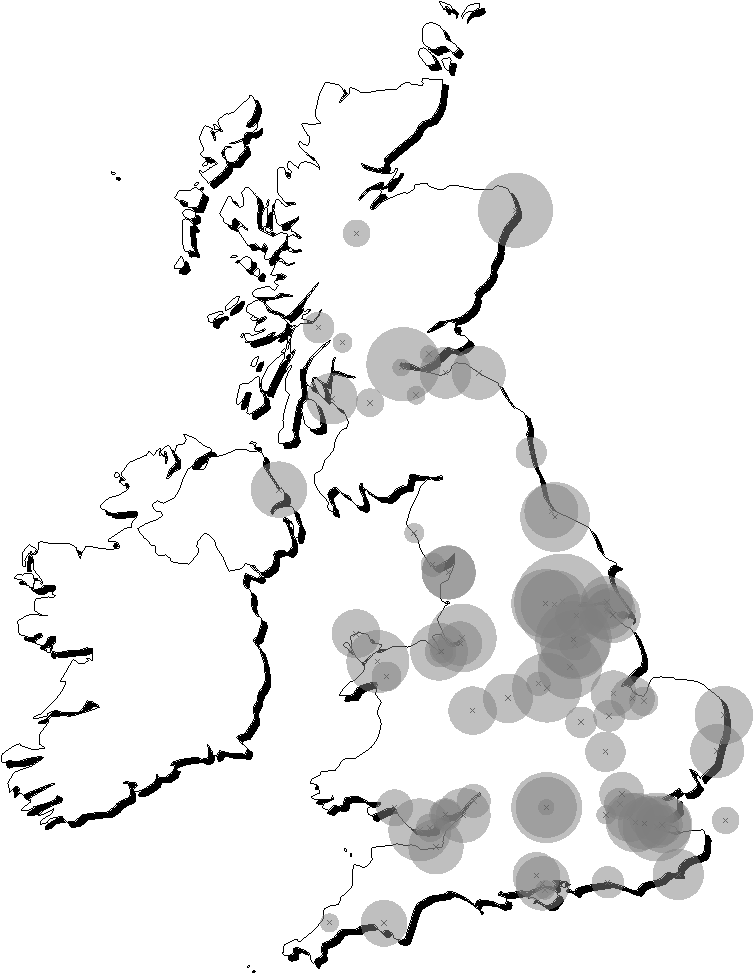
\includegraphics{figures/ngt_gen}
	  \caption{UK power station locations.}
	  \label{fig:ngt_gen}
	\end{figure}
}{}

For delivery to most consumers, electric energy is transferred at a substation
from the transmission system to the grid supply point of a distribution system.
Distribution networks in the UK are also three-phase AC power systems, but
typically operate at lower voltages and differ in their general structure (or
topology) from transmission networks.  Transmission networks are typically
highly interconnected, providing multiple paths for power flow. Distribution
networks in rural areas typically consist of long radial feeders (usually
overhead lines) and in urban areas, of many ring circuits (usually cables).
Three-phase transformers, that step the voltage down to levels more convenient
for general use (typically from 11kV or 33kV to 400V), are spaced out on the
feeders/rings. All three-phases at 400V may be provided for industrial and
commercial loads or individual phases at 230V supply typical domestic and other
commercial loads. Splitting of phases is usually planned so that each is loaded
equally. If achieved, this produces a balanced, symmetrical system with zero
current flow on the neutral and it can be analysed as a \textit{single} phase
circuit (See Section Section \ref{sec:pf_form} below).  Figure
\ref{fig:powersystem} illustrates the basic structure of a typical national
electric power system \cite{blackout04}.

\section{Electricity Markets}
The UK was the first large country to privatise its electricity supply industry
when it did so in the early 1990s.  The approach has been used as a model by
other countries and the market structures that have since been implemented in
the UK have used many of the main concepts for national electricity market
design.

The England and Wales Electricity Pool was created in 1990 to break up the
vertically integrated Central Electricity Generating Board (CEGB) and to
gradually introduce competition in generation and retail supply.
% Early adoption of electricity markets by the UK has lead to the country hosting
% many of the main European power and gas exchanges and the UK boasts a high
% degree of consumer switching compared to other European countries.
The Pool has since been
replaced by trading arrangements in which market outcomes are not centrally
determined, but arise largely from bilateral agreements between producers and
suppliers.

\subsection{The England and Wales Electricity Pool}
\label{sec:thepool}
The Electric Lighting Act 1882 initiated the development of the UK's electricity
supply industry by permitting persons, companies and local authorities to set up
supply systems, principally at the time for the purposes of street lighting and
trams.  The Central Electricity Board started operating the first grid of
interconnected regional networks (synchronised at 132kV, 50Hz) in 1933. This
began operation as a national system five years later and was nationalised in
1947.  Over 600 electricity companies were merged in the process and the British
Electricity Authority was created.  It was later dissolved and replaced with the
CEGB and the Electricity Council under The Electricity Act 1957.  The CEGB was
responsible for planning the network and generating sufficient electricity until
the beginning of privatisation.

The UK electricity supply industry was privatised, and The England and Wales
Electricity Pool created, in March 1990.  Control of the transmission system was
transferred from the CEGB to the National Grid Company, which was originally
owned by twelve regional electricity companies and has since become publicly
listed.  The Pool was a multilateral contractual arrangement between generators
and suppliers and did not itself buy or sell electricity.  Competition in
generation was introduced gradually, by first entitling customers with
consumption greater than or equal to 1MW (approximately 45\% of the non-domestic
market \cite{decc:dukes09}) to purchase electricity form any listed supplier.
This limit was lowered in April 1994 to include customers with peak loads of
100kW or more.  Finally, between September 1998 and March 1999 the market was
opened to all customers.

Scheduling of generation was on a merit order basis (cheapest first) at a day
ahead stage and set a wholesale electricity price for each half-hour period of
the schedule day.  Forecasts of total demand in MW, based on historic data and
adjusted for factors such as the weather, for each settlement period were used
by generating companies and organisations with interconnects to the England
and Wales grid to formulate bids that had to be submitted to the grid operator
by 10AM on the day before the schedule day.

\ifthenelse{\boolean{includefigures}}{\begin{figure}
\label{fig:poolbids}
\centering
\begin{tikzpicture}[thick]
  \tikzstyle{incr}=[above,sloped,text width=30mm,text centered]

  \coordinate (orig) at (0,0);
  \coordinate (y) at (0,9);
  \coordinate (x) at (10,0);

  \coordinate (p0) at (0,1);
  \coordinate (p1) at (4,1.8);
  \coordinate (p2) at (7.5,4.2);
  \coordinate (p3) at (9.5,8);

  \draw[axis] (y) node[above]{\pounds/hour} -- (orig) -- (x) node[right]{MW};

  \foreach \pnt in {p0,p1,p2,p3}
    \node[circle,draw,minimum width=4pt,inner sep=0pt,fill=black] at (\pnt) {};

%   \draw[line width=1.5pt] (p0) node[left]{$C_{noload}$} --
%   node[incr]{{\small $1^{st}$ incremental price (\pounds/MWh)}} (p1) --
%   node[incr]{{\small $2^{nd}$ incremental price (\pounds/MWh)}} (p2) --
%   node[incr]{{\small $3^{rd}$ incremental price (\pounds/MWh)}} (p3);
  \draw[line width=1.5pt] (p0) node[left]{$C_{noload}$} --
  node[incr]{$C_1$~(\pounds/MWh)} (p1) --
  node[incr]{$C_2$~(\pounds/MWh)} (p2) --
  node[incr]{$C_3$~(\pounds/MWh)} (p3);

  \draw[help lines] (p1 |- x) coordinate (cp1) -- (p1);
  \draw[help lines] (p2 |- x) coordinate (cp2) -- (p2);
  \draw[help lines] (p3 |- x) coordinate (cp3) -- (p3);

  \coordinate (c1) at (intersection of orig--x and p1--cp1);
  \coordinate (c2) at (intersection of orig--x and p2--cp2);
  \coordinate (c3) at (intersection of orig--x and p3--cp3);
  \coordinate (off) at (0,3mm);

%  \fill[red] (c1) circle (2pt);
  \draw[<->,thin] ($(orig)-(off)$) -- node[below]{$P_1$} ($(c1)-(off)$);
  \draw[<->,thin] ($(c1)-(off)$) -- node[below]{$P_2$} ($(c2)-(off)$);
  \draw[<->,thin] ($(c2)-(off)$) -- node[below]{$P_3$} ($(c3)-(off)$);

  \foreach \pnt in {orig,c1,c2,c3}
    \draw[-,thin,shorten <= 4pt] (\pnt) -- ($(\pnt)-2*(off)$);

\end{tikzpicture}
\caption{Pool bid structure.}
\end{figure}


% \begin{figure}
% \label{fig:cost_function}
% \centering
% \begin{Large}
% \begin{tikzpicture}[thick]
% %  \draw[step=1.0cm,color=gray] (0,0) grid (8,5);
% %  \node at (4.5,9.5) {Active power cost function};
%   \coordinate (y) at (0,9);
%   \coordinate (x) at (10,0);
%   \coordinate (p0) at (0,0.1);
%   \coordinate (p1) at (3.2,0.4);
%   \coordinate (p2) at (5.2,1.0);
%   \coordinate (p3) at (7,2.5);
%   \coordinate (p4) at (8.6,5);
%   \coordinate (pn) at (9.5,8.5);
%
%   \foreach \pnt in {p0,p1,p2,p3,pn}
%     \node[circle,draw,minimum width=4pt,inner sep=0pt,fill=black] at (\pnt) {};
%
% %   \draw[axis] (y) -- node[anchor=south,rotate=90,minimum size=15mm]
% %   {Cost \$/MWh} (0,0) -- node[anchor=north,minimum size=15mm] {Set-point (MW)}
% %   (x);
%   \draw[axis] (y) node[above]{$c$} -- (0,0) -- (x) node[right]{$p$};
% %  \coordinate (offprca) at ($0.8*(y)$);
% %  \coordinate (offprcb) at ($0.533*(y)$);
% %  \coordinate (offqtya) at ($.6*(x)$);
% %  \coordinate (offqtyb) at ($.9*(x)$);
% %  \draw[] let \p1=(offprca), \p2=(offqtya) in
% %  (\p1) node[left] {$\alpha$} -- (\p2);
%   \draw[line width=1.5pt] (p0) -- (p1) -- (p2) -- (p3);
%   \draw[line width=1.5pt] (p3) -- ($(p3)!0.6!(p4)$);
%   \draw[dotted] ($(p3)!0.6!(p4)$) -- ($(p3)!1.5!(p4)$);
%   \draw[dashed,line width=1.5pt,shorten >=15pt] ($(p3)!0.6!(p4)$) -- (p4);
%
%   \draw[line width=1.5pt] ($(p4)!0.4!(pn)$) -- (pn);
%   \draw[dotted] ($(p4)!-0.5!(pn)$) -- ($(p4)!0.4!(pn)$);
%   \draw[dashed,line width=1.5pt,shorten >=15pt] ($(p4)!0.4!(pn)$) -- (p4);
%
%   \draw[help lines] (p1 |- x) node[below]{$p_1$} -- (p1) -- (y |- p1)
%   node[left]{$c_1$};
%   \draw[help lines] (p2 |- x) node[below]{$p_2$} -- (p2) -- (y |- p2)
%   node[left]{$c_2$};
%   \draw[help lines] (p3 |- x) node[below]{$p_3$} -- (p3) -- (y |- p3)
%   node[left]{$c_3$};
%   \draw[help lines] (pn |- x) node[below]{$p_n$} -- (pn) -- (y |- pn)
%   node[left]{$c_n$};
%
%   \foreach \x in {2,3.5,5,6.5}
%     \draw[->,line width=2pt] (\x,6.2) -- (\x,5);
%   \node at (4.25,6.2) {$y$};
% \end{tikzpicture}
% \end{Large}
% \caption{Piecewise linear active power cost function and illustration of
% constrained cost variable minimsation, adapted from [ref].}
% \end{figure}}{}

Figure \ref{fig:poolbids} illustrates four of the five price parameters that
would make up a bid.  A start-up price would also be stated, representing the
cost of turning on the generator from cold.  The no-load price $c_{0}$
represents the cost in pounds of keeping the generator running regardless of
output. Three incremental prices $c_1$, $c_2$ and $c_3$ specify the cost in
\pounds/MWh of generation between set-points $p_1$, $p_2$ and $p_3$.

A settlement algorithm would determine an unconstrained schedule (with no
account being taken for the physical limitations of the transmission system),
meeting the forecast demand and requirements for reserve while minimising cost.
Cheapest bids up to the marginal point would be accepted first and the bid price
from the marginal generator would generally determine the system marginal price
for each settlement period.  The system marginal price would form the basis of
the prices paid by consumers and paid to generators, which would be adjusted
such that the costs of transmission are covered by the market and that the
availability of capacity is encouraged at certain times.

Variations in demand and changes in plant availability would be adjusted for by
the grid operator between day close and physical delivery, producing a
constrained schedule. Generators having submitted bids would be instructed to
increase or reduce production as appropriate.  Alternatively, the grid operator
could instruct large customers with contracts to curtail their demand to do so
or instruct generators contracted to provide ancillary services to adjust
production.

\subsection{British Electricity Transmission and Trading Arrangements}
% \subsection{New Electricity Trading Arragements}
\label{sec:betta}
Concerns over the exploitation of market power in The England and Wales
Electricity Pool and over the ability of the market to reduce consumer
electricity prices prompted the introduction of New Electricity Trading
Arrangements (NETA) in March 2001 \cite{martoccia:2005}.  The aim was to improve
efficiency and provide greater choice to participants.  Control of the Scottish
transmission system was included with the introduction of the nationwide British
Electricity Transmission and Trading Arrangements (BETTA) in April 2005 under
The Energy Act 2004.  While The Pool operated a single daily auction and
dispatched plant centrally, under the new arrangements participants became
self-dispatching and market positions became determined through continuous
bilateral trading between generators, suppliers, traders and consumers.

The majority of power is traded under the BETTA through long-term contracts that
are customised to the requirements of each party \cite{kirschen:book}. These
instruments suit participants responsible for large power stations or those
purchasing large volumes of power for many customers.  Relatively, large
amounts of time and effort are typically required for these long-term contracts to be initially
formed and this results in a high associated transaction cost. However, they
reduce risk for large players and often include a degree of flexibility.

Electric power is also traded directly between participants through
over-the-counter contracts that usually have a standardised form.  Such
contracts typically concern smaller volumes of power and have lower
associated transaction costs.  Often they are used by participants to refine
their market position ahead of delivery time \cite{kirschen:book}.

Trading facilities, such as power exchanges, provide a means for participants
to fine-tune their positions further, through short-term transactions for
often relatively small quantities of energy.  Modern exchanges are
computerised and accept anonymous offers and bids submitted electronically.
% A submitted offer/bid will be paired with any outstanding bids/offers in the
% system with compatible price and quantity values.  The details are then
% displayed for traders to observe and to use in subsequent trading.

All bilateral trading must be completed before ``gate-closure'': a point in time
before delivery that gives the system operator an opportunity to balance supply
and demand and mitigate potential breaches of system limits.  In keeping with
the UK's free market philosophy, a competitive spot market \cite{schweppe:spot}
forms part of the balancing mechanism.  A generator that is not fully loaded
may offer a price at which it is willing to increase its output by a specified
quantity, stating the rate at which it is capable of doing so.  Certain loads
may also offer demand reductions at a price which can typically be implemented
very quickly.  Longer-term contracts for balancing services are also struck
between the system operator and generators/suppliers in order to avoid the price
volatility often associated with spot markets.

\section{Electricity Market Simulation}
Previous sections have identified the importance of electricity to modern
societies and explained how the majority of electricity supply in the UK is
trusted to unadministered bilateral trade.  All aspects of electricity supply
are constantly changing and electricity markets must be suitably researched to
ensure that their designs are fit for purpose.  The value of electricity to
society means that it is not practical to experiment with radical changes to
trading arrangements on real systems.
% A practical alternative is to study abstract mathematical models (with sets of
% simplifying approximations and assumptions) and find analytical solutions,
% where possible, by simulating them using computer programs.

Game theory is the branch of applied mathematics in which behaviour in strategic
situations is captured mathematically.  A common approach to doing this is to
model the system and players as a mathematical optimisation problem.  Optimal
power flow is a classic optimisation problem in the field of Electrical Power
Engineering and variants of it are widely used in electricity market research.
In this thesis, optimal power flow forms part of an \textit{agent-based}
simulation: an alternative approach to the mathematics of games.

\subsection{Agent-Based Simulation}
Social systems, such as electricity markets, are inherently complex and involve
interactions between different types of individual and between individuals and
collective entities, such as organisations or groups, the behaviour of which is
itself the product of individual interactions.  This complexity drives classical
monolithic equilibrium models to their limits.  The models are often highly
stylised and limited to small numbers of players with strong constraining
assumptions made on their behaviour.

Agent-based simulation involves modelling the simultaneous operations of, and
interactions between adaptive agents and then assessing their effect on the
system as a whole.  System properties arise from agent interactions, even those
with simple behavioural rules, that could not be deduced by simply aggregating
the agent's properties. % Game of Life

Following \citeA{tesfatsi:handbook}, the objectives of agent-based modelling
research fall roughly into four strands: empirical, normative, heuristic and
methodological. The \textit{empirical} objectives are to understand how and why
macro-level regularities have evolved from micro-level interactions when little
or no top-down control is present.  Research with \textit{normative} goals aims
to relate agent-based models to an ideal standard or optimal design.  The
objective being to evaluate proposed designs for social policy, institutions or
processes in their ability to produce socially desirable system performance. The
\textit{heuristic} strand aims to generate theories on the fundamental causal
mechanisms in social systems that can be observed when there are alternative
initial conditions.  This thesis aims to provide \textit{methodological}
advancement.  Improvements in the tools and methods available aids research with
the former objectives.

\subsection{Optimal Power Flow}
\label{sec:opf}
Nationalised electricity supply industries were for many years planned, operated
and controlled centrally.  A system operator would determine which generators
must operate and the required output of the operating units such that demand and
reserve requirements were met and the overall cost of production was minimised.
In Electric Power Engineering, these are termed the \textit{unit commitment} and
\textit{economic dispatch} problems.

A formulation of the unit commitment problem was published in 1962 that
incorporated electric power system constraints \cite{carpentier:opf}.  Optimal
power flow is this combination of the economic and power flow aspects of power
systems into one mathematical optimisation problem.  The ability of optimal
power flow to solve centralised power system operation problems and determine
prices in power pool markets has resulted in it becoming one of the most widely
studied subjects in the electric power systems community.

\subsubsection{Power Flow Formulation}
\label{sec:pf_form}
Optimal power flow derives its name from the power flow (or load flow)
steady-state power system analysis technique.  Given sets of generator data,
load data and a nodal admittance matrix, a power flow study determines the
complex voltage
\begin{equation}
V_i = \vert V_i \vert \angle\delta_i = \vert
V_i\vert(\cos\delta_i + j\sin\delta_i)
\end{equation}
at each node $i$ in the power system, from which line flows may be calculated
\cite{grainger:psa}.

\paragraph{Nodal Admittance Matrix}
The nodal admittance matrix describes the electrical network and its formulation
is dependant upon the transmission line, transformer and shunt models employed.
A branch in a nodal representation of a power system is typically modelled as a
medium length transmission line in series with a regulating transformer at the
``from'' end \cite[p.11]{pserc:mp_manual}. A nominal-$\pi$ model with total
series admittance $y_s = 1/(r_s+jx_s)$ and total shunt capacitance $b_c$ is
often to represent the transmission line.  The transformer may assumed to be
ideal, phase-shifting and tap-changing, with the ratio between primary winding
voltage $v_{f}$ and secondary winding voltage $N = \tau e^{j\theta_{ph}}$ where
$\tau$ is the tap ratio and $\theta_{ph}$ is the phase shift angle. Figure
\ref{fig:branch_model} diagrams this conventional branch model.  From
Kirchhoff's Current Law the current in the series impedance is
\begin{equation}
\label{eq:iseries}
i_s = \frac{b_c}{2}v_t - i_t
\end{equation}
and from Kirchhoff's Voltage Law the voltage across the secondary winding of
the transformer is
\begin{equation}
\frac{v_{f}}{N} = v_t + \frac{i_s}{y_s}
\end{equation}
Substituting $i_s$ from equation (\ref{eq:iseries}), gives
\begin{equation}
\label{eq:vfrom}
\frac{v_{f}}{N} = v_t - \frac{i_t}{y_s} + v_t\frac{b_c}{2y_s}
\end{equation}
and rearranging in terms if $i_t$, gives
\begin{equation}
\label{eq:ito}
i_t = v_s \left( \frac{-y_s}{\tau e^{\theta_{ph}}} \right) +
v_r \left( y_s + \frac{b_c}{2} \right)
\end{equation}
The current through the secondary winding of the transformer is
\begin{equation}
N^*i_f = i_s + \frac{b_c}{2}\frac{v_{f}}{N}
\end{equation}
Substituting $i_s$ from equation (\ref{eq:iseries}) again, gives
\begin{equation}
N^*i_f = \frac{b_c}{2}v_t - i_t + \frac{b_c}{2}\frac{v_{f}}{N}
\end{equation}
and substituting $\frac{v_{f}}{N}$ from equation (\ref{eq:vfrom}) and
rearranging in terms if $i_s$, gives
\begin{equation}
\label{eq:ifrom}
i_s = v_s \left( \frac{1}{\tau^2} \left(y_s + \frac{b_c}{2}\right) \right) +
v_r \left(\frac{y_s}{\tau e^{-j\theta}}\right)
\end{equation}

\ifthenelse{\boolean{includefigures}}{\begin{figure}
\centering
\begin{tikzpicture}[thick]
%   \def\capacitor(#1,#2){%
%     \draw (#1,#2+3cm) -- (#1,#2+5mm);
% %    \draw (#1-1cm,#2+5mm) -- (#1+1cm,#2+5mm);
% %     \draw[linewidth=1pt] (-1cm,-5mm) -- (1cm,-5mm);
% %     \draw[linewidth=1pt] (0,-1cm) -- (0,-5mm);
%   }
%
%   \capacitor(0,0);

%   \def\terminal(#1,#2){#3}{%
%     \node[circle,draw,minimum width=5pt,inner sep=0pt] (#3) at (#1,#2) {};
%   }
%   \terminal(5,5);

  \coordinate (vf0) at (0,0);
  \coordinate (vf+) at (0,6);
  \coordinate (vt0) at (13,0);
  \coordinate (vt+) at (13,6);

  \coordinate (trx) at (2,3);
  \coordinate (vf0p) at ($(trx)-(0.5,3)$);
  \coordinate (vf+p) at ($(trx)+(-0.5,3)$);
  \coordinate (vf0s) at ($(trx)-(-0.5,3)$);
  \coordinate (vf+s) at ($(trx)+(0.5,3)$);

  \coordinate (vl0) at (4,0);
  \coordinate (vl+) at (4,6);
  % resistor
  \coordinate (res) at (7.5,6);
  \coordinate (rin) at ($(res) -(7mm,0)$);
  \coordinate (rout) at ($(res) + (7mm,0)$);
  \coordinate (rh) at (0,6pt);
  % inductor
  \coordinate (ind) at (9.5,6);
  \coordinate (lin) at ($(ind)-(7mm,0)$);
  \coordinate (lout) at ($(ind)+(7mm,0)$);

  \coordinate (capw) at (7mm,0);
  \coordinate (bc1) at (5.8,3);
  \coordinate (bc1in) at ($(bc1) + (0,2mm)$);
  \coordinate (bc1out) at ($(bc1) - (0,2mm)$);
  \coordinate (bc2) at (11.2,3);
  \coordinate (bc2in) at ($(bc2) + (0,2mm)$);
  \coordinate (bc2out) at ($(bc2) - (0,2mm)$);

  \node[circle,draw,minimum width=4pt,inner sep=0pt] (nvf0) at (vf0) {};
  \node[circle,draw,minimum width=4pt,inner sep=0pt] (nvf+) at (vf+) {};
  \node[circle,draw,minimum width=4pt,inner sep=0pt] (nvl0) at (vl0) {};
  \node[circle,draw,minimum width=4pt,inner sep=0pt] (nvl+) at (vl+) {};
  \node[circle,draw,minimum width=4pt,inner sep=0pt] (nvt0) at (vt0) {};
  \node[circle,draw,minimum width=4pt,inner sep=0pt] (nvt+) at (vt+) {};

  \draw (nvl0) -- (nvt0);
  % transformer
  \draw (nvf0) -- (vf0p);
  \draw (vf0s) -- (nvl0);
  \draw (nvf+) -- (vf+p);
  \draw (vf+s) -- (nvl+);
  \draw[decorate,decoration={coil,amplitude=5pt,segment length=5.5pt,
  pre length=10mm,post length=10mm}] (vf+p) -- (vf0p);
  \draw[decorate,decoration={coil,amplitude=5pt,segment length=5.5pt,
  pre length=10mm,post length=10mm}] (vf0s) -- (vf+s);
  \coordinate (cor1) at ($(trx)-(1mm,0)$);
  \coordinate (cor2) at ($(trx)+(1mm,0)$);
  \coordinate (corh) at (0,1.8);
  \draw[line width=1.5pt] ($(cor1)-(corh)$) -- ($(cor1)+(corh)$);
  \draw[line width=1.5pt] ($(cor2)-(corh)$) -- ($(cor2)+(corh)$);

  % resistor
  \filldraw[fill=white,drop shadow] ($(rin)-(rh)$) rectangle ($(rout)+(rh)$);
  \draw ($(res) + (0,5mm)$) node {$r_s$};
  \draw (nvl+) -- (rin);

  \draw (rout) -- (lin);
  % inductor
  \draw[decorate,decoration={coil,amplitude=6pt,segment length=6pt}]
  (lin) -- (lout);
  \draw ($(ind) +(0,5mm)$) node {$x_s$};
  \draw (lout) -- (nvt+);
  % capacitor 1
  \draw (bc1in) -- (bc1in |- vf+s) node[circle,draw,minimum width=2pt,
  inner sep=0pt,fill=black]{};
  \draw (bc1out) -- (bc1out |- vf0s) node[circle,draw,minimum width=2pt,
  inner sep=0pt,fill=black]{};
  \draw[line width=1.2pt] ($(bc1in)-(capw)$) -- ($(bc1in)+(capw)$);
  \draw[line width=1.2pt] ($(bc1out)-(capw)$) -- ($(bc1out)+(capw)$);
%   \draw[line width=1.2pt] ($(bc1out)$) .. controls ($(bc1out)+(capw)+(-2mm,0)$)
%   .. ($(bc1out)+(capw)+(0,-2mm)$); \draw ($(bc1) + (capw)$) node[anchor=west] {$\dfrac{b_c}{2}$};
  % capacitor 2
  \draw (bc2in) -- (bc2in |- vt+) node[circle,draw,minimum width=2pt,
  inner sep=0pt,fill=black]{};
  \draw (bc2out) -- (bc2out |- vt0) node[circle,draw,minimum width=2pt,
  inner sep=0pt,fill=black]{};
  \draw[line width=1.2pt] ($(bc2in)-(capw)$) -- ($(bc2in)+(capw)$);
  \draw[line width=1.2pt] ($(bc2out)-(capw)$) -- ($(bc2out)+(capw)$);
  \draw ($(bc2) - (capw)$) node[anchor=east] {$\dfrac{b_c}{2}$};

  \draw[->,shorten >=5pt,shorten <=5pt,thin] (vf0) node[above right] {$-$} --
  node[fill=white] {$v_f$} (vf+) node[below right] {$+$};
  \draw[->,shorten >=5pt,shorten <=5pt,thin] (vl0) node[above left] {$-$} --
  node[fill=white] {$\dfrac{v_f}{N}$} (vl+) node[below left] {$+$};
  \draw[->,shorten >=5pt,shorten <=5pt,thin] (vt0) node[above left] {$-$} --
  node[fill=white] {$v_t$} (vt+) node[below left] {$+$};
  \node at ($(trx)-(0,2.4)$) {$N:1$};
  \draw[->,thin] ($(vf+)+(rh)$) -- node[above]{$i_f$} ++(12mm,0);
  \draw[->,thin] ($(vf+s)+(rh)$) -- node[above]{$N^*i_f$} ++(12mm,0);
  \draw[->,thin] ($(vt+)+(rh)$) -- node[above]{$i_t$} ++(-12mm,0);
  \draw[->,thin] ($(lout)+(rh)$) -- node[above]{$i_l$} ++(8mm,0);

\end{tikzpicture}
\caption{Nominal-$\pi$ transmission line model in series with a phase
shifting transformer model.}
\label{fig:branch_model}
\end{figure}}{}

Combining equations (\ref{eq:ito}) and (\ref{eq:ifrom}), the \textit{from} and
\textit{to} end complex current injections for branch $l$ are
\begin{equation}
\label{eq:ybranch}
\begin{bmatrix}
i_f^l\\
i_t^l
\end{bmatrix}
=
\begin{bmatrix}
y_{ff}^l& y_{ft}^l\\
y_{tf}^l& y_{tt}^l
\end{bmatrix}
\begin{bmatrix}
v_f^l\\
v_t^l
\end{bmatrix}
\end{equation}
where
\begin{eqnarray}
\label{eq:yff}
y_{ff}^l& =& \frac{1}{\tau^2} \left(y_s + \frac{b_c}{2}\right)\\
\label{eq:yft}
y_{ft}^l& =& \frac{y_s}{\tau e^{-j\theta_{ph}}}\\
\label{eq:ytf}
y_{tf}^l& =& \frac{-y_s}{\tau e^{j\theta_{ph}}}\\
\label{eq:ytt}
y_{tt}^l& =& y_s + \frac{b_c}{2}
\end{eqnarray}
Let $Y_{ff}$, $Y_{ft}$, $Y_{tf}$ and $Y_{tt}$ be $n_l \times 1$ vectors where
the $l^{th}$ element of each corresponds to $y_{ff}^l$, $y_{ft}^l$,
$y_{tf}^l$ and $y_{tt}^l$, respectively.  Furthermore, let $C_f$ and $C_t$ be the
$n_l \times n_b$ branch-bus connection matrices, where $C_{fij} = 1$ and
$C_{tik} = 1$ if branch $i$ connects from bus $j$ to bus $k$
\cite[p.12]{pserc:mp_manual}.  The $n_l \times n_b$ branch admittance matrices
are
\begin{eqnarray}
Y_f& =& \diag(Y_{ff})C_f + \diag(Y_{ft})C_t\\
Y_t& =& \diag(Y_{tf})C_f + \diag(Y_{tt})C_t
\end{eqnarray}
and the
$n_b \times n_b$ nodal admittance matrix is
\begin{eqnarray}
Y_{bus}& =& C_f^\mathsf{T} Y_f + C_t^\mathsf{T} Y_t .
\end{eqnarray}
% and it relates the complex bus voltages to the nodal current injections
% \begin{eqnarray}
% I_{bus}& =& Y_{bus}V
% \end{eqnarray}
% The complex bus power injections are expressed as a non-linear function of $V$
% \begin{eqnarray}
% S_{bus}(V)& =& \diag(V)I_{bus}^* \nonumber \\
% \label{eq:sbus}
% &= & \diag(V)Y_{bus}^*V^*
% \end{eqnarray}
% The net complex power injection (generation - load) at each bus must equal the
% sum of complex power flows on each branch connected to the bus.  Hence the AC
% power balance equations are
% \begin{equation}
% \label{eq:mismatch}
% S_{bus}(V) + S_d - S_g = 0
% \end{equation}

\paragraph{Power Balance}
% Importantly, the relationship between nodal voltages and power entering the
% network is non-linear.
For a network of $n_b$ nodes, the current injected at
node $i$ is
\begin{equation}
I_i = \sum_{j=1}^{n_b} Y_{ij} V_j
\end{equation}
where $Y_{ij} = \vert Y_{ij}\vert \angle\theta_{ij}$ is the $(i,j)^{th}$ element
if the $Y_{bus}$ matrix.  Hence, the apparent power entering
the network at bus $i$ is
\begin{equation}
S_i = P_i+Q_i = V_iI_i^* = \sum_{n=1}^{n_b} \vert Y_{ij}V_iV_j \vert \angle
(\delta_i - \delta_j - \theta_{ij})
\end{equation}
Converting to polar coordinates and separating the real and imaginary parts,
the active power
\begin{equation}
P_i = \sum_{n=1}^{n_b} \vert Y_{ij}V_iV_j \vert \cos(\delta_i - \delta_j -
\theta_{ij})
\end{equation}
and the reactive power
\begin{equation}
Q_i = \sum_{n=1}^{n_b} \vert Y_{ij}V_iV_j \vert \sin(\delta_i - \delta_j -
\theta_{ij})
\end{equation}
entering the network at bus $i$ are non-linear functions of $V_i$, as indicated
by the presence of the sine and cosine terms.  Kirchhoff's Current Law requires
that the net complex power injection (generation - load) at each bus equals the sum of
complex power flows on each branch connected to the bus.  The power balance
equations
\begin{equation}
\label{eq:p_balance}
P_g^i - P_d^i = P^i
\end{equation}
and
\begin{equation}
\label{eq:q_balance}
Q_g^i - Q_d^i = Q^i,
\end{equation}
where the subscripts $g$ and $d$ indicate generation and demand
respectively, form the principal non-linear constraints in the optimal power
flow problem.

% \paragraph{DC Power Flow}
% The power balance equations may be linearised and problem of solving them
% greatly simplified if the following additional assumptions are made
% \cite[p.14]{pserc:mp_manual}:
% \begin{itemize}
%   \item The resistance $r_s$ and shunt capacitance $b_c$ of all branches can be
%   considered negligible.
%   \begin{equation}
%   \label{eq:lossless}
%   y_s \approx \frac{1}{jx_s}, \quad b_c \approx 0
%   \end{equation}
%   \item Bus voltage magnitudes $v_{m,i}$ are all approximately 1 per-unit.
%   \begin{equation}
%   \label{eq:oneperunit}
%   v_i \approx 1e^{j\theta_i}
%   \end{equation}
%   \item The voltage angle difference between bus $i$ and bus $j$ is small enough
%   that
%   \begin{equation}
%   \label{eq:busangdiff}
%   \sin\theta_{ij} \approx \theta_{ij}
%   \end{equation}
% \end{itemize}
% Applying the assumption that branches are lossless from equation
% (\ref{eq:lossless}), the quadrants of the branch admittance matrix in equations
% (\ref{eq:yff}), (\ref{eq:yft}), (\ref{eq:ytf}) and (\ref{eq:ytt}), approximate
% to
% \begin{eqnarray}
% y_{ff}^l& =& \frac{1}{jx_s \tau^2}\\
% y_{ft}^l& =& \frac{-1}{jx_s \tau e^{-j\theta_{ph}}}\\
% y_{tf}^l& =& \frac{-1}{jx_s \tau e^{j\theta_{ph}}}\\
% y_{tt}^l& =& \frac{1}{jx_s}
% \end{eqnarray}
% respectively.  Applying the uniform bus voltage magnitude assumption from
% equation (\ref{eq:oneperunit}) to equation (\ref{eq:ybranch}), the branch
% ``from'' end current approximates to
% \begin{eqnarray}
% i_f& \approx& \frac{e^{j\theta_f}}{jx_s\tau^2} -
% \frac{e^{j\theta_t}}{jx_s \tau e^{-j\theta_{ph}}}\\
% & =& \frac{1}{jx_s\tau} ( \frac{1}{\tau}e^{j\theta_f} -
% e^{j(\theta_t + \theta_{ph})} )
% \end{eqnarray}
% % ToDo: Branch to end current derivation.
% and the branch ``from'' end complex power flow $s_f = v_f \cdot i_f^*$
% approximates to
% \begin{eqnarray}
% s_f& \approx& e^{j\theta_f} \cdot \frac{j}{x_s\tau}
% (\frac{1}{\tau}e^{-j\theta_f} - e^{j(\theta_t + \theta_{ph})})\\
% & =& \frac{1}{x_s\tau} \left[ \sin(\theta_f-\theta_t-\theta_{ph}) +
% j\left( \frac{1}{\tau} - \cos(\theta_f-\theta_t-\theta_{ph}) \right) \right]
% \end{eqnarray}
% Applying the voltage angle difference assumption from equation
% (\ref{eq:busangdiff}) yields the approximation
% \begin{equation}
% p_f \approx \frac{1}{x_s\tau}(\theta_f-\theta_t-\theta_{ph})
% \end{equation}
% Let $B_{ff}$ and $P_{f,ph}$ be the $n_l \times 1$ vectors where
% $B_{ff_i} = 1 / (x_s^i\tau^i)$ and $P_{f,ph_i} =
% -\theta_{ph}^i / (x_s^i\tau^i)$.  Then if the system $B$ matrices are
% \begin{eqnarray}
% B_f& =& \diag(B_{ff})(C_f-C_t)\\
% B_{bus}& = &(C_f-C_t)^\mathsf{T}B_f
% \end{eqnarray}
% then the real power bus injections are
% \begin{equation}
% \label{eq:bbus}
% P_{bus}(\Theta) = B_{bus}\Theta + P_{bus,ph}
% \end{equation}
% where $\Theta$ is the $n_b \times 1$ vector of bus voltage angles and
% \begin{equation}
% P_{bus,ph} = (C_f-C_t)^\mathsf{T} + P_{f,ph}
% \end{equation}
% The active power flows at the branch ``from'' ends are
% \begin{equation}
% \label{eq:pf_loss}
% P_f(\Theta) = B_f\Theta + P_{f,ph}
% \end{equation}
% and $P_t = -P_f$ since all branches are assumed lossless.

\subsubsection{Optimal Power Flow Formulation}
Optimal power flow is a mathematical optimisation problem constrained by the
complex power balance equations (\ref{eq:p_balance}) and (\ref{eq:q_balance}).
Mathematical optimisation problems have the general form
\begin{equation}
\min_x f(x)
\end{equation}
subject to
\begin{eqnarray}
\label{eq:equality}
g(x)& =& 0\\
\label{eq:inequality}
h(x)& \leq& 0
\end{eqnarray}
where $x$ is the vector of optimisation variables, $f$ is the objective
function and equations (\ref{eq:equality}) and (\ref{eq:inequality}) are sets
of equality and inequality constraints, respectively, on $x$.

In optimal power flow, typical inequality
constraints are bus voltage magnitude contingency state limits, generator
output limits and branch power or current flow limits.  The vector of
optimisation variables $x$ may consist of generator set-points, bus voltages,
transformer tap settings etc.  If $x$ is empty then
the formulation reduces to the general power flow problem described above.

% Branch complex power flow limits $S_{max}$ are enforced by the inequality
% constraints
% \begin{eqnarray}
% \abs{S_f(V)} - S_{max}& \leq &0\\
% \abs{S_f(V)} - S_{max}& \leq &0
% \end{eqnarray}
% and the reference bus voltage angle $\theta_i$ is fixed with the equality
% constraint
% \begin{equation}
% \label{eq:refbusang}
% \theta_i^{ref} \leq \theta_i \leq \theta_i^{ref}, \quad i \in \mathcal{I}_{ref}
% \end{equation}
% Upper and lower limits on the optimisation variables $V_m$, $P_g$ and $Q_g$ are
% enforced by the inequality constraints
% \begin{eqnarray}
% v_m^{i,min} \leq v_m^i \leq v_m^{i,max},& \quad i= 1 \dotsc n_b&\\
% \label{eq:pglim}
% p_g^{i,min} \leq p_g^i \leq p_q^{i,max},& \quad i= 1 \dotsc n_g&\\
% q_g^{i,min} \leq q_g^i \leq q_q^{i,max},& \quad i= 1 \dotsc n_g&
% \end{eqnarray}

A common objective in the optimal power flow problem is total system cost
minimisation. For a network of $n_g$ generators the objective function is
\begin{equation}
\label{eq:objfunc}
\min_{\theta, V_m, P_g, Q_g} \sum_{k=1}^{n_g} c^k_P(p_g^k) + c_Q^k(q_g^k)
\end{equation}
where $c_P^k$ and $c_Q^k$ are cost functions (typically quadratic) of the
set-points $p_g^k$ and $q_g^k$ for generator $k$, respectively. Alternative
objectives may be to minimise losses, maximise the voltage stability margin or
minimise deviation of an optimisation variable from a particular schedule
\cite[\S18]{kallrath:2009}.

\subsubsection{Nodal Marginal Prices}
Many solution methods for optimal power flow have been developed since the
problem was introduced by \citeA{carpentier:opf} and a review of the main
techniques can be found in \citeA{momoh:part1,momoh:part2}. One of the most
robust strategies is to solve the Lagrangian function
\begin{equation}
\mathcal{L}(x) = f(x) + \lambda^\mathsf{T}g(x) + \mu^\mathsf{T}h(x),
\end{equation}
where $\lambda$ and $\mu$ are vectors of Lagrangian multipliers, using an
Interior Point Method \cite{cvxopt:2004}.  When solved, the Lagrangian
multiplier for a constraint gives the rate of change of the objective function value with respect to the
constraint variable.  If the objective function is equation (\ref{eq:objfunc}), the Lagrangian
multipliers $\lambda^i_P$ and $\lambda^i_Q$ for the power balance constraint at
each bus $i$, given by equations (\ref{eq:p_balance}) and (\ref{eq:q_balance}),
are the nodal marginal prices and can be interpreted as the increase in the
total system cost for and additional injection at $i$ of 1MW or 1MVAr,
respectively.

For a case in which none of the inequality constraints $h(x)$
(such as branch power flow or bus voltage limits) are binding, the nodal
marginal prices are uniform across all buses and equal the cost of the
marginal generating unit.  When the constraints \textit{are} binding, the nodal
marginal prices are elevated for buses at which adjustments to power injection
are required for the constraints to be satisfied.  Nodal marginal prices are
commonly used in agent-based electricity market simulation to determine the
revenue for generating units as they reflect the increased value of production in
constrained areas of the power system.

\newpage
\section{Reinforcement Learning}
\label{sec:rl}
% The problem of learning how best to interact with an environment so as to
% maximise some long-term reward is a general one.  Reinforcement learning is a
% term from the field of machine learning that is typically applied to
% understanding, automating and solving this problem through adaptive
% computational approaches.  Unlike many machine learning techinques, the
% algorithms are not instructed as to which actions to take, but must learn to
% maximise the long-term reward through trial-and-error.

% Reinforcement learning starts with an interactive, goal-seeking individual
% agent existing in an environment.  The agent requires the ability to;
% \begin{itemize} \item Sense aspects of its environment, \item Perform actions
% that influence the state of its environment and \item be assigned rewards as a
% response to their chosen action. \end{itemize} An agent follows a particular
% \textit{policy} when mapping the perceived state of its environment to an
% action choice.  Reinforcement learning methods adjust the agent's policy.
Reinforcement learning is learning from reward by mapping situations to actions
when interacting with an uncertain environment \cite{suttonbarto:1998}.  An
agent learns \textit{what} to do in order to achieve a task through
trial-and-error using a numerical reward or a penalty signal without being
instructed \textit{how} to achieve it.  Some actions may not yield immediate
reward or may effect the next situation and all subsequent rewards.  Always, a
compromise must be made between the exploitation of past experiences and the
exploration of the environment through new action choices. In reinforcement
learning an agent must be able to:
\begin{itemize}
  \item Sense aspects of its environment,
  \item Take actions that influence its environment and,
  \item Have an explicit goal or set of goals relating to the state of its
  environment.
\end{itemize}

In the classical model of agent-environment interaction, at each time step $t$
in a sequence of discrete time steps $t = 1,2,3\dotsc$ an agent receives as
input some form of the environment's state $s_t \in \mathscr{S}$, where
$\mathscr{S}$ is the set of possible states.  From a set of actions
$\mathscr{A}(s_t)$ available to the agent in state $s_t$ and the agent selects
an action $a_t$ and performs it in its environment.  The environment enters a
new state $s_{t+1}$ in the next time step and the agent receives a scalar
numerical reward $r_{t+1} \in \mathbb{R}$ in part as a result of its action.
The agent then learns from the state representation, the
chosen action $a_t$ and the reinforcement signal $r_{t+1}$ before beginning
its next interaction.  Figure \ref{fig:seq_rl} diagrams the classical
agent-environment interaction event sequence in reinforcement learning.

\ifthenelse{\boolean{includefigures}}{\begin{figure}
  \centering
  \begin{sequencediagram}
    \newthread{agt}{:Agent}
    \newinst[3]{env}{:Environment}
    \begin{sdblock}{Interaction}{}

      \begin{call}{agt}{getState()}{env}{$s_t$}
      \end{call}

      \begin{callself}{agt}{chooseAction($s_t$)}{$a_t$}
      \end{callself}

      \begin{call}{agt}{performAction($a_t$)}{env}{$r_{t+1}$}
        \begin{callself}{env}{changeState($a_t$)}{$s_{t+1}$}
        \end{callself}
      \end{call}

      \begin{callself}{agt}{learn($s_t$,$a_t$,$r_{t+1}$)}{}
      \end{callself}

    \end{sdblock}
  \end{sequencediagram}
  \caption{Sequence diagram for the basic reinforcement learning model.}
  \label{fig:seq_rl}
\end{figure}
}{}

% \subsection{Markov Decision Processes}
For a finite number of states, if all states are Markov, the agent interacts
with a finite Markov decision process (MDP).  Informally, for a state to be
Markov it must retain all relevant information about the complete sequence of
positions leading up to the state, such that all future states and expected
rewards can be predicted as well as would be possible given a complete history
\cite{suttonbarto:1998}.  A particular MDP is defined for a discrete set of time
steps by a state set $\mathscr{S}$, an action set $\mathscr{A}$, a set of state
transition probabilities $\mathscr{P}$ and a set of expected reward values
$\mathscr{R}$.
% Given a state $s$ and an action $a$, the probability of transitioning to each
% possible next state $s^\prime$ is \begin{equation} \mathscr{P}^a_{ss^\prime} =
% \Pr \bigl\lbrace s_{t+1} = s^\prime \vert s_t=s, a_t=a \bigr\rbrace .
% \end{equation} Given the next state $s^\prime$, the expected value of the next
% reward is \begin{equation} \mathscr{R}^a_{ss^\prime} = E \bigl\lbrace r_{t+1}
% \vert s_t=s, a_t=a, s_{t+1}=s^\prime \bigr\rbrace . \end{equation}
In practice not all state signals are Markov, but should provide a good basis
for predicting subsequent states, future rewards and selecting actions.

If the state transition probabilities and expected reward values are not known,
only the states and actions, then samples from the MDP must be taken and a value
function approximated iteratively based on new experiences generated by
performing actions.

\subsection{Value Function Methods}
\label{sec:valuebased}
% Value-based methods attempt to find the optimal policy by
% approximating a \textit{value-function} which returns the total reward an
% agent can expect to accumulate, given an initial state and following the
% current policy thereafter.  The policy is adjusted using the reinforcing
% signal and information from previous action choices.
Any method that can optimise control of a MDP may be considered a reinforcement
learning method.  All search for an optimal policy $\pi^*$ that maps state
$s \in \mathscr{S}$ and action $a \in \mathscr{A}$ to the probability
$\pi^*(s,a)$ of taking $a$ in $s$ and maximises the sum of rewards over the
agents lifetime.

Each state $s$ under policy $\pi$ may be associated with a \textit{value}
$V^\pi(s)$ equal to the expected return from following policy $\pi$ from state
$s$.  Most reinforcement learning methods are based on estimating the
state-value function
\begin{equation}
\label{eq:statevalue}
V^\pi(s) = E \Bigg\lbrace \sum^\infty_{t=0} \gamma^t r_t \Bigg\vert s_0 = s
\Bigg\rbrace
\end{equation}
where $\gamma$ is a discount factor, with $0\leq \gamma \leq 1$ and $E$
indicates that it is an estimate. Performing certain actions may result in no
state change, creating a loop and causing the value of that action to be infinite for certain policies.
The discount factor $\gamma$ prevents values from going unbounded and
represents reduced trust in the reward $r_t$ as discrete time $t$
increases.  Many reinforcement learning methods estimate the action-value
function
\begin{equation}
\label{eq:actionvalue}
Q^\pi(s,a) = E \Bigg\lbrace \sum^\infty_{t=0} \gamma^t r_t \Bigg\vert s_0 = s,
a_0 = a \Bigg\rbrace
\end{equation}
which defines the value of taking action $a$ in state $s$ under fixed policy
$\pi$.

\subsubsection{Temporal-Difference Learning}
Temporal Difference (TD) learning is a fundamental concept in reinforcement
learning that was introduced by \citeA{suttonbarto:1998}. TD methods do not
attempt to estimate the state transition probabilities and expected rewards of
the finite MDP, but estimate the value function directly. They learn to
\textit{predict} the expected value of total reward returned by the state-value
function (\ref{eq:statevalue}).  For an exploratory policy $\pi$ and a
non-terminal state $s$, an estimate of $V^\pi(s_t)$ at any given time step $t$
is updated using the estimate at the next time step $V^\pi(s_{t+1})$ and the
observed reward $r_{t+1}$
\begin{equation}
V^\pi(s_t) = V^\pi(s_t) + \alpha \bigl[r_{t+1} + \gamma
V^\pi(s_{t+1}) - V^\pi(s_t) \bigr]
\end{equation}
where $\alpha$ is the learning rate, with $0 \leq \alpha \leq 1$, which controls
how much attention is paid to new data when updating $V^\pi$.  Plain TD
learning evaluates a particular policy and offers strong convergence
guarantees, but does not learn better policies.

\subsubsection{Q-Learning}
\label{sec:qlearning}
% This section describes the original off-policy Temporal Difference Q-learning
% method developed by Watkins \cite{watkins:1989}.  The action-value function,
% $Q(s,a)$, returns values from a $M \times N$ matrix where $M$ and $N$ are
% arbitrary positive numbers equal to the total number of feasible states and
% actions, respectively.  Each value represents the \textit{quality} of taking a
% particular action, $a$, in state $s$.  Actions are selected using either the
% $\epsilon$-greedy or softmax (See Section \ref{sec:rotherev}, above) methods.
% The $\epsilon$-greedy method either selects the action (or one of the actions)
% with the highest estimated value or it selects an action at random, uniformly,
% independently of the estimated values with (typically small) probability
% $\epsilon$.
%
% Agent $j$ will observe a reward, $r_{jt}$, and a new state, $s_{jt+1}$,
% after taking action $a_{jt}$ at step $t$ when in state $s_{jt}$.  The
% state-action value, $Q_j(s_{jt},a_{jt})$, is updated according to the
% maximum value of available actions in state $s_{t+1}$ and becomes
% \begin{equation}
% \label{eq:qlearning}
% Q_j(s_{jt},a_{jt}) + \alpha [r_{jt+1} + \gamma\max_{a} Q_j(s_{jt+1},a_{jt}) -
% Q_j(s_{jt},a_{jt})]
% \end{equation}
% where $\alpha$ and $\gamma$ are the learning rate, $0\leq\alpha\leq1$, and
% discount factor, $0\leq\gamma\leq1$, respectively.  The learning rate
% determines the extent to which new rewards will override the effect of older
% rewards.  The discount factor allows the balance between maximising immediate
% rewards and future rewards to be set.
Q-learning is an off-policy TD method that does not estimate the finite
MDP directly, but iteratively approximates a state-action value
function which returns the value of taking action $a$ in state $s$ and
following an \textit{optimal} policy thereafter. The same theorems used in
defining the TD error also apply for state-action values that are updated
according to
\begin{equation}
\label{eq:qlearning}
Q(s_t,a_t) = Q(s_t,a_t) + \alpha \bigl[r_{t+1} + \gamma\max_a
Q(s_{t+1},a)-Q(s_t,a_t) \bigr].
\end{equation}
The method is off-policy since the update function is independent of the policy
being followed and only requires that all state-action pairs be continually
updated.

\subsubsection{Sarsa}
\label{sec:sarsa}
% The SARSA algorithm is an on-policy Temporal Difference control method where
% the policy is typically represented by a $M \times N$ table, where $M$ and $N$
% are arbitrary positive numbers equal to the total number of feasible states and
% actions respectively.  The action-value update for agent $j$ is defined by
% \begin{equation}
% Q_j(s_{jt},a_{jt}) + \alpha [r_{jt+1} + \gamma Q_j(s_{jt+1},a_{jt+1}) -
% Q_j(s_{jt},a_{jt})]
% \end{equation}
% While the Q-learning method (See Section \ref{sec:qlearning}, below) updates
% action-values using a greedy policy, which is a different policy to that being
% followed, SARSA uses the discounted future reward of the next state-action
% observation following the original policy.
Sarsa (or modified Q-learning) is an on-policy TD control method that
approximates the state-action value function in equation
(\ref{eq:actionvalue}). Recall that the state-action value function for an
agent returns the total expected reward for following a particular policy for
selecting actions as a function of future states.  The function is updated
according to the rule
\begin{equation}
\label{eq:sarsa}
Q(s_t,a_t) = Q(s_t,a_t) + \alpha \bigl[r_{t+1} + \gamma
Q(s_{t+1},a_{t+1}) - Q(s_t,a_t)\bigr].
\end{equation}
This update also uses the action from the next time step $a_{t+1}$ and the
requirement to transition through state-action-reward-state-action for each
time step gives the algorithm its name.  Sarsa is referred to
as an on-policy method since it learns the same policy that it follows.

\subsubsection{Eligibility Traces}
\label{sec:eligibility}
With the TD methods described above, only the value for the immediately
preceding state or state-action pair is updated at each time step.  However,
the prediction $V(s_{t+1})$ also provides information concerning earlier
predictions and TD methods can be extended to update a set of values at each step.  An eligibility trace $e(s)$ represents how eligible the state $s$ is to receive
credit or blame for the TD error:
\begin{equation}
\delta = r_{t+1} + \gamma V^\pi(s_{t+1}) - V^\pi(s_t)
\end{equation}
When extended with eligibility traces TD methods update values for all states
\begin{equation}
%V(s) \leftarrow V(s) + \gamma \delta e(s)
\Delta V_t(s) = \alpha \delta_t e_t(s)
\end{equation}
For the current state $e(s) = e(s) + 1$ and for all states
$e(s) = \gamma \lambda e(s)$ where $\lambda$ is the eligibility trace
attenuation factor from which the extended TD methods TD($\lambda$),
Q($\lambda$) and Sarsa($\lambda$) derive their names. For $\lambda = 0$ only
the preceding value is updated, as in the unextended definitions,
and for $\lambda = 1$ all preceding state-values or state-action values are
updated equally.

\subsubsection{Action Selection}
A balance between exploration of the environment and exploitation of past
experience must be struck when selecting actions.  The $\epsilon$-greedy
approach to action selection is defined by a randomness parameter $\epsilon$ and
a decay parameter $d$.  A random number $x_r$ where $0 \leq x_r \leq 1$ is drawn
for each selection.  If $x_r < \epsilon$ then a random action is selected,
otherwise the perceived optimal action is chosen. After each selection the
randomness is attenuated by $d$.

Action selection may also be accomplished using a form of the \textit{softmax}
method \cite[\S2]{suttonbarto:1998} using the Gibbs (or
Boltzmann) distribution to select action $k$ for the $(t+1)^{th}$ interaction with probability
\begin{equation}
p_{jk}(t+1) = \frac{e^{q_{jk}(t+1)/\tau}}{\sum_{l=0}^K e^{q_{jl}(t+1)/\tau}}
\end{equation}
where $\tau$ is the \textit{temperature} parameter.  This parameter may be
lowered in value over the course of an experiment since high values give all
actions similar probability and encourage exploration of the action space,
while low values promote exploitation of past experience.

% \subsubsection{Q($\lambda$)}
% \label{sec:qlambda}
% In the Q-learning formulation, described in equation \ref{eq:qlearning}, only
% the quality associated with the previous state, $s_{jt}$, is updated.  However,
% the preceding states can also, in general, be said to be associated with the
% reward $r_{jt+1}$.  Eligibility traces are a mechanism for representing this
% effect and in algorithms such as Q($\lambda$), they are what the $\lambda$
% refers to.  The eligibility trace for a state $e(s)$ represents how eligible
% the state $s$ is to receive credit or blame for the error.  The term ``trace''
% refers to fact that only recently visited states become eligible.  The
% eligibility value for the current state is increased while for all other
% states it is attenuated by a factor $\lambda$.
%
% The off-policy nature of Q-learning requires special care to be taken when
% implementing eligibility traces.  While the algorithm may learn a greedy
% policy, in which the action with the maximum value would always be taken,
% typically a policy with some degree of exploration will be followed when
% choosing actions.  If an exploratory (pseudo-random) step is taken the
% preceding states can no longer be considered eligible for credit or blame.
% Setting $\lambda$ to $0$ for non-greedy actions removes much of the benefit of
% using eligibility traces if exploratory actions are frequent.  A solution to
% this has been developed, but requires a very complex implementation
% \cite{peng:1996}.  A na\"ive approach can be taken, where the effect of
% exploratory actions is ignored, but the results of this are unexplored.

\subsection{Policy Gradient Methods}
\label{sec:policygradient}
% The value-function methods defined in Section \ref{sec:valuebased} typically
% rely upon discretisation of the sensor and action spaces so the associated
% values may be stored in tables.  The memory requirements for this restrict the
% application of these methods to small environments.  Many environments,
% particularly from real applications, exhibit continuous sensor and/or action
% spaces and require generalisation techniques to be employed to provide a more
% compact policy representation.  Policy-gradient methods use only the reward
% signal and search directly in the space of the policy parameters.  The agent's
% policy function approximator is updated according to the gradient of expected
% reward with respect to its parameters.
Value function based methods have been successfully applied with discrete
look-up table parameterisation to many problems \cite{bertsekas:96}.  However,
the number of discrete states required increases rapidly as the dimensions of
the state space increase and if all possibly relevant situations are to be
covered, these methods become subject to Bellman's Curse of Dimensionality
\cite{bellman:1961}.
 Value function based methods can be used in conjunction with function
approximation techniques (artificial neural networks typically) to allow
operation with continuous state and action spaces.  However, greedy action
selection has been shown to cause these methods to exhibit poor convergence or
divergence characteristics, even in simple systems
\cite{tsitsiklis:94,peters:enac,gordon:95,baird:95}.

These convergence problems have motivated research into alternative learning
methods (such as policy gradient algorithms) that can operate with function
approximators.  Policy gradient algorithms make small incremental changes to the
parameter vector $\theta$ of a policy function approximator.  Using artificial
neural networks the parameters are the weights of the network connections.
Policy gradient methods update $\theta$ in the direction of steepest ascent of
some policy performance measure $Y$ with respect to the parameters
\begin{equation}
\theta_{i+1} = \theta_i + \alpha \frac{\partial Y}{\partial \theta_i}
\end{equation}
where $\alpha$ is a positive definite step size learning rate.  Unlike look-up
table based methods, they do not require all states to be continually updated.
Uncertainty in state data can degrade policy performance, but the methods
generally have strong convergence properties.

Policy gradient methods are differentiated largely by the techniques used to
obtain an estimate of the policy gradient $\partial Y / \partial \theta$. Some
of the most successful real-world robotics results \cite{glynn87,aleksandrov68}
have been yielded by likelihood ratio methods such as Williams'
\textsc{Reinforce} \cite{williams:reinforce} and natural policy gradient
methods, such as the Episodic Natural Actor-Critic (ENAC) \cite{peters:enac}.
These algorithms have lengthy derivations, but an overview has been published
by \citeA{petersScholar}.

\subsubsection{Artificial Neural Networks}
Artificial neural networks are mathematical models that mimic aspects of
biological neural networks, such as the human brain, and are widely used in
supervised learning applications \cite{bishop96ann,fausett94}.
In reinforcement learning, the most widely used type of artificial neural
network is the multi-layer feed-forward network (or multi-layer perceptron).
This model consists of an input layer and an output layer of artificial neurons,
plus any number of optional hidden layers.  Weighted connections link
neurons, but unlike architectures such as the recurrent neural network, only
neurons from adjacent layers are connected.  Most commonly, a fully connected
scheme is used in which all neurons from one layer are connected to all neurons in the
next.  Figure \ref{fig:perceptron} diagrams a fully connected three layer
feed-forward neural network.

\ifthenelse{\boolean{includefigures}}{
% \newcommand{\neuron}[4]{
% \node[minimum size=20pt,inner sep=1pt,rotate=-90,name=s,shape=circle
% split,draw,#4] (#1) at (#2,#3)
% {\begin{sideways}\tiny$\hspace{0.5mm}f$\end{sideways}\nodepart{lower}\begin{sideways}\tiny$\sum$\end{sideways}};
% }

\def\layersep{3cm}
% \begin{figure}
% \centering
% \begin{tikzpicture}[shorten >=1pt,->,draw=black!50, node distance=\layersep]
%     \tikzstyle{every pin edge}=[<-,shorten <=1pt]
%     \tikzstyle{neuron}=[circle,draw=black!25,minimum size=20pt,inner sep=0pt]
%     \tikzstyle{input neuron}=[neuron];
%     \tikzstyle{output neuron}=[neuron];
%     \tikzstyle{hidden neuron}=[neuron];
%     \tikzstyle{annot} = [text width=4em, text centered]
%
%     % Input layer nodes.
%     \foreach \name / \y in {1,...,4}
% %        \node[input neuron, pin=left:Input \y] (I-\name) at (0,-\y) {\tiny$f$};
%         \neuron{I-\name}{0}{-\y}{pin=south:Input \y};
%
%     % Hidden layer nodes.
%     \foreach \name / \y in {1,...,5} {
%         \path[yshift=0.5cm]
%             node[minimum size=20pt,inner sep=1pt,rotate=-90,name=s,shape=circle
%             split,draw] (H-\name) at (\layersep,-\y cm)
%             {\begin{sideways}\tiny$\hspace{0.5mm}g$\end{sideways}\nodepart{lower}\begin{sideways}\tiny$\sum$\end{sideways}};
%
% %             node[hidden neuron] (H-\name) at (\layersep,-\y cm)
% %             {\scriptsize$\sum$};
% %        \draw[-,yshift=0.5cm] (\layersep-1cm,-\y-1) cos (\layersep,-\y) sin
% %        (\layersep+1cm,-\y+1);
%     }
%
%     % Output layer nodes.
% %    \node[output neuron,pin={[pin edge={->}]right:Output}, right of=H-3] (O){};
%     \node[minimum size=20pt,inner sep=1pt,rotate=-90,name=s,shape=circle
%     split,draw,pin={[pin edge={->}]north:Output},above of=H-3] (O)
%     {\begin{sideways}\tiny$\hspace{0.5mm}h$\end{sideways}\nodepart{lower}\begin{sideways}\tiny$\sum$\end{sideways}};
%
%
%     % Input layer - hidden layer connections.
%     \foreach \source in {1,...,4}
%         \foreach \dest in {1,...,5}
%             \path (I-\source) edge (H-\dest);
%
%     % Hidden layer - output layer connections.
%     \foreach \source in {1,...,5}
%         \path (H-\source) edge (O);
%
%     % Annotate the layers
%     \node[annot,above of=H-1, node distance=1cm] (hl) {Hidden Layer};
%     \node[annot,left of=hl] {Input Layer};
%     \node[annot,right of=hl] {Output Layer};
% \end{tikzpicture}
% \caption{Multi-layer feed-forward perceptron with bias nodes.}
% \label{fig:perceptron}
% \end{figure}

\begin{figure}
\centering
\begin{tikzpicture}[shorten >=1pt,->,draw=black, node distance=\layersep]
	\tikzstyle{neuron}=[minimum size=21pt,inner sep=1pt,rotate=-90,name=s,
  		shape=circle split,draw,drop shadow,fill=white];
	\tikzstyle{every pin edge}=[<-,shorten <=1pt];
    \tikzstyle{annot} = [text width=4em, text centered];
    \tikzstyle{conn} = [draw=black];

% Input layer bias node.
\node[neuron] (I-0) at (0, 0)
{\begin{sideways}\tiny\hspace{0.5mm}1\end{sideways}};

% Input layer neurons.
\node[neuron,pin=south:Input 1] (I-1) at (0,-1 cm)
{\begin{sideways}\tiny\hspace{0.3mm}$f$\end{sideways}};
\node[neuron,pin=south:Input 2] (I-2) at (0,-2 cm)
{\begin{sideways}\tiny\hspace{0.3mm}$f$\end{sideways}};
\node[neuron,pin=south:Input 3] (I-3) at (0,-3 cm)
{\begin{sideways}\tiny\hspace{0.3mm}$f$\end{sideways}};

% Hidden layer bias node.
\node[neuron,xshift=-5mm] (H-0) at (\layersep, 0)
{\begin{sideways}\tiny\hspace{0.5mm}1\end{sideways}};

% Hidden layer neurons.
\node[neuron,xshift=-5mm] (H-1) at (\layersep,-1 cm)
{\begin{sideways}\tiny$\hspace{0.5mm}g$\end{sideways}\nodepart{lower}\begin{sideways}\tiny$\sum$\end{sideways}};
\node[neuron,xshift=-5mm] (H-2) at (\layersep,-2 cm)
{\begin{sideways}\tiny$\hspace{0.5mm}g$\end{sideways}\nodepart{lower}\begin{sideways}\tiny$\sum$\end{sideways}};
\node[neuron,xshift=-5mm] (H-3) at (\layersep,-3 cm)
{\begin{sideways}\tiny$\hspace{0.5mm}g$\end{sideways}\nodepart{lower}\begin{sideways}\tiny$\sum$\end{sideways}};
\node[neuron,xshift=-5mm] (H-4) at (\layersep,-4 cm)
{\begin{sideways}\tiny$\hspace{0.5mm}g$\end{sideways}\nodepart{lower}\begin{sideways}\tiny$\sum$\end{sideways}};

% Output layer neurons.
\node[neuron,xshift=-5mm,pin={[pin edge={->}]north:Output 1},above of=H-2]
(O-1) {\begin{sideways}\tiny$\hspace{0.5mm}h$\end{sideways}\nodepart{lower}\begin{sideways}\tiny$\sum$\end{sideways}};
\node[neuron,xshift=-5mm,pin={[pin edge={->}]north:Output 2},above of=H-3]
(O-2) {\begin{sideways}\tiny$\hspace{0.5mm}h$\end{sideways}\nodepart{lower}\begin{sideways}\tiny$\sum$\end{sideways}};


% Layer annotations.
\node[annot,above of=H-0, node distance=1cm] (hl) {Hidden Layer};
\node[annot,left of=hl] {Input Layer};
\node[annot,right of=hl] {Output Layer};


% Input layer - hidden layer connections.
\foreach \source in {0,...,3}
    \foreach \dest in {0,...,4}
        \path[conn] (I-\source) edge (H-\dest);

% Hidden layer - output layer connections.
\foreach \source in {0,...,4}
    \foreach \dest in {1,...,2}
    	\path[conn] (H-\source) edge (O-\dest);

\end{tikzpicture}
\caption{Multi-layer feed-forward perceptron with bias nodes.}
\label{fig:perceptron}
\end{figure}

% \begin{tikzpicture}
%   \node[rotate=-90,name=s,shape=circle split,draw] (neuron) at (2,5)
%   {\begin{sideways}$~g$\end{sideways}\nodepart{lower}\begin{sideways}$\sum$\end{sideways}};
% \end{tikzpicture}

% \begin{tikzpicture}
%   \matrix (network)
%     [matrix of nodes,%
%      nodes in empty cells,
%      nodes={outer sep=0pt,circle,minimum size=4pt,draw},
%      column sep={1cm,between origins},
%      row sep={1cm,between origins}]
%   {
%                   &                 &                & \\
%                   &                 &                & \\
%     |[draw=none]| & |[xshift=1mm]| & |[xshift=-1mm]|   \\
%   };
%   \foreach \a in {1,...,4}{
%     \draw (network-3-2) -- (network-2-\a);
%     \draw (network-3-3) -- (network-2-\a);
%     \draw [-stealth] ([yshift=5mm]network-1-\a.north) -- (network-1-\a);
%     \foreach \b in {1,...,4}
%       \draw (network-1-\a) -- (network-2-\b);
%   }
%   \draw [stealth-] ([yshift=-5mm]network-3-2.south) -- (network-3-2);
%   \draw [stealth-] ([yshift=-5mm]network-3-3.south) -- (network-3-3);
% \end{tikzpicture}
}{}

\citeA{mcculloch43} conceived of an artificial neuron $j$ that
computes a function $g$ as a weighted sum of all $n$ inputs
\begin{equation}
y_j(x) = g \left(\sum_{i=0}^n w_ix_i\right)
\end{equation}
where $(w_0 \dotsc w_n)$ are weights applied to the inputs $(x_0 \dotsc x_n)$.
In an multi-layer neural network the output $y_j$ forms part of the input
to the neurons in any following layer.  The activation function $g$ is
typically either:
\begin{itemize}
  \item Linear, where $y_j = \sum_{i=0}^n w_ix_i$,
  \item A threshold function, with $y_j \in \lbrace 0,1 \rbrace$,
  \item Sigmoidal, where $0 \leq y_j \leq 1$, or
  \item A hyperbolic tangent function, where $-1 \leq y_j \leq 1$.
\end{itemize}

The parameters of the activation functions can be adjusted along with the
connection weights to tune the transfer function between input and output that
the network provides.  To simplify this process a \textit{bias} node that always outputs 1
may be added to a layer and connected to all neurons in the following layer.
This can be shown to allow the activation function parameters to be removed and
for network adjustment to be achieved using only connection weights.

The output is obtained during the network's \textit{execution} phase by
presenting an input to the input layer that propagates through.  It can be
shown that a suitably configured feed-forward network with one hidden layer can
approximate any non-linear function.
% However, this requires the weights
% to be adjusted in the \textit{training} or \textit{learning} phase and it was
% not until the back-propagation algorithm was proposed by \citeA{werbos74}, 30
% years after the inital period of neural network popularity in the 1950s, that
% practical methods became available.  The original back-propagation method is
% the most commonly used, but methods such as RProp \cite{riedmiller93} have been
% introduced to overcome some of its limitations.  In supervised learning, the
% error between the output and the expected output is propagated back though the
% network while the weights of the network are adjusted in reduce the size of the
% error.

% \subsubsection{REINFORCE}
% \label{sec:reinforce}
% REINFORCE is an associative reinforcement learning method that determines
% a policy by modifying the parameters of a policy function approximator, rather
% than approximating a value function \cite{williams:reinforce}.  Commonly,
% feedforward artificial neural networks are used to represent the policy, where
% the input is a representation of the state and the output is action selection
% probabilities.  In learning, a policy gradient approach is taken where the
% weights of the network are adjusted in the direction of the gradient of
% expected reinforcement.
%
% Defining the network, let $\mathbf{x}^i$ denote the vector of inputs to the
% $i$th unit and $y_i$ denote output of the unit.  In the input layer of the
% network the elements $x_j$ of $\mathbf{x}^i$ are normalised sensor values from
% the environment and in the output layer, or in any hidden layers, they are
% outputs from the $j$ unit in the preceding layer.  Let $\mathbf{w}^i$ denote
% the vector of the weights, $w_{ij}$, on the connections to the $i$th unit.  The
% output of the $i$th unit is dependant on the vector of inputs, $\mathbf{x}^i$,
% and the associated weights, $\mathbf{w}^i$.
%
% For each interaction of the agent with the environment, each parameter $w_{ij}$
% is incremented by
% \begin{equation}
% \label{eq:reinforce}
% \Delta w_{ij} = \alpha_{ij}(r - b_{ij})\frac{\partial\ln\rho_i}{\partial
% w_{ij}}
% \end{equation}
% where $\alpha_{ij}$ is the \textit{learning factor}, $b_{ij}$ is the
% \textit{reinforcement baseline} and $\rho_i$ is the performance of the policy
% (e.g., the average reward per interaction).
%
% \subsubsection{ENAC}
% \label{sec:enac}
% ToDo: Episodic Natural Actor Critic\cite{peters:enac}.


\subsection{Roth-Erev Method}
\label{sec:rotherev}
The reinforcement learning method formulated by Alvin~E.~Roth and Ido~Erev is
based on empirical results obtained from observing how humans learn decision
making strategies in games against multiple strategic players
\cite{roth:games,roth:aer}.  It learns a stateless policy in which each action
$a$ is associated with a value $q$ for the propensity of its selection.  In
time period $t$, if agent $j$ performs action $a^\prime$ and receives a reward
$r_{ja^\prime}(t)$ then the propensity value for action $a$ at time $t+1$ is
\begin{equation}
\label{eq:rotherev}
q_{ja}(t+1) =
\begin{cases}
(1-\phi)q_{ia}(t) + r_{ja^\prime}(t)(1-\epsilon), & \text{$a = a^\prime$} \\
(1-\phi)q_{ia}(t) + r_{ja^\prime}(t)(\frac{\epsilon}{A-1}), & \text{$a \ne
a^\prime$}
\end{cases}
\end{equation}
where $A$ is the total number of feasible actions, $\phi$ is the
\textit{recency} parameter and $\epsilon$ is the \textit{experimentation} parameter.  The recency (forgetting) parameter
degrades the propensities for all actions and prevents propensity values from
going unbounded.  It is intended to represent the tendency for players to forget
older action choices and to prioritise more recent experience.  The
experimentation parameter prevents the probability of choosing an action from
going to zero and encourages exploration of the action space.

Erev and Roth proposed action selection according to a discrete probability
distribution function, where action $k$ is selected for interaction $t+1$ with
probability
\begin{equation}
\label{eq:re_prob}
p_{jk}(t+1) = \frac{q_{jk}(t+1)}{\sum_{l=0}^K q_{jl}(t+1)}
\end{equation}
Since $\sum_{l=0}^K q_{jl}(t+1)$ increases with $t$, a reward $r_{jk}(t)$ for
performing action $k$ will have a greater effect on the probability
$p_{jk}(t+1)$ during early interactions while $t$ is small.  This is intended
to represent Psychology's Power Law of Practice in which it is qualitatively
stated that with practice learning occurs at a decaying exponential rate and
that a learning curve will eventually flatten out.

\subsubsection{Modified Roth-Erev Method}
\label{sec:variant}
Two shortcomings of the basic Roth-Erev algorithm have been identified and a
modified formulation proposed by \citeA{nicolaisen:2001}.  The two issues are
that
\begin{itemize}
  \item the values by which propensities are updated can be zero or very small
  for certain combinations of the experimentation parameter $\epsilon$ and
  the total number of feasible actions $A$ and
  \item all propensity values are decreased by the same amount when the reward,
  $r_{jk^\prime}(t)$ is zero.
\end{itemize}
Under the variant algorithm, the propensity for agent $j$ to select action $a$
for interaction $t+1$ is:
\begin{equation}
\label{eq:modifiedre}
q_{ja}(t+1) =
\begin{cases}
(1-\phi)q_{ia}(t) + r_{ja^\prime}(t)(1-\epsilon), & \text{$a = a^\prime$} \\
(1-\phi)q_{ia}(t) + q_{ja}(t)(\frac{\epsilon}{A-1}), & \text{$a \ne
a^\prime$}
\end{cases}
\end{equation}
As with the original Roth-Erev algorithm, the propensity for selection of the
action that the reward is associated with is adjusted by the experimentation
parameter.  All other action propensities are adjusted by a small proportion of
their current value.

\subsubsection{Stateful Roth-Erev}
\label{sec:stateful}
The Roth-Erev technique maintains a single vector of propensities for each
action.  Action-value function based methods, such as Q-learning and Sarsa,
typically update a matrix, or look-up table, where each row corresponds to an
individual state.  In this thesis a \textit{Stateful Roth-Erev} method is
proposed.  The method is a simple extension to the original or modified version
that maintains an action propensity \textit{matrix} with a row corresponding to
each discrete state.  Updates are done according to equation (\ref{eq:rotherev})
or equation (\ref{eq:modifiedre}), but only action propensities for the current
state are updated. The method allows for differentiation between states of the
environment, but can greatly increase the number of propensity values
requiring updates.

\section{Summary}
The combination of an electricity market and an electric power system presents
a complex dynamic environment for participants.  Network power flows are
non-linear functions of the bus voltages and thus one party's generation or
consumption decisions effect all other parties.
% Substantial modifications to the design of the UK's electricity trading
% arrangements have been required since the their introduction two decades ago.
% further changes will likely be necessary if ambitious greenhouse gas emission
% reduction commitments are to be met.

The main electricity trading mechanisms can be modelled using well established
mathematical optimisation formulations.  Robust techniques exist for computing
solutions to these problems, which also provide price information that reflects
the network topology and conditions.
The combination of non-linear optimisation problems and participant behavioural
models is beyond the capabilities of conventional equilibrium approaches to
market simulation when analysing large systems.  An alternative is to take a
``bottom-up'' modelling approach to them and examine the system dynamics that
result from interactions between goal driven individuals.

Reinforcement learning is an unsupervised machine learning technique that can be
used to model the dynamic behaviour of these individuals.  Traditional methods
associated a \textit{value} with each state and the available actions, but are
limited to small discrete problem representations.  Policy gradient methods that
search directly in the space of the parameters of an action selection policy can
operate in continuous environments, have been shown to exhibit good convergence
properties and have been successfully applied in laboratory and operational
settings.
